\chapter{Methods common to all chapters}



%\todo{We should move some of the introduction here as methods esp the bit about gene-level tests}

The previous chapter described how an analysis of the post synaptic proteome network might be used to augment the analysis of GWA studies of traits or diseases that involve the synapse. This in turn could show if network methods are useful in this context.  Important nodes are tested for genetic variants associated with the phenotype (differences in intelligence or educational attainment) and GSA tests the association of  groups of genes encoding proteins forming meso-scale network structures. 

This chapter describes the generation of the post synaptic proteome network and how the discovery and replication GWAS samples were constructed  for intelligence and educational attainment.\footnote{commented out previous intro}

% This thesis will address how network studies inform two of the approaches to the understanding of differences in intelligence and their association with models of the synapse.
% \todo{perhaps change this to cohort generation and network graph and add the network level statistics from the next chapter to this or split into two chapters the network grapha nd network level statistics and cohort generation and gene level results}
% \todo{you could also add the Hill revisited GSA and the gsa from the MAGMA site gene set synaptic into this section}


% ``Pathway" based approaches study for genetic variants the genes that are associated with cognition in model organisms \cite{deary2009genetic} (the ``genes to cognition" project being an example). These have therefore primarily addressed the consequence of molecular perturbation primarily of synaptic proteins. 

% The other, population genomic approach examines large numbers of individuals in Genome Wide Association Studies and determines how the specific genetic differences they have influence differences in educational attainment and intelligence. These require large studies to develop sufficient power as the individual effect of these genetic differences is small \cite{plomin2015genetics}. In the course of completing this thesis the number of individuals included in the samples  available to me has increased dramatically (see fig) \todo{add figure}. Before seeing how these studies are correlated with the structure of the synaptic network we must first generate the network. 


\section{Network Graph}
\label{sec:network graph generation}
The synaptic proteome network was developed as part of an ongoing project to develop a comprehensive map of the synaptic proteome, synaptosome and presynaptic proteome. It was generated from the integration of the synaptic proteomic literature and protein-protein interaction databases. The interaction network was generated by OS,CMcL,JDA,IS,KH\footnote{To finalise order}. I was not involved in the generation of the synaptic network. As this is an ongoing project, the network presented here represents a `freeze' of the evolving network data, albeit at a point where the rate of discovery of new network elements had significantly slowed \cite{heil2018systems}.
%\footnote{a) in order that analysis could be completed b) to be familiar with the network and so recognise errors c)to avoid waiting until the network suits your analysis in a similar way the GWAS data is that of the largest available to date at the time of completing the study (although it remains the largest that can be divided into two non overlapping groups} 

An undirected, unweighted interaction network graph was used to represent the protein-protein interactions of the post synaptic density (PSD) and its essential interaction partners. This network represents the interaction logic of the post synaptic density and closely associated proteins, the post synaptic proteome. The nodes (vertices) in the graph are the genes encoding proteins derived from curation of recent proteomic studies of the PSP. An edge occurs between genes if there is direct experimental evidence, recorded in protein-protein interaction databases, that their protein products interact (see figure~\ref{fig:nrcmasc}). 

\begin{figure}
    \centering
    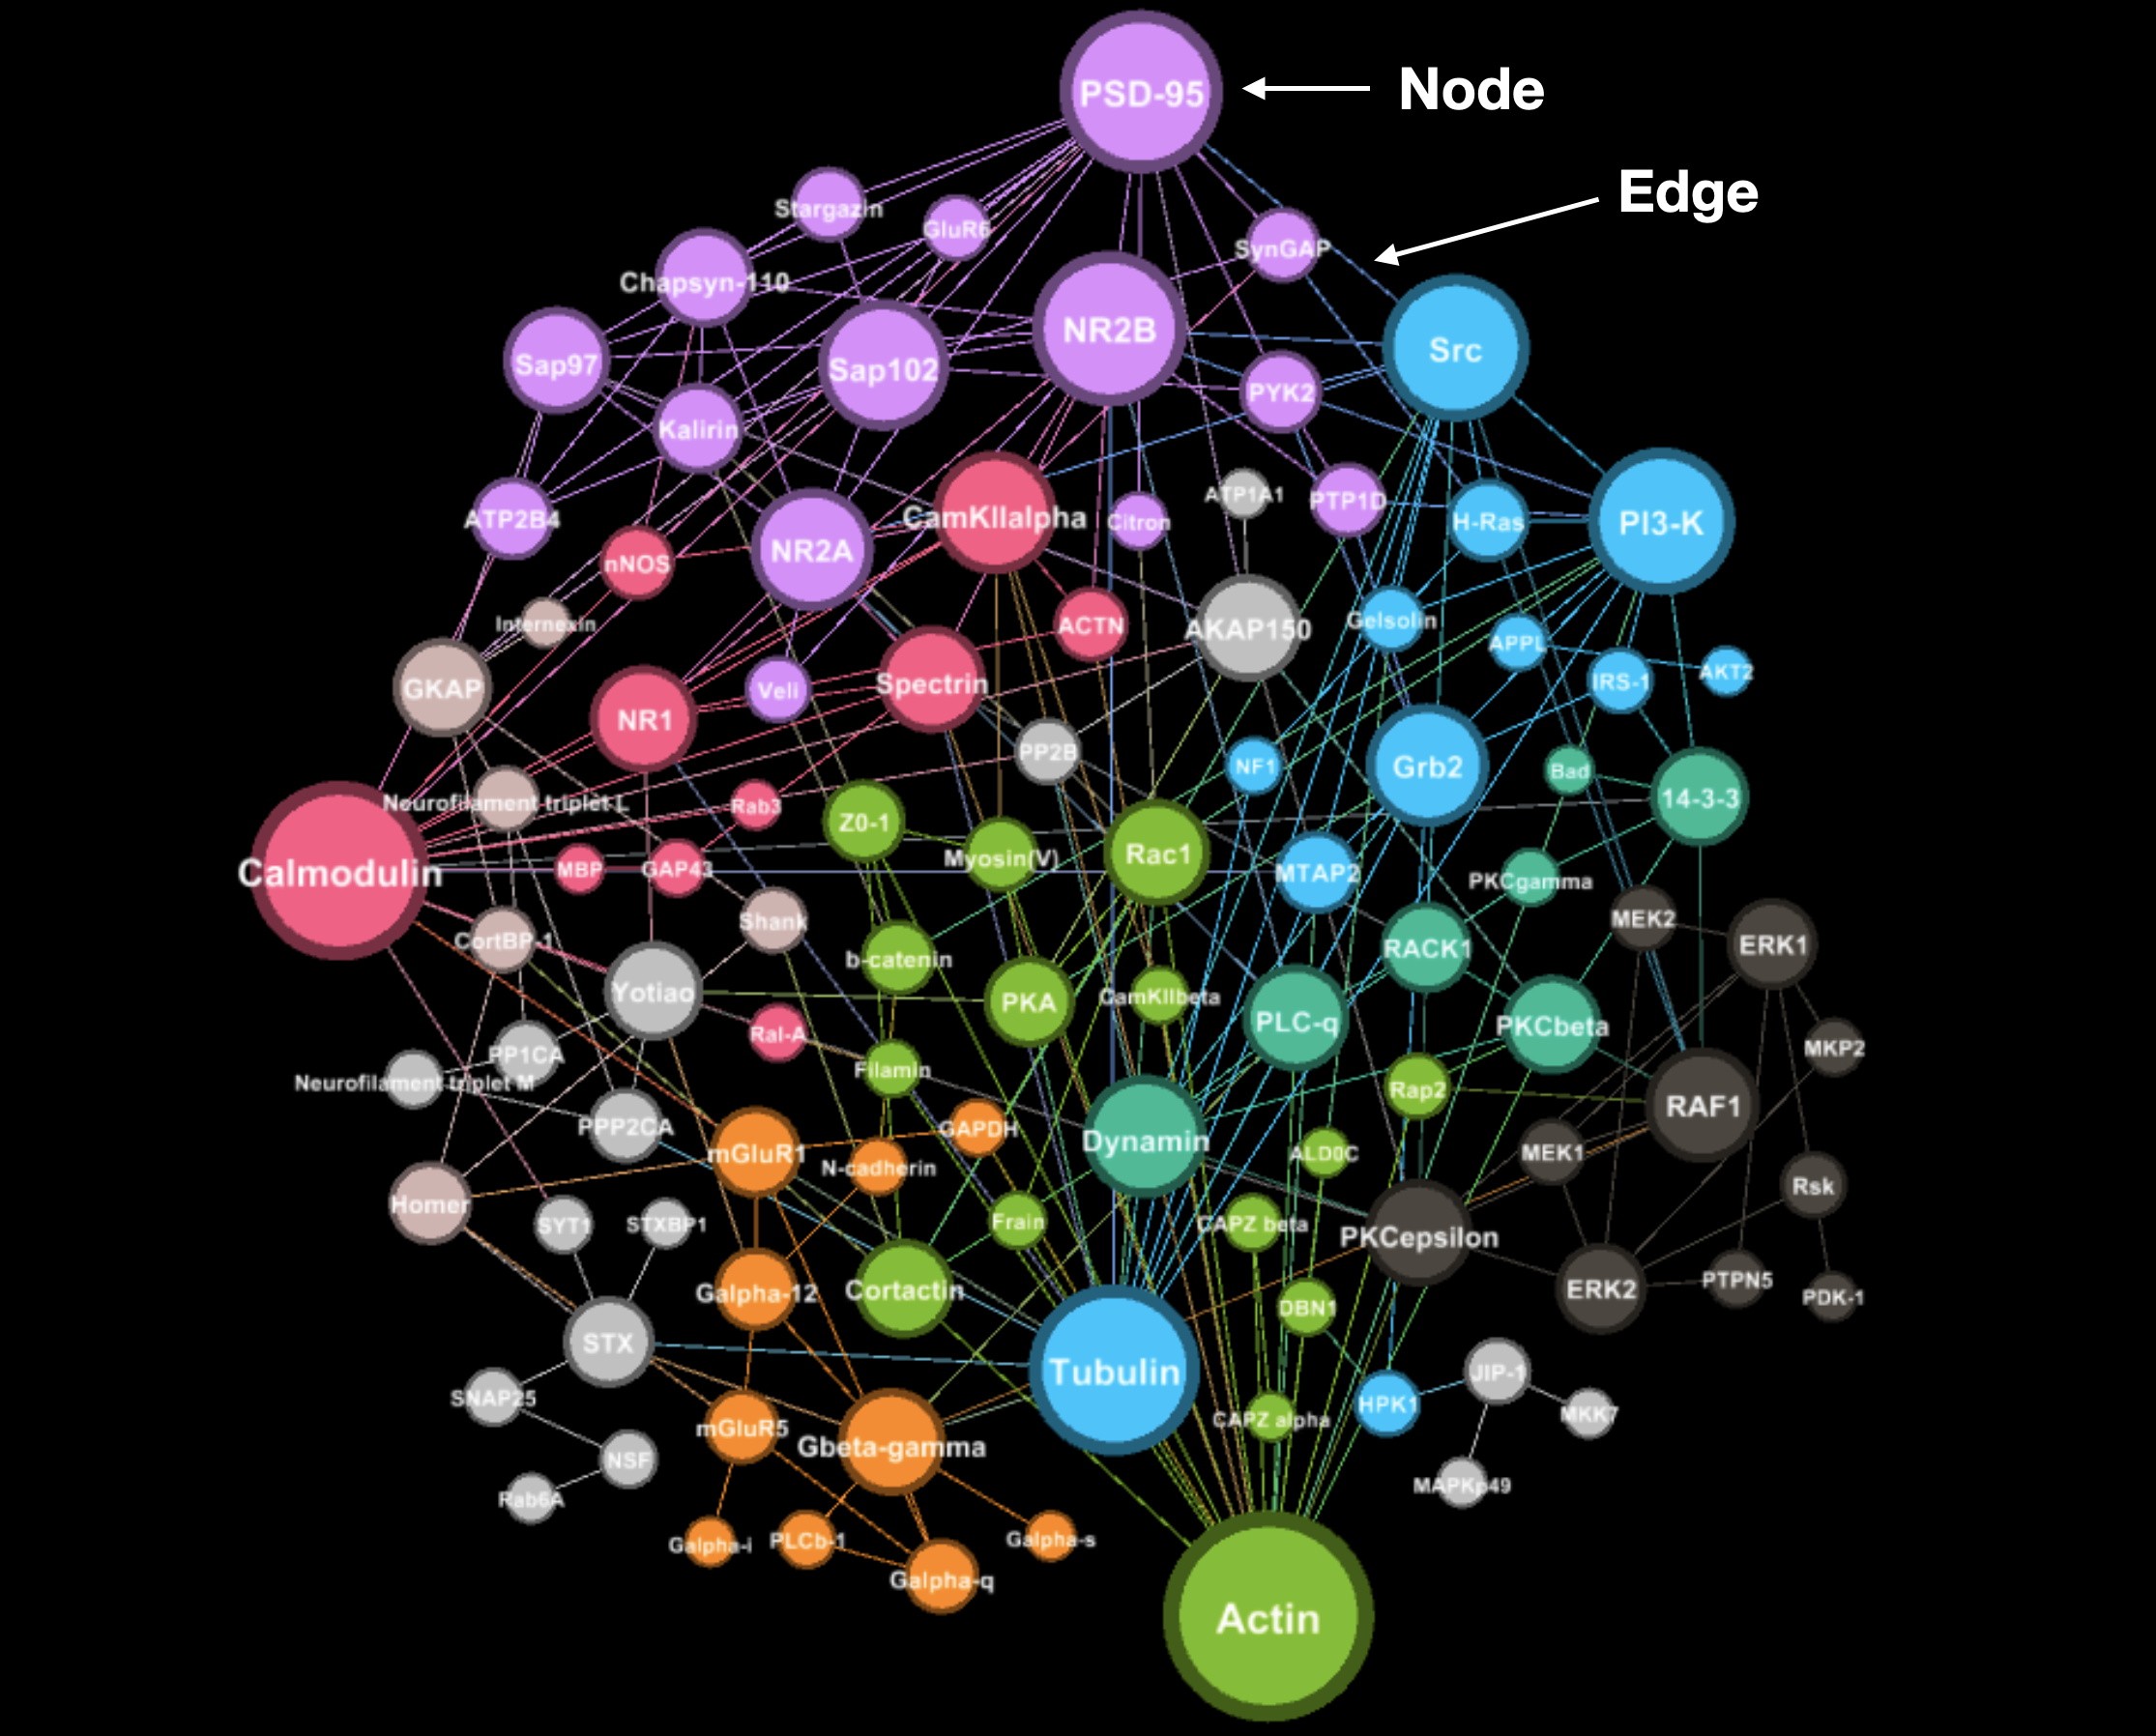
\includegraphics[width=\textwidth]{images/nrc_arrow.png}
        \caption[Network graph of the NRC MASC complex.]{Network graph of the NRC MASC complex. Arrows show a node or vertex which correspond to a gene encoding NRC MASC protein and an edge or link between two nodes which shows that the proteins interact. The network is that described by Pocklington et al. \cite{pocklington2006proteomes} used in the paper by McLean\cite{mclean2016improved}.\footnote{the gml file was produced by CMcL}. Graph visualisation in Gephi\cite{bastian2009gephi} with colours corresponding to community membership. Node size is proportional to degree (the number of edges connected to a node)}
    \label{fig:nrcmasc}
\end{figure}


Protein-protein interaction networks are built using evidence of molecular interaction between the proteins constituting the network. Evidence that proteins interact is
%\footnote{?is - evidence is singular}
curated in protein-protein interaction databases. Human protein-protein interaction databases include those that map to primary proteomic experiments:   the Dictionary of Interacting Proteins (DIP) \cite{salwinski2004database}, MIntAct\cite{orchard2014mintact} and BioGRID \textit{(Bio}logical\textit{G}eneral \textit{R}epository for \textit{I}nteraction \textit{D}atasets)\cite{chatr2017biogrid}; those that contain computational predictions of interactions; and those that contain both, such as STRING\cite{szklarczyk2019string}.

 An alternative division is between primary databases reporting the results of proteomic experiments and meta databases that combine primary databases and may include computational predictions \cite{dong2018analyses}. Experimental evidence for interactions comes from high throughput or low throughput studies. High throughput methods include affinity purification mass spectrometry and two-hybrid screening \cite{dong2018analyses}. High throughput studies constitute the minority of publications curated in databases but account for most of the interactions. For example, in the IntAct database \cite{hermjakob2004intact}, 78\% of publications report 1-10 interactions, but these constitute only 4\% of the interactions in the database \cite{dong2018analyses}. Conversely, only 2\% of studies report over 100 interactions, but these supply 77\% of the interactions in the database \cite{dong2018analyses}.  To permit efficient data sharing a common database schema was developed by the Molecular Interactions workgroup (MI) of the Human Proteome Organisation (HUPO) Proteomics Standard Initiative (HUPO-PSI-MI) in 2002 using a controlled vocabulary to record information on protein interactions indexed with accession numbers \cite{orchard2012molecular}. In addition to a tab, delimited text format (MITAB) there is a stable XML format (PSI-MI XML), allowing a variety of tools to parse information from these databases \cite{orchard2012molecular}.  Protein-protein interaction databases differ due to differences in detection technology and in how experimental data is recorded (curation). The International Molecular Exchange (IMEx) consortium seeks to establish common curation rules and to avoid redundant curation of interactions by coordinating curation across members \cite{orchard2012molecular}, \cite{orchard2012protein}.
 

Despite the use of a standard, machine-readable vocabulary, there is only moderate overlap between the entries in protein interaction databases\cite{dong2018analyses} \footnote{although some of this is due to non-redundant curation} (see table~\ref{tab:overlap between protein interaction databases}). In order to generate a comprehensive network, data must be harmonised from more than one database.  % \textcolor{red}{New} 
In order to provide a comprehensive map of a proteome, several primary databases need to be integrated \cite{alonso2019apid}.%\footnote{note to Douglas/self - this may not be the best reference for this, but it does refer to it}.
Meta databases combine primary databases and may include data from computational predictions, but their evidence base is heterogeneous, and some curation is still necessary to provide an accurate, consistent network.

This is a non-trivial task due to well-documented problems including the use of multiple identifiers, incomplete overlap in experiments, differences between matrix and spokes models and different confidence thresholds \cite{lehne2009protein}.  Network curation is reviewed in depth by Dong and Provart \cite{dong2018analyses}.

  \begin{table}[]
       \centering
       \begin{tabular}{lllll}
       \toprule
    &    BioGRID    & DIP & IntAct & MINT   \\
    \hline
    Interactions & 506,234 & 81,731 & 659,284 & 125,464\\
    \hline
    Species & 62 & 834 & 980 & 611 \\
    \midrule
    BioGRID &  & 13\% & 41\%& 18\%      \\
    DIP & 19\% & & 32\% &20\% \\
    IntAct& 32\% & 10\% & 23\% \\
    MINT 48\% & 26\% & 100 \% & \\
    \bottomrule
       \end{tabular}
       \caption[Overlap between protein-protein interaction databases]{Overlap in records between protein protein interaction databases. The table includes all databases used in the final PSP network with the addition of MINT for purposes of illustration. The table is asymmetric and should be read down the columns as the amount of the \textit{row name} (for example \textit{MINT}) contained in the \textit{column name} (for this example \textit{IntAct}; 100\%). MINT has been included as an example and is a subset of IntACT. All of MINTs interactions are in IntAct so the row MINT, column IntAct; is 100\% but the column IntAct, row MINT is 23\% as the contents of MINT account for this amount of IntAct. Modified from figure 3 in Dong and Provart (2018) \cite{dong2018analyses}.}
       \label{tab:overlap between protein interaction databases}
   \end{table}
 \subsection{Documenting interactions}
 Protein-protein interactions for the PSP network were obtained from the mining and harmonisation of data from the Database of Interacting Proteins (DIP) \cite{xenarios2002dip},  IntAct database \cite{orchard2014mintact},  BioGRID \cite{chatr2017biogrid}, and HIPPIE\cite{schaefer2012hippie}. HPRD\cite{keshava2009human} was excluded as it did not comply to PSI-MI TAB  standards at the time of compilation of the graph. HIPPIE was ultimately excluded from further analysis due to a lack of specific interaction information. See Heil (2018) \cite{heil2018systems} chapter 4 for full details. 
 
 The mapping of identifiers and accession numbers across different databases is a central bioinformatics task \cite{huang2011comprehensive}. These can be different identifiers for a particular object (such as HGNC Gene Symbols or Entrez Gene ID) or mapping identifiers between related objects (e.g. between a protein accession identifier and that of the encoding gene). The mapping of identifiers from UniprotKB to Entrez Gene ID was the most commonly used task in a protein identifier mapping service\cite{huang2011comprehensive}.
 
 A bi-map was created to translate between protein identifications mapped to Uniprot accession numbers\cite{uniprot2017uniprot}, and the GeneID provided by the Entrez Gene portal at the National Centre for Biotechnology Information (NCBI). NCBI Entrez Gene GeneIDs are unique integer identifiers and were used as the main identifier for all subsequent data tables and analyses \cite{maglott2005entrez}. For brevity I use Entrez GeneID synonymously with NCBI Entrez Gene GeneID.
%  \footnote{to remove: comment this might seem pedantic but Enrichr which is very highly cited and otherwise very good enrichment service asks for Entrez ID symbols - looking for Gene Symbol}.
 The widespread use of Entrez Gene identifiers in genomic studies and genomics software \cite{huang2011comprehensive} makes them a suitable primary identifier for network nodes.

Protein-protein interactions were included if there was high quality evidence for direct physical interaction in humans. The interaction list was filtered to ensure all proteins had a human taxonomy ID of 9606. The details of interactions were recorded in PSI-MI TAB 2.5 format (MITAB25)
%\footnote{it is i think PSI-MI TAB 2,5 and MITAB 25 see \url{https://github.com/HUPO-PSI/miTab/blob/master/PSI-MITAB25Format.md}}
\cite{isserlin2011biomolecular}\cite{heil2018systems}. One interaction was retained where mirrored duplicates occurred (e.g. A-B and B-A). The data interaction list resulting contained 396,837 rows and 237,789 unique PPI. 
%\footnote{was a to do I now have got(found) Katharina's document of 2016-10-31 which outlines the interactions strategy for the network. In addition, the document says that spoke expanded PPI from intact were excluded, but perhaps some were found later? so i have not included this yet} 
The interaction list was further filtered to generate the protein interactions represented by edges in the network graph. Protein-protein interactions were excluded if there was no direct experimental evidence of interaction documented by Proteomics Standard Initiative - Molecular Interaction ontology terms in the databases. PSI-MI is a structured ontology used to describe the evidence for protein-protein interactions.\cite{isserlin2011biomolecular} PPIs based on `genetic interactions' (MI:0208) , `genetic interference' (MI0254), `genetic interaction' (MI:0208)\footnote{which includes suppression (MI:0796 and synthetic MI:0794)} and `co-localisation' were excluded (MI:0403). 66 interaction MI accession codes representing direct interaction were included, including one obsolete term `physical interaction' (MI:0218). The final filtered list contained 352,325 unique rows representing 205,461 binary interactions.

  
% Departmental documents on network generation are contained in the following footnotes and will be removed from the final manuscript\todo{FINAL:remove}.
% \footnote{Strontium colin note \url{/home/grant/Documents/PhD_from_DICE/DocSynch_paper_data_dice/data/graph/_from_Colin_Dec_gmlandxls}}
% % \footnote{  Copy of readme
%   Hi Oksana,
% Commented out below
% Attached are initial clustering \& enrichment results (please see below) for the published pre- and post-synaptic lists (Synaptic proteome Dropbox folder) using  Kat's PPI list (file \url{"PPI\_human\_direct\_final.csv}", 31/10/2016).

%  synaptic lists:
%  1) PPI\_Presynaptic\_Published (output .xls \& .gml files)
%  2) PPI\_PSD\_clean\_Published   (output ditto)

%  I guess this is a start. There's details, basic stats i'll need to collect on the clustering results, but hope this helps Kat \& Grant with with there studies, and Oksana to help understanding the clustering in the networks. I'm quite interested looking at the overlap between the different algorithms.
% Let me know if there's any problems? }


\subsubsection{Proteomics data}
\label{sec:proteomics data}
%\todo{there is a repetition somewhere below of the number of studies}
39 proteomic studies conducted between 2000-2017 of the human, mouse and rat synapse were curated into a list of 6500
%\todo{check now} 
potential synaptic genes (all mapped to human Entrez Gene GeneIDs)\cite{heil2018systems}\cite{maglott2005entrez}.  Of these studies, 17 (see table~\ref{tab:Katharina_phd_studies_oksana_studies})
%\{Douglas: See note on text it is either 23 (Kat) table~\ref{tab:Katharina_phd_studiesFF} or 17 (Oksana cleaned file), there is not much difference other than the number of papers covering each protein, the Oksana one is cleaner but there were other nodes in an xls file colin used for the PSP (although they don't appear in the graph he produced}, 
% \{was a todo now a  saying check now it originally was 22 now 23 and four more were added in 2017 to this set which then made up the set that colin gave me based on the Oksana clean published PSD document both included in supplementary material}
% ,
% \{So in Katharina but not in the Oksana listLi 2003Focking 2016Doscemi 2006Distler expectedUezu 2016assuming that Focking is Framer  oksana = 17Katharina = 24 - 1 distler = 23 which is correct from the original paper now missing from the dropbox that I took the original introduction from (of these 23 examined the PSD - it varies i think from 22 to 23 on the doscemi?}

examined the post synaptic density (PSD).
an electron dense structure beneath the post synaptic membrane \cite{PALAY1956}  consisting of complexes of neurotransmitter receptors and their supporting proteins. \cite{kennedy2000signal}  Affinity purification against common PSD proteins improves their identification. \cite{ewing2007large}  
The human proteins and human orthologues of murine proteins found in these studies were used as a ‘parts list’ for the PSD and associated interacting proteins expressed in the post synaptic area (PSP). 3894 genes were identified 
%\{in the 23 studies shown in table~\ref{tab:Katharina_phd_studiesFF}} in the 17 studies (table~\ref{tab:Katharina_phd_studies_oksana_studies}).
%\footnote{ "CHENG   2006"      "DOSEMECI   2006"   "JORDAN  2004"     "LI  2004"        
%  [7] "PENG  2002"       "SATON  2002"      "SCHWENK  2013"    "SELIMI   2009"     "TRINIDAD  2005"   "TRINIDAD  2008"  
% [13] "WALIKONIS  2000"  "YOSHIMURA"       "FROMER 2014"     "FARR.2004"       "Distler.PSDII"   "BAYES 2011"     
% [19] "BAYES 2012"      "COLLINS 2006"    "DOSEMECI  2007"   "FERNANDES  2009"  "BAYES 2014"  }   

 The nodes in the network used in this thesis are genes encoding proteins discovered in the proteomic studies in table~\ref{tab:Katharina_phd_studies_oksana_studies} which have high quality experimental direct interaction data in humans  %\footnote{one study has been removed because it did not meet some of the quality control procedures for the graph generation} 
 (see Heil \cite{heil2018systems} for detailed inclusion criteria and further discussion of network generation.)
% %\footnote{Full text at  ERA link for Katharina PhD \url{https://era.ed.ac.uk/handle/1842/31043} Direct link \url{https://era.ed.ac.uk/bitstream/handle/1842/31043/Heil2018.pdf?sequence=1&isAllowed=y}  p98 fig 5.9a, p86 and supplement C change to era ref},\footnote{previous fulltext link \url{http://www.diva-portal.org/smash/get/diva2:1194151/FULLTEXT01.pdf}} 
The complete network graph contains 3473 vertices and 30499 edges. 
 
% [7] "PENG  2002" \cite{peng2004semiquantitative}  is 2004
% "SATON  2002"   is SATOH 2002 \cite{satoh2002identification}

% "SCHWENK  2013"  \cite{schwenk2012high} 2012
% "SELIMI   2009" \cite{selimi2009proteomic} 
% "TRINIDAD  2005 \cite{trinidad2005phosphorylation}"  
% "TRINIDAD  2008" \cite{trinidad2008quantitative} 
% [13] "WALIKONIS  2000" \cite{walikonis2000identification} 
% "YOSHIMURA" 2004 \cite{yoshimura2004molecular}   
% "FROMER 2014" Not in Heil I only find fromer in an oksana paper on PSD and it is on scz I assume this is Focking and the one cited in Heil is bipolar
% and they have 2033 PSD proteins Focking \cite{focking2016proteomic}
% "FARR.2004" \cite{farr2004proteomic}
% "Distler.PSDII" \cite{distler2014depth}
% "BAYES 2011"   \cite{bayes2011characterization}  
% [19] "BAYES 2012" \cite{bayes2012comparative}    
% "COLLINS 2006" \cite{collins2006molecular}
% "DOSEMECI  2007" \cite{dosemeci2007composition}
% "FERNANDES  2009" \cite{fernandez2009targeted}
% "BAYES 2014"  \cite{bayes2014human}




%  "PENG  2002" \cite{peng2004semiquantitative}  is 2004
% "SATON  2002"   is SATOH 2002 \cite{satoh2002identification}

% "SCHWENK  2013"  \cite{schwenk2012high} 2012
% "SELIMI   2009" \cite{selimi2009proteomic} 
% "TRINIDAD  2005 \cite{trinidad2005phosphorylation}"  
% "TRINIDAD  2008" \cite{trinidad2008quantitative} 
% [13] "WALIKONIS  2000" \cite{walikonis2000identification} 
% "YOSHIMURA" 2004 \cite{yoshimura2004molecular}   
% "FROMER 2014" Not in Heil I only find fromer in an oksana paper on PSD and it is on scz I assume this is Focking and the one cited in Heil is bipolar
% and they have 2033 PSD proteins Focking \cite{focking2016proteomic}
% "FARR.2004" \cite{farr2004proteomic}
% "Distler.PSDII" \cite{distler2014depth}
% "BAYES 2011"   \cite{bayes2011characterization}  
% [19] "BAYES 2012" \cite{bayes2012comparative}    
% "COLLINS 2006" \cite{collins2006molecular}
% "DOSEMECI  2007" \cite{dosemeci2007composition}
% "FERNANDES  2009" \cite{fernandez2009targeted}
% "BAYES 2014"  \cite{bayes2014human}
% in Katharina 
% Doscemi 2006




\begin{table}[]
    \centering
    \begin{tabular}{lllllll}
    \toprule
     & First author & Year & Reference & Region & Species & $n$ \\
    \midrule
1 &    WALIKONIS &2000 &Walikonis et al. (2000)\cite{walikonis2000identification} &postsynapse & rat & 29 \\
2 &PENG&2004&Peng et al. (2004) \cite{peng2004semiquantitative}&postsynapse& rat& 325\\
3 &SATOH&2002&Satoh et al. (2002)\cite{satoh2002identification}&postsynapse &mouse &45\\
4 &YOSHIMURA&2004&Yoshimura et al. (2004)\cite{yoshimura2004molecular} &postsynapse& rat &435\\
5 &FARR&2004&Farr et al. (2004)\cite{farr2004proteomic}&postsynapse &rat &71 \\
% 6 &JORDAN&2004&Jordan et al. (2004)&postsynapse &mouse and rat &390& NOT\\
% 7&LI&2004 &wan Li et al. (2003)&postsynapse &rat& 137& NOT\\
6&TRINIDAD&2005 &Trinidad et al. (2005) \cite{trinidad2005phosphorylation}&postsynapse&mouse& 234\\
% 9&CHENG&2006&Cheng et al. (2006)&postsynapse& rat& 288& NO\\
7&COLLINS&2006&Collins et al. (2006)\cite{collins2006molecular}&postsynapse &mouse& 717\\
% 11&DOSEMESI&2006&Dosemeci et al. (2006)&postsynapse& rat& 113& NO\\
8&DOSEMESI&2007&Dosemeci et al. (2007)\cite{dosemeci2007composition}&postsynapse& rat& 548\\
9&TRINIDAD&2008&Trinidad et al. (2008) \cite{trinidad2008quantitative}&postsynapse& mouse& 2150\\
10&SELIMI&2009&Selimi et al. (2009)\cite{selimi2009proteomic} &postsynapse &mouse &61\\
11&FERNANDEZ&2009&Fernández et al. (2009)&postsynapse& mouse &292\\
12&BAYES&2011&Bayés et al. (2011)\cite{bayes2011characterization}&postsynapse &human &1441\\
13&BAYES&2012&Bayés et al. (2012)\cite{bayes2012comparative}  &postsynapse &mouse &1545\\
14&SCHWENK&2012&Schwenk et al. (2012)\cite{schwenk2012high} &postsynapse &unknown &34\\
% 19&DISTLER PSD1*&2014&Distler et al. (2014)&postsynapse& mouse& 3545& NO \footnote{intended per email}\\
15&DISTLER PSD2*&2014&Distler et al. (2014)\cite{distler2014depth}&postsynapse& mouse& 2092*\\
16&BAYES&2014&Bayés et al. (2014) \cite{bayes2014human}&postsynapse& human &1141\\
% 22&UEZU&2016&Uezu et al. (2016)&postsynapse &mouse &1111 &NO\\
 17&FOCKING&2016&Föcking et al. (2016)\cite{focking2016proteomic}&postsynapse& human &2026\\

\bottomrule
    \end{tabular}
    \caption[Primary Proteomic studies contributing to the PSP - from Heil (2018)]{Primary proteomic studies contributing to the PSP Clean Published network adapted from Heil 2018\cite{heil2018systems} PhD 
    %\footnote{to Douglas: These should have been the same as given to me as per email from Colin need to chose one see note on text. Distler PSD1 is definitely dropped from the cleaned data. The graph is somewhere between these two points. The most conservative is the Oksana one.}
    }
    \label{tab:Katharina_phd_studies_oksana_studies}
\end{table}







 
3475 genes had high quality interaction information available and formed the vertices of the PSP; these included two duplicate Entrez Gene Id and 16 genes that were isolated components and not in the largest connected component).




 
  




 
 
The largest connected component of the resulting graph was used for community detection and in calculating network statistics (3457 nodes, 30498 edges). The details of the small number of excluded vertices not part of the largest connected component are in section~\ref{sec: PSP graph connected component and missing} below.

The methods used to generate the network of the graph are described in detail in Heil (2018)\cite{heil2018systems}. The vertex and edge lists are available in Supplementary material X (along with other data on network generation).

%\footnote{oksana data at\url{/home/grant/Documents/PhD_from_DICE/DocSynch_paper_data_dice/data/graph/_Oksana_synaptic}}
% %\footnote{code to analyse this on Code strontium (informatics workstation) \url{source('~/RProjects/readPSP_data/R/PSPgraph.R')}} \footnote{Counts in literature counter1
% counter
%   1    2    3    4    5    6    7    8    9   10   11   12   13   14   15   16   17   18   19   20 
% 1396  626  339  262  191  156  112   99   76   45   44   35   22   14   16   13    7    4    1    1 }
% %\footnote{counter2 Count of studies not in PSP (so PPI information not available)

%   1   2   3   4   5   6   7   8  10  12  13 
% 250  81  30  31  15  12   7   4   3   1   1 }. 


The network was stored as a named edge list consisting of two columns. Each row represents an interacting protein pair and each protein is identified using the Entrez Gene Id of its encoding gene. Network metadata and interactions were stored as a graph modelling language (GML) file generated from this edge list. \cite{himsolt1997gml}

% \footnote{Original available at \url{https://web.archive.org/web/20190303094704/http://www.fim.uni-passau.de:80/fileadmin/files/lehrstuhl/brandenburg/projekte/gml/gml-technical-report.pdf}}



GML is an ASCII based, hierarchical, lightweight format supported by igraph \cite{csardi2006igraph}, Gephi \cite{bastian2009gephi} , NetworkX \cite{hagberg2008exploring} and graph-tool \cite{peixoto_graph-tool_2014}.  A master copy of the original file supplied to me was stored on the University of Edinburgh informatics server. The original gml file was generated by CMcL and is included in the supplementary material.

%\textcolor{red}{commented out}
% For certain packages the edge list was used or the edge list transformed to an adjacency matrix or other graph object (eg SNAP format)

% Previous note commented out below (list from colin with the 27 had 5101 genes)\footnote{
% for combined list of genes (5101) including both Distler, we have got the PPI information for 3457 genes, which resulted in the graph of 3457 nodes and 30499 edges. Of this - 3457 nodes and 30498 edges contributed to Largest connected component (I guess the same size as initial graph). The majority of genes that survive quality control are expressed in more than one study) Of those in only one study 489/3457 = 14.1\%. 352 appear in the 2014 paper by Distler et al. You have a total of 5101 and of these 1640 appear only once of the 1643 genes that did not makes the final graph 1151 (70\%) were expressed only once 286 twice and 76 three times "

% Those that appeared in the overall graph but not in the LCC appeared on one occasion 2, 2 occasion 2, 3 occasion 6, 7 occasion 1, 8 occasion 2, 9 occasion 3) so there were nodes that we had PPI information for that still did not make it into the LCC so a lot of the ones that did not make it is because we did not have PPI information that met PPI or the genes missed other qc. 

% Yeah cos the ones that appear once we have information on we might even have their degree they are not all going to have degree one so its a subgroup of the proteomics where we have valid PPI - got it. Comparisons between the number of representations in the literature and gene features are described in depth in Heil} \cite{heil2018systems}.\textcolor{red}{endremove}
% \todo{could do correlation in number of representations and pLI and GTex}

\subsubsection{Value of tissue specific networks}
\label{sec:value_of_tissue_specific_networks}

The post synaptic proteome network is tissue specific; it is the network of interacting proteins found in the post synaptic area. I will, as part of overall quality control confirm in section~\ref{sec:gtex profile of PSP genes} that these genes are differentially expressed in the CNS in humans given the marked expansion in the number of genes found in the PSP in this network.

It is desirable to use a tissue specific network as different tissues contain different proteins and therefore different nodes and edges in their proteome network. In some tissues this is can be accepted as a minor simplification of the network model, but other tissues are known to have very different gene expression patterns (e.g solid tissues and blood, CNS \cite{mele2015human}). Statistics describing the proteome network found in different tissues will therefore be different. Secondly, it has been reported that disease genes tend to be expressed in specific tissues (and to be on the periphery of cellular networks)\cite{barabasi2011network},\cite{kitsak2016tissue}. Finally, the synaptic proteome \textit{in particular} has a modular structure arising from the interaction of its protein components and giving rise to higher order structures and functions \cite{pocklington2006organization},\cite{grant2012synaptopathies} that are particular to the synapse. 

I examine this in more detail in the discussion but here give two examples. Ghiassian et al. (2015) \cite{ghiassian2015disease} performed an analysis similar to the one presented here (see section~\ref{sec:intro other approaches}) before going on to describe a method for identifying disease modules.
%A co-author of one of the papers discussing tissue specificity of disease genes\cite{kitsak2016tissue}) 
Using a network made up of heterogenous components to examine several diseases and concluded that topological groups are unhelpful but that diseases result from loss of function of an area of a \textit{global interactome} where a group of disease associated genes reside. 


 Conversely Parishhak (2015) in a review of systems biology \cite{parikshak2015systems} quotes the example of a tissue specific cardiac PPI used to investigate long QT syndrome (LQTS) by Lundby et al. \cite{lundby2014annotation} as an example of the value of tissue specificity. Lundy et al. used a mouse cardiac protein network derived from High Performance Liquid Chromatography Tandem Mass Spectrometry (HPLC-MS/MS) of 5 seed proteins encoded by genes identified in GWAS of LQTS to generate candidate genes later confirmed in zebra fish. These genes could not be identified using more general networks. %\footnote{to discussion - interestingly these are ones in the neighbourhood of receptors and ion channels}.
 See discussion section~\ref{sec:Methods Discussion}.  



\subsection{Connected component}
\label{sec: PSP graph connected component and missing}
Random generative models of networks are often used to study network behaviour \cite{newman2018networks}. The simplest model of a network is the Erd{\H{o}}s - R{\'e}nyi\cite{erdHos1960evolution} model in which each node is connected to every other node with a uniform probability $p$. %\todo{cross ref to Poisson}.
This simple model shows a spontaneous aggregation of isolated nodes to form a large connected component  (connected in that all of its nodes can be reached via `hops' along its edges) containing the majority of nodes  as the average degree (degree $k$, average degree $<k>$) increases.  In real world networks a largest connected component is observed of varying size but there is always one component that dominates the others ($S$, the proportion of nodes in the component) varies - see Newman \cite{newman2018networks}.
\paragraph{Methods}
The network containing all nodes including those not in the largest connected component was generated by CMcL and stored as a gml file. Components were identified using the \texttt{components} command for igraph version 1.2.5\cite{csardi2006igraph} for R and the components not part of the largest component recorded %\footnote{\url{source('~/RProjects/network_graph/R/notLCC_gmt/genes_not_inLCC.R')}}. 

 igraph for R version 1.2.5 was used for the majority of graph processing tasks in scripts using R\cite{csardi2006igraph}. R version 3.6.3\cite{ihaka1996r} is used throughout and  all statistical analysis are carried out in R unless otherwise stated. On some occasions igraph for Python was used typically when methods were only available in Python (such as generating empirical clustering objects to calculate performance measures for community detection (see section~\ref{sec:NMI communities}). This is noted in the appropriate methods sections and in the associated scripts.

Nodes not in the connected component are excluded from further analysis as community detection algorithms and most vertex statistics are not designed for unconnected components.

The composition of the excluded components was analysed to assess whether they contained elements that might bias the subsequent analyses (see section~\ref{sec:analysis of genes not in largest component}).% \todo{do GSA for these componentDONE}
For further discussion of the  connected component see section~\ref{sec:connected component and degree}. 

\paragraph{Results}
In addition to the large connected component ($n$=3457 nodes), 15 smaller components were found within the PSP graph; these were all single isolated components other than one component of size 2.  The  proteins encoded by these genes appear in the ``parts list" derived from proteomic studies but lack experimental evidence of direct interaction with the protein products of the genes in the large component of the PSP.


16 genes were not in the giant connected component and are listed in table~\ref{table:notinLCC}. The only component with two genes contained Oligodendrocyte Myelin Glycoprotein (OMG) and Reticulon 4 Receptor (RTN4R)%
%\footnote{member of growth cone pathway and implicated in scz}. 

 

All but 0.46\% ($S$= 0.995, where $S$ is the size of the giant component expressed as a fraction of total network size - see Newman\cite{newman2018networks} p305 for a comparison with other networks) of the genes identified in proteomic experiments (section~\ref{sec:proteomics data}) with high quality experimental interaction data are part of the largest component. This is comparable to the the undirected metabolic network ( $S=0.996$) in Newman \cite{newman2018networks} \footnote{p 305} but high compared to their example protein interaction network (n=2115,$S$=0.689). Its desirable that a large majority of genes should be in the connected component as most community detection methods and centrality measures are invalid for non connected network components and these genes would need to be excluded and could bias the analysis. 
%\todo{So what}\footnote{Code to generate the table is found at \url{'~/RProjects/analyse_DICE_data/R/LCC.R'}}
\subsubsection{Analysis of genes not in largest connected component}
\label{sec:analysis of genes not in largest component}
%\todo[inline]{what is a component}

Gene ontology enrichment analysis of the 16 genes not in the largest connected component was carried out to ensure they did not belong to a common system or component that would bias the analysis. Gene ontology enrichment analysis is widely used in the rest of this thesis and the methods introduced below.


\subsection{Gene ontology analysis}
\label{sec: gene ontology analysis}
A gene ontology provides a controlled, maintained vocabulary to describe sets of genes according to their Biological Function, Cellular Component and Molecular Function. It is widely used in high throughput genetics to provide information on the function of a set of genes \cite{ashburner2000gene}.Gene ontology terms have structured interactions forming a directed acyclic graph that shows the hierarchical relationship between terms with more specific child terms arising from parent terms (see figure~\ref{fig:the DAG of Collateral sprouting}).

Gene ontology over-representation analysis tests whether a set of genes are more commonly annotated to a specific term  than would be expected by chance. Some also  difference in results is reported across different platforms and therefore more than one method is used \cite{rhee2008use}\cite{khatri2005ontological}. 


\paragraph{Multiple testing}
Gene ontology terms overlap, especially at different levels in the hierarchy, are not independent and therefore assumptions of independence in multiple testing corrections are invalid. The issue of multiple testing in Gene Ontology enrichment analysis is complex and beyond the scope of this thesis. Rhee et al. (2008) \cite{rhee2008use} provide a comprehensive summary an a more recent, technical analysis is found in Meijer et al (2016)\footnote{this actually isn't the most technical there is a general treatment for inference in DAG by the same author} \cite{meijer2016multiple}. A brief description is however necessary both to introduce the methods in this chapter and to indicate potential limitations to pathway enrichment methods in general (including MAGMA GSA which make extensive use of ontology terms). 

Rhee et al. (2008) \cite{rhee2008use} recommend the following approach to multiple testing:

`An unbiased search for significant GO associations can be done with a bottom up approach as follows: for every leaf term, calculate p-values with the genes directly associated to it. If any term is significant do not propagate its genes above. This would provide the most specific node that is significant in that particular branch. If a term is not significant, propagate the annotations to its parent and recalculate with the parent term. The genes will propagate upwards until a significant node is found or until the root is reached. A careful analysis is still necessary to properly correct for multiple comparisons.'\cite{rhee2008use}

 To my knowledge there is no widely available implementation of this method designed for genomic analysis the closest being the methods described by Alexa et al.\cite{alexa2006improved} and implemented in topGO\cite{alexa2009gene} (see below).  Rhee et al.\cite{rhee2008use} state that the Bonferroni correction is too conservative and Holm and FDR offer better alternatives. Another method for correction is that implemented in g:Profiler \cite{raudvere2019g} which uses the sgs method for multiple comparisons to increase power given the interdependence of GO terms. 
 Rhee et al. recommend minimising the number of tests wherever possible \cite{rhee2008use}.\footnote{see also }
One way to reduce the number of tests is to use a restricted or clipped Ontology. This can be challenging to implement and although a neural immunology clipped ontology has been described \cite{geifman2010neural} I am not aware of any application providing a clipped neural ontology enrichment however the SynGO project\cite{koopmans2019syngo} uses and ontology restricted to the synapse where gene term relationships are supported by  high quality experimental evidence.

% In practical terms one should be aware that multiple testing using Bonferroni correction (as implemented in MAGMA) is too strict, second that the results of enrichment in hypothesis generating applications do not truly represent an absolute value of the likelihood of a test under repetition but a measure of confidence in specific findings. I will return to this in the discussion.


\subparagraph{elim method}
The \textit{elim} and \textit{weight} methods described by Alexa et al. (2006)   \cite{alexa2006improved} and implemented in the popular topGO R  package\cite{alexa2009gene} have the effect of decreasing the significance of very general GO terms (increase p) in comparison to more specific child terms. These methods proceed upwards from child nodes and only move genes for testing to the next level if they have not been scored at the lower level. This has the effect of decreasing the significance of very general terms and making very specific terms more significant within the  analysis. The general effect is to increase the overall raw p values but to do this most for general terms.  It does not correspond exactly to multiple testing correction but does prioritise general terms and deflate significance of general terms.  The authors state that most multiple comparison methods are too strict given the connected structure of GO and they prefer to regard the \textit{elim} results as already corrected \cite{alexa2020gene}.\footnote{if you look at the results you can see that adding a multiple testing penalty on top of this would be too severe} \footnote{\url{https://bioconductor.org/packages/release/bioc/vignettes/topGO/inst/doc/topGO.pdf} 2020}.
\paragraph{background set}
The number of terms that are expected to be found in a group of genes depends on the background set and this plays an essential role in calculating over representation. Some packages allow the use of custom background sets (ToppGene has very recently \footnote{last 2 weeks} added this feature). If not indicated the background set is the default for that enrichment package usually the protein encoding genes in the genome.  

\paragraph{Common methods}
Some methods use direct data entry to a web interface, others an API and some methods can be locally installed. The main advantage of web based ORA is regular updating of the ontologies and a common computational platform. To reduce transcription errors, whenever text entry of a list of genes is used on a web interface a script is used to write the list of genes directly to the clipboard \footnote{A function calling the Linux command \texttt{xclip} was used in R to transfer the print formatted object to the clipboard\url{source('~/RProjects/paper_xls_output/R/functions_for_project.R')}, while in Python the \texttt{to\_clipboard} function in the data frame analysis pandas module was used\cite{mckinney2011pandas}.} 
\subsubsection{PANTHER methods}
\label{sec:panther methods1}
Gene ontology ORA for the genes not part of the connected component was carried out using the PANTHER classification system (protein annotation through evolutionary relationship) version 15.0\cite{mi2019protocol} via the web-based user interface hosted at the Gene Ontology Consortium (GOC) website\footnote{\url{http://geneontology.org/}}.

%\todo{compress this and put into methods and results}\textcolor{red}{start compress}
PANTHER provides information on gene function at a genomic scale and as a member of the Gene Ontology Consortium provides accurate annotation with regular updates\todo{compare with DAVID}. Results can be displayed showing their relation in the gene ontology hierarchy\cite{mi2019protocol}.  The authors recommend the use of the False Discovery Rate to correct for multiple comparisons because of the correlation between tests involving related annotations \cite{mi2019protocol}. It can be accessed using an API or web application. It was used for tests where authoritative, accurate testing using an up to date ontology were required rather than as part of an automated workflow. PANTHER accepts custom background sets for enrichment.(for example to see whether a set of genes is enriched compared to the whole genome or the rest of the PSP). 

PANTHER 15.0 (released 2020/02/14)\cite{mi2013large} was used to carry out test sets of genes for over representation of terms from each of the three Gene Ontology clades (Cellular Component, Biological Process and Molecular Function).  Versions are identified by release dates using the year, month, date format supplied in the list of reporting details supplied by PANTHER.The PANTHER Over-representation Test used implementing Fishers Exact test (released 2020/07/28).  The Gene ontology database was DOI: 10.5281/zenodo.3873405 Released 2020-06-01.  The Benjamini-Hochberg procedure \cite{benjamini1995controlling} was used to calculate the False Discovery Rate (FDR) to account for multiple comparisons and corrections  were applied for each clade.

\paragraph{Annotations}

Despite using Entrez Gene ID integer values with the recommended string prefix "GeneID:" (as PANTHER interprets integers as HGNC identifiers by default) several genes were not identified using Ensembl and Entrez Gene ID. Entrez ID were therefore mapped to HGNC Gene Symbols. Where Gene symbols were not identified the list of synonyms in Entrez Gene were used until a match was obtained\footnote{also checking that the supplied match maps to correct Uniprot but i say this later and there are scripts for PANTHER searches and a csv containing the accepted symbols mapped to Entrez ID}. 




% PANTHER introduced in section~\ref{sec:panther methods1} is a member of the gene ontology consortium and frequently updated. The results obtained contain links to easily view the GO tree and also present results in terms of the hierarchy. Mi et al\cite{mi2019protocol} in the most recent update acknowledge that given the relatedness of GO terms tests are non independent and therefore the Bonferroni correction is too conservative. As an alternative they recommend using the FDR method.
They also implement SLIM ontologies 





\subsection{Methods}
\label{sec:GO enrichment methods}
% In addition to Panther described earlier I used the ToppFun functional enrichment service which is part of the toppgene suite. The web interface was used but data entry was carried out using a pipeline from GWGAS significance tests to the system clipboard to avoid transcription errors.
% Method - for each generated list of significant genes mapped to 
% Entrez, Symbol, Ensembl, Protein
% \subsubsection{from earlier}

% \todo{Other comments rhee} Rhee\cite{rhee2008use} see notes.rtf on Windows10 path commented out below 
% %%C:\Users\gxrob\OneDrive\Documents
% \textcolor{red}{The issue of multiple testing complicated for gene ontology terms as they form a directed acyclic graph where a child node is derived from a parent term (for example GO:008066 Molecular function glutamate synthesis is a child term of GO:0004888 transmembrane signalling receptor ). The recommended practice in calculating significance is to propogate up the tree until a node achieves significance and not to propagate to ever more general terms\cite{rhee2008use}. It is not clear to me that this is implemented in the enrichment packages using Gene ontology terms reported in the literature for the GWA studies for intelligence and educational attainment used here (eg MAGMA, FUMA). Variations in GO enrichment scores between packages are well recognised and as I have used both PANTHER and topGO below which respect DAG topology it does not change the analysis (however see discussion section)}


For computational calculations of gene ontology where rapid output is required as part of a pipeline I have used topGO version 2.38.1 an R package that provides gene ontology enrichment \cite{alexa2006improved},\cite{alexa2009gene}\footnote{code \url{source('~/RProjects/graph2community/R/topgo/modified_exampleGoObject_groups.R')}}.
specific to it will be described when first used as will be the case with other methods. 
 topGO has the advantage of being a longstanding R package and part of the Bioconductor\cite{gentleman2004bioconductor} universe. It is well suited as part of a computational workflow but suffers from slower updates than PANTHER (and ToppGene) and misses the annotation of certain genes. 


For limited numbers of tests where quality of results is the most important thing I have used the PANTHER database as it is regularly updated, uses high standard corrections that respect the GO tree and is part of the gene ontology project. Results are also available as a hierarchy in gene ontology. 

\subsubsection{PANTHER}
\label{sec:methods GO Pather}
Using PANTHER there were identifiers that were not recognised using Ensembl ID, Entrez ID and GeneID. The most robust appeared to be gene symbol. I used translation from Entrez ID to Gene Symbol including synonyms until all genes were identified. In addition to the code documenting the data transformation \footnote{code \url{ source('~/RProjects/paper_xls_output/R/chapter_2/FUMA/edit_gene_table/EA2_FUMA2clipboard.R')}}, the gene mapping compatible with PANTHER is included in the supplementary materials.    \footnote{with ENSEMBL ID ENSG00000256762 was unmapped as was Uniprotand Q8IWL8 (STH)Entrez translation using FUMA resulted in 2 unrecognised gene symbols MGEA5 and C10orf76. Correcting these manually using lookup for synonyms the table was ommended to OGA and ARMH3 resulting in all 99 genes being correctly mapped. A full gene mapping compatible with PANTHER is available in the supplemental material}

 The PANTHER displays hierarchy of the ontology terms although the FDR values are lower than ToppGene the very specific term related to neurogenesis positive regulation of collateral sprouting (FDR p 0.041) is prominent in comparison to the same data ordered by FDR shown in table~\ref{tab:GO biological process complete Education Replication FDR}. \todo{Panther has a somewhat complicated implementation of the Bonferroni correction that partly takes into account the issues with multiple comparisons but I have not mentioned it as not using Bonferroni and I think it may be new (Wasn't in 2019 update paper)}

 

\subsubsection{ToppGene}
\label{sec:ToppGene GO enrichment}
 Toppgene is a gene enrichment service which also includes murine and human phenotypes and disease enrichment\cite{chen2009toppgene}. It has a regularly updated database. There are differences in absolute enrichment significance values between different methods as found reported by Rhee \cite{rhee2008use} but fewer differences in annotation. Data entry to toppgene was done using Entrez ID as default. The ToppGene translation API implements  HTTP POST and HTTP PUT methods and was used for translation of identifiers and where this has been done it is noted in the manuscript. To reduce transcription errors where the text entry web interface was used this was done using direct writing to the clipboard as described in section~\ref{sec:panther methods1}. The output tables for significant ToppGene analyses including terms searched are included as tab separated text files  in the supplementary materials. ToppGene now allow the choice of a background set. Database update 28-07-20. Gene Ontology Biological Process 16465 annotations 20148 genes. Cellular component  2043 annotations 20584 genes molecular function 4745 Genes 20584 (for full details see supplemental methods). GO ontology from PANTHER DB.  
 
PANTHER allows the use of a custom background gene set to test enrichment against. The main drawback of PANTHER is that it can occasionally fail to recognise common gene identifiers even when presented in their recognised form. For that reason and given the fact that there are well described differences between the results for different enrichment methods I have also used ToppFun in the ToppGene package which provides convenient links to the complete gene list of terms which is useful in chapter 4. It also has a very clean interface and excellent identifier recognition (see discussion for further comments on ease of use). The main drawback of ToppFun is that it does not provide for an easy implementation of a custom background gene set. For importance of frequent updates see \cite{tomczak2018interpretation}.

\subsubsection{topGO}
\label{sec:toponto GO enrichment preliminary}
 topGO has the advantage of being a longstanding R package and part of the Bioconductor\cite{gentleman2004bioconductor} universe. It is well suited as part of a computational workflow but suffers from slower updates than PANTHER (and ToppGene) and misses the annotation of certain genes. 


topGO is an R package widely used to perform Gene Ontology enrichment and is thus very suitable for integration into a computational workflow abd implements the elim method. It is updated less frequently than PANTHER. As it is not used in this chapter a detailed discussion of the methods are contained in section~\ref{sec:Gene ontology topgo}). 
 \subsubsection{SynGO} SynGO (Synaptic Gene ontology and annotations) is available as a web interface for Gene Ontology enrichment\footnote{\url{https://www.syngoportal.org/}}xls files in supplementary material\cite{koopmans2019syngo}. It provides an expert curated evidence based ontology mapping of synaptic genes to Gene Ontology terms and provides a subset of the complete GO ontology. It is provided as a web interface with text or file based entry. It provides a default background list of gene expressed genes. It covers the cellular component and biological function GO clades. Fishers exact test is used for testing over representation with the FDR method\cite{benjamini1995controlling} used to correct for multiple comparisons. The detailed supplemental data outputs in xls format are included in the supplemental materials. 
\subsubsection{FUMA Gene2Func package} 
\label{sec:FUMA go enrichment}

FUMA (Functional Mapping and Annotation of Genome-Wide Association Studies)\footnote{\url{fuma.ctglab.nl}} is a comprehensive web based annotation and analysis packaged.\cite{watanabe2017functional} It has been widely used in the secondary analysis of GWA studies\cite{hill2019combined}\cite{savage2018genome} and implements Gene level GWGAS using MAGMA and provides extensive annotation services. The system divides into a SNP2Gene module takes summary SNP data as an input and Gene2Func module which takes a list of significant genes. FUMA v1.3.6 was used. 

I have used the GTEx expression enrichment analysis from the Gene2Func module. This differs from the results and methods presented in section~\ref{sec:GTEx methods} in using a predetermined set of differentially expressed genes and testing over representation using the hypergeometric test and Bonferroni correction for multiple comparison \footnote{for technical details see\url{https://fuma.ctglab.nl/tutorialgene2func} note the address is tutorial HASH gene2func}. This to provides a quick, graphical representation of the differences in tissue expression of genes in the PSP and genome wide significant genes at GWGAS in the discovery and replication samples.\todo{? add the fuma methods} I have also used the Gene Set Analysis in the Gene2Func module which uses hypergeometric tests to assess over representation of terms. Data sets are provided (including gene ontology terms, Wiki Pathways and GWAS catalogue) with Bonferroni correction per category. I have used the GWAS catalogue set enrichment to ensure that genes excluded from analysis are not potential sources of bias (ie reported in intelligence GWA or other neurocognitive phenotypes).

\subsubsection{g:Profiler} 
\label{sec:gProfiler GO enrichment}
g:Profiler, is a longstanding Gene Ontology Consortium (GOC) backed Gene Ontology functional enrichment package. It has a recently updated web interface and an R API. Over representation of ontology terms is tested using the cumulative hypergeometric test \cite{raudvere2019g} and the g:SCS (set counts and sizes) method which takes into account the overlapping between sets based on GO terms \cite{reimand2007g} used to correct for multiple comparisons. It provides a  Manhattan like plot of over representation and a comprehensive translation service that can be accessed from the R API. Although it includes other data from KEGG and wiki pathways I have limited the analysis to GO enrichment terms (these are tested using ToppGene). 

Functional enrichment was carried out using g:Profiler version e100\_eg47\_p14\_7733820 (database updated on 07/07/2020). Multiple testing was controlled using g:SCS method applying a significance threshold of 0.05\footnote{recommended citation format from website} and not displaying  under-representation.



\paragraph{Results ORA of genes not in connected component}


%\todo[inline]{this must be in strontium}
%%% GENES EXCLUDED AS NOT IN LCC %%%

% latex table generated in R 3.6.2 by xtable 1.8-4 package
% Tue Dec 31 09:25:51 2019/home/grant/RProjects/network_graph
\begin{table}[ht]
\centering
\begin{tabular}{cllc}
\toprule
 
GeneID & Gene Symbol & Gene Name & $n$ \\ 
\midrule
 4974 & OMG & oligodendrocyte myelin glycoprotein & 2 \\ 
  65078 & RTN4R & reticulon 4 receptor & 2 \\ 
 98 & ACYP2 & acylphosphatase 2 & 1 \\ 
  166785 & MMAA & metabolism of cobalamin associated A & 1 \\ 
  549 & AUH & AU RNA binding methylglutaconyl-CoA hydratase & 1 \\ 
  55847 & CISD1 & CDGSH iron sulfur domain 1 & 1 \\ 
  23305 & ACSL6 & acyl-CoA synthetase long chain family member 6 & 1 \\ 
  26027 & ACOT11 & acyl-CoA thioesterase 11 & 1 \\ 
  7915 & ALDH5A1 & aldehyde dehydrogenase 5 family member A1 & 1 \\ 
  4685 & NCAM2 & neural cell adhesion molecule 2 & 1 \\ 
 
  5649 & RELN & reelin & 1 \\ 
  2741 & GLRA1 & glycine receptor alpha 1 & 1 \\ 
  152404 & IGSF11 & immunoglobulin superfamily member 11 & 1 \\ 
 
  27000 & DNAJC2 & DnaJ heat shock protein family (Hsp40) member C2 & 1 \\ 
  2686 & GGT7 & gamma-glutamyltransferase 7 & 1 \\ 
  55262 & MAP11 & microtubule associated protein 11 & 1 \\ 
   \bottomrule
\end{tabular}
\caption[Genes not in largest connected component]{Genes with cognate proteins in the PSP as defined by their presence in proteomic studies but that are not part of the giant connected component. These encode proteins that lack direct experimental evidence of interaction with the giant connected component. GeneID is Entrez Gene ID. $n$ is the number of genes in the component.} 
\label{table:notinLCC}
\end{table}

There is no evidence of any enrichment of an association between genetic variants in the set of 16 genes not in the largest connected component and differences in intelligence or educational attainment in any of the discovery or replication samples (see section~\ref{sec:samples from paper section}) using  MAGMA Gene Set Analysis (see table~\ref{tab:notLCC}; details on methods for MAGMA GSA in section~\ref{sec:Gene set analysis community detection}).

\begin{table}[]
    \centering
    \begin{tabular}{lll}
    \toprule
     Sample   & $\beta$ & p  \\
     \midrule
     Intelligence\textsubscript{Replication} & 0.30 & 0.10\\
     Education\textsubscript{Replication} & 0.11 & 0.32\\
    % ea3     & 0.307 & 0.19\\
    Intelligence\textsubscript{Discovery} & -0.09 & 0.64\\
    Education\textsubscript{Discovery} & 0.21 & 0.21 \\
    \bottomrule
    \end{tabular}
    \caption[MAGMA GSA for network vertices not in largest connected component]{MAGMA GSA enrichment of the set of genes not in LCC n = 16. Testing the competitive hypothesis that genetic variants mapped to these genes are more associated the Intelligence or Educational Attainment phenotypes than the rest of the genome. Code at \url{/home/grant/RProjects/network_graph/notLCC.txt}}
    \label{tab:notLCC}
\end{table}
%%%


\subsection{GTEx profile of PSP genes}
\label{sec:gtex profile of PSP genes}
\subsubsection{Introduction to GTEx}
The gene tissue expression project (GTEx) is a repository of gene expression in over 1000 individuals from 54 tissue areas\cite{lek2016analysis}. I have used this to determine if the PSP genes are predominantly expressed in the brain, if there are significant regional differences in expression that might affect the analysis and that the expression of PSP genes is as expected significantly greater than of those not in the PSP, which will of c
ourse include a number of genes significantly involved in processes in the brain. 

\subsubsection{GTEx Methods}
\label{sec:GTEx methods}
 Gene expression data (GTEx version 8 - dbGaP Accession phs000424.v8.p2) were obtained from: the GTEx Portal on 07/03/2020. Median gene expression counts normalised by Transcripts Per Million (TPM) were downloaded from the GTEx Portal website \cite{gtex2015genotype}.
 \footnote{\url{https://storage.googleapis.com/gtex_analysis_v8/rna_seq_data/GTEx_Analysis_2017-06-05_v8_RNASeQCv1.1.9_gene_median_tpm.gct.gz}}\cite{gtex2015genotype},\cite{conesa2016survey}. The median gene expression values were calculated by the GTEx authors from the file \url{GTEx_Analysis_2017-06-05_v8_RNASeQCv1.1.9_gene_tpm.gct.gz}. 
 
 Two indentifiers were provided for each gene, Ensembl Gene ID (ENSG) and HUGO gene nomenclature committee (HGNC) Gene Symbol\cite{gray2012genenames}. The ToppGene annotation service \cite{chen2009toppgene} was used to provide Entrez gene GeneIDs from Gene Symbol to allow the results to be combined with the synaptic network and cohort study results \todo{may not have mentioned the cohorts yet}\footnote{\url{https://toppgene.cchmc.org/API/lookup}}\footnote{\url{source('~/RProjects/gtex/R/exploratory_gtex/load_toppgene_annotations.R')}}.

56200 rows were downloaded from the GTEx Portal indexed by Ensembl id which included a version suffix and Gene Name (marked as `Description' in the file). Each Ensembl ID including version number was unique 56156 unique ID were found discounting Ensembl version.

199 duplicated gene names were identified in 1608 duplicated GTEx entries. 114 had a single duplicate (a total of two Ensembl id to one gene name). 737 duplicates were identified to Y RNA (45.8\%). Y RNAs are small non coding RNA \cite{perreault2007ro}. 166 were metazoa signal recognition particles (SRP)\cite{keenan2001signal} (10.3\%). 

54592 unique Gene Symbols were found associated with  be unique Ensembl id (97.1\%) of the Ensembl ids.\url{source('~/RProjects/gtex/R/exploratory_gtex/first_load_gtex.R')}\todo{check this in the code DONE} 

To exclude non coding elements  reduce the data size and exclude non coding elements, I used the 18390 genes\todo{and PSP} that have gene level results in at least one of the samples where gene level statistics are calculated in MAGMA. 17584 unique Entrez ID were identified from the remaining elements and used for subsequent analysis.\footnote{Sniekers et al found 44 of the 52 significant genes (using SNP proximity) and MAGMA in GTEx}

Entries were retained if the TPM count was greater than 0.1 in approximately 80\% (79.6\%) of samples. TPM counts were then $log_2$ transformed with a pseudocount of 1 and zero centred  \cite{sniekers2017genome},\cite{taskesen20162d}\cite{mele2015human}\footnote{\url{source('~/RProjects/gtex/R/exploratory_gtex/df_with_toppgene_log_normalise_plots.R')}} \footnote{log transformation and removal levels are standard for RPKM, RPKM are similar to TPM and proportionate, since I wished to compare expression between genes across a common set of samples I kept the method the same however} see \cite{zhao2017gene}. \footnote{Remove: explanation for self \url{https://rna-seqblog.com/rpkm-fpkm-and-tpm-clearly-explained/} Read per kb then normalise (gene length) then normalise by read length (opposite way round to TPM)). Sum of normalised reads same across samples. } \footnote{Current \url{source('~/RProjects/gtex/R/graph_gtex/graph_new_cutoff.R')} includes number of tissues at each cutoff and does multiplot}

\textsubscript{Remove: ok note to self. It is not really possible to measure if gene expression higher in brain for a gene using gtex expression data however this is building on the stuff reported in the intelligence literature which basically uses fuma and they use previous qc for RPKM which is removing expression <0.1 in 20\% of tissues see \url{https://www.researchgate.net/post/What_is_a_valid_way_to_measure_variability_of_gene_expression_from_gtex_data} but all we want to do is to use this as a bit of qc if they are brain expressed genes it is likely they are more differentially expressed in the brain so remove the two main sources of error low expressed genes and heteroscedacity which you would do with mean centring and log transform after any reasonable low filter which removes most low expressed genes. There is a lot of talk about winsorizing (peak clipping) in the literature but the results are from FUMA which gets around this by using a predetermined set of DEG and then testing for over representation among them. Peak clipping will remove outliers and reduced delta variance with delta expression but a lot of gene expression is led by a few highly expressed genes. It seems quite complicated, I don't know very much about it at all, I think the people who know about rna seq probably are the most likely to know what they are talking about, but just about every gwa on int has used this so .. given the limitations above I don't think it is unreasonable to check you don't have an effect going the opposite way to what you think what I am not saying is that this set is y units whi
ch are evenly spaced different from the other}


\begin{figure}
    \centering
    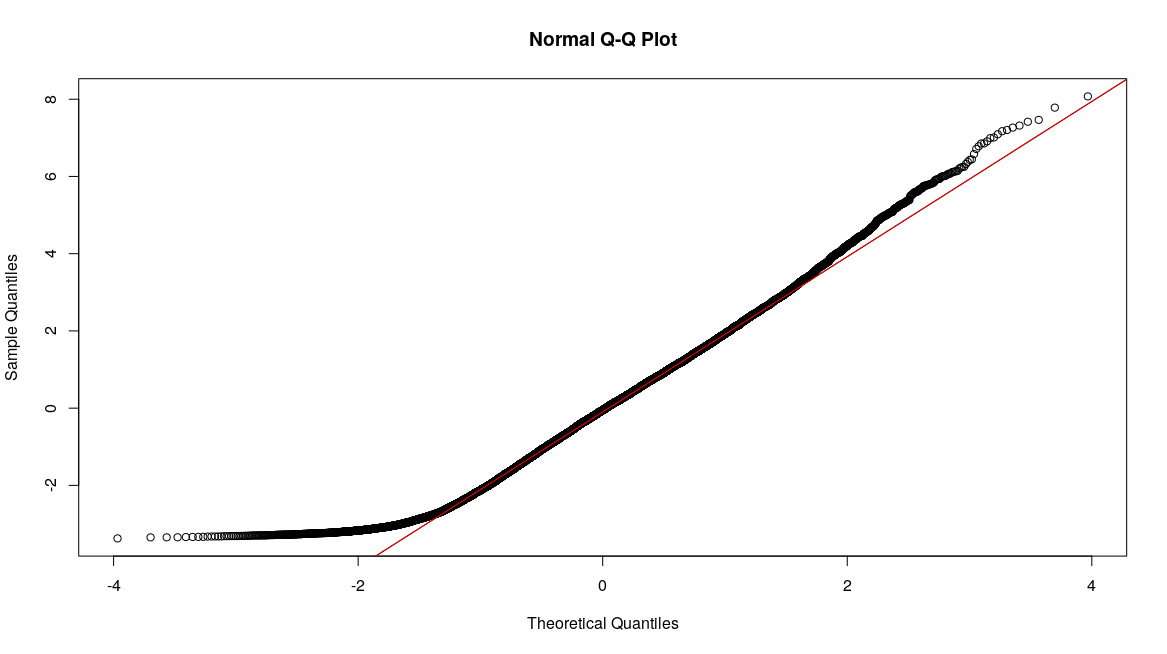
\includegraphics[width=\textwidth]{images/Rplot_rough_qq.png}
    \caption{QQ plot log2 transformed and mean centred gene expression fronal cortex all genes passing quality control 13787 genes}
    \label{fig:qqplot frontal cortex}
\end{figure}

The QQ plot of frontal cortex expression looks relatively normal (see figure~\ref{fig:qqplot frontal cortex}).

\begin{figure}
    \centering
    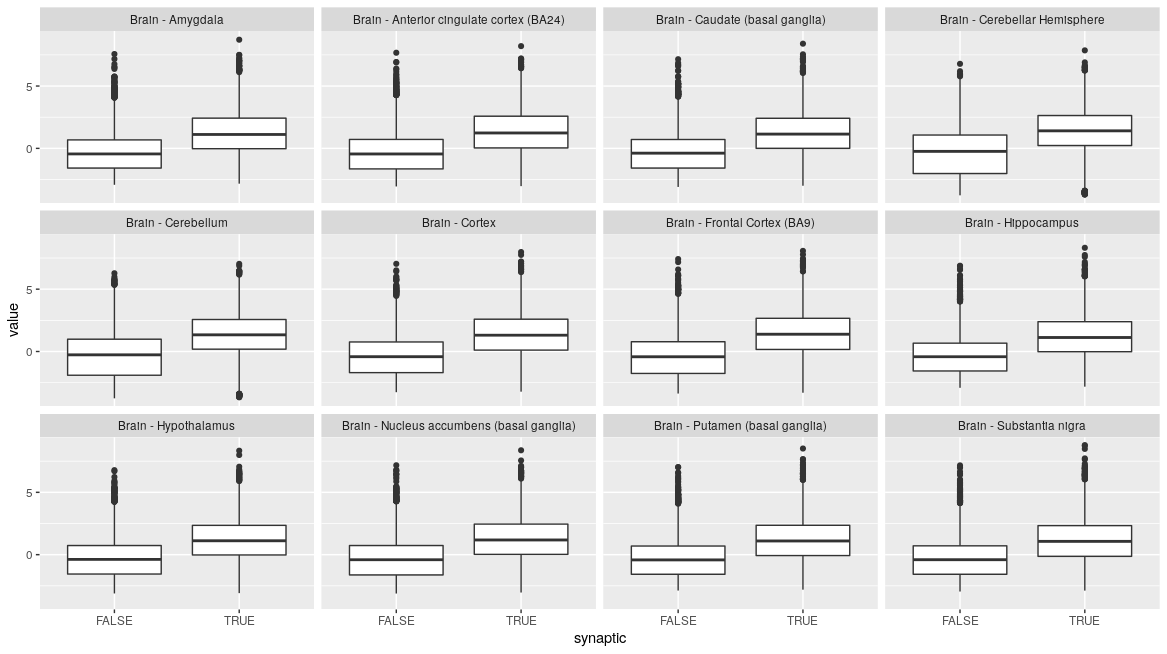
\includegraphics[width=\textwidth]{images/Rplot_compare_expression2.png}
    \caption{Box plot of log2 transformed and mean centred gene expression of PSP genes versus non PSP genes across 12 brain regions. p $< 2 \times 10^{-16}$ all comparisons. Wilcoxon test. True and False on x axis refer to whether genes are PSP in origin. Code at \url{source('~/RProjects/gtex/R/graph_gtex/multi_boxplot.R')}}
    \label{fig:my_label}
\end{figure}

\subsubsection{Results Brain Expression of PSP genes}
\label{sec:gtex_results}
3055 genes with GTEx data passing the above quality control were available for the PSP and 10732 non synaptic genes. 
Expression is significantly higher in the PSP genes across all 12 brain regions (spinal cervical1 has been removed as is known to be an outlier). There is strong correlation correlation between gene expression counts in all brain regions. Expression across brain regions was closely correlated as reported in  \cite{gtex2015genotype}( 
see table~\ref{Correlation between brain regions in expression of all genes in Gtex}).

There are methodological complexities about how expression is normalised and the practicability of comparing expression for single genes across tissues. The GTEx analysis is part of the overall quality control of the network and samples and tests for the violation of the assumption that ``these genes (PSP) are expressed in the CNS"". Other parts of this analyses are that the MAGMA studies are comparable with those published in the literature, the characterisation of missing synaptic genes from MAGMA and those not in the largest connected component, comparisons of MAGMA and PASCAL and over representation analysis across different methods. The results above however show that PSP genes are more expressed in the brain and that the expanded PSP continues to show increased CNS expression. 

An alternate way to address brain expression of these genes is that implemented in FUMA using GTEx v 8 data. This is to create a list of differentially expressed genes and see if a test set is over represented amongst these. Results for the complete PSP are shown in figure~\ref{fig:gtex all PSP}, the PSP and Consensus PSD are compared in figure~\ref{fig:deg_gtex_psp} and the expression in the PSP, Consensus PSD, Non PSP genes and those genes found in the PSP but not Consensus PSD are shown in figure~\ref{fig:compare all PSP gtex multipanel FUMA output}. 

% \paragraph{Summary of QC}
% MAGMA studies compare with summary data

% MAGMA GSA correlation between studies

% missing synaptic genes

% those not in LCC
% Welch Two Sample t-test Cortex 
% t = 46.441, df = 4558, p-value < 2.2e-16
% alternative hypothesis: true difference in means is not equal to 0
% 95 percent confidence interval:
%  1.663539 1.810180
% sample estimates:
%  mean of x  mean of y 
%  1.3519962 -0.3848629 
 
%  	Welch Two Sample t-test

% frontal cortex `Brain - Frontal Cortex (BA9)`
% t = 47.291, df = 4547.7, p-value < 2.2e-16
% alternative hypothesis: true difference in means is not equal to 0
% 95 percent confidence interval:
%  1.750205 1.901594
% sample estimates:
%  mean of x  mean of y 
%  1.4213062 -0.4045929 

\footnote{Code for heatmap at \url{source('~/RProjects/gtex_to_DICE/hclust_gtex.R')}
Conclusion: PSP genes are significantly more expressed in the brain. }
%\subsubsection{Correlation of genes across brain areas}
% latex table generated in R 3.6.3 by xtable 1.8-4 package
% Sat Mar  7 15:12:52 2020

%%
% \subsection{Comparison of expression in PSP and rest of genome}
% Only 19 PSP genes have not recorded expressi
\footnote{remove:on in the brain tissues of GTEx. 20998 genes of 46058 in the non synaptic have no expression. These however contain many non standard gene elements such as micro RNAs and other RNA components. A subset of genes was generated using as a filter the genes in the PSP and all genes that appear in all studies  \footnote{\textcolor{red}{may want to change this to any study and will need to change graph again}}. 1699 of 19244 non PSP genes had 0 count in brain cortex.}


% Median expression in PSP brain cortex was 21.85 and mean 100.07. The median in non PSP genes was 3.61 and mean 11.82 (see table~\ref{tab:Summary statistics for gene expression for PSP and non PSP genes}

% Mean expression in PSP genes brain cortex is higher than in non PSP. The data appear right skewed and do not appear normally distributed. T test 	Welch Two Sample t-test
% t = 3.3731, df = 3391.5. 95 percent confidence interval of difference in mean :36.96 -139.56, sample estimates:mean of PSP 100.07 mean of non PSP  11.82, p-value = 0.0007517

% A non parametric test Wilcoxon rank sum test with continuity correction W = 51340370, p-value $< 2.2 \times 10^{-16}$

% I also log 10 transformed the expression values for brain cortex and performed a t test to get an estimate of the difference in means. As there were a large number of values at 0 (which would have infinite log) is set these values log10 result to 0.

% 	Welch Two Sample t-test
% t = 60.809, df = 5310.4, alternative hypothesis: true difference in means is not equal to 0. 95 percent confidence interval: 0.826 - 0.881
% sample estimates:mean of PSP 1.288  mean of non PSP 0.434 , p-value $< 2.2 \times 10^{-16}$. 

% The distribution of log transformed median exp ression for cerebral cortex for PSP genes and non PSP genes included in the cohorts are shown in table~\ref{fig:all_gtex_panels}.\todo{ensure GTEx is correct ie check case throughout} \todo{Gene expression levels with centrality measures and across communities}
 
%  \textcolor{red}{want to do expression PSP compared with average expression in other tissues per Sniekers}

%  % latex table generated in R 3.6.3 by xtable 1.8-4 package
% % Sat Mar  7 17:12:57 2020
% \begin{table}[ht]
% \centering
% \begin{tabular}{lrrrrrrr}
%   \hline
% group & n & Min. & 1st Qu. & Median & Mean & 3rd Qu. & Max. \\ 
%   \hline
% PSP & 3392 & 0 & 8.43 & 21.85 & 100.07 & 55.87 & 62949.60 \\ 
%   non PSP genes & \textcolor{red}{138980} & 0 & 0.38 & 3.61 & 11.82 & 12.10 & 1288.95 \\ 
%   \hline
% \end{tabular}
% \caption{Summary statistics for gene expression for PSP and non PSP genes calculated from GTEx project data. Expression is median normalised by TPM.}
% \label{tab:Summary statistics for gene expression for PSP and non PSP genes}
% \end{table}


%     See figure~\ref{fig:all_gtex_panels} for a graphical comparison of expression of PSP and non PSP genes in the cortex. \footnote{code \url{source('~/RProjects/gtex/R/graph_gtex/histogram_boxplot.R')} } \footnote{code using only genes in study and removing synaptic and rest of genome duplicates \url{source('~/RProjects/gtex/R/graph_gtex/graphs_study_genes.R')} }. Table~\ref{tab:Summary statistics for gene expression for PSP and non PSP genes} shows gene expression for PSPS and non PSP genes \footnote{\url{source('~/RProjects/gtex/R/graph_gtex/graphs_study_genes.R')}}
    
%   \todo{the non PSP genes number cant be right in table \ref{tab:Summary statistics for gene expression for PSP and non PSP genes}}
    
% \begin{figure}
%     \centering
%     \begin{subfigure}[t]{0.45\textwidth}
%         \centering
%         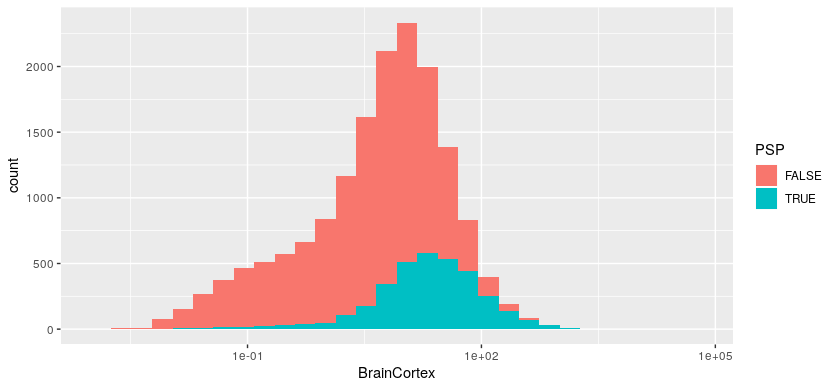
\includegraphics[width=\linewidth]{images/Rplot_corrected_gtex_histogram_log.png} 
%         \caption{Histogram of expression PSP and non PSP. Log10 scale} \label{fig:gtex_histogram_log}
%     \end{subfigure}
%     \hfill
%     \begin{subfigure}[t]{0.45\textwidth}
%         \centering
%         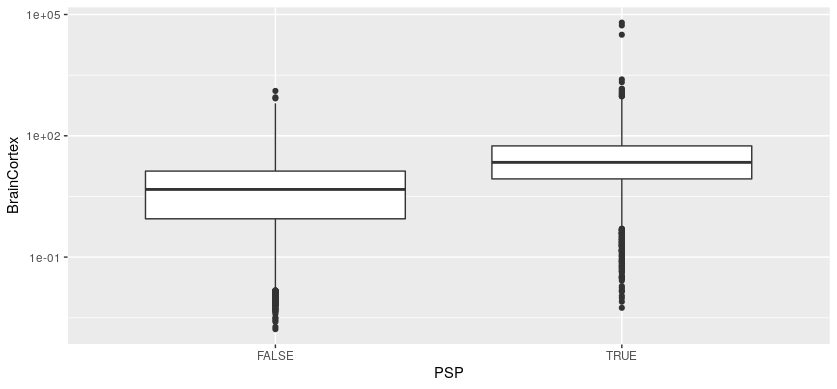
\includegraphics[width=\linewidth]{images/Rplot_corrected_gtex_boxplot_log10.png} 
%         \caption{Gtex expression boxplot PSP against not PSP. Log10 scale} \label{fig:gtex_log_boxplot}
%     \end{subfigure}
%     \caption{Plots of GTEx expression \textcolor{red}{may want to do this in subfigure packages rather than subcaption to line up edges and tidy up images in ggplot}}
%     \label{fig:all_gtex_panels}
% \end{figure}
\subsubsection{Correlation of GTEx expression across brain}

Table~\ref{tab:Correlation of PSP gene expression across brain regions. Expression values $log_2$ transformed with pseudocount of 1} shows correlation of expression of PSP genes between brain regions. Pearson product moment correlation. Anterior cingulate cortex (mean correlation 0.94) was the most correlated brain region and cerebellum the least (mean correlation 0.85). Minimum pairwise correlation cerebellar hemisphere and substantia nigra (0.792) max\footnote{code at \url{source('~/RProjects/gtex/R/graph_gtex/gtex_correlation_table.R')}} Highest (non identical) correlation caudate and putamen 0.996 (both basal ganglia). For all regions non identical  1st Quartile 0.839, Median 0.948, Mean 0.914, 3rd Quartile 0.9680, Max = 0.996).

PSP gene expression is correlated and lowest correlations are found in the cerebellar hemisphere as reported by Mele \cite{mele2015human} suggesting that the PSP group is a not markedly different from CNS expressed genes overall. \todo{paraphrase}

Expression for genes in the PSP but not in the consensus PSD used by Hill et al\cite{hill2014human} n=1323 \todo{Ref to Bayes SG paper although link to set in G2C is broken} is increased compared to the rest of the genome including the consensus genes. The consensus genes are more highly expressed than the PSP genes not in the consensus set but the effect is much more modest (see supplementary tables)\footnote{\url{source('~/RProjects/gtex/R/graph_gtex/gtex_correlation_table_hPSD_too.R')}}.

% latex table generated in R 3.6.3 by xtable 1.8-4 package
% Sat Aug  8 07:51:39 2020source('~/RProjects/paper_xls_output/R/chapter_2/FUMA/edit_gene_table/EA2_FUMA2clipboard.R')


\begin{table}[ht]
\centering
\begin{adjustbox}{width=\textwidth}

\begin{tabular}{lrrrrrrrrrrrr}
  \hline
 &   Amy &   ACC &   Cau &   Ce H &   Cer &   Cor &   FC  &   Hip &   Hyp &   NA &   Put &  SN \\ 
  \hline
  Amygdala & 1.00 & 0.98 & 0.97 & 0.80 & 0.81 & 0.96 & 0.95 & 0.99 & 0.97 & 0.97 & 0.97 & 0.95 \\ 
    Anterior cingulate cortex  & 0.98 & 1.00 & 0.96 & 0.83 & 0.83 & 0.99 & 0.99 & 0.97 & 0.96 & 0.97 & 0.95 & 0.91 \\ 
    Caudate$^*$ & 0.97 & 0.96 & 1.00 & 0.80 & 0.81 & 0.95 & 0.94 & 0.97 & 0.95 & 0.99 & 1.00 & 0.93 \\ 
    Cerebellar Hemisphere & 0.80 & 0.83 & 0.80 & 1.00 & 0.99 & 0.84 & 0.84 & 0.81 & 0.83 & 0.81 & 0.79 & 0.78 \\ 
    Cerebellum & 0.81 & 0.83 & 0.81 & 0.99 & 1.00 & 0.86 & 0.84 & 0.82 & 0.84 & 0.82 & 0.80 & 0.79 \\ 
    Cortex & 0.96 & 0.99 & 0.95 & 0.84 & 0.86 & 1.00 & 0.99 & 0.96 & 0.93 & 0.95 & 0.94 & 0.88 \\ 
    Frontal Cortex  & 0.95 & 0.99 & 0.94 & 0.84 & 0.84 & 0.99 & 1.00 & 0.95 & 0.94 & 0.95 & 0.93 & 0.88 \\ 
    Hippocampus & 0.99 & 0.97 & 0.97 & 0.81 & 0.82 & 0.96 & 0.95 & 1.00 & 0.97 & 0.96 & 0.97 & 0.95 \\ 
    Hypothalamus & 0.97 & 0.96 & 0.95 & 0.83 & 0.84 & 0.93 & 0.94 & 0.97 & 1.00 & 0.95 & 0.95 & 0.97 \\ 
    Nucleus accumbens$^*$ & 0.97 & 0.97 & 0.99 & 0.81 & 0.82 & 0.95 & 0.95 & 0.96 & 0.95 & 1.00 & 0.98 & 0.91 \\ 
    Putamen$^*$  & 0.97 & 0.95 & 1.00 & 0.79 & 0.80 & 0.94 & 0.93 & 0.97 & 0.95 & 0.98 & 1.00 & 0.94 \\ 
     Substantia nigra & 0.95 & 0.91 & 0.93 & 0.78 & 0.79 & 0.88 & 0.88 & 0.95 & 0.97 & 0.91 & 0.94 & 1.00 \\ 
   \hline
\end{tabular}
\end{adjustbox}
\caption[Correlation of PSP gene expression across brain regions]{Correlation of PSP gene expression across brain regions. Expression values $log_2$ transformed with pseudocount of 1. n=3055 genes passing quality control. *=basal ganglia. Frontal cortex = Brain area 9, Anterior cingulate cortex = 24.}
\label{tab:Correlation of PSP gene expression across brain regions. Expression values $log_2$ transformed with pseudocount of 1}
\end{table}




\section{Genome Wide Association Studies}

Previous network analyses have shown that synaptic topological models are differentially enriched for disease and gene ontology terms. There is also evidence that central nodes may be more likely to be disease nodes. These analyses have not however made use of the complex polygenetic signal available in genome wide association studies. Chapter 1 introduced the reasons for using intelligence as a phenotype.

To test the association between synaptic proteome network properties and structures and population genetic variation associated with intelligence we will need to calculate a statistic measuring the association of genetic variants with the phenotype for each gene that is represented by a node in the network. These values will be calculated using MAGMA in four samples, two of intelligence and two of educational attainment.\cite{de2015magma}
\todo[inline]{?add diagram of cohorts}

\subsection{Cohorts}
\label{sec:cohorts from paper section}
%\textcolor{red}{from paper section}
To investigate whether topological communities are enriched with genetic variants associated with cognitive ability and educational attainment and to reduce type II \footnote{This will reduce the number of tests to those that are likely to be true. 
or in the see section} error I will use a discovery and replication cohort design (see section~\ref{sec:Study design topology based GSA} and figure~\ref{fig:study design community detection}.) 
For consistency I will refer throughout the text to the GWA study of genetic variants associated with intelligence in UK Biobank\cite{bycroft2018uk} as Intelligence\textsubscript{Discovery} and the Phase II Educational attainment GWA study conducted using UK Biobank as Education\textsubscript{Discovery}.

We refer to the meta-analytic GWAS of intelligence carried out by Sniekers et al. from the Complex Trait Genetics (CTG) lab as Intelligence\textsubscript{Replication} \cite{sniekers2017genome}.   The meta-analysis of GWA studies of educational attainment excluding UK Biobank and 23andMe by Okbay et al.\cite{okbay2016genome} (often called EA2 - Educational Attainment 2) is referred to as Education\textsubscript{Replication}. Details of the generation and composition of these samples are found in section~\ref{sec:samples from paper section}. 

Two further samples became available after the completion of the primary analysis. These are the largest intelligence and education cohorts to date \cite{savage2018genome}, \cite{lee2018gene} but overlap with the samples above. They will be used to check the findings from earlier sections in chapter~\ref{chap:checking our findings} section~\ref{sec:placeholder for incoming refs chapter 5}

\subsection{Samples}

\label{sec:samples from paper section}
The information in this section is taken from that prepared by Dr Hill for a manuscript we are preparing. Dr Hill calculated the $\chi^2$ estimates of heritability. I have repeated these calculations using LD hub\footnote{LD hub \url{http://ldsc.broadinstitute.org/ldhub/} code to prepare files for LD hub at \url{source('~/RProjects/format_hub/R/format_summary_hub.R')}} a web interface for LD score regression \cite{zheng2017ld}.

 The Intelligence\textsubscript{Discovery} sample was formed using the ‘fluid’ cognitive test from UK Biobank; we shall refer to it as verbal-numerical reasoning (VNR). The VNR test contains 13 multiple choice items, six of which are verbal with the remaining seven being numerical in nature. Each individual’s VNR score was the sum of correct responses attained within a two-minute time period. This test has a large genetic correlation with intelligence scores derived from psycho-metrically validated cognitive tests \cite{hill2019combined}. A total of 120 934 participants (mean $\chi^2$=1.52) were available for analysis who did not contribute data to the Intelligence\textsubscript{Replication}\cite{sniekers2017genome} data set. A full description of how data from these participants was analysed can be found in Hill et al. \cite{hill2019combined}. 
 
UK Biobank was also used as the Education\textsubscript{Discovery} sample. Summary statistics were taken from Hill et al. on 273 274 participants (mean  $\chi^2$= 1.67).\footnote{redone by me  $\chi^2$=1.6684 see full results in errata folder verbatim for output} \cite{hill2019combined}  Education was defined as a binary choice of whether or not the individual had a University/College degree. A full description of how these data were analysed can be found in Hill et al. \cite{hill2019combined}.

The Intelligence\textsubscript{Replication} data set was formed using summary statistics obtained from the Sniekers et al. GWAS meta-analysis of intelligence (n = 78 308, mean $\chi^2$= 1.30).  \cite{sniekers2017genome}  An Education\textsubscript{Replication} data set was formed using summary GWAS data based on the the GWAS meta-analysis by Okbay et al (n = 217 569, mean $\chi^2$= 1.43) with UK Biobank participants excluded. \cite{okbay2016genome}. The summary statistics with UK Biobank removed were kindly provided by Dr Okbay and colleagues who generated the new summary statistics.    (See tables~\ref{tab:supplementary dh table 1 datasets} and \ref{tab:supplementary LD regression hill}). 
%\todo[inline]{convert these tables to latex DONE}
For genotype, meta-analysis methods and association analyses see the publications reporting the original GWAS\cite{sniekers2017genome}\cite{okbay2016genome}\cite{hill2019combined}.

%\textcolor{red}{end from paper section} \todo{add the calculation of chi sq for these studies was performed by Dr Hill in the course of preparation of a manuscript based on the community detection results}

%textcolor{red}{this is done using LD regression from LD hub repeat this yourself}
\todo{LD hub regression available at Broad sign in using google I have used grantsynch ref for LD hub in extras}

 

\todo{add the LD hub acknowledgements file to the acknowledgements: it is verbatim word formatted - in file verbatim.tex in folder errata}



\subsection{MAGMA Gene level statistics: Validation}
\label{sec:MAGMA Gene level statistics validation from other studies}

To ensure the accuracy of the gene level significance statistic I compared the gene level scores obtained using MAGMA to those reported in available studies\cite{de2015magma}. Potential sources of variation or bias include variations in command line options for software such as MAGMA,  different calculation of gene scores for raw genotype and summary data (see section~\ref{sec:MAGMA_gene_scores}) and different software versions, different reference populations to account for LD and variation in low level libraries across platforms\footnote{and there is the issue about performance across platforms}.\cite{kim2018experimenting} There were no published papers available containing a MAGMA gene-level analysis of the Intelligence\textsubscript{Discovery} sample or Education\textsubscript{Discovery}.\footnote{see discussion on benchmarking} 


The study by Okbay et al. (EA2)\cite{okbay2016genome}, providing the Education\textsubscript{Replication} sample did not report MAGMA gene scores, and differs from the Education\textsubscript{Replication} sample by including UK Biobank Educational attainment data. The only published reports of MAGMA gene scores from the exact discovery and replication samples was, therefore, the Intelligence\textsubscript{Discovery} sample \cite{sniekers2017genome}\footnote{no magma version in MS or supplemental online} \footnote{(supplementary table 8 at \url{https://static-content.springer.com/esm/art\%3A10.1038\%2Fng.3869/MediaObjects/41588_2017_BFng3869_MOESM2_ESM.xlsx})}.

We have, however, had access to the MTAG (Multi-trait analysis of Genome-Wide Summary data) summary data from the paper published by Hill, which contained MAGMA gene scores although it does contain data derived from educational attainment data so is not identical with the Intelligence\textsubscript{Discovery} sample\todo{need to check with David if it is ok to use this data it is for qc}. \footnote{no magma version in MS, none in supplementary material}\footnote{ sheet 5 at \url{https://static-content.springer.com/esm/art\%3A10.1038\%2Fs41380-017-0001-5/MediaObjects/41380_2017_1_MOESM2_ESM.xlsx}}\cite{hill2019combined}. One
can obtain a subset of the UK Biobank Education data which reports MAGMA scores for the top scoring 95 genes in the study by Davies et al. 2016 \cite{davies2016genome} \footnote{the MAGMA results for the top 95 genes are reported in the first sheet in Supplementary table 3A \url{https://static-content.springer.com/esm/art\%3A10.1038\%2Fmp.2016.45/MediaObjects/41380_2016_BFmp201645_MOESM506_ESM.xls}}. The MAGMA version is not recorded. Phase 1, release 3 of 1000 Genomes was used (in contrast to phase 3 for present study.\todo{ask Douglas should we store these and have a data provenance subchapter}. Finally  summary data has recently been made available from the current largest GWAS of intelligence to date by Savage et al. \cite{savage2018genome} ($n=269 867$) this reports MAGMA Gene level analysis results although only for significant genes\todo{check} \footnote{ (table S15 in supplementary materials at \url{https://www.ncbi.nlm.nih.gov/pmc/articles/PMC6411041/bin/NIHMS1006639-supplement-Supplementary_Tables.xlsx})}.

The pairwise correlation between the gene scores reported in these studies and the results I calculated using MAGMA and their summary statistics  are shown in table~\ref{tab:Correlation between MAGMA gene scores obtained from summary statistics and those published in supplementary material to papers}. Magma 1.06b for MacOS was used with 1000 Genomes Phase 3 data to account for linkage disequilibrium. NCBI 37 was used for gene boundaries.\todo{? remove the Davies one was only 93 genes and older now}\todo{codepath} Summary GWAS statistics were used to calculate gene scores using default settings. No gene window was used.\footnote{they used one in savage but only 5kB}

\begin{table}[ht]
    \centering
    
    \begin{tabular}{llllllll}
    \toprule
        Study & n & t & df & p & Pearson & CI   \\
        \midrule
       Savage \cite{savage2018genome} & 269687 & 122.26& 352  & $<2.2 \times 10^{-16}$ & 0.99 & 0.986-0.991  \\ 
       Hill \cite{hill2019combined} & 248482 & 368.27 & 17475 & $<2.2 \times 10^{-16}$& 0.94 & 0.939-0.942 \\
       Davies (2016) \cite{davies2016genome} & 112151 & 22.08 & 93 & $<2.2 \times 10^{-16}$ & 0.92 & 0.88-0.94\\
       Sniekers \cite{sniekers2017genome}& 78308 & 466.41 & 18246 & $<2.2 \times 10^{-16}$ & 0.96 & 0.959-0.962\\
       \bottomrule
    \end{tabular}
    \caption{Correlation between MAGMA gene scores obtained from summary statistics and those published in supplementary material to papers.}
    \label{tab:Correlation between MAGMA gene scores obtained from summary statistics and those published in supplementary material to papers}
\end{table}

\subsubsection{Results}
The correlation coefficient varied in the range 0.92-0.99 despite slight differences in software version, gene windows and the potential use of genotyped versus summary data. I conclude that apart from small variants that there is no systematic inaccuracy in the calculation of MAGMA gene scores using the plaform and pipeline. 

The MAGMA versions were not documented in Sniekers et al., Davies et al or Hill et al. \cite{davies2016genome} or \cite{sniekers2017genome} \cite{hill2019combined}. 1000 Genomes phase 1 data was used in Davies et al.\cite{davies2016genome}. 

\subsection{Synaptic genes omitted from NCBI 37}
\todo[inline]{should this be earlier}
The studies from which we obtained summary statistics used NCBI 37 to provide gene boundaries in MAGMA. Seventeen of the PSP genes were not in the reference NCBI 37 boundaries text file supplied with MAGMA used to assign SNPs to genes in MAGMA. Files containing NCBI 36,37 and 38 boundaries are supplied on the MAGMA project website,  5 of the genes not in the NCBI37 file have boundaries defined in the NCBI 38 and are shown in table~\ref{tab:Synaptic PSP genes  found in NCBI 38 but not in 37 listing included with MAGMA}\footnote{code \url{source('~/RProjects/annotations_phd/R/missing_NCBI_genes.R')}}.

10 genes are found in neither the NCBI 37 nor the NCBI 38 gene boundary files but are annotated in the\textit{ homo sapiens} gene info download in Entrez Gene at the NCBI\footnote{Link at \url{https://ftp.ncbi.nih.gov/gene/DATA/GENE_INFO/Mammalia/Homo_sapiens.gene_info.gz} }\todo{date of file}. The annotations of the 10 synaptic genes (not in the NCBI 38 file included with MAGMA) but present in NCBI Entrez Gene info\footnote{\url{ftp://ftp.ncbi.nih.gov/gene/}} are shown in table~\ref{tab:10 synaptic genes not in NCBI 38 included with MAGMA but present in entrez gene gene info}.

Two pseudo genes were identified using the ToppGene API\cite{chen2009toppgene}: Entrez id:	441400, RAB1C, member RAS oncogene family pseudogene UniProt Q92928 Protein transport. Probably involved in vesicular traffic (By similarity); Entrez id:	440915	,POTEKP\footnote{POTE expressed in Prostate ovary testis and placenta}, POTE ankyrin domain family member K, pseudogene \cite{bera2002pote} Uniprot Putative beta-actin-like protein 3 Q9BYX7. 


Gene ontology enrichment analysis using ToppFun (part of the ToppGene suite) (see section~\ref{sec:ToppGene GO erncihement}) did not find any phenotype or ontology suggestive of being associated with cognition in particular no human or murine phenotype (GO:0034987	immunoglobulin receptor binding 	p Bonferroni $6.224\times10^{-9}$	6 terms, 	GO:0097478	leaflet of membrane bilayer	Bonferroni p	$1.296\times10^{-3}$	6	terms. The only potentially concerning term is 23380,	SRGAP2	SLIT-ROBO Rho GTPase activating protein 2 which is associated with the cellular component dendritic spine head GO:0044327 and associated with neural morphogenesis\cite{guerrier2009f}. The gene list was also analysed using the Gene2Func interface in FUMA \cite{watanabe2017functional} (see section~\ref{sec:FUMA go enrichment}). In particular there were no enriched gene sets and no hits in GWAS catalog\footnote{sic}\cite{welter2014nhgri}.

 While it would be possible to make a custom annotation file for these genes this would complicate our analysis and cause it to differ methodologically from other analyses reporting gene level statistics in MAGMA.  \footnote{note to Douglas: i am probably not explaining this well but what I am trying to say is that they don't look important, it makes our analysis different from anybody elses and there is also a where do you stop problem and also you could argue a need for further correction for multiple testing if you are modifying standard testing procedures Reporting it may seem a bit over the top but it is part of the QC we have done - comparing magma to vegas, magma to pascal, two gsa methods, two gene score methods, compare significant genes for any commonalities}  
% latex table generated in R 3.6.1 by xtable 1.8-4 package
% Wed Feb 19 14:14:05 2020
% latex table generated in R 3.6.1 by xtable 1.8-4 package
% Wed Feb 19 14:15:51 2020
\begin{table}[ht]
\centering
\begin{adjustbox}{max width=\textwidth}
\begin{tabular}{cclll}
  \hline
 Gene ID & Symbol & chromosome & type of gene & Full name from nomenclature authority \\ 
  \hline
1804 & DPP6 & 7 & protein-coding & dipeptidyl peptidase like 6 \\ 
  3635 & INPP5D & 2 & protein-coding & inositol polyphosphate-5-phosphatase D \\ 
  3800 & KIF5C & 2 & protein-coding & kinesin family member 5C \\ 
  9554 & SEC22B & 1 & protein-coding & SEC22 homolog B, vesicle trafficking protein (gene/pseudogene) \\ 
  23380 & SRGAP2 & 1 & protein-coding & SLIT-ROBO Rho GTPase activating protein 2 \\ 
   \hline
\end{tabular}
\end{adjustbox}
\caption[Synaptic PSP genes with boundaries found only in NCBI 38]{Synaptic PSP genes  found in NCBI 38 gene boundary file supplied with MAGMA but not in NCBI 37 file. Gene ID = Entrez Gene Gene ID.}
\label{tab:Synaptic PSP genes  found in NCBI 38 but not in 37 listing included with MAGMA}
\end{table}
   


\begin{table}[ht]
\centering
\begin{adjustbox}{max width=\textwidth}
\begin{tabular}{clcll}
  \hline
 Gene ID & Symbol & chromosome & type of gene & Full name from nomenclature authority \\ 
  \hline
293 & SLC25A6 & X$|$Y & protein-coding & solute carrier family 25 member 6 \\ 
  3493 & IGHA1 & 14 & other & immunoglobulin heavy constant alpha 1 \\ 
  3500 & IGHG1 & 14 & other & immunoglobulin heavy constant gamma 1 (G1m marker) \\ 
  3502 & IGHG3 & 14 & other & immunoglobulin heavy constant gamma 3 (G3m marker) \\ 
  3503 & IGHG4 & 14 & other & immunoglobulin heavy constant gamma 4 (G4m marker) \\ 
  3507 & IGHM & 14 & other & immunoglobulin heavy constant mu \\ 
  3514 & IGKC & 2 & other & immunoglobulin kappa constant \\ 
  4509 & ATP8 & MT & protein-coding & mitochondrially encoded ATP synthase 8 \\ 
  4513 & COX2 & MT & protein-coding & mitochondrially encoded cytochrome c oxidase II \\ 
  4538 & ND4 & MT & protein-coding & mitochondrially encoded NADH dehydrogenase 4 \\ 
   \hline
\end{tabular}
\end{adjustbox}
\caption[Synaptic genes not in NCBI boundary files in MAGMA]{10 synaptic genes not in NCBI gene boundary files (NCBI36,37,38) included with MAGMA but present in Entrez Gene Homo sapiens gene info files \url{https://ftp.ncbi.nih.gov/gene/DATA/GENE_INFO/Mammalia/Homo_sapiens.gene_info.gz}.  GeneID, NCBI Entrez Gene GeneID }
\label{tab:10 synaptic genes not in NCBI 38 included with MAGMA but present in entrez gene gene info}
\end{table}

\section{MAGMA gene level statistic methods}
\label{sec:MAGMA gene level methods}
MAGMA version 1.06 for MacOS was used with 1000 Genome European Ancestry Phase 3 data to account for linkage disequilibrium\footnote{\url{https://ctg.cncr.nl/software/MAGMA/ref_data/g1000_eur.zip}}1000 Genomes phase 3 data of European ancestry and NCBI 37 data provided on the MAGMA website \footnote{\url{https://ctg.cncr.nl/software/MAGMA/aux_files/NCBI37.3.zip}} was used to define gene boundaries. Output logs are included in the supplemental material.  Command line arguments were supplied using a bash shell script and default settings were used for summary GWAS statistic data (SNPwise sum). \footnote{these will be moving to github - this might be too much most papers just say what I have said above -  \url{/Users/grantrobertson/Programs/copy_paperMagma_draft-master/magma_script.sh}	}

Gene level statistics were calculated and no window was used around gene boundaries (see section~\ref{sec:Gene windows} below). In studies where the number of individuals tested per SNP was available in the summary data this was supplied as a command line argument - otherwise the overall sample size was used. SNPs that were analysed in less than 50 individuals were discarded (default setting). 

\subsubsection{Gene Windows}
\label{sec:Gene windows}
\todo[inline]{? comes before}
 In order to include gene regulatory elements in gene level analysis a number of ``windows"%WYN
around the gene boundary have been used, both symmetric and asymmetric. VEGAS \cite{liu2010versatile} used a set 50kB boundary and this is incorporated in studies that used this method (e.g Hill et al. (2014)\cite{hill2014human})

The use of a gene window significantly affects the number of SNPs assigned to genes.  Using the College Phenotype from Rietveld et al. \cite{rietveld2013gwas} and NCBI 37 gene boundaries 914887 SNPs were mapped to genes (39.45\% of 2319112 SNPs) using no window; with a 50kb window 1385602 (59.75\%) mapped to genes.\todo{? use other}
%WYN
The reported window sizes vary. Zhao and Nyholt \cite{zhao2017gene} in a study of gene level statistics across psychiatric disorders using the GATES method \cite{li2011gates}  used a 15kb window reasoning that 90\% \cite{pickrell2010understanding} of eQTL are found in this region. 

The predominant practice at present appears to be either not use a gene window or only to use a small one (for example 5kb as reported in Savage et al (2018. \cite{savage2018genome}). In the absence of a widely agreed upon window size I have not used one believing this to be the simplest and most conservative option\footnote{especially as this is in part a proof of concept analysis and I don't want to get tied up in arguments about why I used window size a or b see previous footnote}. 


\begin{table}[]
    \centering
   
    \begin{tabular}{l|llll}
\toprule
    &  Intelligence\textsubscript{Replication}   & Education\textsubscript{Replication} &
    Intelligence\textsubscript{Discovery} & Education\textsubscript{Discovery} \\
    \midrule
     Intelligence\textsubscript{Replication}    & & 0.249 &0.378  & 0.308 \\
     Education\textsubscript{Replication} &0.249 &&0.325&0.506 \\
     Intelligence\textsubscript{Discovery}&0.378 &0.325&&0.446 \\
     Education\textsubscript{Discovery}&0.308&0.506 &0.446 & \\
\bottomrule
    \end{tabular}
    \caption[Correlation of MAGMA GWGAS scores between samples]{Correlation of MAGMA GWGAS scores between samples. Pearson product moment correlation. p$<2.2\times10^{-16}$ all tests. Correlation is between $-log10(p)$ transformation of gene level p values. Cases where a gene score is present in one study and not another are ignored}
    \label{tab:correlation of MAGMA GWGAS scores}
\end{table}

\subsection{Correlation MAGMA GWGAS}
\todo[inline]{cant have this before introduction of cohorts}
Educational attainment and Intelligence are genetically correlated\cite{plomin2018new} (see table~\ref{tab:LD regression hill}). It is likely that gene level scores in samples between and within these phenotypes are also correlated although this should be less than the overall SNP correlation due to inter-genic SNPs and and loss of information in the aggregation of SNPs to genes. It is worthwhile checking that the value is not extreme or unexpected (for example higher between low powered samples with different phenotypes) as part of overall quality control. 


Correlation was calculated between the -log10 transform of gene level p values between samples using Pearsons product moment correlation test in R. Where a gene did not have a p value in a study this pairwise comparison was omitted. I have calculated MAGMA GWGAS gene level correlation rather than genetic correlation because we will be using MAGMA GWGAS statistics to make comparisons of the effect of central nodes across samples. The correlation is greatest between the two educational attainment samples (0.506; CI 0.495-0.516, t = 78.473, df = 17928, p-value $< 2.2 \times 10^{-16}$) (table~\ref{tab:correlation of MAGMA GWGAS scores}). For each sample other than Intelligence\textsubscript{Discovery} the correlation is highest with the matching phenotype and Intelligence\textsubscript{Replication} is still most highly correlated with Intelligence\textsubscript{Discovery}. The two discovery samples are similar in composition and the Intelligence\textsubscript{Replication} sample is likely to be the least power (lowest sample size, meta-analysis and lowest $\chi^2$ on testing heritability using LD score regression (section~\ref{sec:samples from paper section}). 
\footnote{REMOVE FINAL: Result details commented out search \%DETAILS in tex} \footnote{\url{source('~/RProjects/paper_xls_output/R/chapter_2/MAGMA/pairwise_gene_comparison.R')}}
%%%%% COMPARE DETAILS
% t = 34.404, df = 17937, p-value < 2.2e-16
% alternative hypothesis: true correlation is not equal to 0
% 95 percent confidence interval:
%  0.2350242 0.2624803
% sample estimates:
%       cor 
% 0.2488022 

% ed and ctg

% 	Pearson's product-moment correlation

% t = 43.632, df = 18158, p-value < 2.2e-16
% alternative hypothesis: true correlation is not equal to 0
% 95 percent confidence interval:
%  0.2948248 0.3211538
% sample estimates:
%       cor 
% 0.3080483 


% 	Pearson's product-moment correlation

% ukbb int and ctg
% t = 55.029, df = 18158, p-value < 2.2e-16
% alternative hypothesis: true correlation is not equal to 0
% 95 percent confidence interval:
%  0.3655291 0.3904609
% sample estimates:
%       cor 
% 0.3780636 

% 	Pearson's product-moment correlation

% ukbbed and ctg
% t = 43.632, df = 18158, p-value < 2.2e-16
% alternative hypothesis: true correlation is not equal to 0
% 95 percent confidence interval:
%  0.2948248 0.3211538
% sample estimates:
%       cor 
% 0.3080483 


% ukbbint and ea2
% 	Pearson's product-moment correlation

% 	Pearson's product-moment correlation

% t = 46.068, df = 17928, p-value < 2.2e-16
% alternative hypothesis: true correlation is not equal to 0
% 95 percent confidence interval:
%  0.3121876 0.3383644
% sample estimates:
%       cor 
% 0.3253383  
% 	Pearson's product-moment correlation
% ed and ea2

% t = 78.473, df = 17928, p-value < 2.2e-16
% alternative hypothesis: true correlation is not equal to 0
% 95 percent confidence interval:
%  0.4946612 0.5164525
% sample estimates:
%       cor 
% 0.5056375 

% 	Pearson's product-moment correlation

% ed and int  
% t = 67.416, df = 18285, p-value < 2.2e-16
% alternative hypothesis: true correlation is not equal to 0
% 95 percent confidence interval:
%  0.4344972 0.4577150
% sample estimates:
%       cor 
% 0.4461812 

\begin{table}[]
    \centering
    \begin{tabular}{lllll}
    \toprule
        Phenotype & n & mean $\chi^2$ & LD intercept (SE) & Reference \\
        \midrule
        Intelligence & 78308 & 1.30 & 1.02(0.01) & Sniekers et al.(2017)\cite{sniekers2017genome}\\
        &120934 & 1.53 & 1.02 (0.01)& NA\\
        \\
        Education&273274 & 1.67 & 1.042(0.01) & NA\\
         & 217569&1.43&1.02(0.01) & Okbay et al.(2016)\cite{okbay2016genome}\\
         \bottomrule
    \end{tabular}
    \caption[Summary for each data set]{References and heritability of each data set. Table adapted from table generated by W.D Hill for publication. Calculations and arrangement are work of Dr W.D. Hill}
    \label{tab:supplementary dh table 1 datasets}
\end{table}



\begin{table}[]
    \centering
    \begin{tabular}{l|lllll}
    \toprule
       Phenotype & Samples & Intelligence & & Education &    \\
       \midrule
         & & Hill & Sniekers & Okbay & Hill\\
         \midrule
         Intelligence & Hill & 21.19\%(0.91\%) & & & \\
         & Sniekers & 0.99(0.02) & 19.45\%(1.09) & & \\
         \\
         Education & Okbay & 0.62(0.03) & 0.75(0.02) & 9.78(0.44\%) &\\
         & Hill & 0.66(0.02) & 0.72(0.02) & 0.96(0.02)&11.67\%(0.91\%)\\
         \bottomrule
    \end{tabular}
    \caption[Heritability of samples]{Using LD score regression heritability within, and genetic correlations between, each of the data sets used is shown. Heritability on the observed scale is shown on the diagonal and genetic correlations are shown on the off diagonal with standard error in brackets. Table contents and caption from WD Hill. }
    \label{tab:supplementary LD regression hill}
\end{table}
\subsection{Intelligence\textsubscript{Replication} GWGAS}
\label{sec:Intelligence Replication GWGAS}

\subsubsection{Methods}
The Intelligence\textsubscript{Replication} sample is identical to the individuals in the 2017 ``Intelligence wave 1" meta-analysis study by Sniekers et al. \cite{sniekers2017genome} (see table~\ref{tab:supplementary dh table 1 datasets}. 

GWAS summary data were downloaded from the Complex Trait Genomics (CTG) lab\footnote{ \url{https://ctg.cncr.nl/documents/p1651/sumstats.txt.gz}}. This meta-analysis of 78,308 individuals was derived from 13 cohorts. 29,610 individuals were reported for the first time. UK Biobank participants had either taken a web based test ($n=17852$, raw genotype data used, reported for first time) or touch screen test ($n=35257$). 12441 participants were from the CHIC consortium used to produce an GWAS of childhood intelligence\cite{benyamin2014childhood}. 5 additional cohorts contributed $n=11 749$ participants. The individuals making up this meta-analysis do not contribute to any of the other three samples used in this thesis: individuals from UK Biobank were excluded from the Intelligence\textsubscript{Discovery} sample summary statistics provided by Dr Hill\footnote{see contributors/acknowledgments}. The authors report finding 47 genome wide significant genes using MAGMA to perform a Genome Wide Gene Association (GWGAS)\cite{sniekers2017genome},\cite{de2015magma}.

Gene level scores were calculated using MAGMA v1.6b (Mac OS)(section~\ref{sec:MAGMA gene level methods}) \footnote{Code to produce the following tables is at \url{source('~/RProjects/paper_xls_output/R/0_write_MAGMA_gene_level_results_PhD.R')} }. The number of individuals tested for each SNP was available and used for sample size. The European panel of the 1000 Genomes Phase 3 was used to account for linkage disequilibrium
 updated 19/09/2018 downloaded from CTG MAGMA website \footnote{\url{https://ctg.cncr.nl/software/magma}}. SNPs were assigned to genes using NCBI37.3 Gene Boundaries from the CTG website.  No window was used around gene boundaries. Default options for summary stastics were used (SNPwise). For all subsequent GWGAS performed using MAGMA methods are identical unless otherwise stated. 
% Welcome to MAGMA v1.06b (mac)

% Using flags:
%         --bfile g1000_eur
%         --gene-annot ./annotations/annotated_bim.genes.annot
%         --pval /Users/grantrobertson/Programs/GWAS_studydata/sumstats.txt use=3,11 ncol=6
%         --out ./gene_results/ctg

% Start time is 11:28:37, Wednesday 12 Sep 2018

% Loading PLINK-format data... 
% Reading file g1000_eur.fam... 503 individuals read
% Reading file g1000_eur.bim... 22665064 SNPs read
% Preparing file g1000_eur.bed... 

% Reading SNP synonyms from file g1000_eur.synonyms (auto-detected)
%         read 5966573 synonyms from file mapping to 3894269 SNPs in the data
%         WARNING: detected 102 synonymous SNP pairs in the data
%                  skipped all synonym entries involved, synonymous SNPs are kept in analysis
%                  writing list of detected synonyms in data to supp lementary log file
% Reading SNP p-values from file /Users/grantrobertson/Programs/GWAS_studydata/sumstats.txt... 
%         detected 12 variables in file
%         using variable: rsid (SNP id)
%         using variable: p_value (p-value)
%         using variable: N (sample size; discarding SNPs with N < 50)
%         read 12104295 lines from file, containing valid SNP p-values for 10674310 SNPs in data (88.19% of lines, 47.1% of SNPs in data)
%         WARNING: file contained 3 duplicate SNPs (same IDs or synonyms)
%                  dropped all occurrences of each from analysis
%                  writing list of duplicated IDs to supplementary log file
% Filtering phenotype/covariate missing values... 503 individuals remaining

% Loading gene annotation from file ./annotations/annotated_bim.genes.annot... 
%         19248 gene definitions read from file
%         found 18262 genes containing SNPs in genotype data

% Starting gene analysis... 
%         using model: SNPwise-sum

%         writing gene analysis results to file ./gene_results/ctg.genes.out
%         writing intermediate output to file ./gene_results/ctg.genes.raw


% End time is 11:40:04, Wednesday 12 Sep 2018 (elapsed: 00:11:27)


\subsubsection{Results}
18262\footnote{19427 genes in NCBI 37} genes were assigned gene level p values using MAGMA v1.06.
The Bonferroni correction for multiple comparisons was used to calculate a genome wide significance level ($\alpha$ = 0.05/18262; p=$2.74 \times 10^{-06}$). 47 genes achieved genome wide significance using the adjusted $\alpha$ level using MAGMA GWGAS (Genome Wide Gene Association Study) using the summary statistics provided. This is identical to the number reported by Sniekers et al. \cite{sniekers2017genome}. 16 of these were found in the PSP (34.0\%)  (table~\ref{tab:significant genes}).\footnote{Code for Gene level statistics at \url{source('~/RProjects/paper_xls_output/R/0_write_MAGMA_gene_level_results.R')}}. \footnote{Only 7 significant genes were found in the 1312 gene consensus PSD network graph\cite{mclean2016improved}}. 

All significant genes are shown in table \ref{tab:Significant genes in ctg MAGMA GWAS} and significant synaptic genes are shown in table~\ref{tab:Significant synaptic genes in ctg MAGMA GWAS2} \footnote{Remove: tables complete on full compile}.

\begin{table}[ht]
    \centering
    \begin{tabular}{cccc}
    \toprule
         Study & n significant synaptic genes & n  significant genes & percent (\%) in PSP \\
      \midrule  
         Intelligence\textsubscript{Replication}\cite{sniekers2017genome} & 16 (7) & 47 & 34.0 \\
         Education\textsubscript{Replication}\cite{okbay2016genome} & 25(12) & 99 & 25.2 \\
         Intelligence\textsubscript{Discovery}\cite{hill2019combined} & 51 (17) & 196 & 26.0\\
         Education\textsubscript{Discovery}\cite{hill2019combined} & 58 (27) & 235 & 24.7\\
         \bottomrule
    \end{tabular}
    
    \caption[Number of Genome wide significant genes and number of genes in PSP at GWGAS in Intelligence and Educational Attainment samples]{Number of genome wide significant genes (using Bonferroni correction of 0.05/$n$ genes)   using MAGMA Genome Wide Gene Association Analysis Study (GWGAS) for Educational attainment and Intelligence discovery and replication samples. The references in the study column refer to the publication from which the majority of the sample are taken. Code to add core at \url{source('~/RProjects/paper_xls_output/R/chapter_2/exploratory_data_analysis_core_PSD.R')}. Number in parenthesis are number of significant genes in 1312 gene consensus hPSD.}
    \label{tab:significant genes}
\end{table}

% latex table generated in R 3.6.2 by xtable 1.8-4 package
% Thu Jan  2 13:21:27 2020

% latex table generated in R 3.6.1 by xtable 1.8-4 package
% Wed Feb 19 11:25:28 2020
\begin{table}[ht]
\centering
\begin{tabular}{llcrrc}
  \hline
 GeneID & Symbol & chromosome & $n$ SNPs & Z statistic & $p$ \\ 
  \hline
1434 & CSE1L &  20 & 176 & 5.96 & $1.26 \times 10^{-9}$ \\ 
  60412 & EXOC4 &   7 & 2184 & 5.88 & $1.99 \times 10^{-9}$ \\ 
  55964 & SEPT3 &  22 &  69 & 5.75 & $4.35 \times 10^{-9}$ \\ 
  6138 & RPL15 &   3 &  19 & 5.40 & $3.35 \times 10^{-8}$ \\ 
  23109 & DDN &  12 &   8 & 5.35 & $4.41 \times 10^{-8}$ \\ 
  85358 & SHANK3 &  22 & 199 & 5.31 & $5.49 \times 10^{-8}$ \\ 
  487 & ATP2A1 &  16 &  47 & 5.23 & $8.37 \times 10^{-8}$ \\ 
  11273 & ATXN2L &  16 &  36 & 5.17 & $1.17 \times 10^{-7}$ \\ 
  2870 & GRK6 &   5 &  39 & 5.07 & $2.03 \times 10^{-7}$ \\ 
  28512 & NKIRAS1 &   3 &  73 & 5.04 & $2.29 \times 10^{-7}$ \\ 
  4700 & NDUFA6 &  22 &  16 & 5.04 & $2.32 \times 10^{-7}$ \\ 
  
  4733 & DRG1 &  22 &  99 & 4.83 & $6.91 \times 10^{-7}$ \\ 
  10564 & ARFGEF2 &  20 & 406 & 4.80 & $7.83 \times 10^{-7}$ \\ 
  7284 & TUFM &  16 &   7 & 4.79 & $8.49 \times 10^{-7}$ \\ 
  553115 & PEF1 &   1 &  30 & 4.77 & $9.17 \times 10^{-7}$ \\ 
  8411 & EEA1 &  12 & 475 & 4.61 & $2.03 \times 10^{-6}$ \\ 
   \hline
\end{tabular}
\caption[Intelligence\textsubscript{Replication} Sample Genes in the PSP meeting genome wide significance levels for MAGMA GWGAS] { Intelligence\textsubscript{Replication} PSP synaptic Genes meeting genome wide significant at GWGAS using MAGMA for the Intelligence\textsubscript{Replication} sample. 16 genes are found in the PSP (34.0\%), Bonferroni corrected $\alpha=2.74 \times 10^{-06}$. $n$ SNPs = number of SNPs found within NCBI 37 
defined gene boundaries in sample. GeneID refers to Entrez Gene GeneID.} 
\label{tab:Significant synaptic genes in ctg MAGMA GWAS2}
\end{table}



\subsection{Education\textsubscript{Replication}  MAGMA GWGAS}
\label{sec:Edcuation replication gwgas}
\subsubsection{Methods}

The summary statistics for Education\textsubscript{Replication} are generated using individuals taken from the EA2 (Educational Attainment 2) meta-analytic GWA study of educational attainment\cite{okbay2016genome} with educational attainment defined as number of years of schooling completed.  The published study is of 293,723 individuals with 111,349 independent samples from UK Biobank used for out of sample replication \cite{sudlow2015uk}. A combined meta-analysis was carried out using the discovery and replication cohorts ($n$=405702) allowing an increase in the number of genome wide loci reported from 74 to 162. Due to Institutional Review Board (IRB) restrictions, which did not allow reporting of over 10,000 SNPs in the summary statistics for participants from 23andme, the summary statistics provided on the SSGAC website are of $n$=328917 individuals excluding 76155 individuals from 23andme\footnote{\url{http://ssgac.org/documents/EduYears_Main.txt.gz}}. The authors kindly made summary statistics available to us (see acknowledgements)\todo{cross ref to acknowledgements} excluding both 23andme and UK Biobank creating a sample that does not overlap with Education\textsubscript{Discovery}; $n$= 217568 (293723 - 76155 = 217568)\cite{okbay2016genome}.\footnote{See Okbay et al. supplemental information \url{http://ssgac.org/documents/SI_74_loci_educational_attainment.pdf} p 16} The summary statistics used were unsorted by sex. The modified summary statistics excluding UK Biobank and 23andMe  are deposited with the University of Edinburgh Research Data Service \footnote{https://www.ed.ac.uk/information-services/research-support/research-data-service}.
The number of individuals tested for each SNP was available and used. 20 duplicate SNPs were identified. 

\subsubsection{Results}



17942 genes were assigned a significance score using MAGMA 1.06 based on the SNP's present in the summary statistics.The Bonferroni correction for multiple comparisons was used to calculate a genome wide significance level ($\alpha$ = 0.05/17942; p=$2.79 \times 10^{-06}$). With this $\alpha$ level 99 genes were identified of genome wide significance. 25 (25.3\%) of these were found in the synaptic PSP (see table~\ref{tab:significant genes}).

Genome wide significant genes  are shown in table \ref{tab:Significant genes in EA2 MAGMA GWAS}, significant synaptic genes are shown in table \ref{tab:Significant synaptic genes in EA2  MAGMA GWAS}

% latex table generated in R 3.6.2 by xtable 1.8-4 package
% Thu Jan  2 13:31:54 2020






\subsection{Intelligence Discovery Phase II GWGAS}

\subsubsection{Methods}
The GWAS summary statistics for the Intelligence\textsubscript{Discovery} sample are taken from UK Biobank Phase II used as a part of an analysis by Hill et al.\cite{hill2019combined}. The authors used MTAG (Multi-Trait Analysis of GWAS) a technique that allows meta-analyses to increase their effective sample size using genetically related traits \cite{turley2018multi}. The published meta-analysis\cite{hill2019combined} combines the Intelligence\textsubscript{Replication} sample data \cite{sniekers2017genome} and UK Biobank Intelligence Phase II (Intelligence\textsubscript{Discovery} sample) combined with the genetically related educational attainment phenotype (the SSGAC EA2 study)\cite{okbay2016genome}. Summary GWAS statistics including only participants in UK Biobank Intelligence Phase II ($n$=120 934) were obtained from the Centre for Cognitive Ageing and Cognitive Epidemiology (CCACE) from the author Dr W.D. Hill.  A column is provided with the summary data of numbers tested per SNP but is constant and equal to the sample size and was used as the input for the GWGAS.      These subjects had taken the VNR test in UK Biobank which is closely related to intelligence \cite{hill2019combined}. For further details on the cohorts, genotyping and testing see Hill et al. \cite{hill2019combined}.


\subsubsection{Results}
18,287\footnote{ Was a to do - check as this is the same number as intelligence - i have checked and done diff on output logs they are different it may be they because they both came from David they used the same imputation and reported the same SNPs (they were done for the same study). The output otherwise is different} genes were assigned gene level statistics using MAGMA v1.06 to provide GWGAS.  With a Bonferroni $\alpha$ level of  $
2.73\times 10^{-06}$, 196\footnote{checked} genome wide significant genes were found at GWGAS using MAGMA. Of these 51 genes were in the PSP synaptic set (26.0\% of total) see table~\ref{tab:significant genes}.

Significant genes at the adjusted $\alpha$ level are shown in table \ref{tab:Significant synaptic genes in UKBB int  MAGMA GWAS}, significant synaptic genes are shown in table \ref{tab:Significant genes in UKBB int MAGMA GWAS}







\subsection{Education\textsubscript{Discovery} sample GWGAS}
\label{sec:UKBB Education discovery GWGAS}
\subsubsection{Methods}
The GWAS summary statistics for the Education\textsubscript{Discovery} Phase II are taken from UK Biobank Phase II. The data were obtained from the Centre for Cognitive Ageing and Cognitive Epidemiology (CCACE) from Dr W.D Hill (see acknowledgements). The sample size is $n$=273 274. The outcome measure is the achievement of a college or university degree which has been shown to correlated closely with years of education\cite{rietveld2013gwas}\todo{check ref}.

\subsubsection{Results}
18,287 genes contained SNPs. Numbers of individuals tested for each SNP were available and used in the command line argument. At a Bonferroni adjusted $\alpha$ level of $2.73 \times 10^{-06}$, 235 significant genes were identified. Of these, 58 were members of the PSP (24.7\%).  

Significant genes at alpha Bonferroni level are shown in table \ref{tab:Significant genes in UKBB edu MAGMA GWAS}, significant synaptic genes are shown in table \ref{tab:Significant synaptic genes in UKBB edu  MAGMA GWAS}\footnote{remove:cross ref correct when compiling all}.

% latex table generated in R 3.6.1 by xtable 1.8-4 package
% Fri Feb 21 12:10:53 2020
% latex table generated in R 3.6.2 by xtable 1.8-4 package
% Thu Jan  2 13:49:56 2020

\subsection{PASCAL and MAGMA}
Due to the centrality of the calculation of gene level p values to the investigation of the role of network structure, in cognitive ability and the significance of network structures I have used two different popular methods to calculate gene level p values for summary GWA data. PASCAL\footnote{version 0.1 15April 2016} uses methods similar to the popular VEGAS package and is discussed in more detail in section~\ref{sec:PASCAL community detection} \cite{lamparter2016fast} . There is a strong linear correlation between MAGMA gene level statistics and those calculated using PASCAL see table~\ref{tab:correlation MAGMA and PASCAL}. 

\subsubsection{PASCAL software}
The PASCAL software was used using the default options and no gene boundary. The empirical method was used for calculating $p$ values. No window was used around the gene boundaries defined using NCBI 37. 1000 Genomes Phase 3 was used to account for linkage disequilibrium. The sole release version  Alpha 0.1 was used and instructions were recorded as a shell script. \footnote{check above. In addition I have checked software version including on github site for project} 


%%% Table comparison of MAGMA and PASCAL %%%
\begin{table}[ht]
    \centering
    \begin{tabular}{lllccc}
    \toprule
    Sample & t & df & CI & cor & p \\
    \midrule
      Education\textsubscript{Discovery}   & 274.9 & 17241 & 0.890 - 0.905 & 0.902 & $<2.2 \times 10^{-16}$  \\
       Intelligence\textsubscript{Discovery} &286.01 & 17164 & 0.907 - 0.912 & 0.909 & $<2.2 \times 10^{-16}$\\
      Education\textsubscript{Replication} & 375.95 & 17079 & 0.943 - 0.946 & 0.945 & $<2.2 \times 10^{-16}$ \\
       
        Intelligence\textsubscript{Replication} &281.83 & 17200 & 0.904 - 0.909 & 0.907 &$<2.2 \times 10^{-16}$ \\
        \bottomrule
        \end{tabular}
    \caption{Correlation between gene level p values calculated in MAGMA and PASCAL ( -log\textsubscript{10} transform of p values). Correlation and p for Pearson's product-moment correlation. }
    \label{tab:correlation MAGMA and PASCAL}
\end{table}
\clearpage



\section{Gene Ontology Analysis of significant GWGAS genes}
\label{sec:Gene Ontology Analysis of significant GWGAS genes}

Although pathway analysis of the GWA studies making up the discovery and replication samples have been published\cite{sniekers2017genome}\cite{okbay2016genome}\cite{hill2019combined}, they use more than one method and can be difficult to compare. For example Okbay et. al\cite{okbay2016genome} used DEPICT for pathway analysis\cite{pers2015biological}, and report many more involved pathways than the studies using MAGMA GSA\cite{sniekers2017genome}\cite{hill2019combined}. Although the cohorts making up these studies have been combined to produce powerful meta-analyses, looking at them as pairs of non overlapping samples may show differences between samples and phenotypes that may have implications for subsequent analysis. The discovery cohorts are likely to have more power being more homogenous (all UK Biobank), having larger samples and using a single test of intelligence. Gene ontology analysis of the genome wide significant genes (both for the whole genome and those found in the PSP) may show if there are any systematic differences across the samples, for example features common to a particular phenotype or sample (more significant sets in Education\textsubscript{Discovery}), before embarking on more detailed analysis.

The results reported using MAGMA GSA  provide an estimate of the significance levels to be found using this method and can guide study design\cite{sniekers2017genome}\cite{hill2019combined}. The non-adjusted p values represent a likely lower bound for the significance levels in these samples given the number of gene sets examined (6166 GO terms in Sniekers et al\cite{sniekers2017genome}, 10,891 in Hill et al.\cite{hill2019combined}). The fact that so few gene sets are reported to be significant using MAGMA GSA in well powered studies suggests limitation by type II error, or a very heterogeneous set of genetic variants. \cite{sniekers2017genome}\cite{hill2019combined}. In the Intelligence\textsubscript{Replication} sample, the authors reported only one significant set using MAGMA GSA after multiple testing\cite{sniekers2017genome}. Hill et al. found 8 significant gene sets using MAGMA GSA (table~\ref{tab:MAGMA GSA results from Hill et al.}), but the sample size ($n$=248,482)  combines both Intelligence\textsubscript{Discovery} and Intelligence{Replication} samples, and is further increased using MTAG to incorporate data from a genetically related trait (educational attainment)\cite{hill2019combined}\cite{turley2018multi}.\footnote{calculations of size and significance at mac \url{ source('~/RProjects/chapter2_checks/R/expected_gsa/ctg_size_plots.R')}}

 This initial analysis  is an over representation analysis of genome wide significant genes using GWGAS. It does not test the competitive gene set hypothesis but answers a simpler question: what are these genes and what common features do they have? Although genetic variation in synaptic genes has been implicated in differences in intelligence and educational attainment \cite{hill2014human}\cite{okbay2016genome}, is there evidence that a sufficient number of important genes are synaptic to justify a synaptic network analysis?

Finally, it will provide a practical use of the gene ontologies which are the underpinning of nearly all set-based approaches. In the course of this thesis I aim to discover the practical issues and difficulties in implementing a combined genomic and network analysis. Gene ontology terms have structured relations  forming a directed acyclic graph (DAG) with increasingly specific child terms arising from more general parent terms (see figure~\ref{fig:the DAG of Collateral sprouting}). The literature on gene ontology structures is extensive and beyond the scope of this thesis but a number of methods of carrying out functional set or over representation analysis have been reported. The methods vary to the extent that they take into account the structure of the DAG, and hence the correlation between related terms in their implementation, how they deal with multiple comparisons, their frequency of update and variation in the results obtained\cite{khatri2005ontological}\cite{rhee2008use}.  I have therefore used more than one method in this section to discover to what extent these results are comparable, and any advantages and disadvantages the methods may have, in addition to those discussed in section~\ref{sec: gene ontology analysis}.\footnote{Douglas: I have included the hierarchy view from PANTHER as a screenshot as we discussed. It would take a lot of time for me to do something as clean and informative. The information on the levels is available in xml but it is not straightforward to lay out in latex even when extracted. I have used the maximum magnification for the screenshots now.}
 
% The initial analysis here is an over representation analysis of genome wide significant genes using GWGAS. This does not test the competitive gene set hypothesis but rather answers a simpler question: what are these genes and what common features do they have? Although there is evidence implicating the synapse in intelligence and educational attainment \cite{hill2014human} Is there evidence that a sufficient number of important genes are synaptic to justify a synaptic network analysis.

% Finally it will provide the first practical use of gene ontologies which are the underpinning of nearly all set based approaches. One of the aims of this thesis is to learn practical lessons in the implementation of the combination genomic and network analysis methods. Gene ontologies have a structure and form a directed acyclic graph (see figure~\ref{fig:the DAG of Collateral sprouting}). Gene ontology structures are beyond the scope of this thesis and a number of methods of carrying out functional set or over representation analysis have been reported. The methods vary to the extent that they maintain the structure of the DAG and their implementation and for that reason I have had reason to use more than one method. 

% PANTHER introduced in section~\ref{sec:panther methods1} is a member of the gene ontology consortium and frequently updated. The results obtained contain links to easily view the GO tree and also present results in terms of the hierarchy. Mi et al\cite{mi2019protocol} in the most recent update acknowledge that given the relatedness of GO terms tests are non independent and therefore the Bonferroni correction is too conservative. As an alternative they recommend using the FDR method. They also implement SLIM ontologies which reduce the number of tests. Finally
% PANTHER allows the use of a custom background gene set to test enrichment against. The main drawback of PANTHER is that it can occasionally fail to recognise common gene identifiers even when presented in their recognised form. For that reason and given the fact that there are well described differences between the results for different enrichment methods I have also used ToppFun in the ToppGene package which provides convenient links to the complete gene list of terms which is useful in chapter 4. It also has a very clean interface and excellent identifier recognition (see discussion for further comments on ease of use). The main drawback of ToppFun is that it does not provide for an easy implementation of a custom background gene set. For importance of frequent updates see \cite{tomczak2018interpretation}.

% The \textit{elim} method described by Alexa \cite{alexa2006improved} and implemented in the popular topGO R package\cite{alexa2009gene} reduces to some degree unnecessary testing of parent terms when child terms have been found to be significant. It does not fully correct for multiple testing the authors stating that most multiple comparison methods are too strict given the connected structure of GO and they prefer to regard the \textit{elim} results as already corrected. topGO has the advantage of being a longstanding R package and part of the Bioconductor\cite{gentleman2004bioconductor} universe. It is well suited as part of a computational workflow but suffers from slower updates than PANTHER (and ToppGene) and misses the annotation of certain genes. 
% \paragraph{Multiple testing}
% The issue of multiple testing in GO enrichment is complex and beyond the scope of this thesis. The interested reader is directed to the excellent and complete summary by Rhee et al. (2008) \cite{rhee2008use}. Rhee et al. recommend the following approach:

% `An unbiased search for significant GO associations can be done with a bottom up approach as follows: for every leaf term, caclulate p-values with the genes directly associated to it. If any term is significant do not propagate its genes above. This would provide the most specific node that is significant in that particular branch. If a term is not significant, propagate the annotations to its parent and recalculate with the parent term. The genes will propagate upwards until a significant node is found or until the root is reached. A careful analysis is still necessary to properly correct for multiple comparisons.''\cite{rhee2008use}

% That careful analysis would presumably be that the number of tests is the number of significance tests carried out which is modified by the level of propagation. To my knowledge there is no widely available implementation of this method designed for genomic analysis.  Rhee et al. state that the Boneferroni correction is too conservative and Holm and FDR offer better alternatives and recommends minimising the number of tests wherever possible.
% \subparagraph{Clipped ontology}
% One way to do this is to use a restricted or clipped Ontology. This can be daunting to implement (see Xi) and I am not aware of any application providing a neural ontology enrichment with a simple interface or API (see Mitrea and discussion). A simple implementation of a restricted synaptic ontology is the SynGO project which provides enrichment for a synaptic restricted set, it provides a background enrichment set of brain expressed genes (which will be more conservative) but allows the use of a custom set. In the absence of a complete implementation of the strategy suggested by Rhee an alternative is to use gProfiler which uses sgs designed to increase power and respected DAG topology. 

% In practical terms one should be aware that multiple testing using Bonferroni correction (as implemented in MAGMA) is too strict, second that the results of enrichment in hypothesis generating applications do not truly represent an absolute value of the likelihood of a test under repetition but a measure of confidence in specific findings. I will return to this in the discussion. A more recent and technical analysis of the issue of  multiple testing for gene ontology is found in Meijer et al (2016)\footnote{this actually isn't the most technical there is a general treatment for inference in DAG by the same author}. \cite{meijer2016multiple}.

% OK I have just reread the MI paper. They don't talk about using the ontology tree but because of the non independence of tests they use FDR. The GO slim method by alexa et al only propogates up the tree to a certain level but does not include multiple testing

% The p values therefore are best regarded as a statement in the level of confidence that a gene set has enriched go terms rather than an exact


% Panther respects the DAG in so far as it allows visualisation of the graph structure and suggests using the FDR rather than previous correction of Bonferroni for multiple comparisons. The elim method of Alexa reduces excess testing but does not apply a test for multiple comparisons, the authors state correctly that multiple comparisons are too strict and choose to view the elim results as already corrected. Another alternative is to reduce the number of tests by using a limited or slim ontology. The GO slim ones are the ones that there is direct experimental evidence for and that are conserved but does not take into account the tree, an alternative is to use a tissue specific approach such as SynGO. It is well recognised that there is a lack of concordance across tools. Clearly the fold change is also significant but there is not a clear way it can be balanced however see chapter x. 

% The best way round this is to report multiple methods. This issue is complex and beyond the scope of the PhD. The interested reader is directed to Rhee, new one and maybe Xis paper. 

% So what - remove the Bonferroni

% MAGMA is certainly too conseervative in using Bonferroni. 

% Rhee suggests what is surely the correct approach which is worth quoting directly `

% There is a bias to large gene sets which I think is mentioned in the deLeuww paper. 



% Greater SynGO enrichment both educational attainment cohorts.


% \subsection{Methods}

% In addition to Panther described earlier I used the ToppFun functional enrichment service which is part of the toppgene suite. The web interface was used but data entry was carried out using a pipeline from GWGAS significance tests to the system clipboard to avoid transcription errors.
% Method - for each generated list of significant genes mapped to 
% Entrez, Symbol, Ensembl, Protein
% \subsubsection{from earlier}

% \todo{Other comments rhee} Rhee\cite{rhee2008use} see notes.rtf on Windows10 path commented out below 
% %%C:\Users\gxrob\OneDrive\Documents
% \textcolor{red}{The issue of multiple testing complicated for gene ontology terms as they form a directed acyclic graph where a child node is derived from a parent term (for example GO:008066 Molecular function glutamate synthesis is a child term of GO:0004888 transmembrane signalling receptor ). The recommended practice in calculating significance is to propogate up the tree until a node achieves significance and not to propagate to ever more general terms\cite{rhee2008use}. It is not clear to me that this is implemented in the enrichment packages using Gene ontology terms reported in the literature for the GWA studies for intelligence and educational attainment used here (eg MAGMA, FUMA). Variations in GO enrichment scores between packages are well recognised and as I have used both PANTHER and topGO below which respect DAG topology it does not change the analysis (however see discussion section)}


% For computational calculations of gene ontology where rapid output is required as part of a pipeline I have used topGO version 2.38.1 an R package t
% hat provides gene ontology enrichment \cite{alexa2006improved},\cite{alexa2009gene}\footnote{code \url{source('~/RProjects/graph2community/R/topgo/modified_exampleGoObject_groups.R')}}.
% specific to it will be described when first used as will be the case with other methods. 

% For limited numbers of tests where quality of results is the most important thing I have used the panther database as it is regularly updated, uses high standard corrections that respect the GO tree and is part of the gene ontology project. Results are also available as a hierarchy in gene ontology. 

% \subsubsection{PANTHER}

% Using PANTHER there were identifiers that were not recognised using Ensembl ID, Entrez ID and GeneID. The most robust appeared to be gene symbol. I used translation from Entrez ID to Gene Symbol including synonyms until all genes were identified. In addition to the code documenting the data transformation \footnote{code \url{ source('~/RProjects/paper_xls_output/R/chapter_2/FUMA/edit_gene_table/EA2_FUMA2clipboard.R')}}, the gene mapping compatible with PANTHER is included in the supplementary materials.    \footnote{with ENSEMBL ID ENSG00000256762 was unmapped as was Uniprotand Q8IWL8 (STH)Entrez translation using FUMA resulted in 2 unrecognised gene symbols MGEA5 and C10orf76. Correcting these manually using lookup for synonyms the table was ommended to OGA and ARMH3 resulting in all 99 genes being correctly mapped. A full gene mapping compatible with PANTHER is available in the supplemental material}
%  \todo{CHANGE IMPORTANT}
%  The PANTHER enrichment respects the hierarchy of the ontology terms although the FDR values are lower than ToppGene the very specific term related to neurogenesis positive regulation of collateral sprouting (FDR p 0.041) is prominent in comparison to the same data ordered by FDR shown in table~\ref{tab:GO.biological.process.complete Panther Gene Ontology Enrichment significant genes in Education Replication}. There is also a considerable difference in actual enrichment values including the raw $p$ value as noted by ToppGene widely variant scores noted in Rhee (2008) \cite{rhee2008use} and see Khatri et al. for a detailed discussion \cite{khatri2005ontological}.\footnote{Douglas: I have included this as a screenshot. Parsing the xml and getting it into latex took longer than I thou
%  ght so I went straight to screenshot as a last resort could do the indentation by hand. Thought worth showing (as DEPICT, MAGMA etc as far as I can see ignore heirarchy) but interested in what you thought. The standard table output for panther doesn't have the heirarchy. I thought the differences in approach to the GO DAG were worth discussing  - as part of pointing out limitations to how enrichment has been approached in genomics. }
 
% \subsubsection{ToppGene}
% \label{sec:ToppGene GO erncihement}
%  Toppgene is a gene enrichment service which also includes murine and human phenotypes and disease enrichment\cite{chen2009toppgene}. It has a regularly updated database. There are differences in absolute enrichment significance values between different methods as found reported by Rhee \cite{rhee2008use} but fewer differences in annotation. Data entry to toppgene was done using Entrez ID as default. The ToppGene translation API implements  HTTP POST and HTTP PUT methods and was used for translation of identifiers and where this has been done it is noted in the manuscript. To reduce transcription errors where the text entry web interface was used this was done using direct writing to the clipboard as described in section~\ref{sec:panther methods1}. The output tables for significant ToppGene analyses including terms searched are included as tab separated text files  in the supplementary materials. ToppGene now allow the choice of a background set. Database update 28-07-20. GO BP 16465 annotations 20148 genes. CC  2043 annotations 20584 genes MF 4745 Genes 20584 (for full details see supplemental methods). GO ontology from Panther DB.  

% \subsubsection{topOnto}
% \label{sec:toponto GO enrichment preliminary}
% topOnto is an R package widely used to perform Gene Ontology enrichment and is thus very suitable for integration into a computational workflow abd implements the elim method. It is updated less frequently than PANTHER. As it is not used in this chapter a detailed discussion of the methods are contained in section~\ref{sec:Gene ontology topgo}). 
%  \subsubsection{SynGO} SynGO (Synaptic Gene ontology and annotations) is available as a web interface for Gene Ontology enrichment\footnote{\url{https://www.syngoportal.org/}}xls files in supplementary material\cite{koopmans2019syngo}. It provides an expert curated evidence based ontology mapping of synaptic genes to Gene Ontology terms and provides a subset of the complete GO ontology. It is provided as a web interface with text or file based entry. It provides a default background list of gene expressed genes. It covers the cellular component and biological function GO clades. Fishers exact test is used for testing over representation with the FDR method\cite{benjamini1995controlling} used to correct for multiple comparisons. The detailed supplemental data outputs in xls format are included in the supplemental materials. 
% \subsubsection{FUMA Gene2Func package} 
% \label{sec:FUMA go enrichment}

% FUMA (Functional Mapping and Annotation of Genome-Wide Association Studies)\footnote{\url{fuma.ctglab.nl}} is a comprehensive web based annotation and analysis packaged.\cite{watanabe2017functional} It has been widely used in the secondary analysis of GWA studies\cite{hill2019combined}\cite{savage2018genome} and implements Gene level GWGAS using MAGMA and provides extensive annotation services. The system divides into a SNP2Gene module takes summary SNP data as an input and Gene2Func module which takes a list of significant genes.  I have used the GTEx expression enrichment analysis from the Gene2Func module. This differs from the results and methods presented in section~\ref{sec:GTEx methods} in using a predetermined set of differentially expressed genes and testing over representation using the hypergeometric test and Bonferroni correction for multiple comparison (\footnote{for technical details see\url{https://fuma.ctglab.nl/tutorialgene2func} note the address is tutorial HASH gene2func}. This to provides a quick, graphical representation of the differences in tissue expression of genes in the PSP and genome wide significant genes at GWGAS in the discovery and replication samples.\todo{? add the fuma methods}. I have also used the Gene Set Analysis in the Gene2Func module which uses hypergeometric tests to assess over representation of terms. Data sets are provided ( including gene ontology terms, Wiki Pathways and GWAS catalogue) with Bonferroni correction per category. I have used the GWAS catalogue set enrichment to ensure that genes excluded from analysis are not potential sources of bias (ie reported in intelligence GWA or other neurocognitive phenotypes). FUMA v1.3.6 was used. 

% \subsubsection{g:Profiler} 
% \label{sec:gProfiler GO enrichment}
% g:Profiler, is a longstanding Gene Ontology Consortium (GOC) backed Gene Ontology functional enrichment package. recently updated modern web interface and an R API and an ELIXIR member. Over representation of ontology terms is tested using the cumulative hypergeometric test \cite{raudvere2019g} and the g:SCS (set counts and sizes) method which takes into account the overlapping between sets based on GO terms \cite{reimand2007g} used to correct for multiple comparisons. In addition it provides a nice Manhattan like plot of over representation and a comprehensive translation service that can be accessed from the R API. Although it includes data from KEGG and wiki pathways I have limited the analysis to GO enrichment terms (these are tested using ToppGene). 

% Functional enrichment was carried out using g:Profiler version e100\_eg47\_p14\_7733820 (database updated on 07/07/2020). Multiple testing was controlled using g:SCS method applying a significance threshold of 0.05\footnote{recommended citation format from website} 
% show under-representation false 

\subsection{Intelligence Replication GO analysis}
%textcolor{red}{Put in MAGMA GSA from Sniekers}
Sniekers et al. tested 6166 Gene Ontology terms and 674 reactome terms using the competitive test in MAGMA GSA  \footnote{remove: it is not clear to me how they obtained this set of genes. The enrichment results appear in supplementary material page 10 and 11 and it appears that the ontology terms were tested separately from the Reactome ones
\url{https://static-content.springer.com/esm/art\%3A10.1038\%2Fng.3869/MediaObjects/41588_2017_BFng3869_MOESM2_ESM.xlsx}}. 
 One significant gene set was identified after correction for multiple comparisons using MAGMA GSA: regulation of cell development ($p=3.5 \times 10^{-6}$; corrected p=0.03)\cite{sniekers2017genome}. This is a large and general Biological Process (GO:0060284 - lookup at Quick GO)  with 962 homo sapiens genes annotated (using PANTHER at Gene Ontology Consortium site for lookup).

I carried out pathway analysis of the 47 genome-wide significant genes identified by GWGAS (section~\ref{sec:Intelligence Replication GWGAS}) using PANTHER\cite{mi2013large}, toppGene\cite{chen2009toppgene}, FUMA\cite{watanabe2017functional}, g:Profiler\cite{raudvere2019g} and SynGO\cite{koopmans2019syngo} (section~\ref{sec:GO enrichment methods}. Little consistent enrichment was found. 


\subsubsection{Results}
I found no significant gene ontology terms using over representation analysis for the genome wide significant genes from MAGMA GWGAS for Biological Process or Molecular Function using PANTHER. Two cellular component terms were enriched: cytoplasm, GO:0005737 (41 of 11717 genes in annotation FDR adjusted q=0.0268) and synapse, GO:0045202 (12 of 1383 in annotation, fold change 3.77, FDR adjusted q=0.0366). 

Using the PANTHER SLIM ontology, no enrichment was found for biological process or cellular component. ORA analysis of molecular function revealed three nested terms, the most specific being nucleic acid binding, GO:0003676  (11 of 1325 genes in annotation, Fold enrichment 3.68, p $1.44\times10^{-4}$ FDR adjusted q = 0.026.\footnote{\url{source('~/RProjects/paper_xls_output/R/chapter_2/FUMA/edit_gene_table/CTG_add_uniprot.R')}})

PANTHER failed to identify correctly formatted valid Ensembl ID and Entrez IDs. This was a common feature, and I used a combination of HGNC symbols and synonyms  to maximise the number of genes identified \footnote{having also tried Ensembl identifiers, HGNC ids, Uniprot identifiers}. This was an issue in using PANTHER and the exact formatting of the genes is found in supplemental material A (see section~\ref{sec:panther methods1})%\footnote{ENSG did not identify ENSG00000251322 SHANK3, table from FUMA which has shank3 uniprot missing amended and added Q9BYB0.}
\footnote{Code for sets at \url{source('~/RProjects/paper_xls_output/R/chapter_2/FUMA/edit_gene_table/CTG_add_uniprot.R')}\url{source('~/RProjects/paper_xls_output/R/chapter_2/translate_sig_genes/ctg_NCBI_translate2.R')}}. There was no enrichment using PANTHER pathways or protein class. 

\begin{table}[]
    \centering
    \begin{tabular}{llllll}
    \toprule
    ID & 	Cellular component &	 	p& 	FDR BH &	n tested & 	n Annotation\\ 
    \midrule
    GO:0032584 &	growth cone membrane &		$1.416\times10^{-4}$&0.038 	&	2& 	8       \\
        \bottomrule
    \end{tabular}
    \caption{Intelligence\textsubscript{Replication} pathway enrichment in ToppGene for gene ontology terms. Default background set used. FDR BH false discovery rate corrected using Benjamini and Hochberg method}
    \label{tab:toppgene ctg cc}
\end{table}

There was no evidence of enrichment of expression in CNS using FUMA (fig~\ref{fig:deg_upref_sample_gtex_gener} and \ref{fig:FUMA gtex deg samples multiple}). No pathway enrichment was found for biological function, molecular function or cellular component using g:Profiler. Only one term was found enriched in ToppFun a  cellular component (see table~\ref{tab:toppgene ctg cc}). No enrichment was found of gene ontology terms in ToppFun using the PSP as a background set.



 

% \begin{table}[]
%     \centering
%     \begin{tabular}{c|c}
%     ID & 	Name &	 	pValue& 	FDR BH &	FDR BY &	Bonferroni& 	Genes from Input& 	Genes in Annotation\\ 
%     GO:0032584 &	growth cone membrane &		1.416E-4 	&3.838E-2 	&2.373E-1& 3.838E-2 &	2& 	8       \\
        
%     \end{tabular}
%     \caption{Caption}
%     \label{tab:my_label}
% \end{table}
% ID 	Name 	Source 	pValue 	FDR BH 	FDR BY 	Bonferroni 	Genes from Input 	Genes in Annotation 
% latex table generated in R 3.6.3 by xtable 1.8-4 package
	

% BP panther
% All genes were singly mapped using HGNC symbols. eventually HGNC appears to be a primary key for PANTHER along with Uniprot from looking at matching but using HGNC to translate the NCBI37 symbols matching the significant entrez (from MAGMA output) you get 48 symbols

% Why?:  NRDRG1 comes as an alias for DRG1 input DRG1 output alias NDRG1

% if you don't however check aliases you don't detect all terms

% So find this by translating from output symbol HGNC to entrez using toppgene annotation service and finding the entrez id not in the magma output == 10397

% \url{source('~/RProjects/paper_xls_output/R/chapter_2/translate_sig_genes/ctg_NCBI_translate2.R')}



% CC Enriched for Synapse GO:0045202 1383 	12 	3.18 	3.77 	+ 	5.47E-05 	3.66E-02

% GO:0005737 cytoplasm 	11717 	41 	26.97 	1.52 	+ 	2.67E-05 	2.68E-02 
% intracellular 	14704 	46 	33.85 	1.36 	+ 	1.95E-05 	3.92E-02


% GO SLIM MFnucleic acid binding 	1325 	11 	3.05 	3.61 	+ 	1.76E-04 	3.12E-02
% organic cyclic compound binding 	1677 	13 	3.86 	3.37 	+ 	7.92E-05 	2.11E-02
% heterocyclic compound binding 	1646 	13 	3.79 	3.43 	+ 	6.55E-05 	3.48E-02


% GO SLIM CC
%  	Homo sapiens (REF) 	upload\_1 ( Hierarchy  NEW! Tips)
% PANTHER GO-Slim Cellular Component 	num num 	expected 	Fold Enrichment 	+/- 	raw P value 	FDR
% cell part 	8223 	32 	18.93 	1.69 	+ 	1.66E-04 	8.63E-02
% cell 	8223 	32 	18.93 	1.69 	+ 	1.66E-04 	4.32E-02

% GO SLIM BP
% None

% PANTHER pathway None

% PANTHER protein class None


% Using the PANTHER SLIM ontology no enrichment was found for biological process or cellular component. ORA analysis using PANTHER SLIM for molecular function revealed three nested terms the most specific Nucleic acid binding GO:0003676 11/1325 Fold enrichment 3.68 p $1.44\times10^{-4}$ FDR 0.0255.\footnote{\url{source('~/RProjects/paper_xls_output/R/chapter_2/FUMA/edit_gene_table/CTG_add_uniprot.R')}}. PANTHER failed to identify some valid Ensembl ID and Entrez ID and so Uniprot ID was used \todo{cross ref to methods PANTHER}\footnote{ENSG did not identify ENSG00000251322 SHANK3, table from FUMA which has shank3 uniprot missing amended and added Q9BYB0.\url{source('~/RProjects/paper_xls_output/R/chapter_2/FUMA/edit_gene_table/CTG_add_uniprot.R')}}

% Using FUMA for gene set analysis of these genes there was no enrichment for any Gene Ontology term. There was no statistically significant evidence of enrichment in gene expression in the central nervous system\todo{add image ? to supplementary}. 

% There was no evidence of enrichment of expression in CNS using FUMA (fig~\ref{fig:GTEX FUMA CTG}).

% No enrichment using gProfiler
% \begin{figure}
%     \centering
%     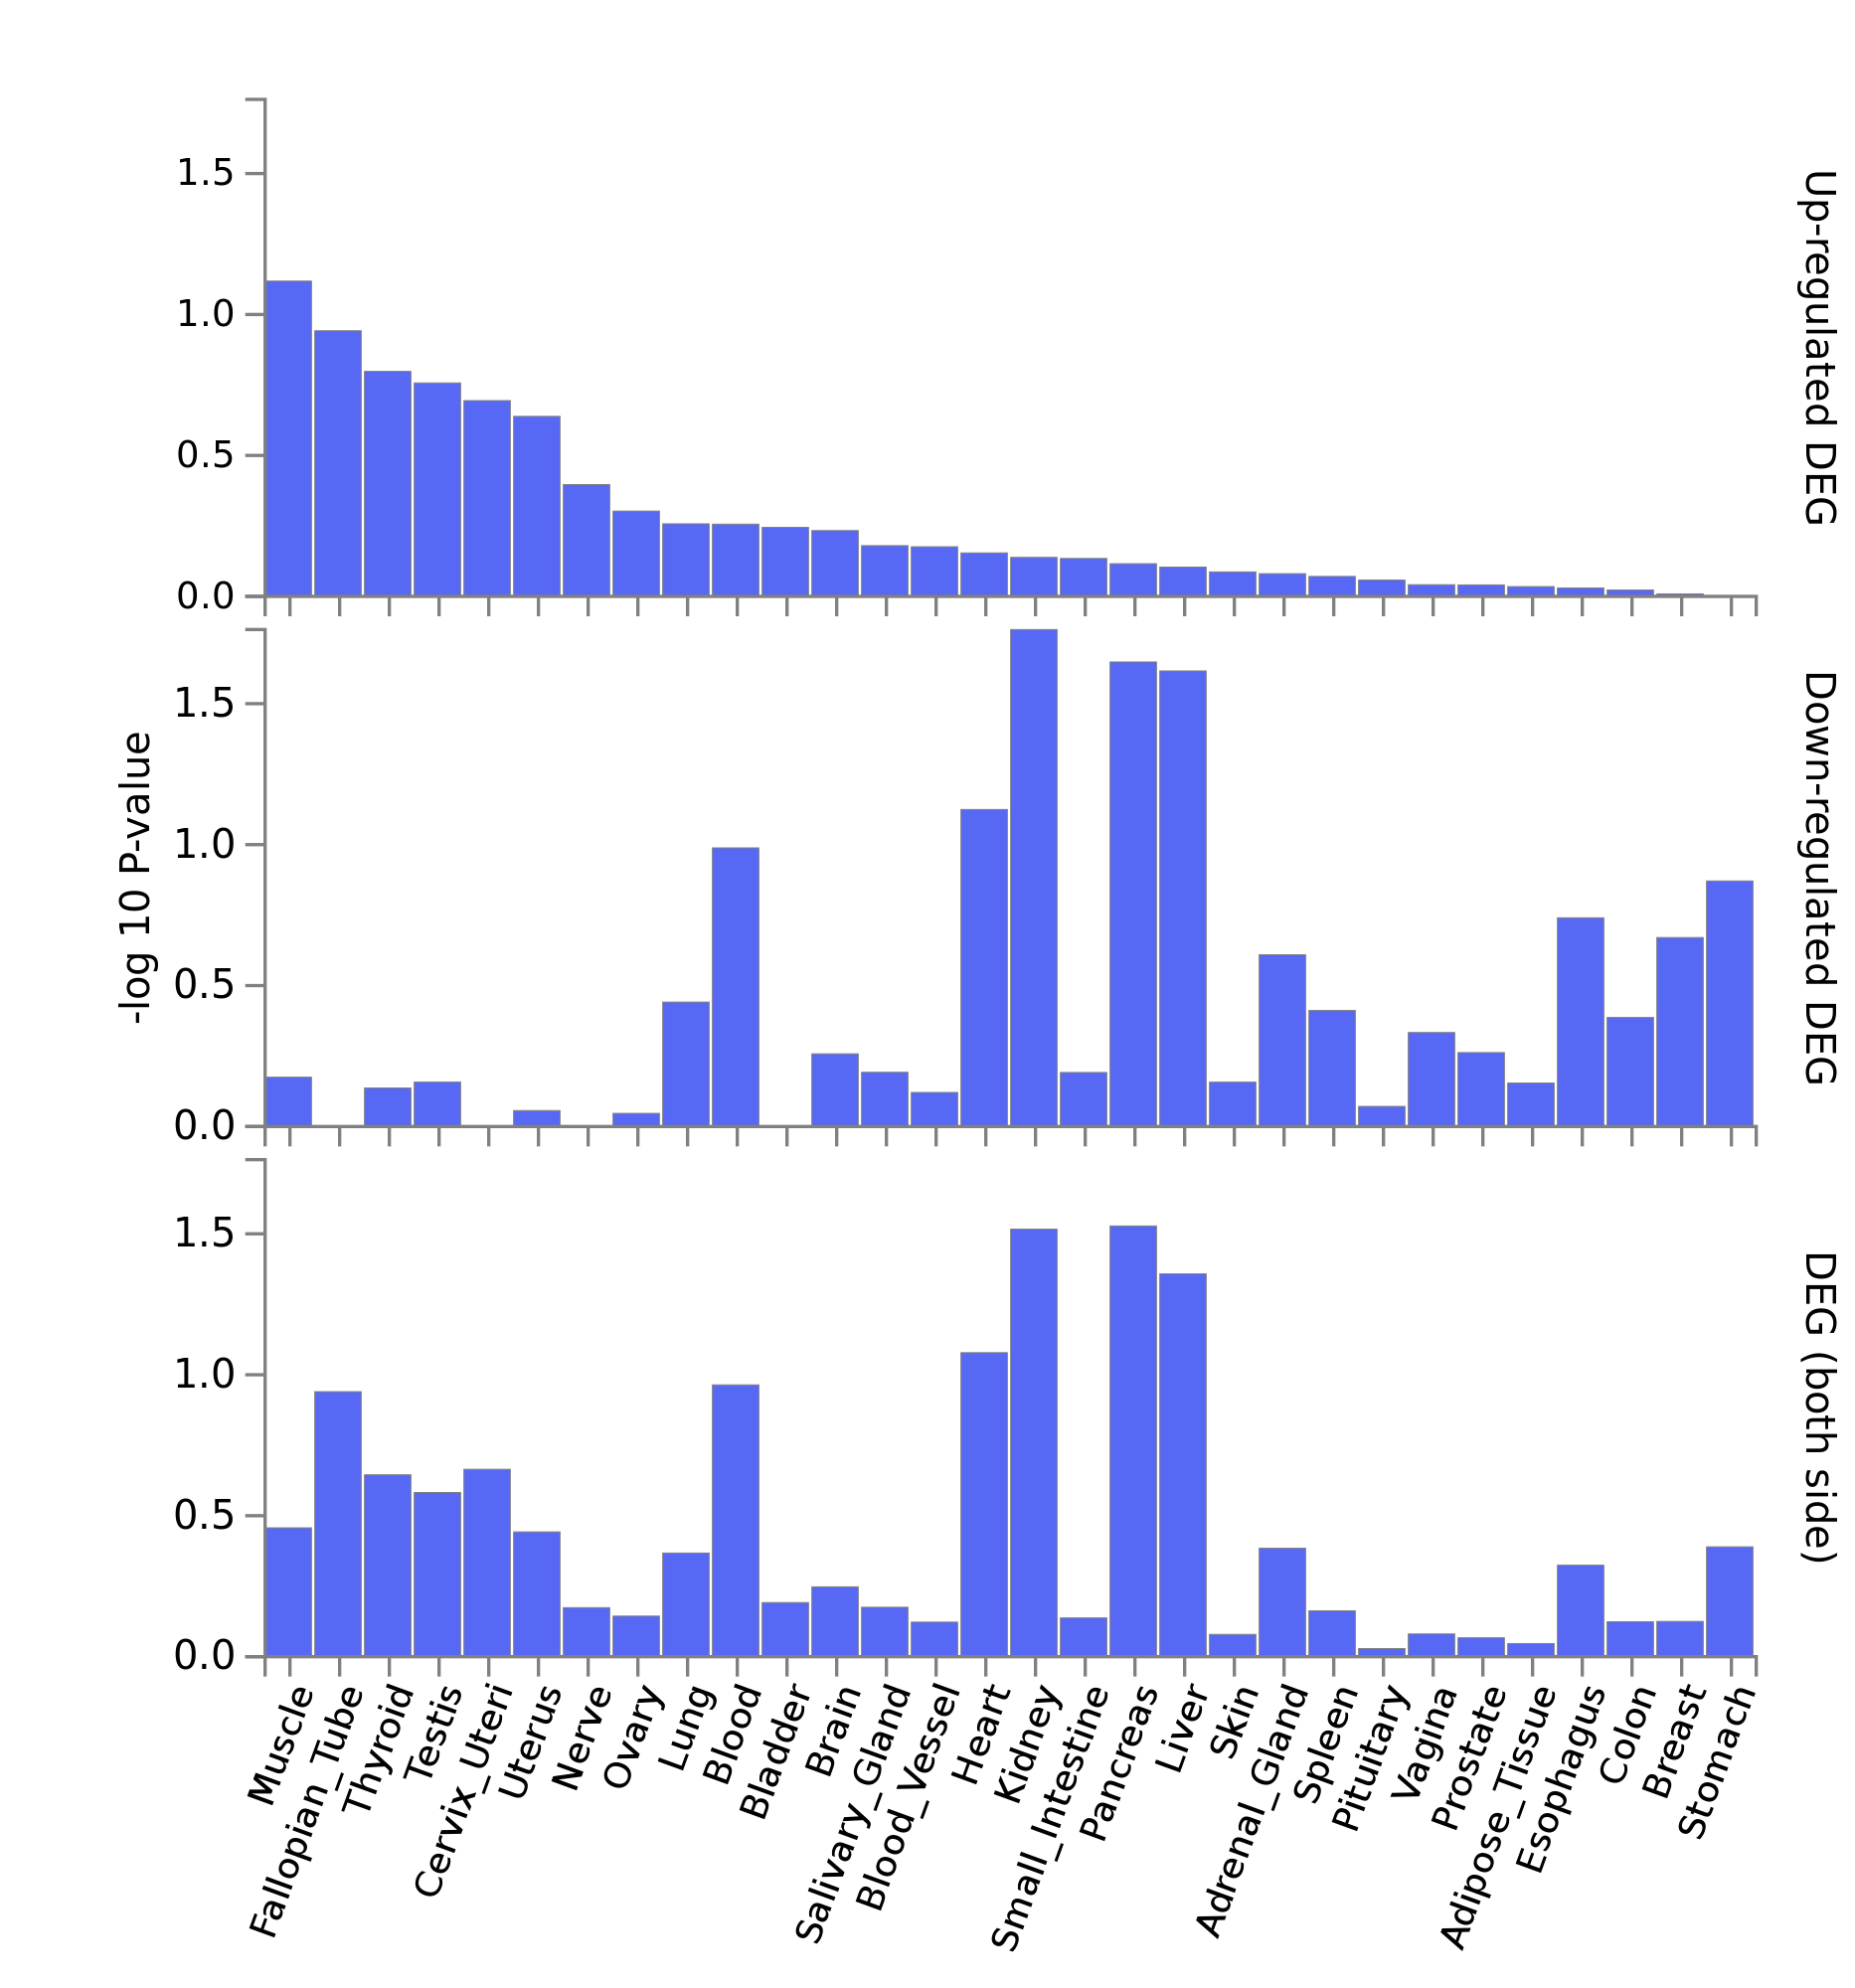
\includegraphics[width=\textwidth]{images/FUMA_plots/ctg_upregulated30tissues_46_genes.png}
%     \caption{GTEx upregulation in significant genes in Intelligence\textsubscript{Replication} sample. $-log_10(0.05)=1.301$}
%     \label{fig:GTEX FUMA CTG}
% \end{figure}
% \paragraph{toppfun}
% CC
% ID 	Name 	Source 	pValue 	FDR BH 	FDR BY 	Bonferroni 	Genes from Input 	Genes in Annotation 
% GO:0032584 	growth cone membrane 		1.416E-4 	3.838E-2 	
% 2.373E-1
% 	3.838E-2 	2 	8% latex table generated in R 3.6.3 by xtable 1.8-4 package
% % Tue Sep 15 11:43:35 2020

% \paragraph{topp fun PSP background}
% Nil MF,BP,CC Nothing at all


\subsection{Education\textsubscript{Replication} Gene Ontology analysis}
Okbay et al.\cite{okbay2016genome} report using DEPICT\cite{pers2015biological} to investigate pathway enrichment in genes near significant SNPs. 283 gene sets were determined to be significant and clustered into five groups: ``neural progenitor cells, migration of new neurons to cortex, projection of axons to target, sprouting of dendrites and spines, and neuronal signalling and synaptic plasticity throughout the lifespan''\cite{okbay2016genome}\todo{check quote}. An association with genetic variants identified and  genes involved in intellectual disability was also reported. The Education\textsubscript{Replication} sample differs from that reported by Okbay et al. \cite{okbay2016genome} as results obtained from UK Biobank and the individuals from 23andme are excluded (see section~\ref{sec:Edcuation replication gwgas}).



 \subsection{PANTHER Gene Ontology analysis Education\textsubscript{Replication}}
 
 The significant genes were again formatted to maximise the number identified in PANTHER\footnote{HGNC id from Symbols from NCBI from MAGMA\url{source('~/RProjects/paper_xls_output/R/chapter_2/translate_sig_genes/ea2_NCBI_translate2.R')}}
 Using the default background and FDR to correct for multiple comparisons, nineteen biological process terms were found to be enriched. No molecular function or cellular component terms were enriched. No enrichment was seen in PANTHER protein class, pathways (including Reactome pathways) or for any of the SLIM ontologies. 
 
%  Pathways nil
%  SLIM BP,MF,CC nil
 
%  Protein class nil
 
%  Reactome pathways nil
 
  %   \url{source('~/RProjects/paper_xls_output/R/chapter_2/translate_sig_genes/ea2_NCBI_translate2.R')}
     
   %  HGNC id from Symbols from NCBI from MAGMA
     
%      Fails to recognise 18839 but recognised STH which is HGNC18839. With HGNC symbols. 2 dual mapped MST1 to MST1	2 	HUMAN|HGNC=11408|UniProtKB=Q13043,
% HUMAN|HGNC=7380|UniProtKB=P26927
% but has the correct entrez 4485 (MAGMA output) P26927 MST1 (hepatocyte growth factor) other is Q13043 stk4 
%  99 entrez genes. Using approved HGNC symbols from NCBI get 1000 as maps MST1 to STK4
 
%  Using HGNC symbols as input does not recognise 11408 (comes from same output) which is STH which it always has difficulty with inputing STH is recognised and finds HGNC18839 don't know how to get round this
 The PANTHER enrichment displays the hierarchy of the ontology terms; although the FDR values are lower than ToppGene the very specific term related to neurogenesis, "positive regulation of collateral sprouting" (FDR p 0.041) is prominent in comparison to the same data ordered by FDR shown in table~\ref{tab:GO.biological.process.complete Panther Gene Ontology Enrichment significant genes in Education Replication}. There is also a considerable difference in actual enrichment values, including the raw $p$ value calculated in ToppGene and PANTHER. Widely variant scores are noted in Rhee (2008) \cite{rhee2008use} and see Khatri et al. for a detailed discussion \cite{khatri2005ontological}.
 \footnote{Douglas: I have included this as a screenshot. Parsing the xml and getting it into latex took longer than I thou
 ght so I went straight to screenshot as a last resort could do the indentation by hand. Thought worth showing (as DEPICT, MAGMA etc as far as I can see ignore heirarchy) but interested in what you thought. The standard table output for PANTHER doesn't have the hierarchy. I thought the differences in approach to the GO DAG were worth discussing  - as part of pointing out limitations to how enrichment has been approached in genomics. }
 
F No significant enrichment was seen using PANTHER for molecular function or cellular function. Biological function was enriched for 19 terms using FDR to correct for multiple comparisons. The most enriched term is "nervous system development" (GO:0007399), FDR q = 0.006, but the term is the largest and most general with 2430 members in the annotation. (table~\ref{tab:GO biological process complete Education Replication FDRover represenation only}). "Positive regulation of collateral sprouting",GO:0048672, is just below nominal significance after correction for multiple comparisons using FDR but is a very specific term with over 52 times fold enrichment and 3 of the 12 genes annotated to this term are significant genes in GWGAS. This balance between significance and specificity is an issue to some extent for all GO pathway analyses (see fig~\ref{tab:GO biological process complete Education Replication FDR} and table~\ref{tab:GO biological process complete Education Replication FDRover represenation only}). No PANTHER SLIM ontology term showed significant enrichment. 

 \begin{figure}
     \centering
     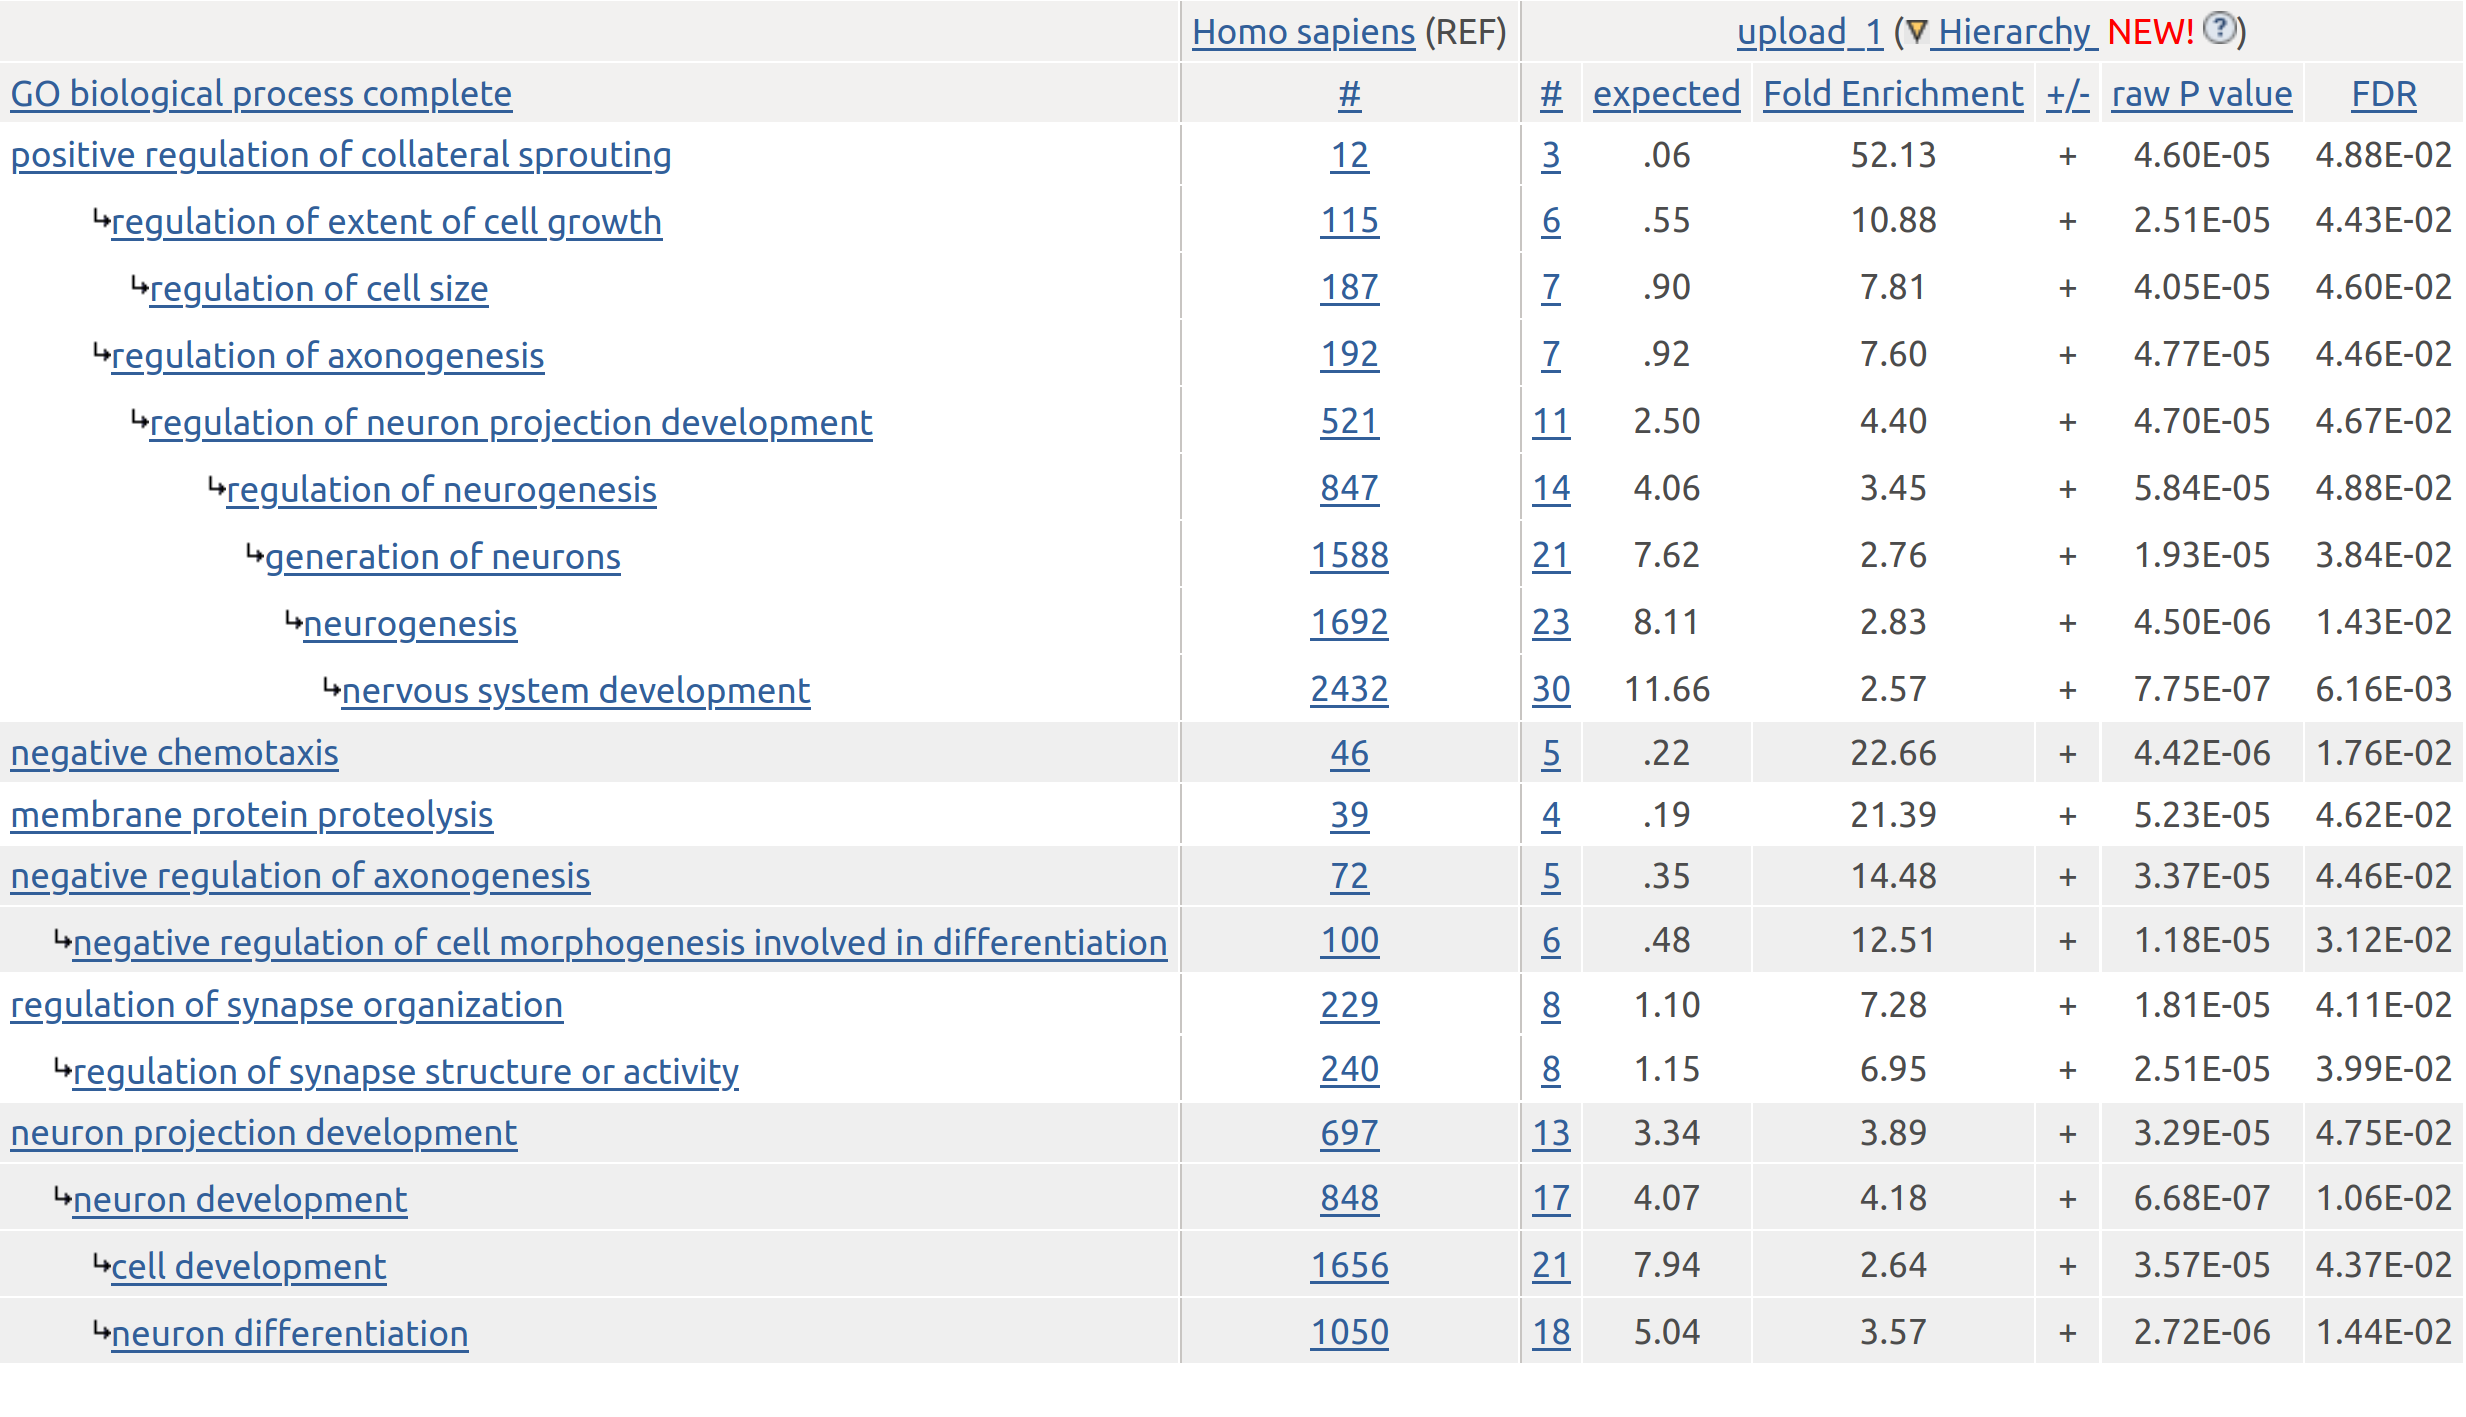
\includegraphics[width=\textwidth]{images/chapter2/large_screenshots/edu_replication_large_bp_panther.png}
     \caption[GO enrichment PANTHER Biological Process Education\textsubscript{Replication}]{GO enrichment of genome wide significant genes at GWGAS in the Education\textsubscript{Replication} cohort. Enrichment calculated
     using PANTHER with Fisher's exact test for the over representation test and using the False Discovery Rate correction for multiple comparisons. The term with the lowest FDR is GO:0007399 nervous system development (FDR 0.006). The figure shows the hierarchy of Gene Ontology terms, the most general terms are the most indented, the deepest terms in the directed acyclic graph are the most indented. Child terms are indented underneath their adult terms. Terms with identical levels of indentation are at identical layers in the hierarchy. Text output in \url{/home/grant/RProjects/paper_xls_output/data/PANTHER_txt_output/checked_for_thesis/ea2/BP_all.txt}}%previous image images/screenshots/EA2_BP_Panther_all_genes_FDR.png}
     
     \label{tab:GO biological process complete Education Replication FDR}
 \end{figure}
 % latex table generated in R 3.6.3 by xtable 1.8-4 package
% Tue Sep  1 11:07:38 2020


\begin{figure}
    \centering
    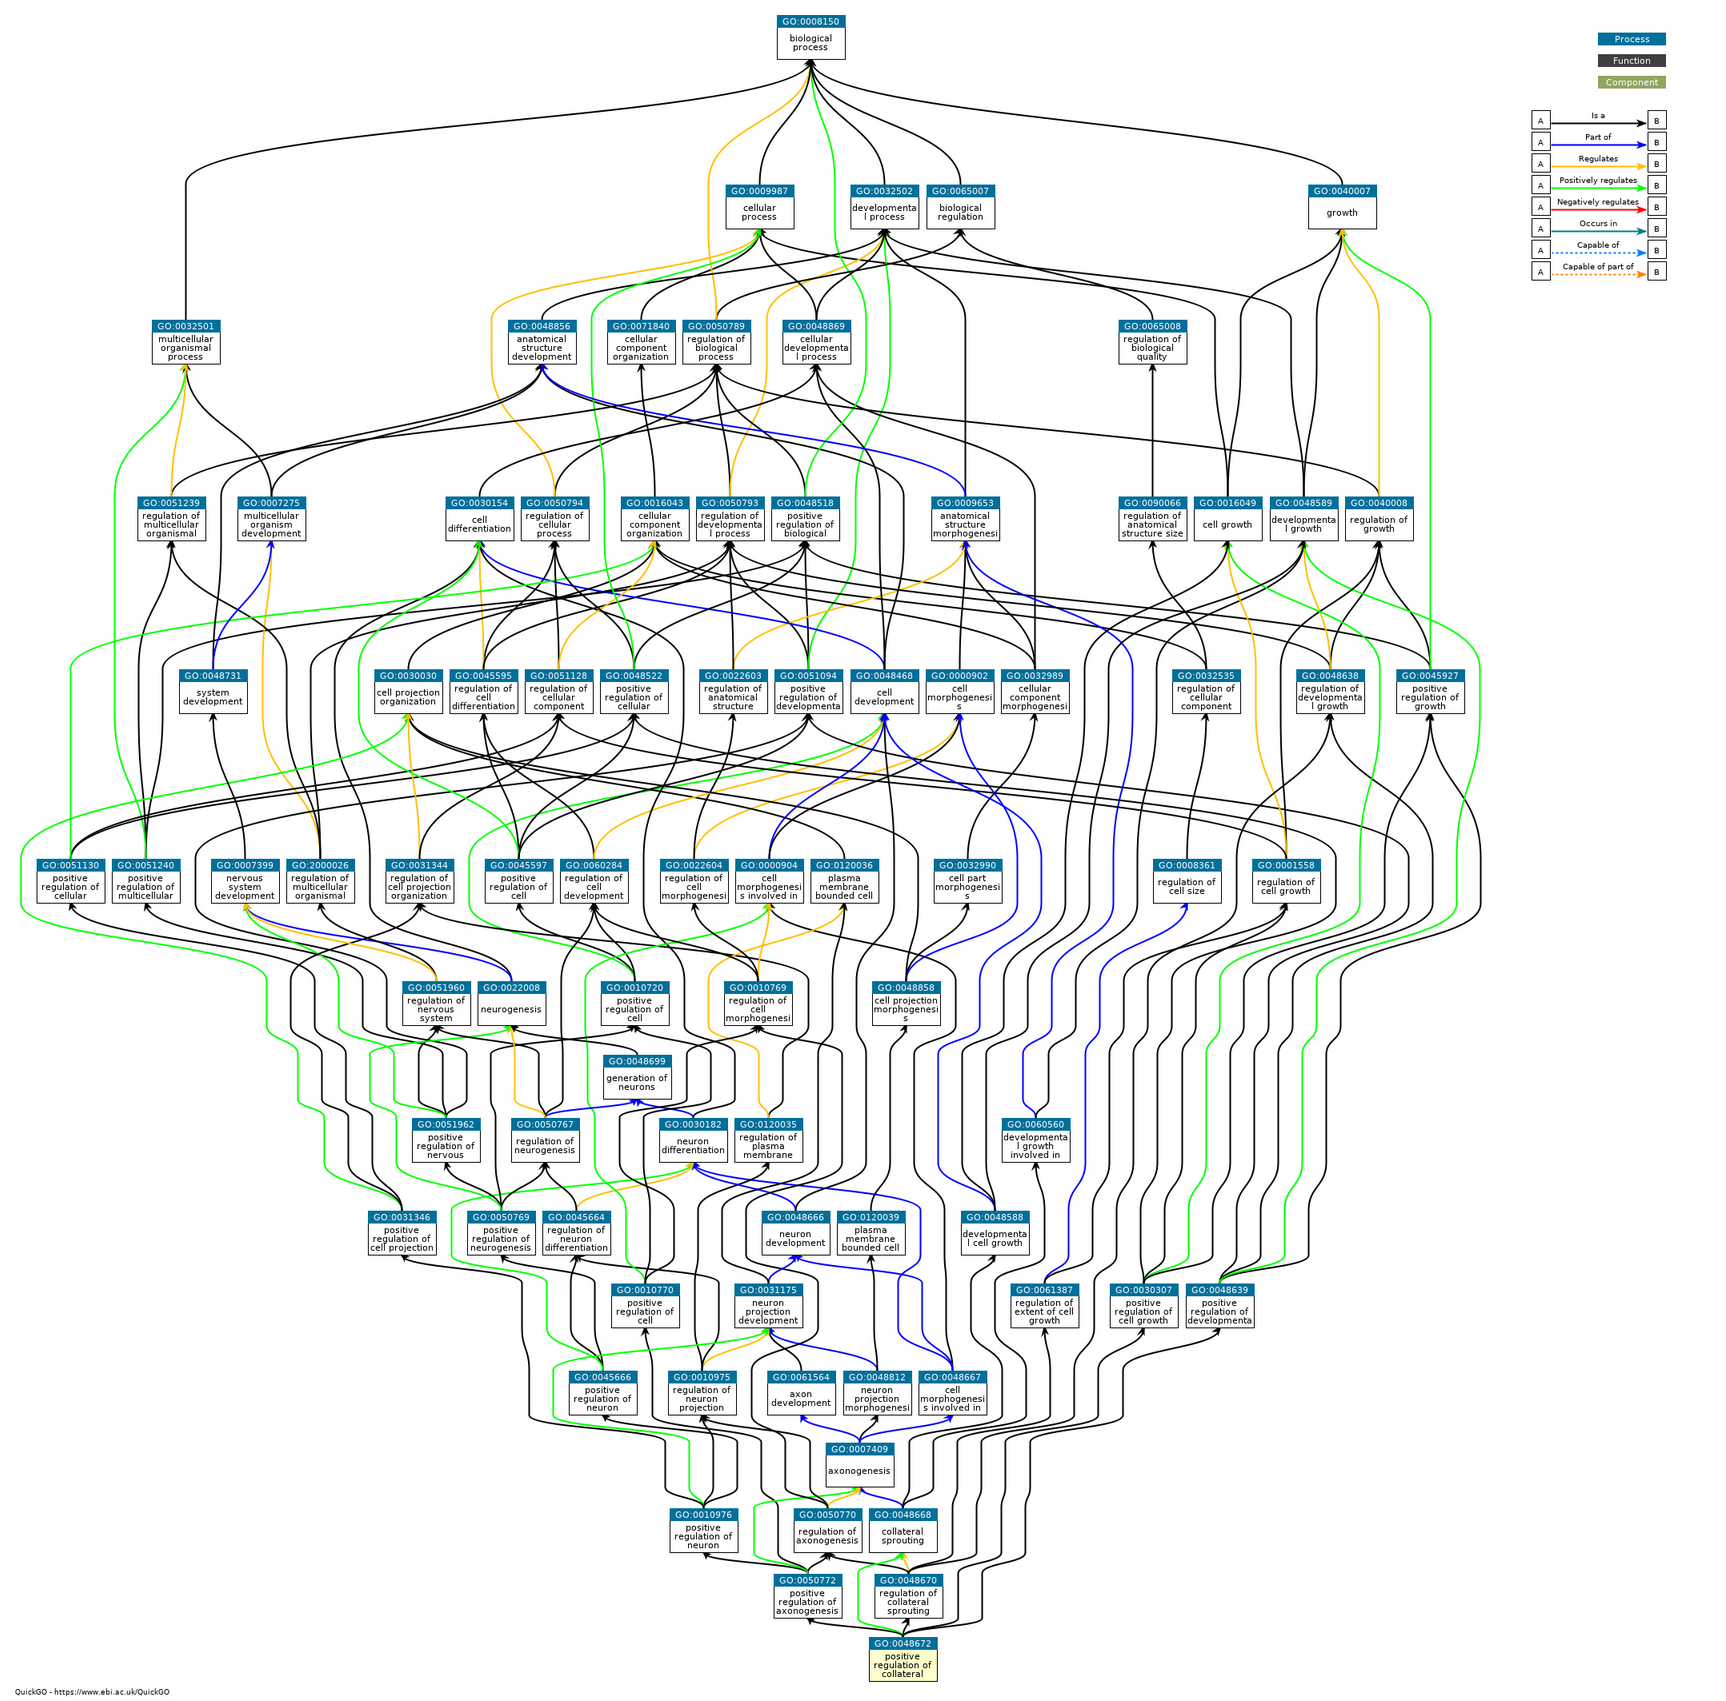
\includegraphics[width=\textwidth]{images/screenshots/quick_go_collateral.png}
    \caption{Gene Ontology Hierarchy of Biological Process term Collateral Sprouting from Quick GO. Although FDR q level is modest, in Education\textsubscript{Replication}, the fold change for the term is marked. Image source Quick GO. The term related to other terms such as growth cone development and neuron projection development (GO:0031175) found in both Education samples and in the paper by \cite{okbay2016genome}.How to prioritise such specific terms over general terms is an issue faced by GO enrichment methods.}
    \label{fig:the DAG of Collateral sprouting}
\end{figure}

% \begin{table}[ht]
% \resizebox{\textwidth}{!}{%
% \centering

% \begin{tabular}{llrrrrrr}
%   \hline
% GO & description & Ref & Test & E & Fold & P & FDR \\ 
%   \hline
% GO:0048672 & positive regulation of collateral sprouting  & 12 & 3 & 0.1 & 52.13 & $4.60 \times 10^{-5}$ & 0.049 \\ 
%   GO:0050919 & negative chemotaxis  & 46 & 5 & 0.2 & 22.66 & $4.42 \times 10^{-6}$ & 0.014 \\ 
%   GO:0033619 & membrane protein proteolysis  & 39 & 4 & 0.2 & 21.39 & $5.23 \times 10^{-5}$ & 0.046 \\ 
%   GO:0050771 & negative regulation of axonogenesis  & 72 & 5 & 0.3 & 14.48 & $3.37 \times 10^{-5}$ & 0.045 \\ 
%   GO:0010771 & negative regulation of cell morphogenesis involved in differentiation  & 100 & 6 & 0.5 & 12.51 & $1.18 \times 10^{-5}$ & 0.031 \\ 
%   GO:0061387 & regulation of extent of cell growth  & 115 & 6 & 0.6 & 10.88 & $2.51 \times 10^{-5}$ & 0.044 \\ 
%   GO:0008361 & regulation of cell size  & 187 & 7 & 0.9 & 7.81 & $4.05 \times 10^{-5}$ & 0.046 \\ 
%   GO:0050770 & regulation of axonogenesis  & 192 & 7 & 0.9 & 7.60 & $4.77 \times 10^{-5}$ & 0.045 \\ 
%   GO:0050807 & regulation of synapse organization  & 229 & 8 & 1.1 & 7.28 & $1.81 \times 10^{-5}$ & 0.041 \\ 
%   GO:0050803 & regulation of synapse structure or activity  & 240 & 8 & 1.1 & 6.95 & $2.51 \times 10^{-5}$ & 0.040 \\ 
%   GO:0010975 & regulation of neuron projection development  & 521 & 11 & 2.5 & 4.40 & $4.70 \times 10^{-5}$ & 0.047 \\ 
%   GO:0048666 & neuron development  & 848 & 17 & 4.1 & 4.18 & $6.68 \times 10^{-7}$ & 0.011 \\ 
%   GO:0031175 & neuron projection development  & 697 & 13 & 3.3 & 3.89 & $3.29 \times 10^{-5}$ & 0.048 \\ 
%   GO:0030182 & neuron differentiation  & 1046 & 18 & 5.0 & 3.59 & $2.58 \times 10^{-6}$ & 0.014 \\ 
%   GO:0050767 & regulation of neurogenesis  & 847 & 14 & 4.1 & 3.45 & $5.84 \times 10^{-5}$ & 0.049 \\ 
%   GO:0022008 & neurogenesis  & 1690 & 23 & 8.1 & 2.84 & $4.42 \times 10^{-6}$ & 0.018 \\ 
%   GO:0048699 & generation of neurons  & 1585 & 21 & 7.6 & 2.76 & $1.88 \times 10^{-5}$ & 0.037 \\ 
%   GO:0048468 & cell development  & 1654 & 21 & 7.9 & 2.65 & $3.51 \times 10^{-5}$ & 0.043 \\ 
%   GO:0007399 & nervous system development  & 2430 & 30 & 11.7 & 2.57 & $7.62 \times 10^{-7}$ & 0.006 \\ 
%   \hline
% \end{tabular}}
% \caption{GO biological process complete Education Replication FDRover represenation only  Ref reference set, test:number of genes being tested present in ontology termE expected number of genes being tested present in ontology term, Fold= Fold change P = raw p value, FDR = false discovery rate} 
% \label{tab:GO biological process complete Education Replication FDRover represenation only}
% \end{table}
 
%  % latex table generated in R 3.6.3 by xtable 1.8-4 package
% % Sat Aug 29 13:31:48 2020
% \begin{table}[ht]
% \centering
% \begin{tabular}{llrrrlrr}
%   \hline
% GO & description & Ref & Test & E & OU & Fold & P Bnf \\ 
%   \hline
% GO:0050919 & negative chemotaxis  & 46 & 5 & 0.2  & + & 22.66 & 0.040 \\ 
%   GO:0048666 & neuron development  & 848 & 17 & 4.1 & + & 4.18 & 0.006 \\ 
%   GO:0030182 & neuron differentiation  & 1046 & 18 & 5.0 & + & 3.59 & 0.023 \\ 
%   GO:0022008 & neurogenesis  & 1690 & 23 & 8.1 & + & 2.84 & 0.040 \\ 
%   GO:0007399 & nervous system development  & 2430 & 30 & 11.7 & + & 2.57 & 0.007 \\ 
%   UNCLASSIFIED & Unclassified  & 2924 & 7 & 14.0 & - & 0.50 & 0.000 \\ 
%   \hline
% \end{tabular}
% \caption{GO biological process complete Education Replication Bonferroni} 
% \label{tab:GO biological process complete Education Replication Bonferroni}
% \end{table}

 % latex table generated in R 3.6.3 by xtable 1.8-4 package
% Sat Aug 29 14:04:17 2020
\begin{table}[ht]
\centering
\begin{tabular}{llrrrrrr}
  \hline
GO & description & Ref & Test & E & Fold & P & FDR \\ 
  \hline
GO:0048672 & positive regulation of collateral sprouting  & 12 & 3 & 0.1 & 52.13 & $4.600 \times 10^{-5}$ & 0.049 \\ 
  GO:0050919 & negative chemotaxis  & 46 & 5 & 0.2 & 22.66 & $4.420 \times 10^{-6}$ & 0.014 \\ 
  GO:0033619 & membrane protein proteolysis  & 39 & 4 & 0.2 & 21.39 & $5.230 \times 10^{-5}$ & 0.046 \\ 
  GO:0050771 & negative regulation of axonogenesis  & 72 & 5 & 0.3 & 14.48 & $3.370 \times 10^{-5}$ & 0.045 \\ 
  GO:0010771 & \makecell{negative regulation of cell morphogenesis\\ involved in differentiation}  & 100 & 6 & 0.5 & 12.51 & $1.180 \times 10^{-5}$ & 0.031 \\ 
  GO:0061387 & regulation of extent of cell growth  & 115 & 6 & 0.6 & 10.88 & $2.510 \times 10^{-5}$ & 0.044 \\ 
  GO:0008361 & regulation of cell size  & 187 & 7 & 0.9 & 7.81 & $4.050 \times 10^{-5}$ & 0.046 \\ 
  GO:0050770 & regulation of axonogenesis  & 192 & 7 & 0.9 & 7.60 & $4.770 \times 10^{-5}$ & 0.045 \\ 
  GO:0050807 & regulation of synapse organization  & 229 & 8 & 1.1 & 7.28 & $1.810 \times 10^{-5}$ & 0.041 \\ 
  GO:0050803 & regulation of synapse structure or activity  & 240 & 8 & 1.1 & 6.95 & $2.510 \times 10^{-5}$ & 0.040 \\ 
  GO:0010975 & regulation of neuron projection development  & 521 & 11 & 2.5 & 4.40 & $4.700 \times 10^{-5}$ & 0.047 \\ 
  GO:0048666 & neuron development  & 848 & 17 & 4.1 & 4.18 & $6.680 \times 10^{-7}$ & 0.011 \\ 
  GO:0031175 & neuron projection development  & 697 & 13 & 3.3 & 3.89 & $3.290 \times 10^{-5}$ & 0.048 \\ 
  GO:0030182 & neuron differentiation  & 1046 & 18 & 5.0 & 3.59 & $2.580 \times 10^{-6}$ & 0.014 \\ 
  GO:0050767 & regulation of neurogenesis  & 847 & 14 & 4.1 & 3.45 & $5.840 \times 10^{-5}$ & 0.049 \\ 
  GO:0022008 & neurogenesis  & 1690 & 23 & 8.1 & 2.84 & $4.420 \times 10^{-6}$ & 0.018 \\ 
  GO:0048699 & generation of neurons  & 1585 & 21 & 7.6 & 2.76 & $1.880 \times 10^{-5}$ & 0.037 \\ 
  GO:0048468 & cell development  & 1654 & 21 & 7.9 & 2.65 & $3.510 \times 10^{-5}$ & 0.043 \\ 
  GO:0007399 & nervous system development  & 2430 & 30 & 11.7 & 2.57 & $7.620 \times 10^{-7}$ & 0.006 \\ 
   \hline
\end{tabular}
\caption{GO biological process complete PANTHER Education\textsubscript{Replication} FDR over representation only. Ref reference set, test:number of genes being tested present in ontology term, E expected number of genes being tested present in ontology term, Fold= Fold change, P = raw p value, FDR = false discovery rate \url{source('~/RProjects/paper_xls_output/R/chapter_2/make_PANTHER_tables/make_Panther_table_GO_col_nounderFDR.R')}} 
\label{tab:GO biological process complete Education Replication FDRover represenation only}
\end{table}


Using FUMA GTex enrichment I found no statistically significant differential enrichment for the genes in the central nervous system (figure~\ref{fig:FUMA gtex deg samples multiple} and fig~\ref{fig:deg_upref_sample_gtex_gener})



% \begin{figure}
%     \centering
%     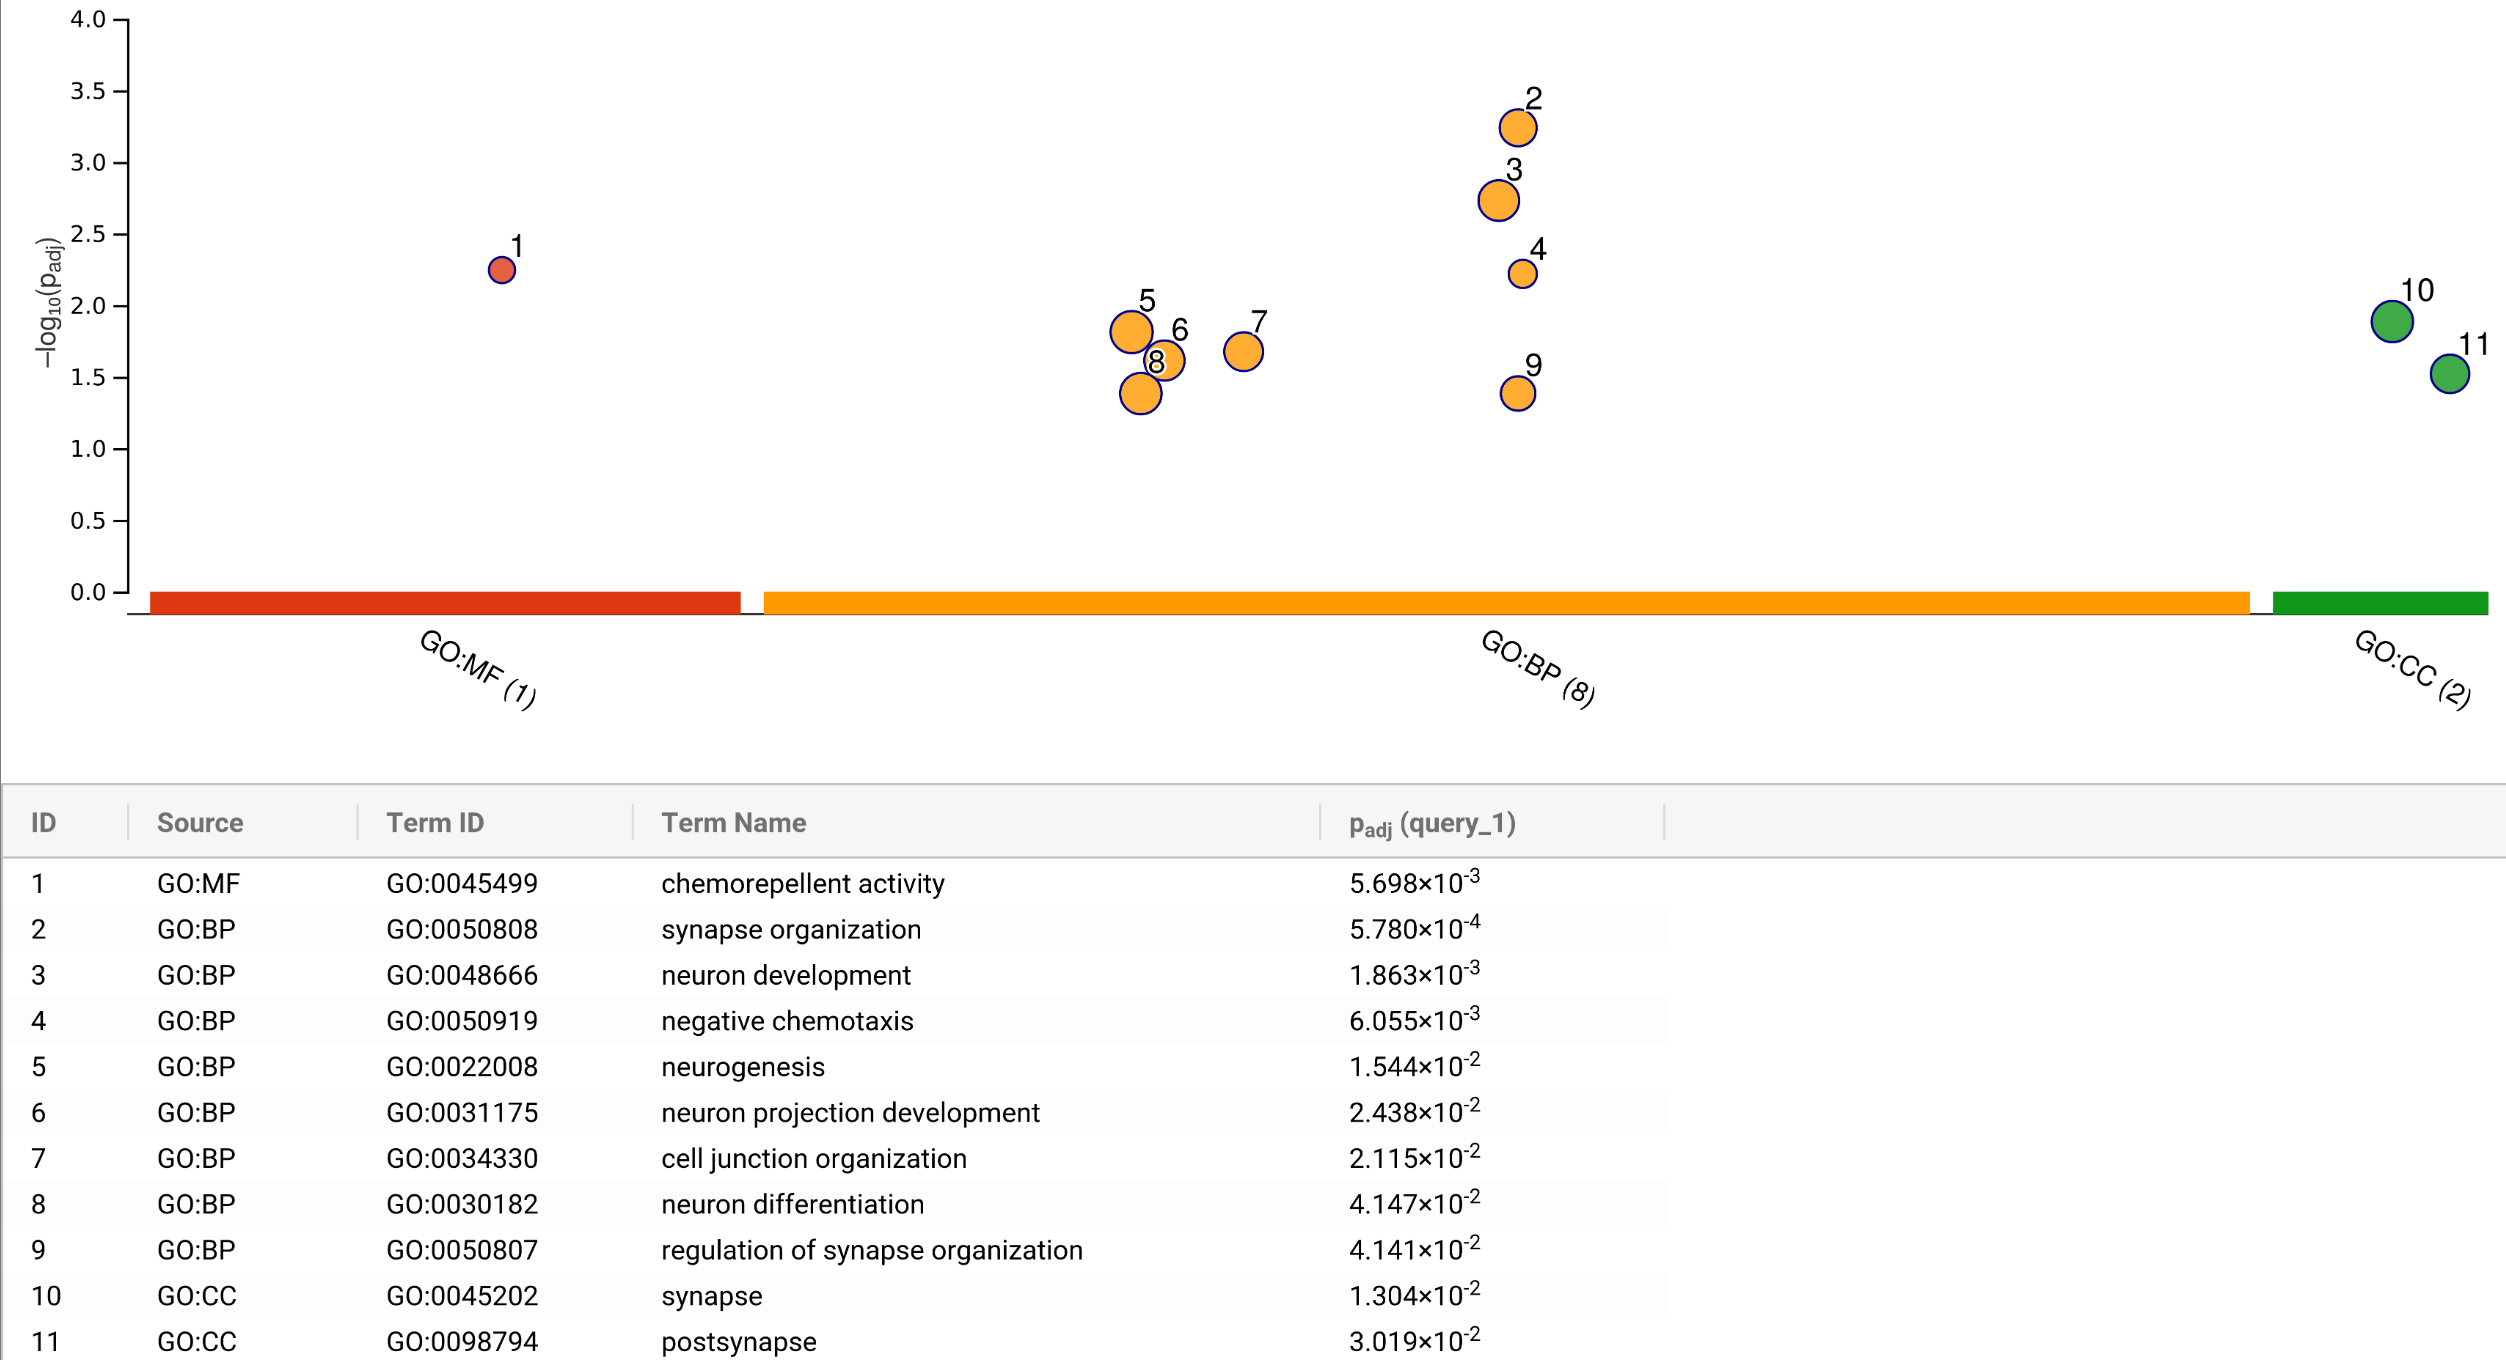
\includegraphics[width=\textwidth]{images/gprofiler/gprofiler_ea2_clip.png}
%     \caption{GO enrichment for significant genes using gProfiler multiple testing control SGS. Educational\textsubscript{Replication} sample}
    
%     \label{fig:gprofiler_ea2}
% \end{figure}

% \begin{figure}
%     \centering
%     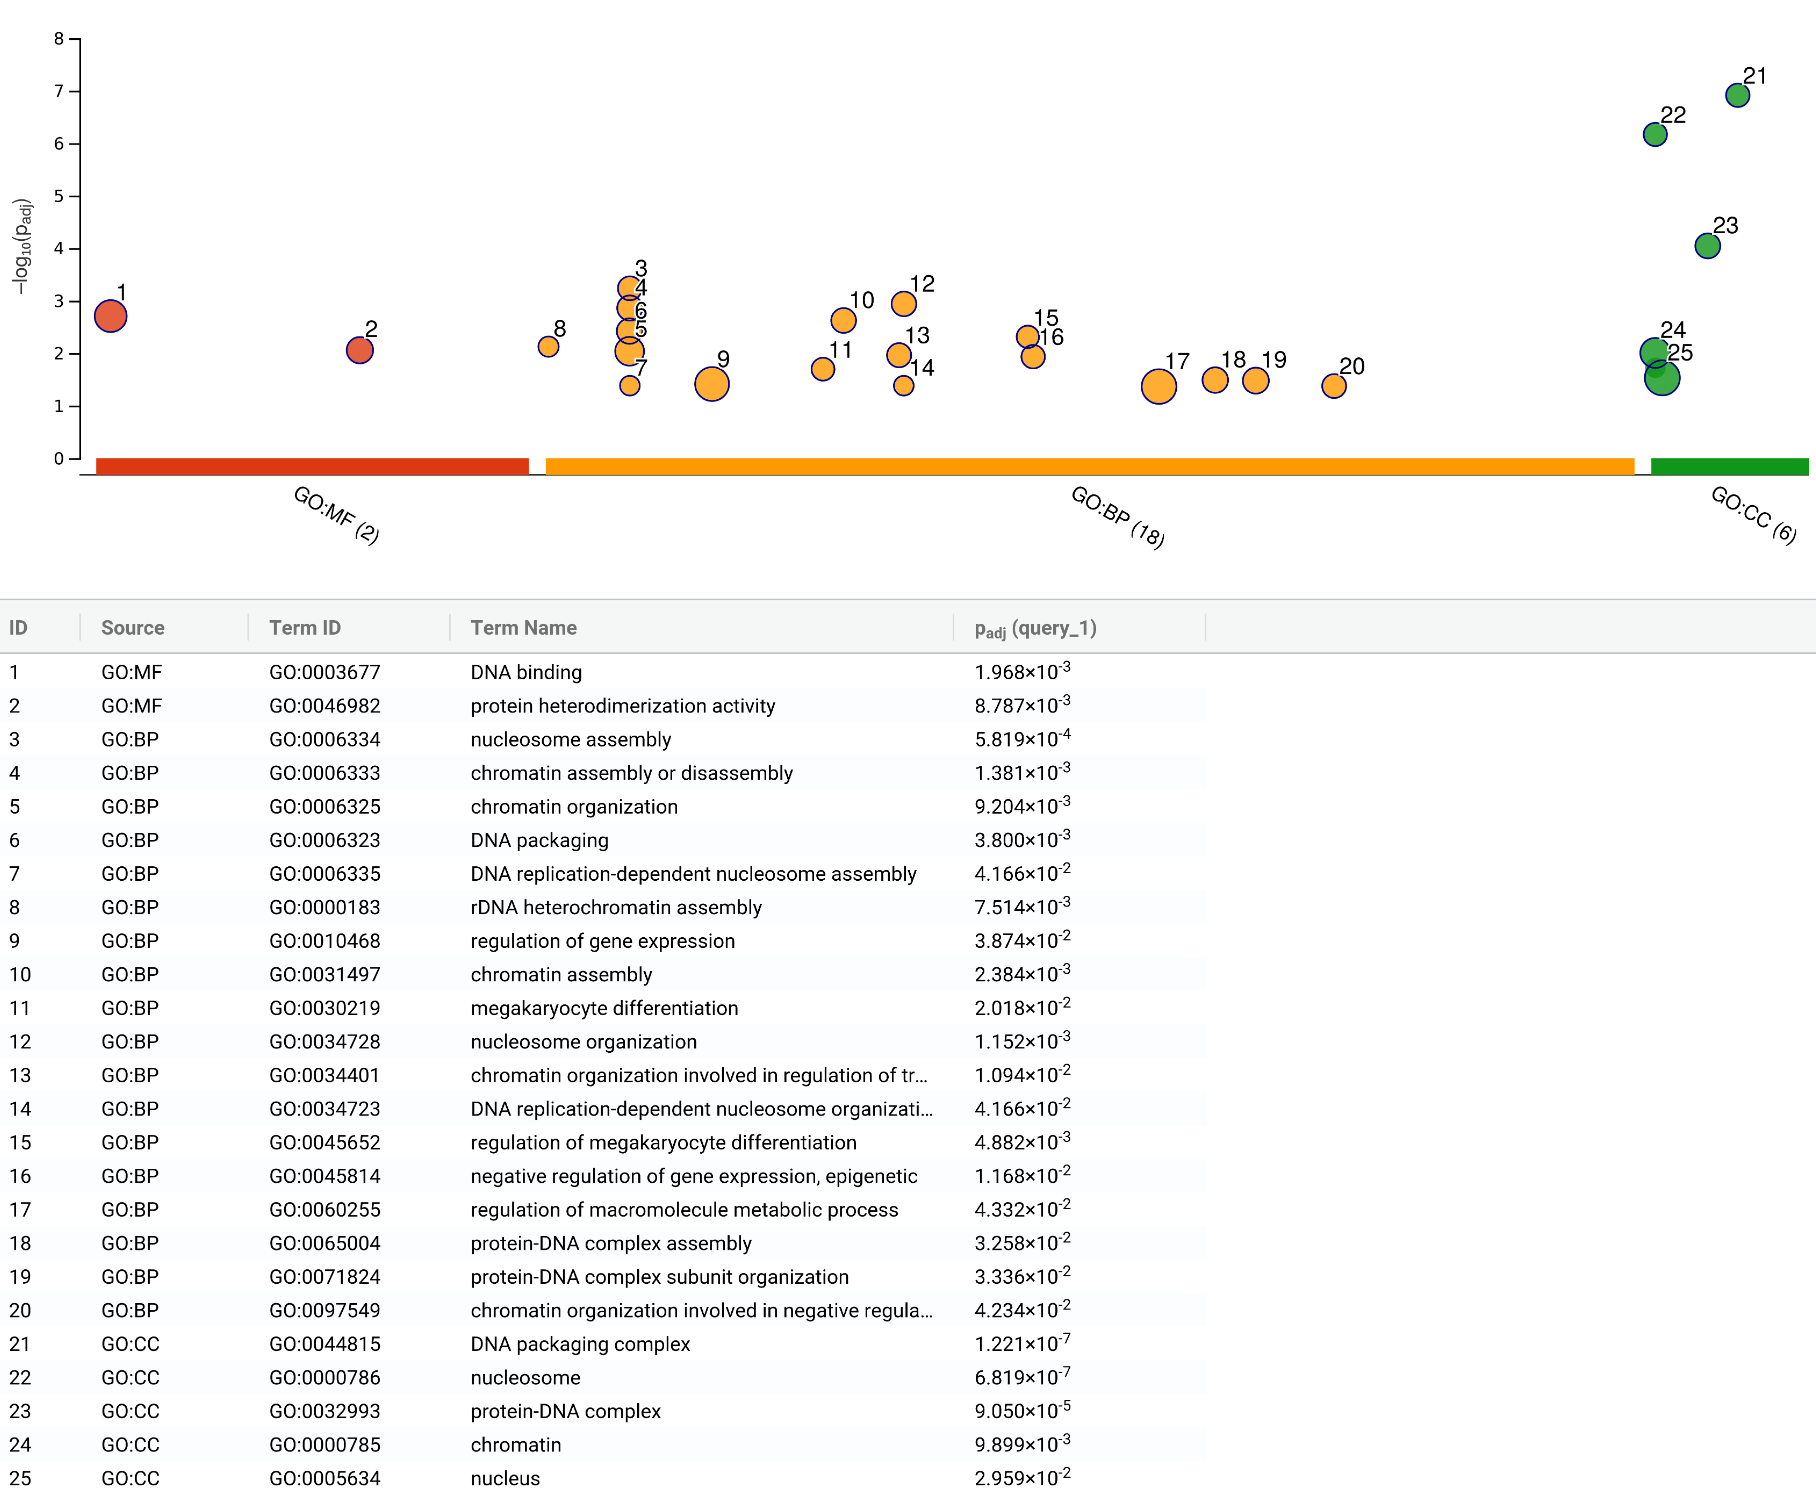
\includegraphics[width=\textwidth]{images/gprofiler/gprofiler_ukbbint_clip.png}
%     \caption{GO enrichment for significant genes using gProfiler multiple testing control SGS. Intelligence\textsubscript{Discovery} sample}
%     \label{fig:gprofiler_ukbbint}
% \end{figure}

% \begin{figure}
%     \centering
%     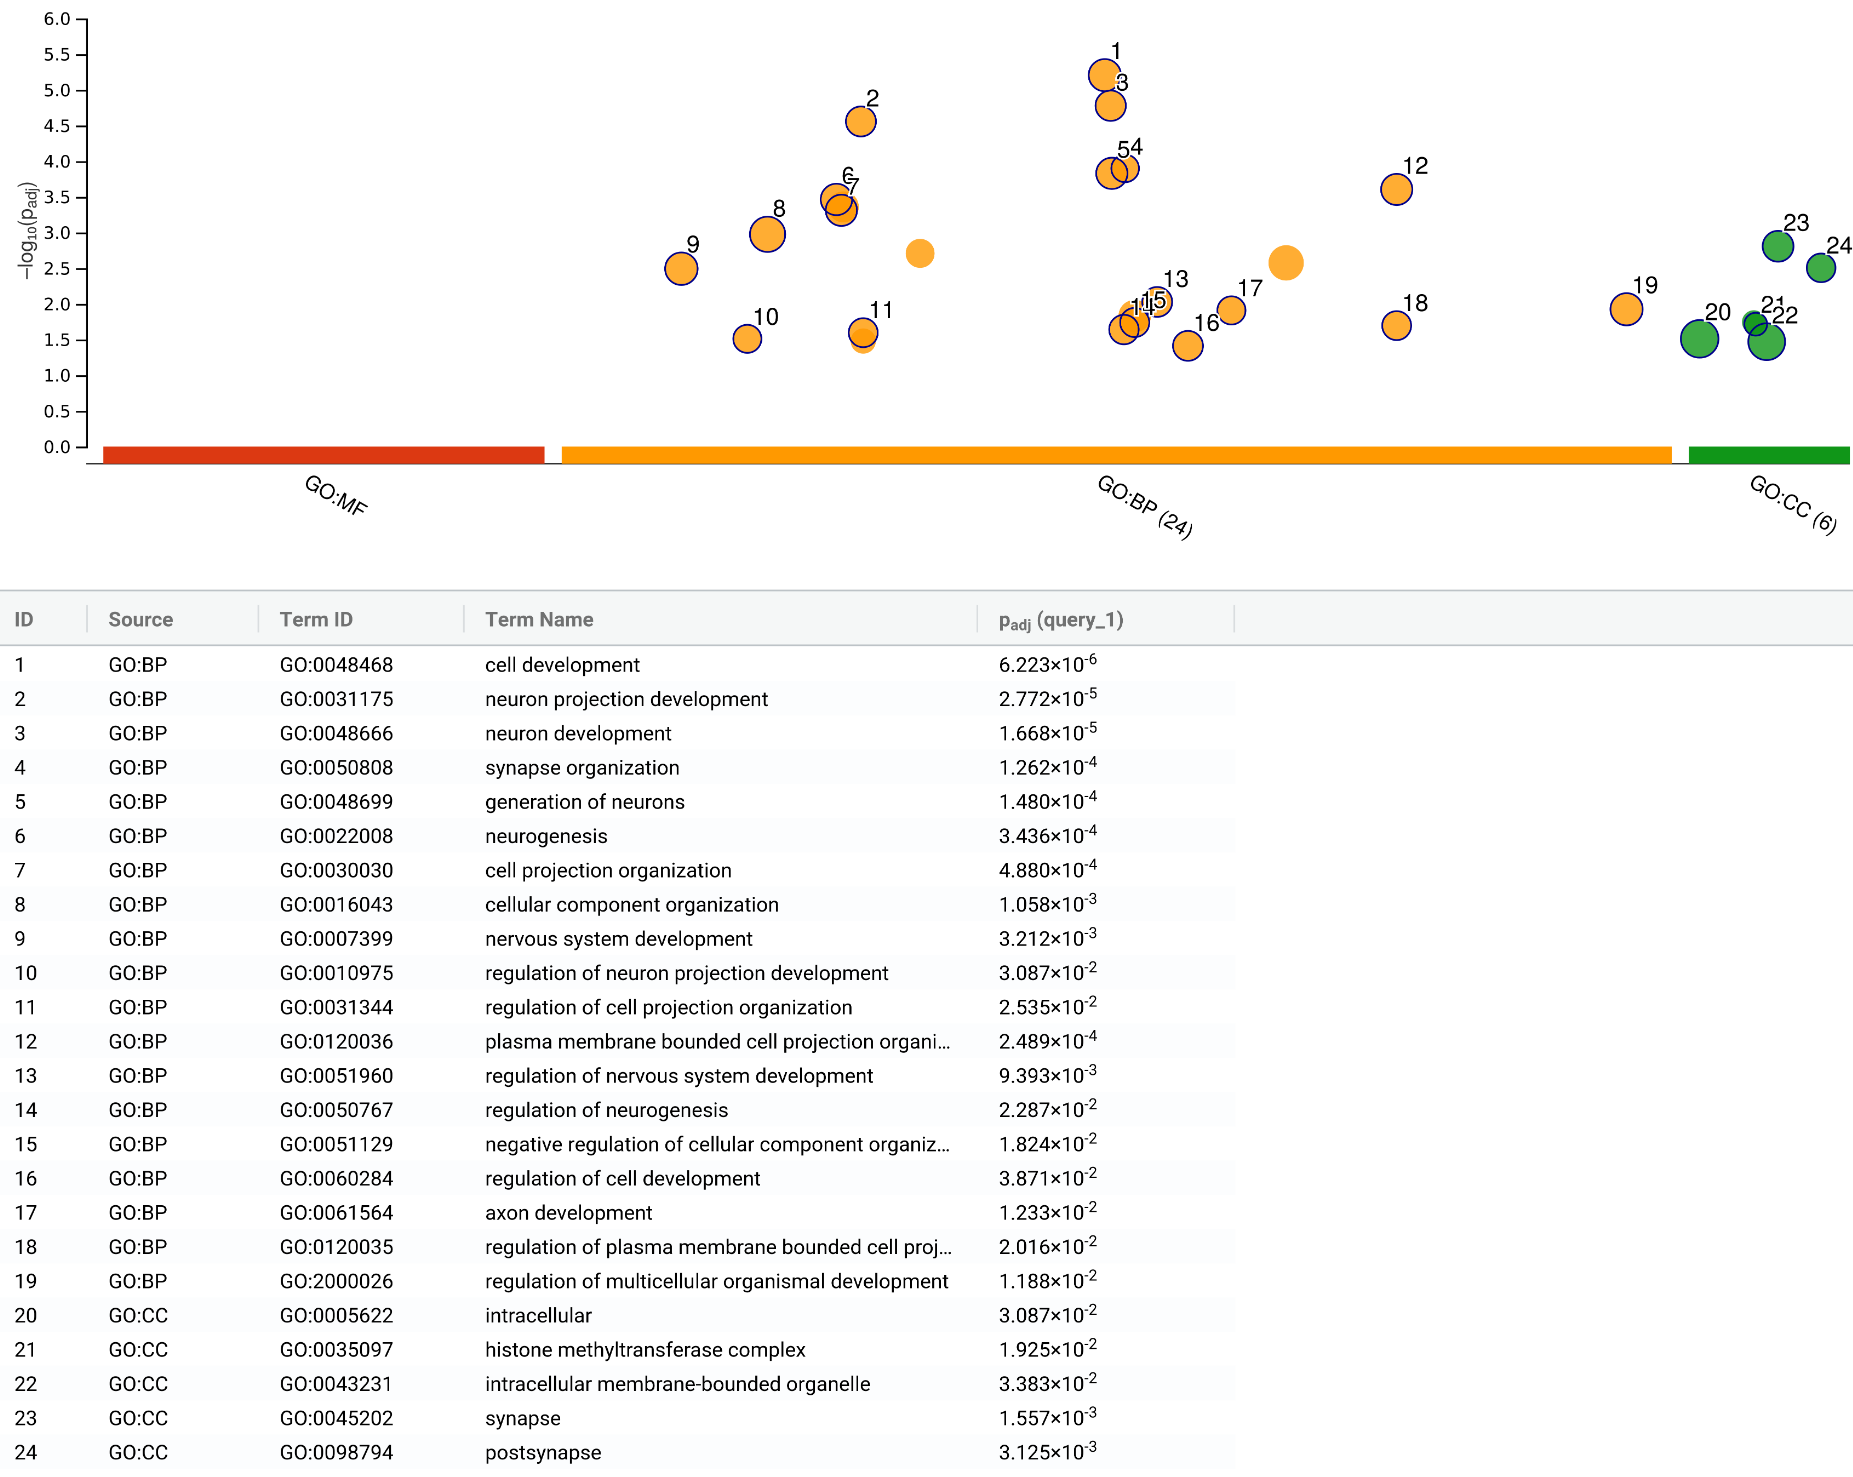
\includegraphics[width=\textwidth]{images/gprofiler/gprofiler_eukbbed_clip.png}
%     \caption{GO enrichment for significant genes using gProfiler multiple testing control SGS. Education\textsubscript{Discovery} sample}
%     \label{fig:gprofiler_ukbbed}
% \end{figure}

% \begin{figure}
%     \centering

%     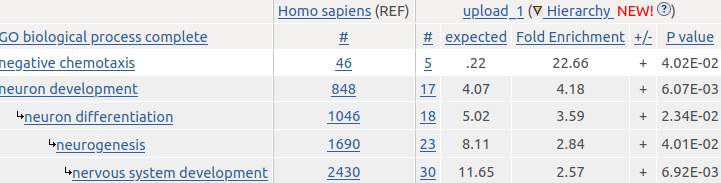
\includegraphics[width=\textwidth]{images/screenshots/EA2_BP_Panther_all_genes_Bonferroni.png}
%     \caption{Education\textsubscript{Replication} Gene Ontology enrichment using PANTHER. Bonferroni correction. Hierarchy of ontology terms shown.}
%     \label{fig:EA2_Panther_BP_Bonf_Hierarchy}
% \end{figure}

% \begin{figure}
%     \centering
%     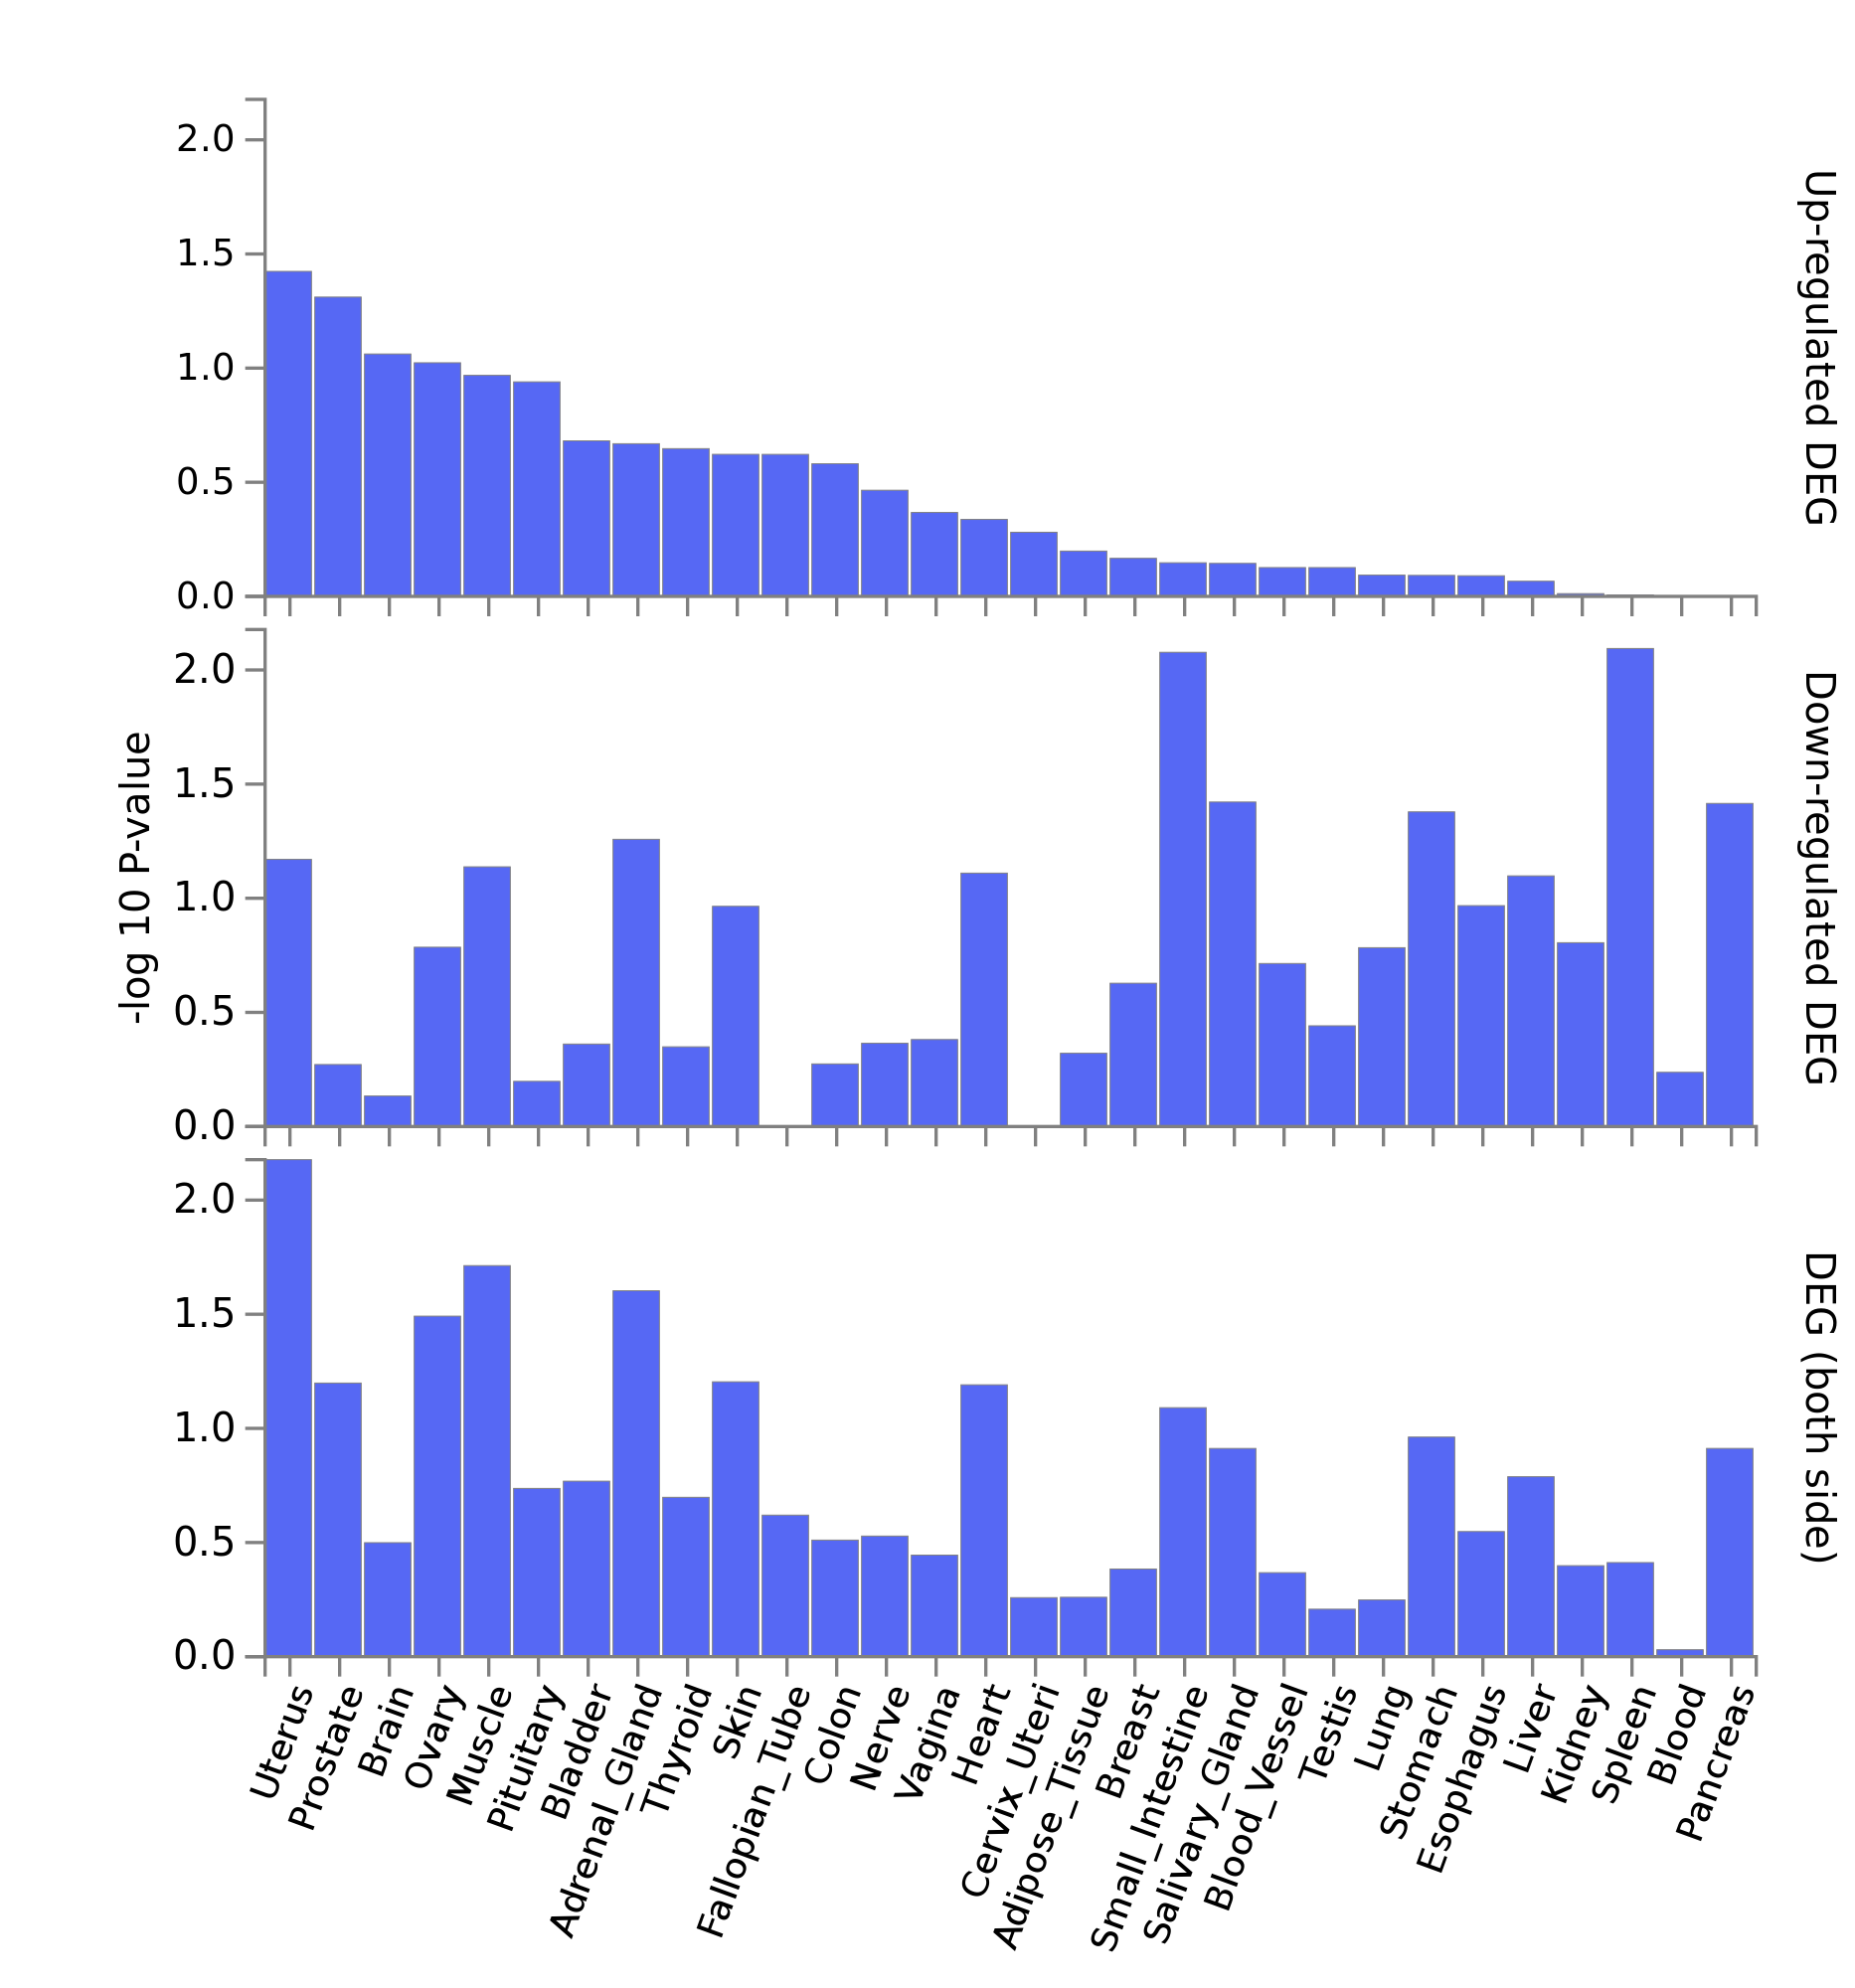
\includegraphics[width=\textwidth]{images/FUMA_plots/gtex_v8_ts_FUMA_30_99_genes.png}
%     \caption{GTEx differential enrichment ordered by upregulated genes in Education\textsubscript{Replication} cohort}
%     \label{fig:GTEX_EA2_DEG}
% \end{figure}



\subsubsection{ToppGene:Results Education\textsubscript{Replication}}

The 99 significant genes were enriched compared to the rest of the genome  using ToppFun and the FDR method, Benjamini and Hochberg (FDR BH) to correct for multiple comparisons. Seventy seven significant terms were found for Biological Process using the FDR method Benjamini and Hochberg (10 with Bonferroni, 22 using FDR Q value Benjamini and Yekutieli, FDR BY). Twenty annotations for cellular component were significantly over represented (2 Bonferroni, 2 FDR BY). No molecular function annotations were found to be enriched in the 99 genes found at GWGAS. Enrichment was performed using default background and settings. 


The significant biological process terms are shown in  table~\ref{tab:BP EA2 all significant toppgene top}. The top two terms are neurogenesis (GO:0022008,q FDR BH= 0.002) and gliogenesis (GO:0042063,q FDR BH= 0.002) both reported by Okbay et al. using DEPICT in an expanded sample\cite{okbay2016genome}. The significant genes are not enriched for molecular function but show enrichment for two cellular component terms, the top being "post synapse" GO:0098794.

Given that differences in significance values have been reported between enrichment packages\cite{khatri2005ontological}(here differences can be seen in the number annotated for identical inputs), I calculated  the correlation of the -log10 transform of the uncorrected p values for the seventeen annotations found in both PANTHER and ToppGene (17 of 19 for PANTHER, 17 of 77 for ToppGene). Pearson's product-moment correlation was 0.594 (95\%CI 0.158-0.84); t=2.861,df=15, p-value= 0.01189 (see figure~\ref{fig:correlation of gene ontology terms between toppgene and panther}). 

\begin{figure}
    \centering
    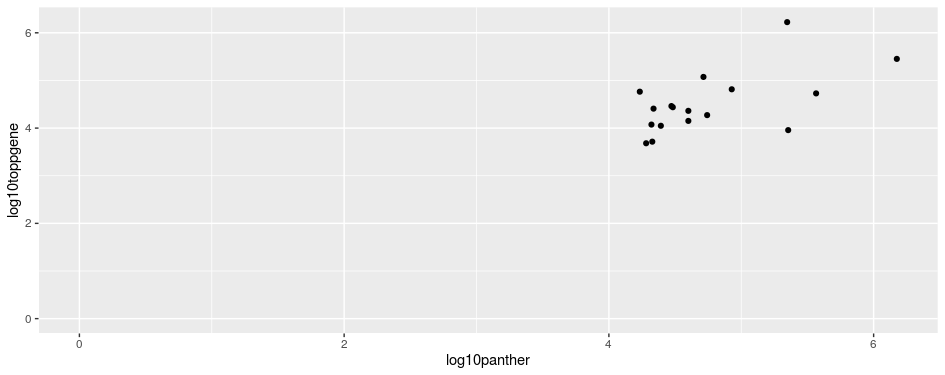
\includegraphics[width=\textwidth]{images/chapter2/strontium/Rplot_compare_toppgene_panther.png}
    \caption{Correlation between gene ontology term enrichment values in ToppGene and PANTHER for Education\textsubscript{Discovery} sample. Scatterplot shows -log10 transform of uncorrected p value for PANTHER on x-axis and -log10 transform of ToppGene values on y axis. There appears to be a linear relationship between the two although the number of samples is small.}
    \label{fig:correlation of gene ontology terms between toppgene and panther}
\end{figure}


% t = 2.8612, df = 15, p-value = 0.01189
% alternative hypothesis: true correlation is not equal to 0
% 95 percent confidence interval:
%  0.1589549 0.8360662
% sample estimates:
%       cor 
% 0.5942021 

% latex table generated in R 3.6.3 by xtable 1.8-4 package
% Mon Sep 21 14:31:22 2020
\begin{table}[ht]
\centering
\begin{adjustbox}{width=\textwidth}

\begin{tabular}{llrrrrrr}
  \hline
ID & Name & p & q Bonf & q BH & q BY & n query & n genome \\ 
  \hline
GO:0022008 & neurogenesis & $5.969 \times 10^{-7}$ & 0.002 & 0.002 & 0.014 & 26 & 1866 \\ 
  GO:0042063 & gliogenesis & $1.143 \times 10^{-6}$ & 0.003 & 0.002 & 0.014 & 11 & 352 \\ 
  GO:0007417 & central nervous system development & $1.812 \times 10^{-6}$ & 0.005 & 0.002 & 0.015 & 19 & 1129 \\ 
  GO:0048666 & neuron development & $3.528 \times 10^{-6}$ & 0.010 & 0.002 & 0.021 & 20 & 1297 \\ 
  GO:0010001 & glial cell differentiation & $5.159 \times 10^{-6}$ & 0.015 & 0.002 & 0.021 & 9 & 261 \\ 
  GO:0050808 & synapse organization & $5.386 \times 10^{-6}$ & 0.016 & 0.002 & 0.021 & 12 & 498 \\ 
  GO:0048667 & cell morphogenesis involved in neuron dif. & $5.919 \times 10^{-6}$ & 0.017 & 0.002 & 0.021 & 14 & 688 \\ 
  GO:0048699 & generation of neurons & $8.435 \times 10^{-6}$ & 0.025 & 0.003 & 0.027 & 23 & 1751 \\ 
  GO:0048812 & neuron projection morphogenesis & $1.389 \times 10^{-5}$ & 0.041 & 0.004 & 0.031 & 14 & 742 \\ 
  GO:0010771 & negative regulation of cell morphogenesis  dif. & $1.534 \times 10^{-5}$ & 0.045 & 0.004 & 0.031 & 6 & 109 \\ 
   \hline
\end{tabular}
\end{adjustbox}
\caption{Top 10 terms biological process Topp Gene Education\textsubscript{Replication}. dif. = involved in differentiation. BH FDR q value Benjaminin and Hochberg, BY FDR Benjamini and Yekutieli, Bonf = Bonferroni, n query = number of genes in sample (GWGAS significant genes in Education\textsubscript{Replication}) annotated to this term, n genome = number of genes in genome annotated to this term \url{source('~/RProjects/paper_xls_output/R/chapter_2/panther_and_toppgene/panther_and_toppgene_ea2.R')}}
~\ref{tab:BP EA2 all significant toppgene top}
\end{table}




% latex table generated in R 3.6.3 by xtable 1.8-4 package
% Mon Sep 21 14:47:23 2020
\begin{table}[ht]
\centering
\begin{adjustbox}{width=\textwidth}
\begin{tabular}{llrrrrrr}
  \hline
ID & Name & p & q Bonf & q BH & q BY & n query & n genome \\ 
  \hline
GO:0098794 & postsynapse & $1.458 \times 10^{-6}$ & 0.001 & 0.001 & 0.003 & 16 & 825 \\ 
  GO:0045202 & synapse & $1.580 \times 10^{-5}$ & 0.005 & 0.003 & 0.018 & 20 & 1482 \\ 
  GO:0005794 & Golgi apparatus & $2.099 \times 10^{-4}$ & 0.073 & 0.015 & 0.097 & 19 & 1643 \\ 
  GO:0097418 & neurofibrillary tangle & $2.178 \times 10^{-4}$ & 0.075 & 0.015 & 0.097 & 2 & 5 \\ 
  GO:0035658 & Mon1-Ccz1 complex & $2.178 \times 10^{-4}$ & 0.075 & 0.015 & 0.097 & 2 & 5 \\ 
  GO:0031252 & cell leading edge & $2.705 \times 10^{-4}$ & 0.094 & 0.016 & 0.100 & 9 & 449 \\ 
  GO:0071458 & integral component of cytoplasmic side of ERM & $3.256 \times 10^{-4}$ & 0.113 & 0.016 & 0.103 & 2 & 6 \\ 
  GO:0044297 & cell body & $4.697 \times 10^{-4}$ & 0.163 & 0.020 & 0.131 & 12 & 820 \\ 
  GO:0036477 & somatodendritic compartment & $6.068 \times 10^{-4}$ & 0.210 & 0.023 & 0.146 & 14 & 1096 \\ 
  GO:0043025 & neuronal cell body & $6.590 \times 10^{-4}$ & 0.228 & 0.023 & 0.146 & 11 & 732 \\ 
   \hline
\end{tabular}
\end{adjustbox}
\caption{ Top 10 Terms Cellular component ToppGene Education\textsubscript{Replication}. ERM=Endoplasmic reticulum membrane BH FDR q value Benjaminin and Hochberg, BY FDR Benjamini and Yekutieli, Bonf = Bonferroni, n query = number of genes in sample (GWGAS significant genes in Education	extsubscript{Replication}) annotated to this term, n genome = number of genes in genome annotated to this term} 
~\ref{tab:CC EA2 all significant toppgene}
\end{table}
% \begin{table}[ht]
% \centering
% \begin{tabular}{rllrrrr}
%   \hline
%  & ID & Name & test & Genome & p & Bon \\ 
%   \hline
% 1 & GO:0022008 & neurogenesis & 26 & 1866 & $5.97 \times 10^{-7}$ & 0.00176 \\ 
%   2 & GO:0042063 & gliogenesis & 11 & 352 & $1.14 \times 10^{-6}$ & 0.00337 \\ 
%   3 & GO:0007417 & central nervous syst & 19 & 1129 & $1.81 \times 10^{-6}$ & 0.00535 \\ 
%   4 & GO:0048666 & neuron development & 20 & 1297 & $3.53 \times 10^{-6}$ & 0.01041 \\ 
%   5 & GO:0010001 & glial cell different & 9 & 261 & $5.16 \times 10^{-6}$ & 0.01522 \\ 
%   6 & GO:0050808 & synapse organization & 12 & 498 & $5.39 \times 10^{-6}$ & 0.01589 \\ 
%   7 & GO:0048667 & cell morphogenesis i & 14 & 688 & $5.92 \times 10^{-6}$ & 0.01747 \\ 
%   8 & GO:0048699 & generation of neuron & 23 & 1751 & $8.43 \times 10^{-6}$ & 0.02489 \\ 
%   9 & GO:0048812 & neuron projection mo & 14 & 742 & $1.39 \times 10^{-5}$ & 0.04100 \\ 
%   10 & GO:0010771 & negative regulation  & 6 & 109 & $1.53 \times 10^{-5}$ & 0.04527 \\ 
%   \hline
% \end{tabular}
% \caption{BP EA2 all significant Toppgene 99 genes in total \url{source('~/RProjects/paper_xls_output/R/chapter_2/eda_toppgene_all_significant_ea2.R')}} 
% \label{tab:BP EA2 all significant toppgene}
% \end{table}


 %$p$ corrected 0.005 (see table~\ref{tab:CC EA2 all significant Toppgene}).
 
 \footnote{Translation of genes for toppgene correct at\url{source('~/RProjects/paper_xls_output/R/chapter_2/FUMA/edit_gene_table/EA2_FUMA2clipboard.R')} all 99.
  Entrez ID from MAGMA to symbol to edited symbols. (Correct)}
 
  
% \todo{CHANGE IMPORTANT}
\paragraph{SynGO}

Sixteen genes were annotated ontology terms using SynGO and over representation was carried out using a background set, for which 1104 genes are SynGO annotated genes. The results are shown in table~\ref{tab:enrichment of gene ontology terms in syngo}. The terms are more significant, with lower raw p values, due to a smaller background set (1104 SynGO annotated genes) and a decreased number of terms. 

\paragraph{g:Profiler}

One molecular function term, two cellular component terms and eight biological process terms were found to be significant after corrections for multiple comparisons using the g:SCS method (see section~\ref{sec:gProfiler GO enrichment}). The two cellular component terms are the same as those discovered using ToppGene with the Bonferroni or Benjamini-Yekutieli methods for multiple comparisons (synapse and post synapse). Synapse organisation (GO:0050808) is the most enriched biological process term (p adjusted g:SCS $5.78\times10^{-4}$). Terms related to neurogenesis (GO:0022008) p adjusted = 0.0154) and neuron projection development (GO:0031175, p adjusted g:SCS=0.0024) are enriched as reported by Okbay et al\cite{okbay2016genome} using DEPICT (see figure~\ref{fig:gProfiler EA2}).



\begin{figure}
    \centering
    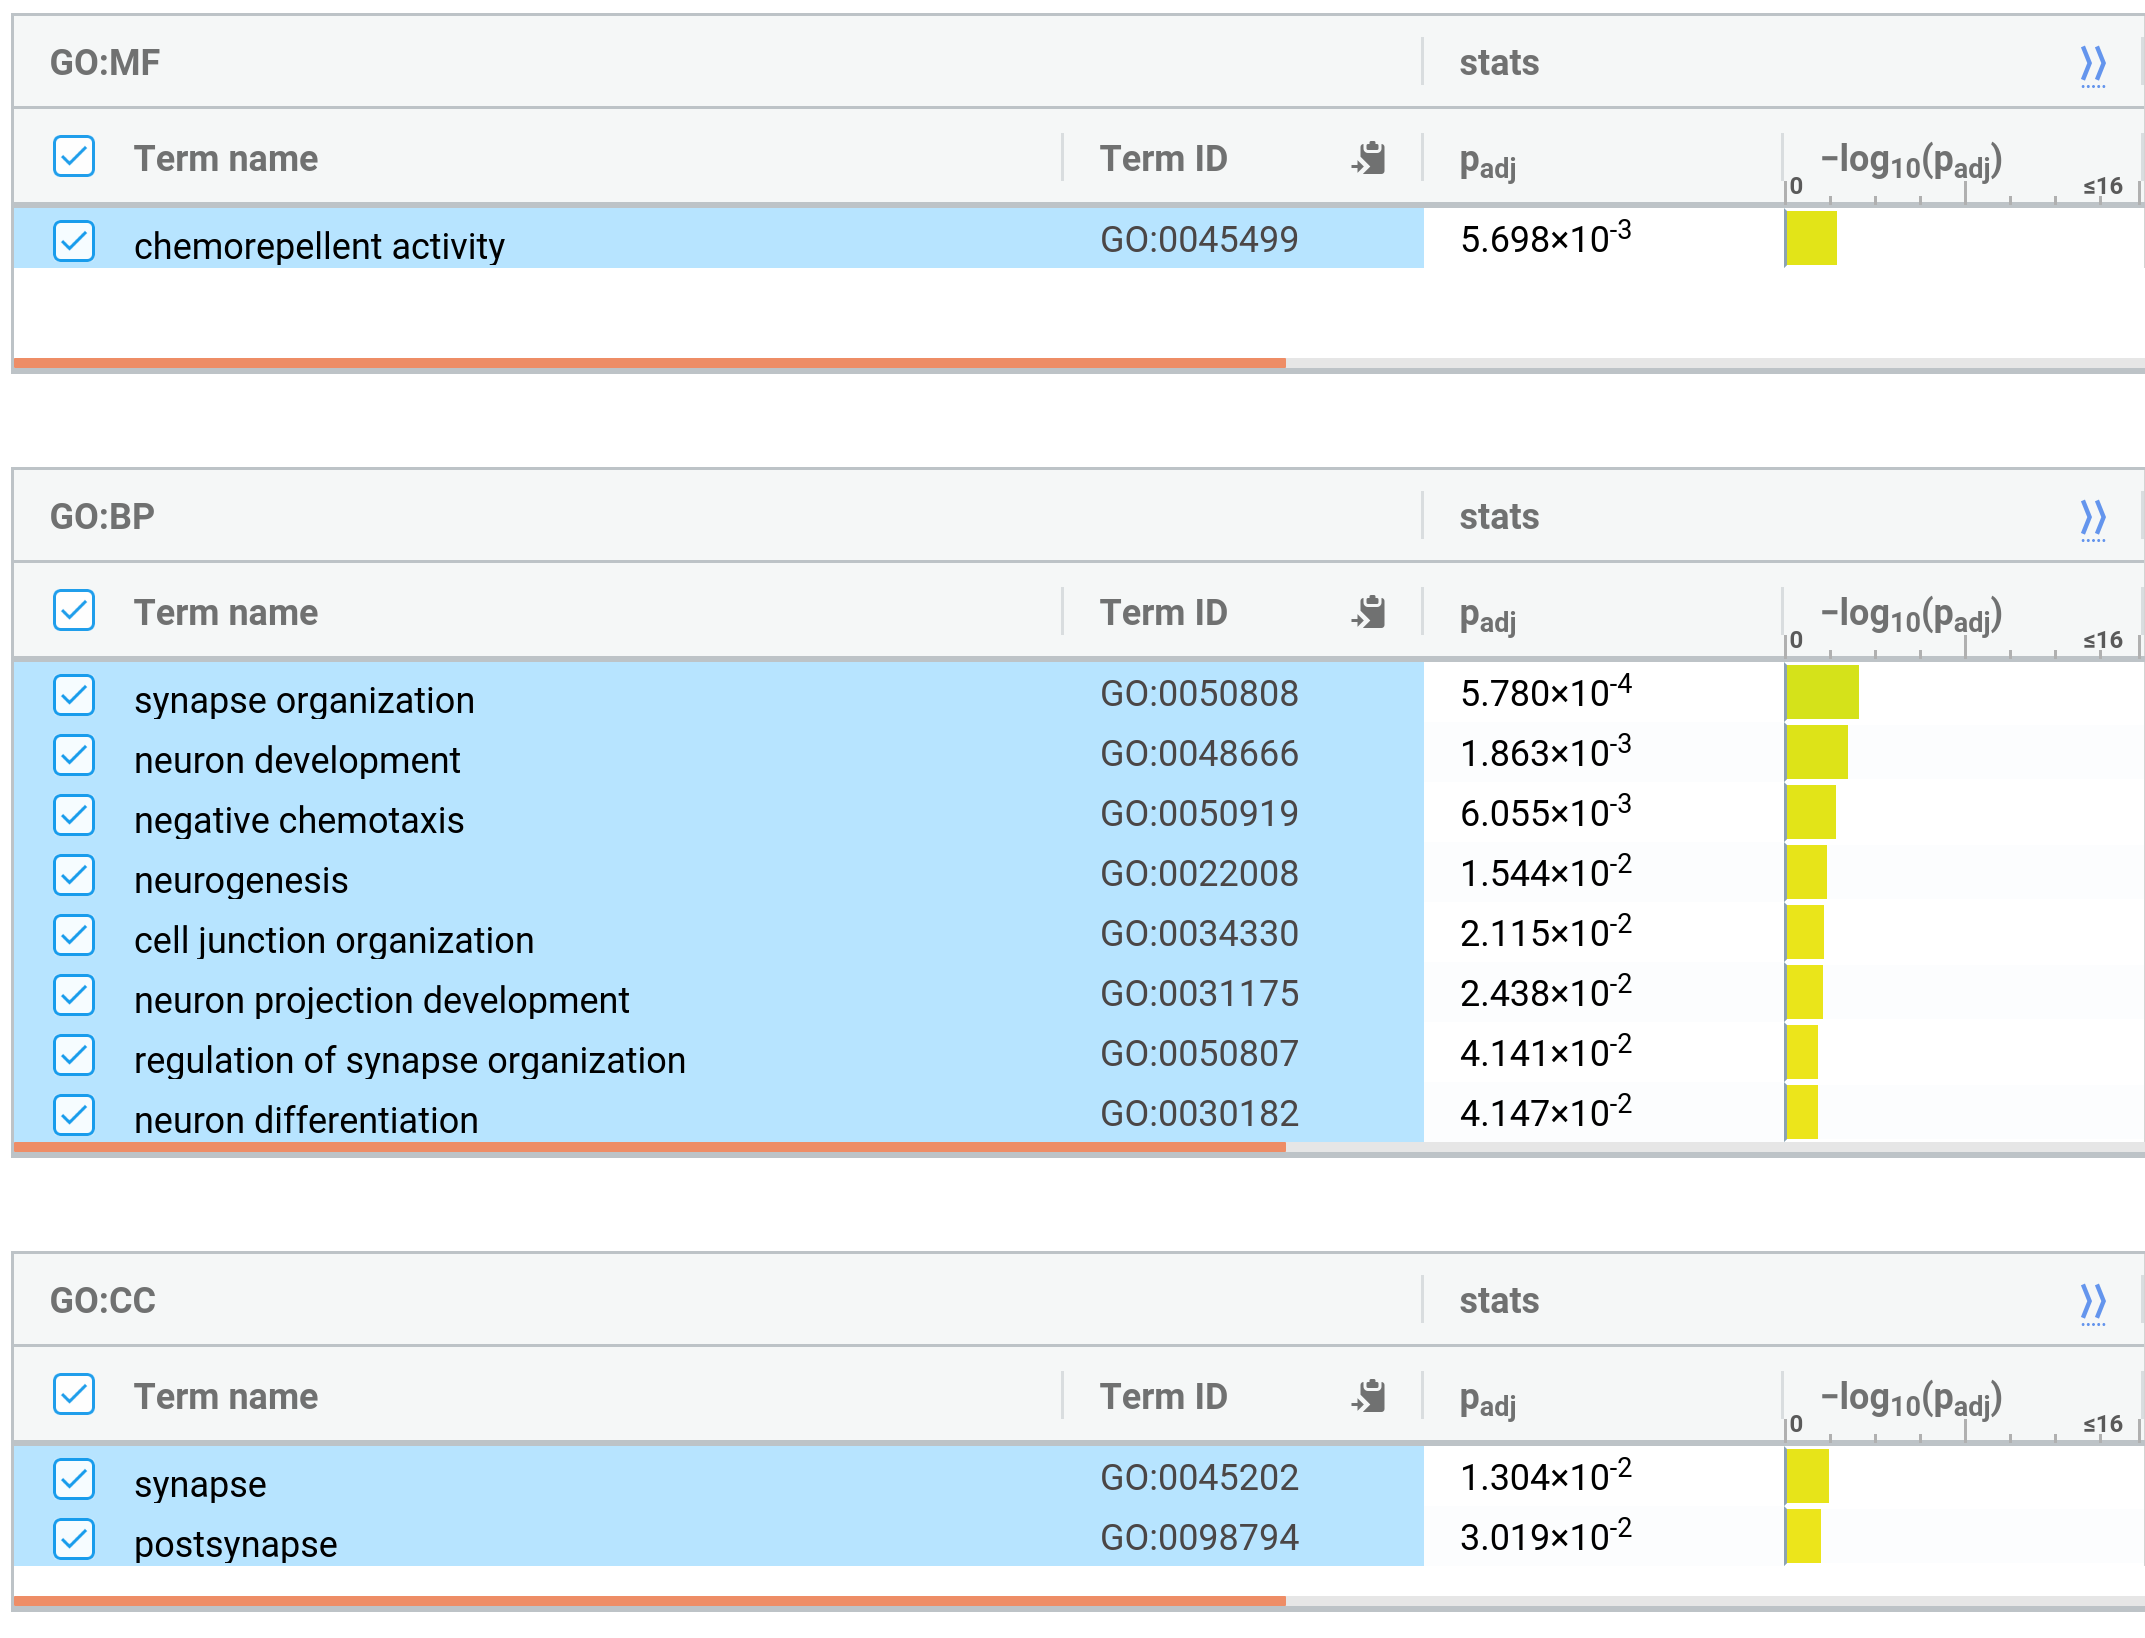
\includegraphics[width=\textwidth]{images/gprofiler/all_terms/ea2_all_terms.png}
    \caption{gProfiler Education\textsubscript{Replication}}
    \label{fig:gProfiler EA2}
\end{figure}

% Dataset name
% ea
% ID mapping
% 16 / 99 (unique) genes from your gene list were mapped to SynGO annotated genes.
% Settings
% experimental-evidence filtering is not enabled (default setting)
% Genes
% 14 genes have a Cellular Component annotation, 13 for Biological Processes. Note: a gene may have multiple annotations.
% Annotations
% 18 annotations against a Cellular Component, 25 for Biological Processes.
% Enrichment
% 1 Cellular Component terms are significantly enriched at 1% FDR (testing terms with at least three matching input genes), 4 for Biological Processes.
% Background
% "brain expressed" background set was selected, contains 18035 unique genes in total of which 1104 overlap with SynGO annotated genes.
% Readme commented out





\begin{table}[]
    \centering
    \begin{tabular}{llll}
    Biological Process & n & p & FDRq\\
    \hline
synapse organization*&	12&	6.94e-8	&3.47e-7\\
process in the synapse&	13&	4.14e-4	&1.03e-3\\
regulation of synapse organization	&3&	6.98e-4&	1.16e-3\\
synapse adhesion between pre- and post-synapse&	3	&1.35e-3&	1.68e-3\\
trans-synaptic signaling	&3	&0.0644&	0.0644\\
\\
 Cellular component & n & p & FDRq\\
 \hline
    synapse&14	&8.68e-4	&3.47e-3\\
postsynapse&	9	&5.40e-3	&0.0108       \\
         
\end{tabular}
    \caption{Enrichment of Gene Ontology terms using SynGO. SynGO only tests for biological process and cellular comparment. FDR q = adjusted significance level using FDR. Note the increased significance level despite correcting for multiple comparisons. For term Synapse Organisation (GO:0050808)* 12 genes (including child terms) in annotation, 286 in SynGO. }
    \label{tab:enrichment of gene ontology terms in syngo}
\end{table}
% SynGO data downloaded on 2020-9-8 12:2 @ https://www.syngoportal.org
% SynGO dataset version/release: 20180731

% Summary of your gene list
% ea
% 26 / 233 (unique) genes from your gene list were mapped to SynGO annotated genes.
% experimental-evidence filtering is not enabled (default setting)
% 23 genes have a Cellular Component annotation, 20 for Biological Processes. Note: a gene may have multiple annotations.
% 32 annotations against a Cellular Component, 39 for Biological Processes.
% 0 Cellular Component terms are significantly enriched at 1% FDR (testing terms with at least three matching input genes), 1 for Biological Processes.
% "brain expressed" background set was selected, contains 18035 unique genes in total of which 1104 overlap with SynGO annotated genes.

% "user_genelist_map_to_syngo_genes.xlsx" contains your input genelist (first column) together with the matching gene ID available in SynGO. If your input could not be matched to any SynGO annotated gene, the latter will be empty.
% "syngo_annotations_matching_user_input.xlsx" contains all available SynGO annotations that match your input genelist.
% "syngo_ontologies_with_annotations_matching_user_input.xlsx" contains all SynGO ontology terms, together with the Gene Set Enrichment Analysis (GSEA) results and all genes from these terms that match your input genelist.

% The JSON folder contains data in a format convenient for bioinformatic analysis.

% The SynGO_geneset_CC/BP.json files contain all SynGO annotated genes for each synaptic ontology term. On the first level of this nested list you can find 'direct' and 'aggregate' annotations, you will want to use the latter for geneset analyses as these contain (for each term) both the annotated genes for an ontology term and all genes annotated against (recursive) child terms. For instance, in the aggregate dataset the term 'presynapse' also contains all genes annotated against its child term 'active zone'. Further, note that we originally mapped the annotated proteins from various species to HGNC identifiers. The ensembl/entrez/MGI/RGD mappings (from HGNC ID) in these JSON files were provided by the genenames.org webservice, so if you focus on Ensembl genes consider mapping the HGNC IDs to the exact Ensembl build that you are using.

  \paragraph{Disease Enrichment}
  
  Disease enrichment in DisGeNet BeFree\cite{pinero2020disgenet} searched by ToppFun (part of the ToppGene suite) is found for intellectual disability (ID:C3714756) which is the top term. Twenty genes are found from 1219 in the annotation ($p=8.88\times10^{-7}$, FDR BH=0.00165). Intellectual disability was reported to be enriched by Okbay et al \cite{okbay2016genome} for a larger related sample using DEPICT. Six of the genes are found in the PSP (See fig~\ref{tab:Intellectual disability genes significant in EA2 found in PSP} for intellectual disability associated genes significant at GWGAS in Education\textsubscript{Replication} sample. ) Testing enrichment with PSP as background found no significantly enriched disease terms other than inflammatory bowel disease. (See supplemental material)\footnote{Enrichment in DisGeNet BeFree searched by toppfun of Intellectual disabilityID C3714756 	Intellectual Disability ; Source	DisGeNET BeFree ; p 	8.884E-7 ; FDR BH	1.648E-3; FR BY 	1.386E-2 ;Bonferroni	2.237E-3; Input 	20 	Total 1219}.See fig~\ref{tab:Intellectual disability genes significant in EA2 found in PSP} for intellectual disability associated genes significant at GWGAS in Education\textsubscript{Replication} sample. 
        % latex table generated in R 3.6.3 by xtable 1.8-4 package
        
% Sun Aug 23 12:35:02 2020
\begin{table}[ht]
\centering
\begin{tabular}{lll}
  \hline
Entrez Gene ID & Gene Symbol & Gene Name \\
  \hline
5144 & PDE4D & phosphodiesterase 4D  \\
  5662 & PSD & pleckstrin and Sec7 domain containing \\
  
  4137 & MAPT & microtubule associated protein tau \\ 
  4208 & MEF2C & myocyte enhancer factor 2C \\ 
  4744 & NEFH & neurofilament heavy \\
  257194 & NEGR1 & neuronal growth regulator 1 \\ 
   \hline
\end{tabular}
\caption{Intellectual disability genes significant in Education\textsubscript{Replication} genes found at GWGAS EA2 found in PSP.} 
\label{tab:Intellectual disability genes significant in EA2 found in PSP}
\end{table}
 
%  ToppFun with background PSP (new)
%  No GO terms
%  No phenotype
%  (4 out of 5 inflammatory bowel are in PSP)
        
        % GTEx
\subsection{Intelligence\textsubscript{Discovery} Ontology enrichment}


Gene set analysis of this sample, combined with the Intelligence\textsubscript{Discovery} sample and augmented by educational attainment data using MTAG is reported by Hill et al.  \cite{hill2019combined}. MAGMA GSA was carried out using 10,891 gene sets from Gene ontology, Reactome and MSigDB and using the Bonferroni correction for multiple comparisons (raw p required = 0.05/10891 = $4.59 \times 10^{-6}$)\footnote{Actual footnote: Bonferroni $\alpha$ from supplementary table 5 $2.75\times10^{-6}$
 which I calculate as 18182 comparisons the same as the correction for multiple comparisons in the gene level statistics. The paper however says a correction of 10891 which I calculate means the corrections is $4.59\times10^{-6}$. This does not however result in any extra significant sets.  27 gene sets are obtained using the FDR correction }. GSA revealed 8 quite large gene sets\footnote{See \url{source('~/RProjects/chapter2_checks/R/expected_gsa/ctg_size_plots.R')} for correlation between raw p value and gene size.} including neurogenesis (1355 genes) and genes associated with the synapse (717 genes), regulation of nervous system development (722 genes), neuron projection (989 genes), neuron differentiation (842 genes), CNS neuron differentiation (160 genes) and cell development (808 genes) (see table~\ref{tab:MAGMA GSA results from Hill et al.}). 


\begin{table}[ht]
\centering
\begin{tabular}{lrrrr}
  \hline
Gene set name & N genes in gene set & Beta & SE($\beta$) & p \\ 
  \hline
Neurogenesis  & 1355 & 0.20 & 0.05 & $5.59 \times 10^{-10}$ \\ 
  Regulation of nervous system development  & 722 & 0.23 & 0.05 & $4.02 \times 10^{-8}$ \\ 
  Regulation of cell development  & 808 & 0.22 & 0.04 & $7.38 \times 10^{-8}$ \\ 
  Neuron projection  & 898 & 0.20 & 0.04 & $2.07 \times 10^{-7}$ \\ 
  Central nervous system neuron differentiation  & 160 & 0.47 & 0.04 & $5.33 \times 10^{-7}$ \\ 
  Synapse  & 717 & 0.21 & 0.04 & $1.43 \times 10^{-6}$ \\ 
  Neuron differentiation  & 842 & 0.19 & 0.04 & $1.62 \times 10^{-6}$ \\ 
  Oligodendrocyte differentiation  & 1037 & 0.17 & 0.04 & $1.75 \times 10^{-6}$ \\ 
   \hline
\end{tabular}
\caption{MAGMA GSA significant sets from Hill et al. 2019 Bonferroni $\alpha$ from supplementary table 5 $2.75\times10^{-6}$ from \cite{hill2019combined}}
\label{tab:MAGMA GSA results from Hill et al.}
\end{table}

% % latex table generated in R 3.6.3 by xtable 1.8-4 package
% % Tue Sep 15 11:43:35 2020
% \begin{table}[ht]
% \centering
% \begin{tabular}{lrrrr}
%   \hline
% Gene.set.Name & n genes & Beta & SE & p \\ 
%   \hline
% Neurogenesis  & 1355 & 0.20 & 0.05 & $5.59 \times 10^{-10}$ \\ 
%   Regulation of nervous system development  & 722 & 0.23 & 0.05 & $4.02 \times 10^{-8}$ \\ 
%   Regulation of cell development  & 808 & 0.22 & 0.04 & $7.38 \times 10^{-8}$ \\ 
%   Neuron projection  & 898 & 0.20 & 0.04 & $2.07 \times 10^{-7}$ \\ 
%   Central nervous system neuron differentiation  & 160 & 0.47 & 0.04 & $5.33 \times 10^{-7}$ \\ 
%   Synapse  & 717 & 0.21 & 0.04 & $1.43 \times 10^{-6}$ \\ 
%   Neuron differentiation  & 842 & 0.19 & 0.04 & $1.62 \times 10^{-6}$ \\ % latex table generated in R 3.6.3 by xtable 1.8-4 package
% % Tue Sep 15 11:43:35 2020

% \end{tabular}
% \caption{MAGMA GSA significant sets from Hill et al. 2019 Bonferroni $\alpha$ from supplementary table 5 $2.75\times10^{-6}$ from \cite{hill2019combined}}
% \end{table}









\subsubsection{Intelligence Discovery Gene Ontology analysis PANTHER}
A modified list of gene symbols was again used  to ensure registration of genes using PANTHER \footnote{code at \url{source('~/RProjects/paper_xls_output/R/chapter_2/FUMA/edit_gene_table/UKBB_Int_FUMA2clipboard.R')} gene list at supplemental \url{/home/grant/Dropbox/paper_xls_data/Panther/input.txt}}.
% 197 genes - it is actually 196 genes saved actual genes in paperxls on dropbox

% 191 mapped with NCBI symbol
% Using only approved you get 179 (ie a lot of NCBI are not the approved ones)

% 194 uniquely mapped with symbol

% 196 of 192 uniquely mapped with hgnc id ie all are uniquely mapped and there are multiples but they are all there
% \url{source('~/RProjects/paper_xls_output/R/chapter_2/translate_sig_genes/ukbbint_NCBI_translate2.R')}\footnote{have put stop in at end of script and also there is function to toppgene which needs remov}
% Checked this again this is best using HGNC
% other is \url{source('~/RProjects/paper_xls_output/R/chapter_2/FUMA/edit_gene_table/UKBB_Int_FUMA2clipboard.R')}
% may find more DNA binding with this above 194 terms of 195

% This is confused the correct one is this one which uses gene symbol
% \url{source('~/RProjects/paper_xls_output/R/chapter_2/FUMA/edit_gene_table/UKBB_Int_FUMA2clipboard.R')}
% 11 missing using ENSG annotations
% Gene ID 3 unmapped
% GeneID:100132074 FOXO6
% GeneID:9753
% GeneID:3107

% MGEA5   OGA
% C10orf76    ARMH3
% CCDC101 SGF29
% PET112 GATB
% HIST1H3C H3C3 one of 25 synonyms
% HIST1H3I HIST1H3J one of 24 synonyms
% BAI1 ADGRB1 ADRGB1 Entrez to panther to id
% RP5-874C20.3 pseudogene entrz 7741 ZSCAN26 Entrez to panther to id\footnote{\url{source('~/RProjects/paper_xls_output/R/chapter_2/FUMA/edit_gene_table/UKBB_Int_FUMA2clipboard.R')}}

Only one biological process term was enriched: GO:0010468, regulation of gene expression (p=$4.78\times10^{-6}$, FDR BH=0.038; n in annotation 4907, n in set = 74). 
Seven molecular function terms were enriched the most specific and smallest being DNA binding GO:0003677 (n in annotation 2506, test 48, $p=1.01\times10^{-6}$ FDR=0.0016 (table~\ref{tab:GO molecular function complete Intelligence Discovery FDRover represenation only}))
\begin{table}[ht]
\centering
\begin{tabular}{llrrrrrr}
  \hline
GO & description & Ref & Test & E & Fold & P & FDR \\ 
  \hline
GO:0003677 & DNA binding  & 2506 & 48 & 23.1 & 2.08 & $1.01 \times 10^{-6}$ & 0.0016 \\ 
  GO:0003676 & nucleic acid binding  & 4034 & 64 & 37.1 & 1.72 & $5.51 \times 10^{-6}$ & 0.0052 \\ 
  GO:1901363 & heterocyclic compound binding  & 5999 & 83 & 55.2 & 1.50 & $2.73 \times 10^{-5}$ & 0.0185 \\ 
  GO:0097159 & organic cyclic compound binding  & 6086 & 83 & 56.0 & 1.48 & $4.27 \times 10^{-5}$ & 0.0254 \\ 
  GO:0005515 & protein binding  & 14109 & 159 & 129.9 & 1.22 & $3.77 \times 10^{-6}$ & 0.0045 \\ 
  GO:0005488 & binding  & 16469 & 174 & 151.7 & 1.15 & $2.39 \times 10^{-5}$ & 0.0190 \\ 
  GO:0003674 & molecular\_function  & 18321 & 188 & 168.7 & 1.11 & $9.41 \times 10^{-7}$ & 0.0022 \\ 
   \hline
\end{tabular}
\caption{GO molecular function complete Intelligence Discovery FDR over representation only shown.  Ref=reference set, test:number of genes being tested present in ontology term, E=expected number of genes, Fold= Fold change, P = raw p value, FDR = false discovery rate Benjamini and Hochberg. The most enriched term is DNA binding and all of the annotations are large (smallest is 2506 genes). \url{source('~/RProjects/paper_xls_output/R/chapter_2/make_PANTHER_tables/UKBB_int/make_Panther_table_GO_col_nounderFDR_int.R')}} 
\label{tab:GO molecular function complete Intelligence Discovery FDRover represenation only}
\end{table}

Twenty three cellular component terms were enriched. "DNA packaging complex" is the most enriched term using FDR BH 85 terms in annotation, 9 appear in the significant genes found at GWGAS, (GO:0044815), FDR=0.0002. The second most enriched term is the child term nucleosome, GO:000786, FDR 0.0007 (see figure~\ref{fig:UKBiobank int significant genes at GWGAS. PANTHER GO enrichment Cellular component. FDR correction. Screenshot for hierarchy} and table~\ref{tab:GO cellular component complete Intelligence Discovery FDRover represenation only}). Twenty seven genes (from 1383) are enriched for the cellular component term synapse (GO:0045202;FDR 0.0199).
% \paragraph{MF}   3 terms most significant is Very general term GO:0003677 DNA binding 0.0067 p Bonf 0.0029 p FDR Fold change 2.02

% latex table generated in R 3.6.3 by xtable 1.8-4 package
% Tue Sep 15 17:42:51 2020


\begin{figure}
    \centering
    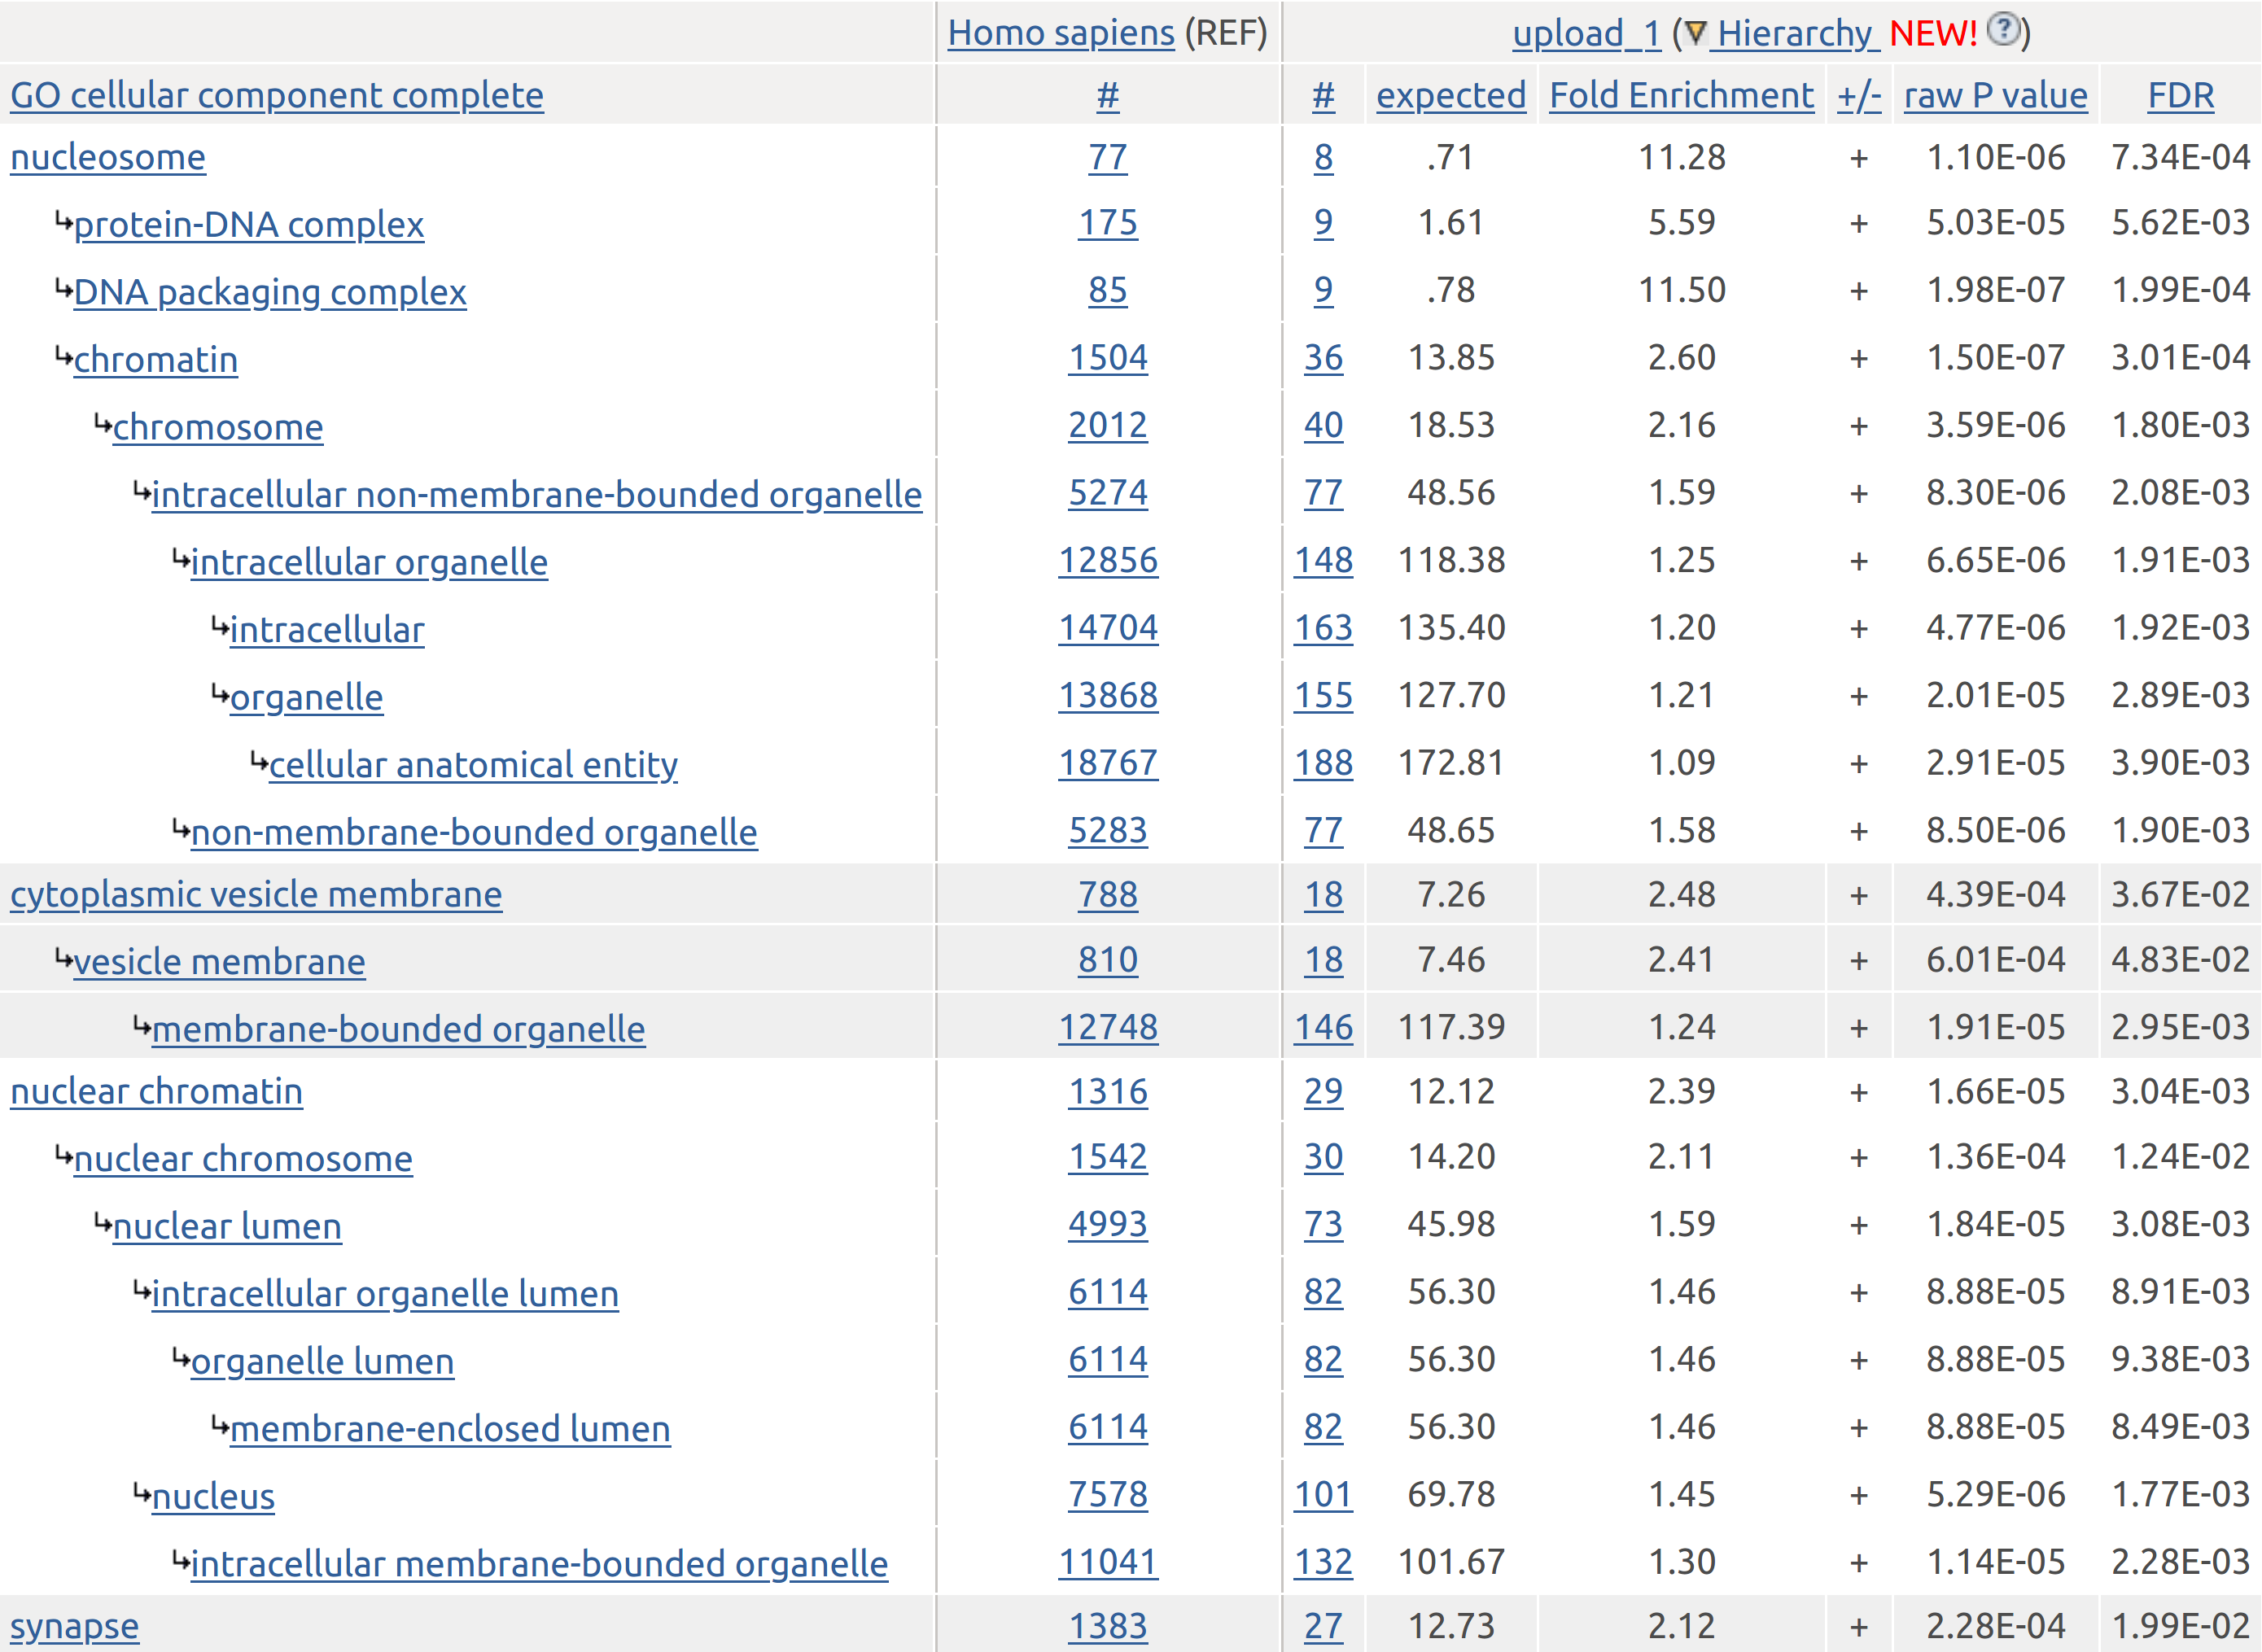
\includegraphics[width=\textwidth]{images/chapter2/strontium/ukbbint_cc.png}
        \caption{UKBiobank intelligence significant genes at GWGAS. PANTHER GO enrichment Cellular component. FDR correction. Screenshot for hierarchy. Matches table check table~\ref{tab:GO cellular component complete Intelligence Discovery FDRover represenation only} }
    \label{fig:UKBiobank int significant genes at GWGAS. PANTHER GO enrichment Cellular component. FDR correction. Screenshot for hierarchy}
\end{figure}

%Removed table tab:GO molecular function complete Intelligence Discovery FDRover represenation only replaces more accurate id changes

% latex table generated in R 3.6.3 by xtable 1.8-4 package
% Sun Aug 30 16:02:36 2020
% \begin{table}[ht]
% \centering
% \begin{tabular}{llrrrrrr}
%   \hline
% GO  & description MF & Ref & Test & E & Fold & P & FDR \\ 
%   \hline
% GO:0003677 & DNA binding  & 2486 & 47 & 23.2 & 2.02 & $2.350 \times 10^{-6}$ & 0.003 \\ 
%   \hspace{2mm}GO:0003676 & \hspace{2mm}nucleic acid binding  & 4024 & 63 & 37.6 & 1.67 & $1.630 \times 10^{-5}$ & 0.015 \\ 
%   \hspace{4mm}GO:0097159 & organic cyclic compound binding  & 6075 & 83 & 56.8 & 1.46 & $7.060 \times 10^{-5}$ & 0.042 \\ 
%   \hspace{4mm}GO:1901363 & heterocyclic compound binding  & 5987 & 83 & 56.0 & 1.48 & $4.490 \times 10^{-5}$ & 0.030 \\ 
  
%   GO:0005515 & protein binding  & 14110 & 162 & 132.0 & 1.23 & $2.070 \times 10^{-6}$ & 0.003 \\ 
   
% %   GO:0003674 & molecular\_function  & 18318 & 191 & 171.3 & 1.11 & $6.440 \times 10^{-7}$ & 0.002 \\ 
% %   UNCLASSIFIED & Unclassified  & 2533 & 4 & 23.7 & 0.17 & $6.440 \times 10^{-7}$ & 0.003 \\ 
%   \hline
% \end{tabular}
% \caption{GO molecular function complete Intelligence\textsubscript{Discovery} FDR over represenation only  Ref reference set, test:number of genes being tested present in ontology termE expected number of genes being tested present in ontology term, Fold= Fold change, = raw p value, FDR = false discovery rate} 
% \label{tab:GO molecular function complete Intelligence DIscovery FDRover represenation only}
% \end{table}



% \paragraph{CC}

% latex table generated in R 3.6.3 by xtable 1.8-4 package
% Tue Sep 15 17:39:45 2020

\begin{table}[ht]
\centering
\begin{adjustbox}{width=\textwidth}

\begin{tabular}{llrrrrrr}
  \hline
GO & description & Ref & Test & E & Fold & P & FDR \\ 
  \hline
GO:0044815 & DNA packaging complex  & 85 & 9 & 0.8 & 11.50 & $1.98 \times 10^{-7}$ & 0.0002 \\ 
  GO:0000786 & nucleosome  & 77 & 8 & 0.7 & 11.28 & $1.10 \times 10^{-6}$ & 0.0007 \\ 
  GO:0032993 & protein-DNA complex  & 175 & 9 & 1.6 & 5.59 & $5.03 \times 10^{-5}$ & 0.0056 \\ 
  GO:0000785 & chromatin  & 1504 & 36 & 13.8 & 2.60 & $1.50 \times 10^{-7}$ & 0.0003 \\ 
  GO:0030659 & cytoplasmic vesicle membrane  & 788 & 18 & 7.3 & 2.48 & $4.39 \times 10^{-4}$ & 0.0367 \\ 
  GO:0012506 & vesicle membrane  & 810 & 18 & 7.5 & 2.41 & $6.01 \times 10^{-4}$ & 0.0483 \\ 
  GO:0000790 & nuclear chromatin  & 1316 & 29 & 12.1 & 2.39 & $1.66 \times 10^{-5}$ & 0.0030 \\ 
  GO:0005694 & chromosome  & 2012 & 40 & 18.5 & 2.16 & $3.59 \times 10^{-6}$ & 0.0018 \\ 
  GO:0045202 & synapse  & 1383 & 27 & 12.7 & 2.12 & $2.28 \times 10^{-4}$ & 0.0199 \\ 
  GO:0000228 & nuclear chromosome  & 1542 & 30 & 14.2 & 2.11 & $1.36 \times 10^{-4}$ & 0.0124 \\ 
  GO:0031981 & nuclear lumen  & 4993 & 73 & 46.0 & 1.59 & $1.84 \times 10^{-5}$ & 0.0031 \\ 
  GO:0043232 & intracellular non-membrane-bounded organelle  & 5274 & 77 & 48.6 & 1.59 & $8.30 \times 10^{-6}$ & 0.0021 \\ 
  GO:0043228 & non-membrane-bounded organelle  & 5283 & 77 & 48.6 & 1.58 & $8.50 \times 10^{-6}$ & 0.0019 \\ 
  GO:0043233 & organelle lumen  & 6114 & 82 & 56.3 & 1.46 & $8.88 \times 10^{-5}$ & 0.0094 \\ 
  GO:0070013 & intracellular organelle lumen  & 6114 & 82 & 56.3 & 1.46 & $8.88 \times 10^{-5}$ & 0.0089 \\ 
  GO:0031974 & membrane-enclosed lumen  & 6114 & 82 & 56.3 & 1.46 & $8.88 \times 10^{-5}$ & 0.0085 \\ 
  GO:0005634 & nucleus  & 7578 & 101 & 69.8 & 1.45 & $5.29 \times 10^{-6}$ & 0.0018 \\ 
  GO:0043231 & intracellular membrane-bounded organelle  & 11041 & 132 & 101.7 & 1.30 & $1.14 \times 10^{-5}$ & 0.0023 \\ 
  GO:0043229 & intracellular organelle  & 12856 & 148 & 118.4 & 1.25 & $6.65 \times 10^{-6}$ & 0.0019 \\ 
  GO:0043227 & membrane-bounded organelle  & 12748 & 146 & 117.4 & 1.24 & $1.91 \times 10^{-5}$ & 0.0029 \\ 
  GO:0043226 & organelle  & 13868 & 155 & 127.7 & 1.21 & $2.01 \times 10^{-5}$ & 0.0029 \\ 
  GO:0005622 & intracellular  & 14704 & 163 & 135.4 & 1.20 & $4.77 \times 10^{-6}$ & 0.0019 \\ 
  GO:0110165 & cellular anatomical entity  & 18767 & 188 & 172.8 & 1.09 & $2.91 \times 10^{-5}$ & 0.0039 \\ 
  GO:0005575 & cellular\_component  & 18951 & 189 & 174.5 & 1.08 & $3.56 \times 10^{-5}$ & 0.0045 \\ 
  UNCLASSIFIED & Unclassified  & 1900 & 3 & 17.5 & 0.17 & $3.56 \times 10^{-5}$ & 0.0042 \\ 
   \hline
\end{tabular}
\end{adjustbox}
    \caption{GO cellular component complete Intelligence Discovery FDRover represenation only  Ref reference set, test:number of genes being tested present in ontology termE expected number of genes being tested present in ontology term, Fold= Fold changeP = raw p value, FDR = false discovery rate\url{source('~/RProjects/paper_xls_output/R/chapter_2/make_PANTHER_tables/UKBB_int/make_Panther_table_GO_col_nounderFDR_int.R')}Checked GR 20/09/20} 
\label{tab:GO cellular component complete Intelligence Discovery FDRover represenation only}
\end{table}
% % Sun Aug 30 16:17:46 2020
% \begin{table}[ht]
% \centering
% \begin{tabular}{llrrrrll}
%   \toprule
% GO ID& Description & Ref & Test & E & Fold & P & FDR \\ 
%   \midrule
%     GO:0000786 & nucleosome  & 77 & 8 & 0.7 & 11.11 & $1.23 \times 10^{-6}$ & 0.0012 \\ 
%   \hspace{2mm}\ding{213}  GO:0032993 & protein-DNA complex  & 175 & 9 & 1.6 & 5.50 & $5.67 \times 10^{-5}$ & 0.0095 \\ 
%  \hspace{2mm}\ding{213}  GO:0044815 & DNA packaging complex  & 85 & 9 & 0.8 & 11.32 & $2.26 \times 10^{-7}$ & 0.0005 \\ 

%   \hspace{2mm}\ding{213}   GO:0000785 & chromatin  & 1229 & 25 & 11.5 & 2.18 & $3.29 \times 10^{-4}$ & 0.0472 \\ 
%   \hspace{4mm}\ding{221}   GO:0043229 & intracellular organelle  & 12843 & 150 & 120.1 & 1.25 & $7.58 \times 10^{-6}$ & 0.0030 \\ 
%   \hspace{6mm}\ding{235}   GO:0005622 & intracellular  & 14693 & 165 & 137.4 & 1.20 & $5.80 \times 10^{-6}$ & 0.0039 \\ 
%   \hspace{6mm}\ding{235}  GO:0043226 & organelle  & 13859 & 157 & 129.6 & 1.21 & $2.35 \times 10^{-5}$ & 0.0059 \\ 
%   \hspace{8mm}\ding{233} GO:0110165 & cellular anatomical entity  & 18761 & 191 & 175.4 & 1.09 & $3.060 \times 10^{-5}$ & 0.0056 \\ 
   
   
%   GO:0031981 & nuclear lumen  & 4786 & 68 & 44.8 & 1.52 & $1.60 \times 10^{-4}$ & 0.0247 \\ 
%   \hspace{2mm}\ding{213} GO:0005634 & nucleus  & 7567 & 102 & 70.8 & 1.44 & $6.21 \times 10^{-6}$ & 0.0031 \\ 
%   \hspace{4mm}\ding{221} GO:0043231 & \makecell{intracellular membrane-bounded\\ organelle}  & 11028 & 134 & 103.1 & 1.30 & $9.470 \times 10^{-6}$ & 0.0032 \\ 
  
  
%   \hspace{6mm}\ding{235} GO:0043227 & membrane-bounded organelle  & 12734 & 148 & 119.1 & 1.24 & $1.620 \times 10^{-5}$ & 0.0046 \\ 
  
 
  
% %   GO:0005575 & cellular\_component  & 18946 & 192 & 177.2 & 1.08 & $2.420 \times 10^{-5}$ & 0.0054 \\ 
  
% %   UNCLASSIFIED & Unclassified  & 1905 & 3 & 17.8 & 0.17 & $2.420 \times 10^{-5}$ & 0.0049 \\ 
%   \bottomrule
% \end{tabular}
% \caption{Gene Ontology Enrichment in PANTHER using cellular component complete for significant genes at GWGAS for Intelligence\textsubscript{Discovery FDR} sample. Over represenation of terms only shown. Indendation shows depth of term in GO DAG, least indented deepest term.   Ref reference set, test:number of genes being tested present in ontology term E expected number of genes being tested present in ontology term, Fold= Fold changeP = raw p value, FDR = false discovery rate,} 
% \label{tab:GO cellular component complete Intelligence Discovery FDRover represenation only}
% \end{table}

% latex table generated in R 3.6.3 by xtable 1.8-4 package
Two SLIM molecular function terms were enriched: transcription factor binding (FDR 0.0145) and DNA binding (FDR 0.0189)
table~\ref{tab:ukbbint mf slim panther} continuing the finding of terms related to transcription.
  	\begin{table}[]
  	    \centering
  	    \begin{tabular}{llllllll}
  	    \toprule
  	GO-Slim Molecular Function &	n annotation & n&		expected 	&fold  &	 P value& 	FDR\\
  	   \midrule
transcription factor binding &	203 &	10& 	1.87 &	5.35  &	2.73E-05 &	1.45E-02\\
DNA binding &	806 &	20& 	7.42& 	2.69& 		7.11E-05& 	1.89E-02\\
\bottomrule
  	    \end{tabular}
  	    \caption{UKBB int MF SLIM PANTHER. n annotation= number of genes in annotation; n= number of significant genes; fold = fold change; FDR = false discovery rate Benjamini and Hochberg}
  	    \label{tab:ukbbint mf slim panther}
  	\end{table}
  	
Eighteen SLIM Biological process terms are over represented figure~\ref{fig:ukbb_int_BP_GO_SLIM} for a screenshot that shows the hierarchy of terms. The terms are again related to transcription, including those related to nucleosome assembly, DNA packaging and those regulating RNA polymerase. No SLIM cellular component was enriched. 

\begin{figure}
    \centering
    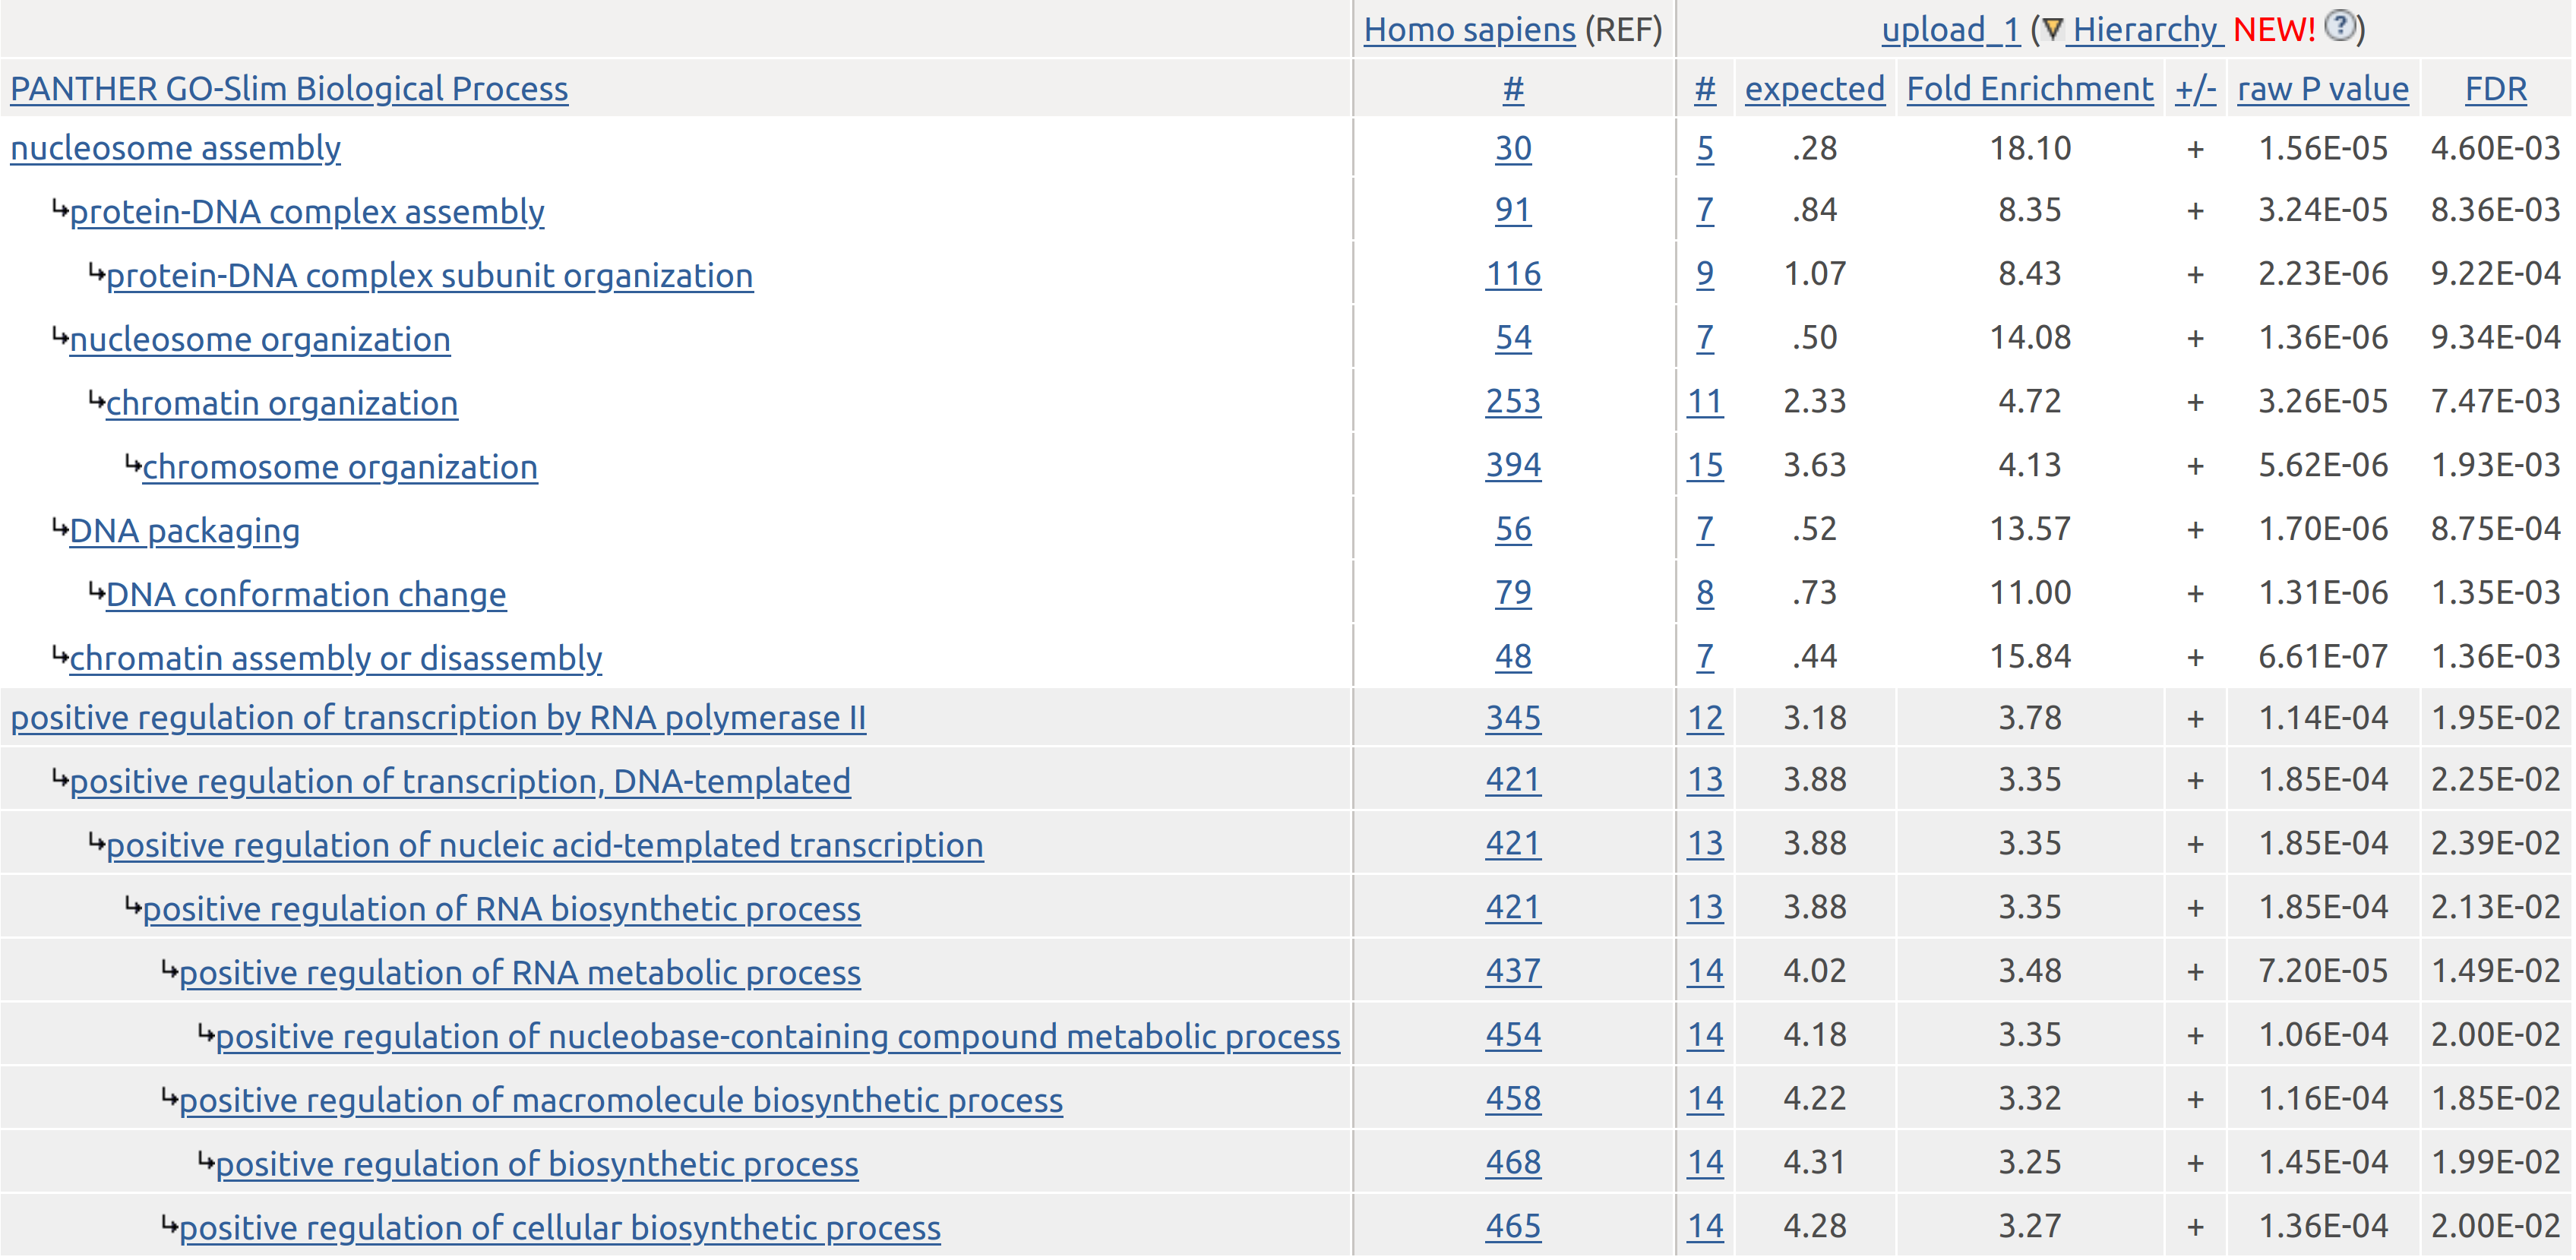
\includegraphics[width=\textwidth]{images/chapter2/large_screenshots/int_discovery_large_bp_slim_panther.png}
    \caption{Int discovery large screenshot BP SLIM. Text file at \url{/home/grant/Dropbox/paper_xls_data/Panther/output_txt/ukbbint/bp_all_slim_checked_with_image_matches_current_image_overleaf.txt}}
    \label{fig:ukbb_int_BP_GO_SLIM}
\end{figure}

PANTHER protein classes were enriched for histone and DNA binding protein (see table~\ref{tab:intelligence discovery panther protein class}.

\begin{table}[]
    \centering
    \begin{tabular}{llllllll}
      PANTHER Protein Class &	n annot & n sample & 	expected& 	Fold &  P & 	FDR\\
      \hline
histone &	55& 	7 &	.51& 	13.82 &	 	1.52E-06 &	2.96E-04\\
DNA binding protein &	227& 	9 &	2.09 &	4.31 &	3.30E-04 &	3.22E-02     \\
         
    \end{tabular}
    \caption{PANTHER protein class enrichment Intelligence\textsubscript{Discovery}}
    \label{tab:intelligence discovery panther protein class}
\end{table}


 Chromatin, RNA polymerase and Pre-Notch expression and processing were among the most enriched of the 98 Reactome pathways tested using PANTHER with 98 terms in total with FDR $<$ 0.05(See figure~\ref{fig:UKBB int topp reac}).
\footnote{table at \url{source('~/RProjects/paper_xls_output/R/chapter_2/make_PANTHER_tables/UKBB_int/make_Panther_table_GO_col_nounderFDRreactome.R')} includes reactome iids}



% \begin{figure}
%     \centering
%     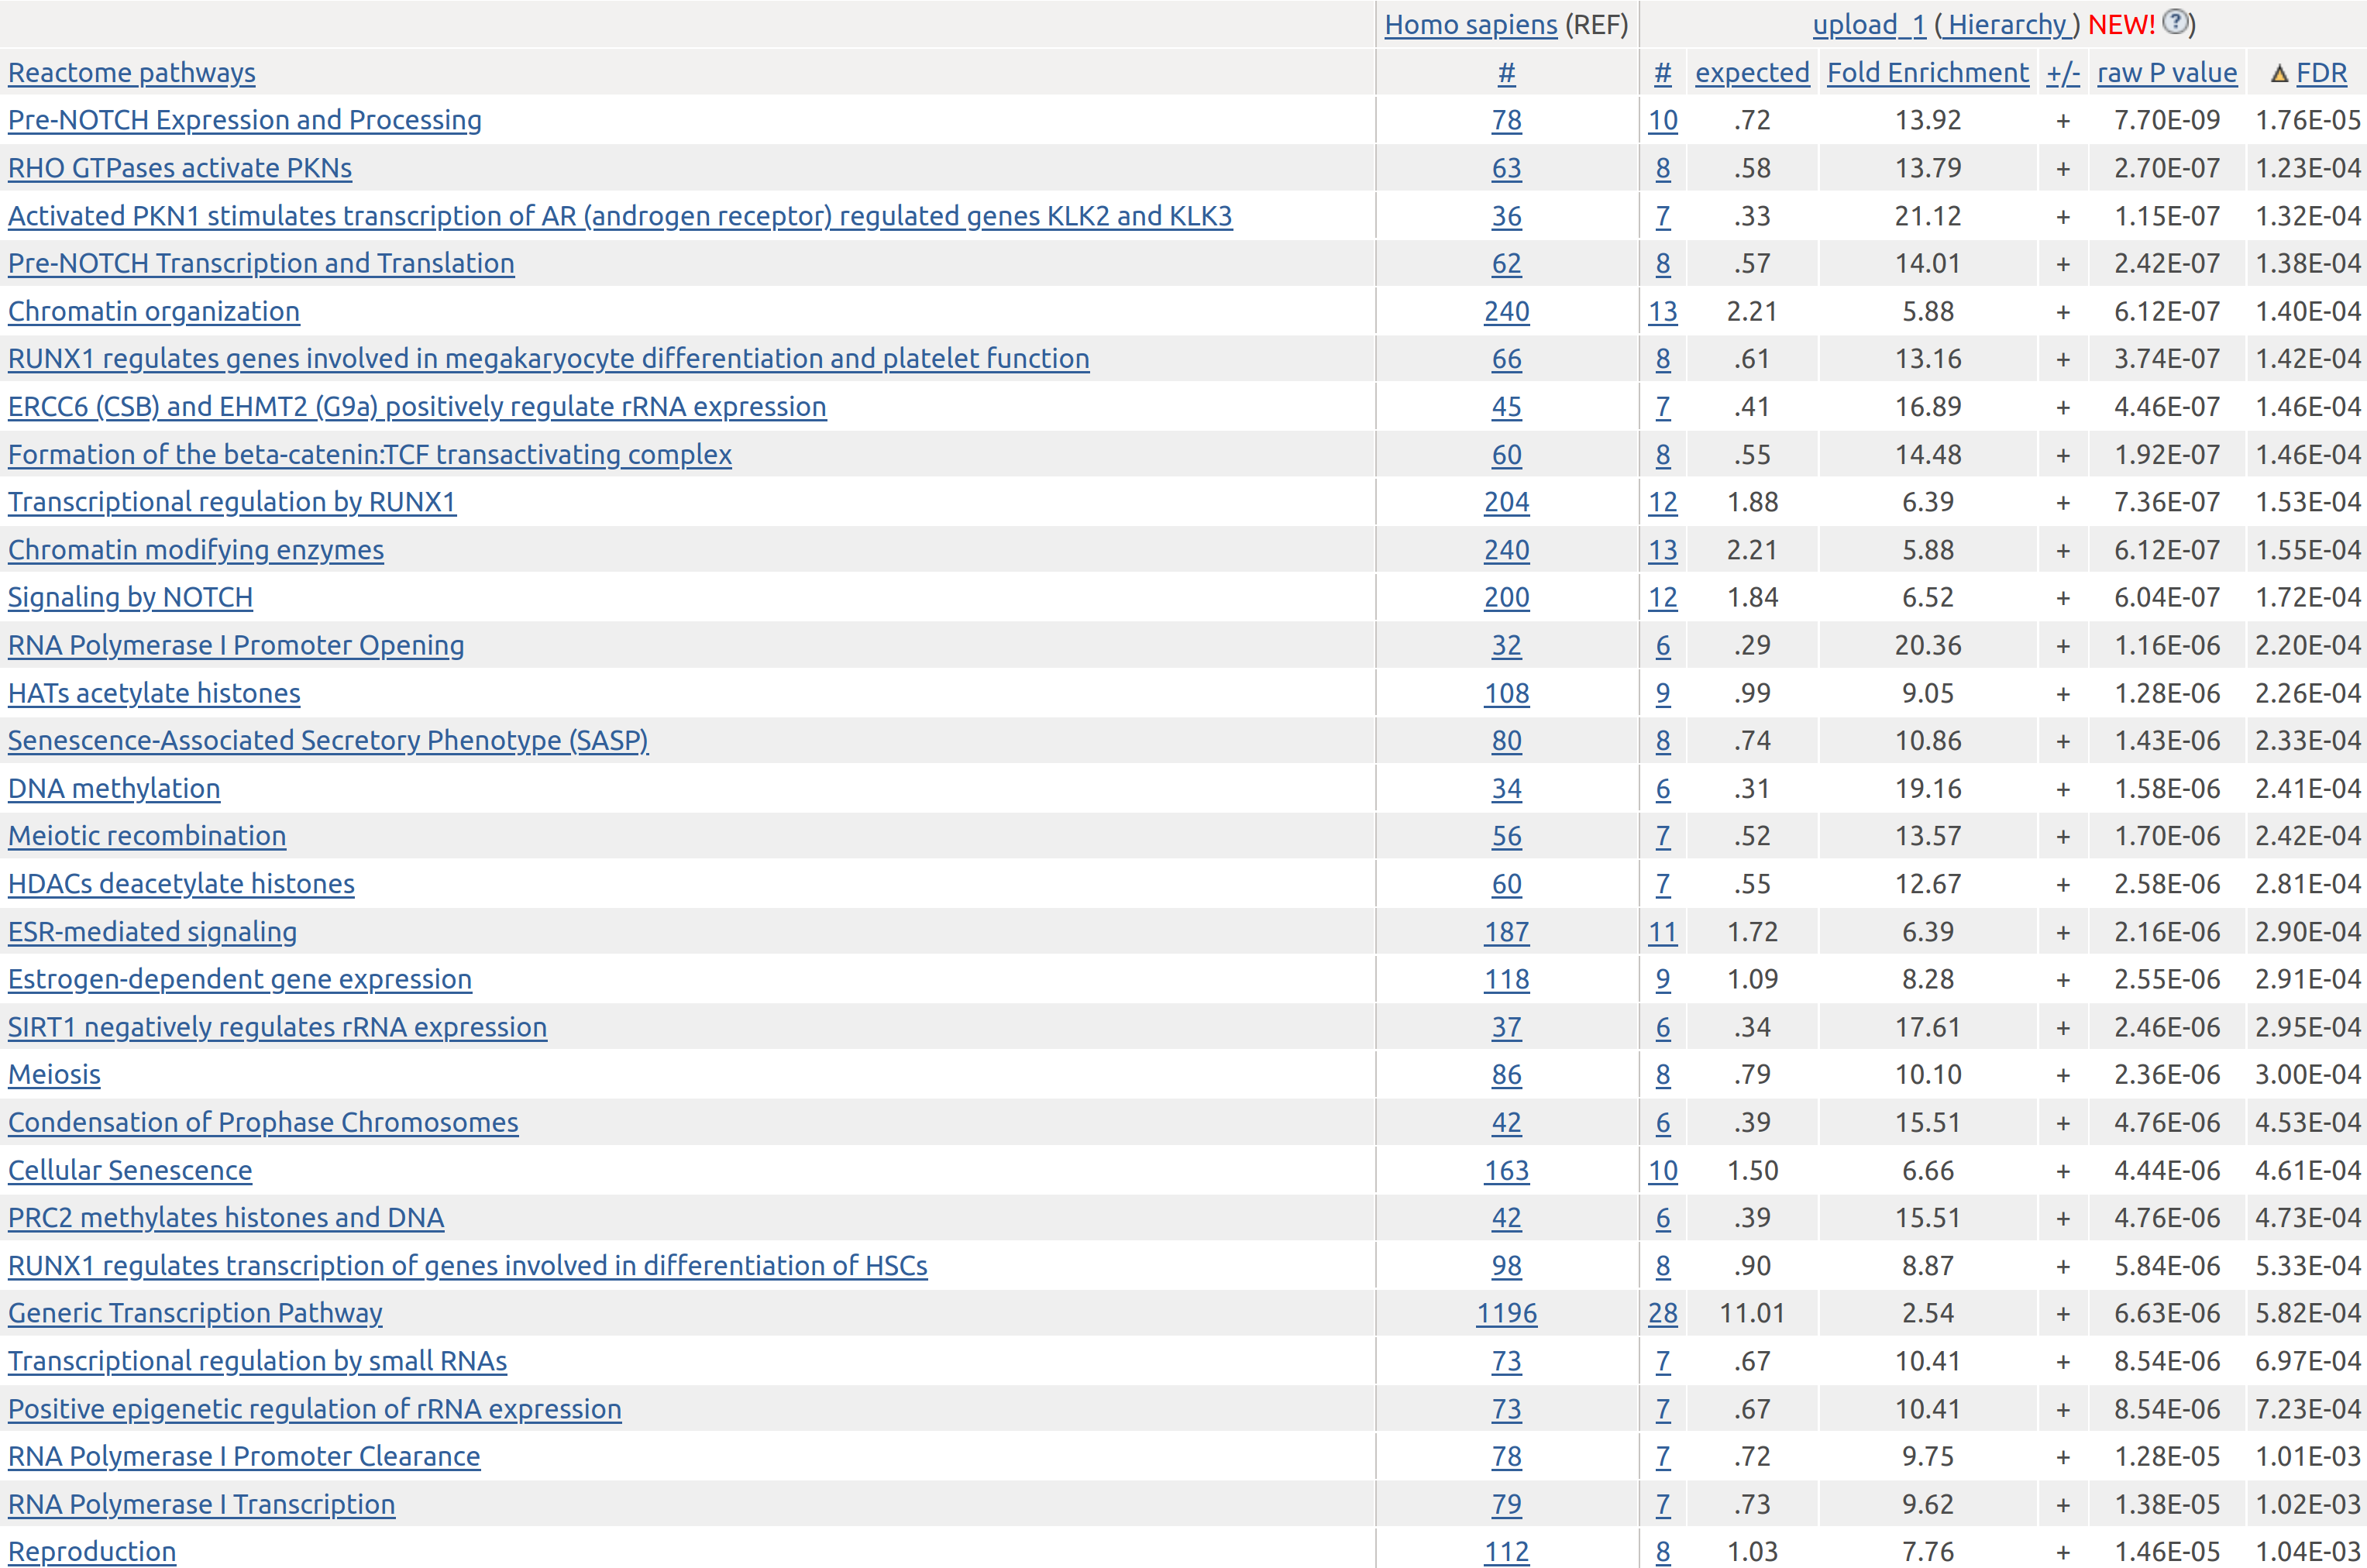
\includegraphics[width=\textwidth]{images/chapter2/large_screenshots/int_discovery_large_reactome_panther1.png}
%     \caption{UKBB int top reactome pathways Panther}
%     \label{fig:UKBB int topp reac}
% \end{figure}

\begin{figure}
    \centering
    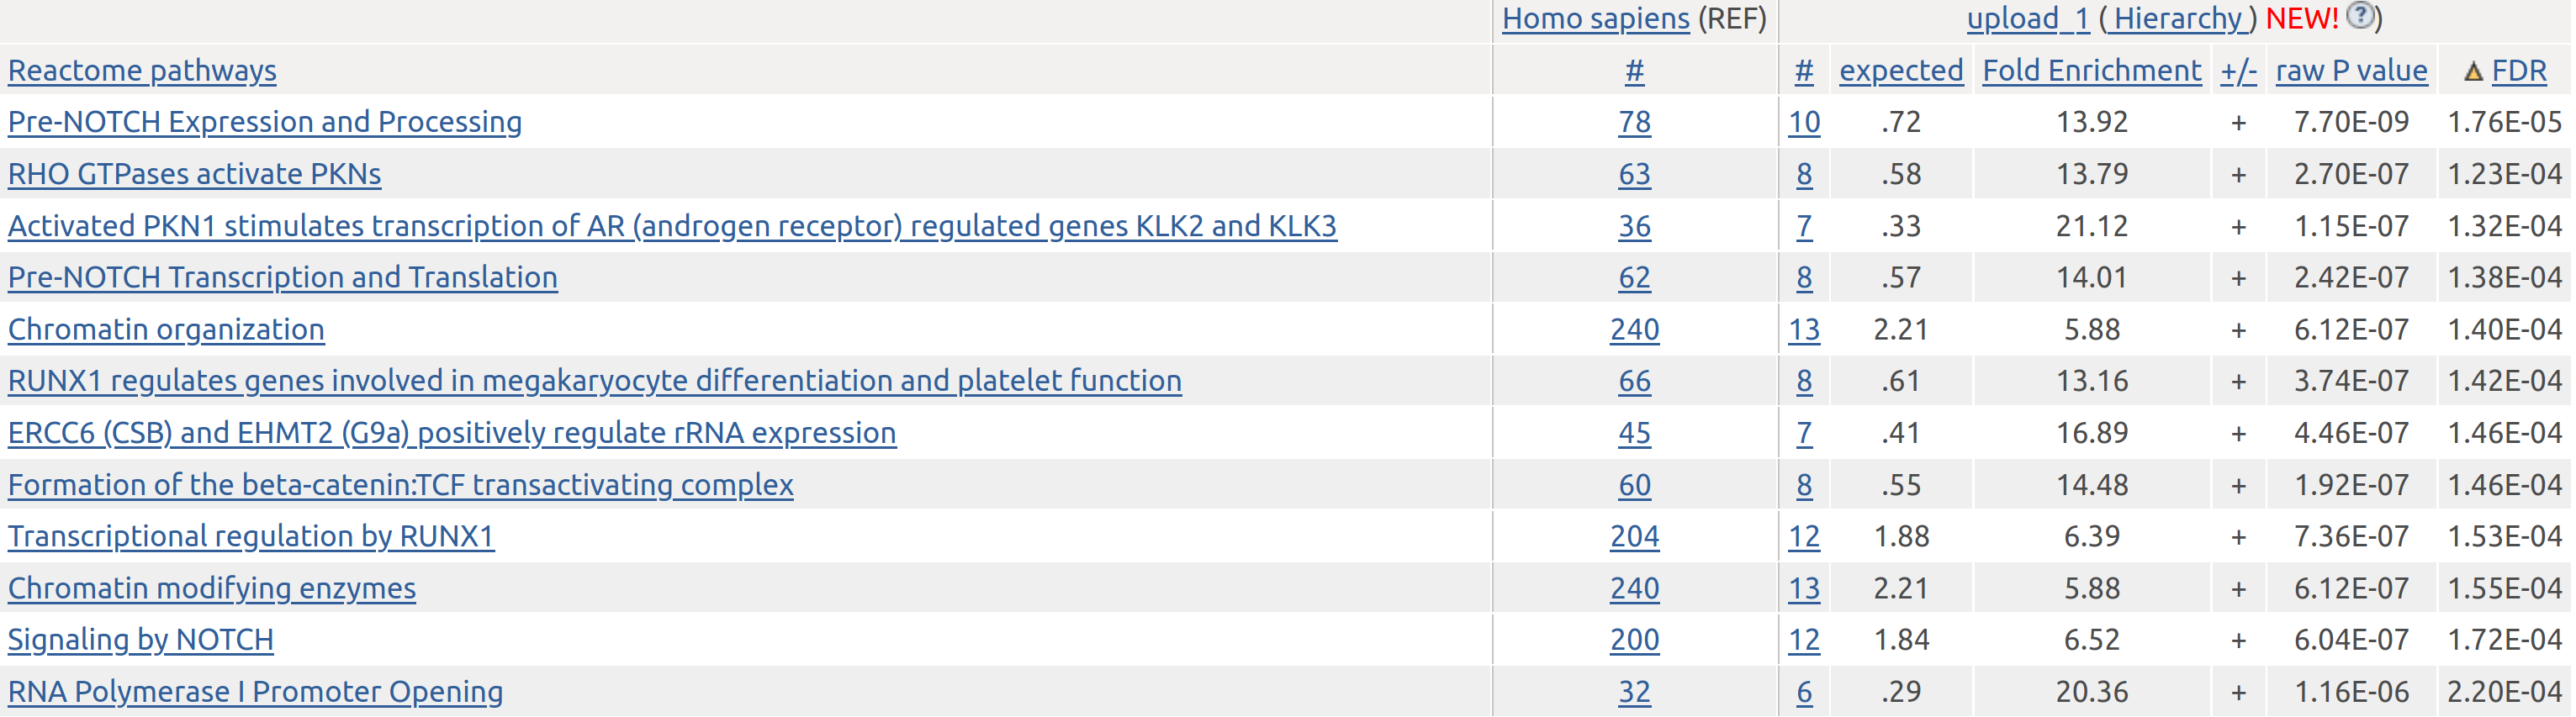
\includegraphics[width=\textwidth]{images/chapter2/large_screenshots/int_discovery_large_reactome_panther3.png}
    \caption{UKBB int top reactome pathways PANTHER}
    \label{fig:UKBB int topp reac}
\end{figure}

g:Profiler results are shown in figure~\ref{fig:gprofiler intelligence discovery} and are a good summary of the main sources of enrichment found in ToppGene and PANTHER (Transcription related and nucleosome assembly). 

\begin{figure}
    \centering
    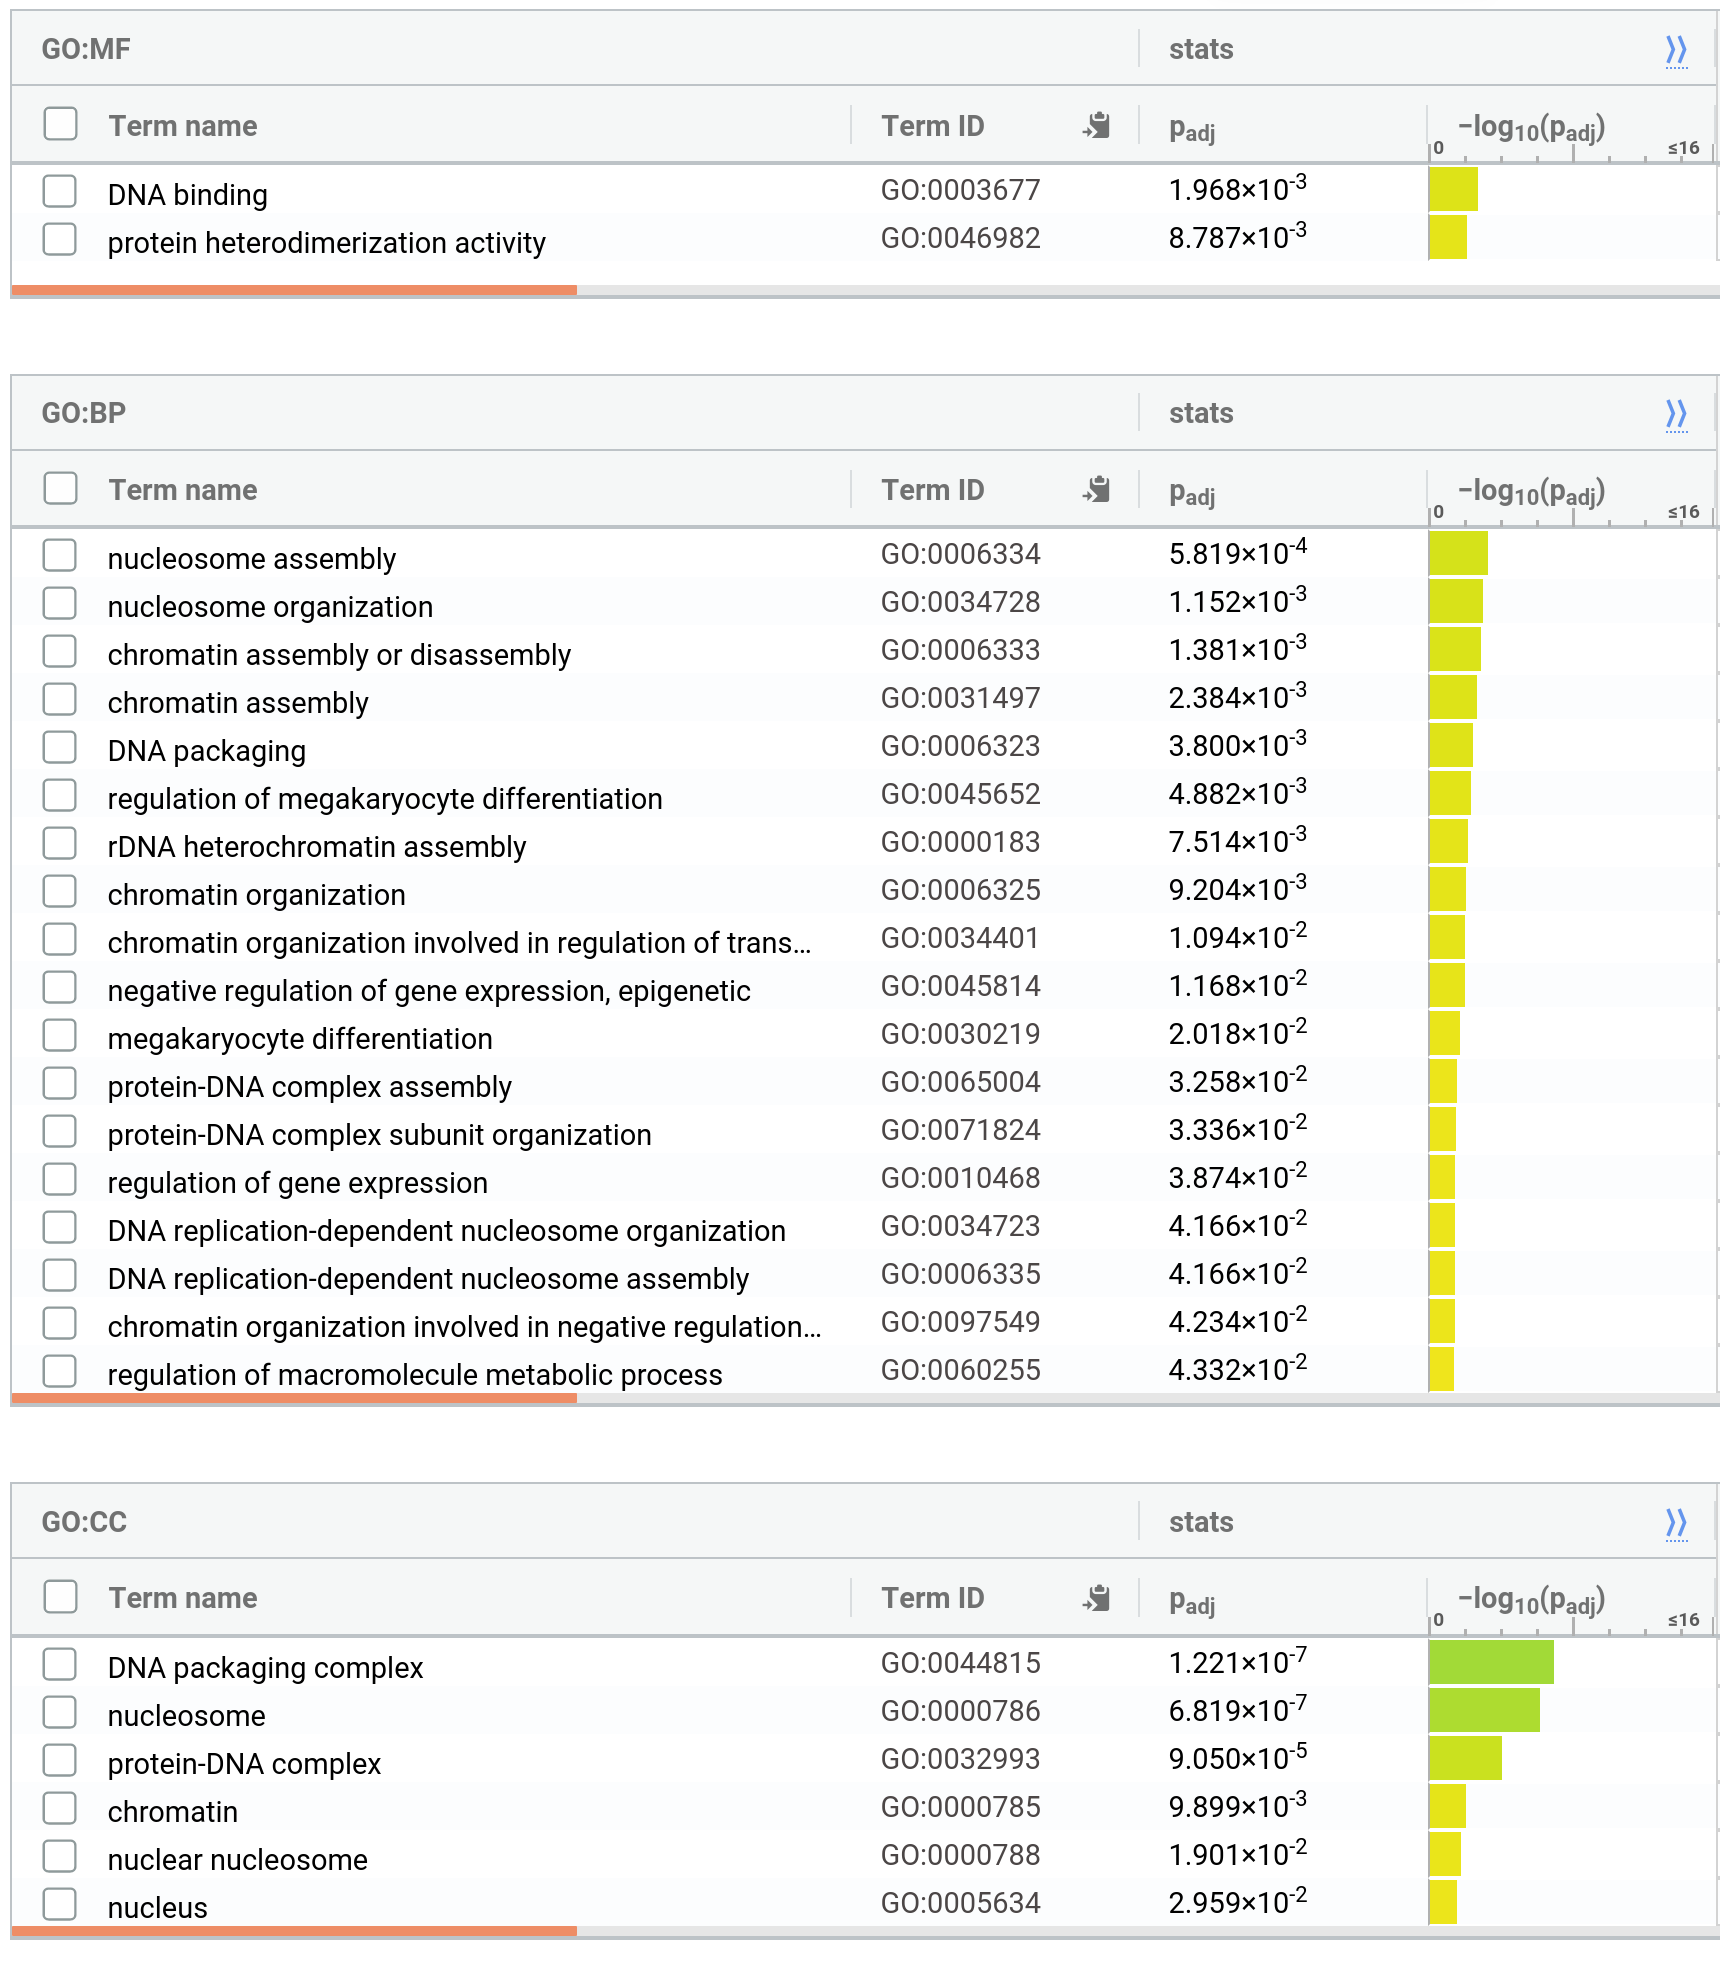
\includegraphics[width=\textwidth]{images/gprofiler/all_terms/ukbbint_all_terms.png}
    \caption{g:profiler GO enrichment results for significant genes found at GWGAS for the Intelligence\textsubscript{Discovery} sample}
    \label{fig:gprofiler intelligence discovery}
\end{figure}

\subsubsection{SynGO Intelligence Discovery}

No significant terms were enriched for cellular component. The terms enriched for biological process are in figure~\ref{tab:SynGO Enrichment UKBB intelligence significant genes. FDR}. Although the FDR values are higher than found in the Education\textsubscript{Discovery}, some synaptic terms are found to be enriched by using a limited ontology. 

\begin{table}[]
    \centering
    \begin{tabular}{llll}
    \toprule
      Term   & n & P & FDR q  \\
      \midrule
       synapse organization&	11&	$1.81\times10^{-4}$&	$1.81\times10^{-3}$\\
process in the synapse&	17&	3.01e-3&	0.0107\\
regulation of synapse organization&	3&	3.93e-3&	0.0107\\
modification of postsynaptic structure&	3	&4.29e-3	&0.0107\\
regulation of presynaptic membrane potential&	3&	9.62e-3&	0.0192  \\ 
\bottomrule
    \end{tabular}
    \caption{SynGO Enrichment Intelligence\textsubscript{Discovery} sample of genome wide significant genes at GWGAS. Correction for multiple comparisons using FDR. Background gene set is all brain expressed genes.}
    \label{tab:SynGO Enrichment UKBB intelligence significant genes. FDR}
\end{table}



% % latex table generated in R 3.6.3 by xtable 1.8-4 package
% % Sun Aug 30 16:17:46 2020
% \begin{table}[ht]
% \centering
% \begin{tabular}{llrrrrll}
%   \toprule
% GO ID& Description & Ref & Test & E & Fold & P & FDR \\ 
%   \midrule
%     GO:0000786 & nucleosome  & 77 & 8 & 0.7 & 11.11 & $1.23 \times 10^{-6}$ & 0.0012 \\ 
%   \hspace{2mm}\ding{213}  GO:0032993 & protein-DNA complex  & 175 & 9 & 1.6 & 5.50 & $5.67 \times 10^{-5}$ & 0.0095 \\ 
%  \hspace{2mm}\ding{213}  GO:0044815 & DNA packaging complex  & 85 & 9 & 0.8 & 11.32 & $2.26 \times 10^{-7}$ & 0.0005 \\ 

%   \hspace{2mm}\ding{213}   GO:0000785 & chromatin  & 1229 & 25 & 11.5 & 2.18 & $3.29 \times 10^{-4}$ & 0.0472 \\ 
%   \hspace{4mm}\ding{221}   GO:0043229 & intracellular organelle  & 12843 & 150 & 120.1 & 1.25 & $7.58 \times 10^{-6}$ & 0.0030 \\ 
%   \hspace{6mm}\ding{235}   GO:0005622 & intracellular  & 14693 & 165 & 137.4 & 1.20 & $5.80 \times 10^{-6}$ & 0.0039 \\ 
%   \hspace{6mm}\ding{235}  GO:0043226 & organelle  & 13859 & 157 & 129.6 & 1.21 & $2.35 \times 10^{-5}$ & 0.0059 \\ 
%   \hspace{8mm}\ding{233} GO:0110165 & cellular anatomical entity  & 18761 & 191 & 175.4 & 1.09 & $3.060 \times 10^{-5}$ & 0.0056 \\ 
   
   
%   GO:0031981 & nuclear lumen  & 4786 & 68 & 44.8 & 1.52 & $1.60 \times 10^{-4}$ & 0.0247 \\ 
%   \hspace{2mm}\ding{213} GO:0005634 & nucleus  & 7567 & 102 & 70.8 & 1.44 & $6.21 \times 10^{-6}$ & 0.0031 \\ 
%   \hspace{4mm}\ding{221} GO:0043231 & \makecell{intracellular membrane-bounded\\ organelle}  & 11028 & 134 & 103.1 & 1.30 & $9.470 \times 10^{-6}$ & 0.0032 \\ 
  
  
%   \hspace{6mm}\ding{235} GO:0043227 & membrane-bounded organelle  & 12734 & 148 & 119.1 & 1.24 & $1.620 \times 10^{-5}$ & 0.0046 \\ 
  
 
  
% %   GO:0005575 & cellular\_component  & 18946 & 192 & 177.2 & 1.08 & $2.420 \times 10^{-5}$ & 0.0054 \\ 
  
% %   UNCLASSIFIED & Unclassified  & 1905 & 3 & 17.8 & 0.17 & $2.420 \times 10^{-5}$ & 0.0049 \\ 
%   \bottomrule
% \end{tabular}
% \caption{Gene Ontology Enrichment in PANTHER using cellular component complete for significant genes at GWGAS for Intelligence\textsubscript{Discovery FDR} sample. Over represenation of terms only shown. Indendation shows depth of term in GO DAG, least indented deepest term.   Ref reference set, test:number of genes being tested present in ontology term E expected number of genes being tested present in ontology term, Fold= Fold changeP = raw p value, FDR = false discovery rate,} 
% \label{tab:GO cellular component complete Intelligence Discovery FDRover represenation only}
% \end{table}


% \begin{figure}
%     \centering
%     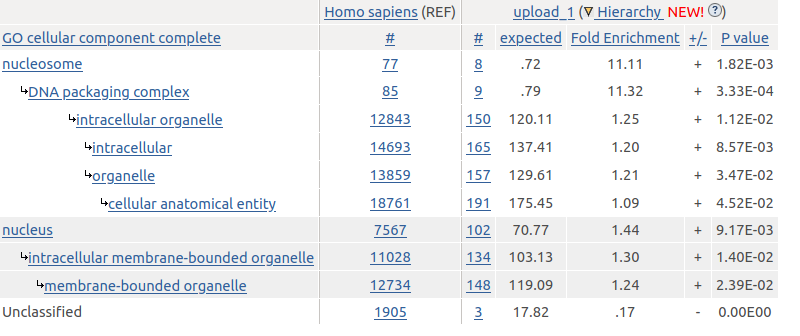
\includegraphics[width=\textwidth]{images/screenshots/ukbb_int_panther_cc_bonf.png}
%     \caption{UKBiobank intelligence significant genes at GWGAS. PANTHER GO enrichment Cellular component. Bonferroni correction. Screenshot for hierarchy}
%     \label{fig:UKBiobank significant genes at GWGAS. PANTHER GO enrichment Cellular component. Bonferroni correction. Screenshot for hierarchy}
% \end{figure}



% Previous to above did not match table
% \begin{figure}
%     \centering
%     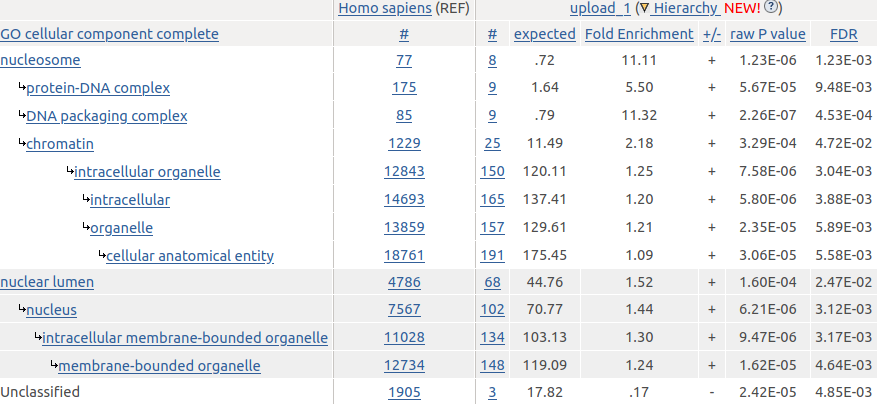
\includegraphics[width=\textwidth]{images/screenshots/ukbb_int_panther_cc_fdr.png}
%     \caption{UKBiobank intelligence significant genes at GWGAS. PANTHER GO enrichment Cellular component. FDR correction. Screenshot for hierarchy}
%     \label{fig:UKBiobank int significant genes at GWGAS. PANTHER GO enrichment Cellular component. FDR correction. Screenshot for hierarchy}
% \end{figure}


\paragraph{ToppGene}
 
Five biological processes terms, twenty nine molecular function terms and five cellular components had FDR $<$ 0.05. See figure~\ref{fig:toppgene pic}. The enrichment is that is present is also predominantly terms such as nucleosome function, DNA packaging and chromatin binding. Synaptic terms and neurogenesis terms are absent compared with the education samples.\footnote{int discovery PSP as BGNo GOBeta catenin pathway} 

\begin{figure}
    \centering
    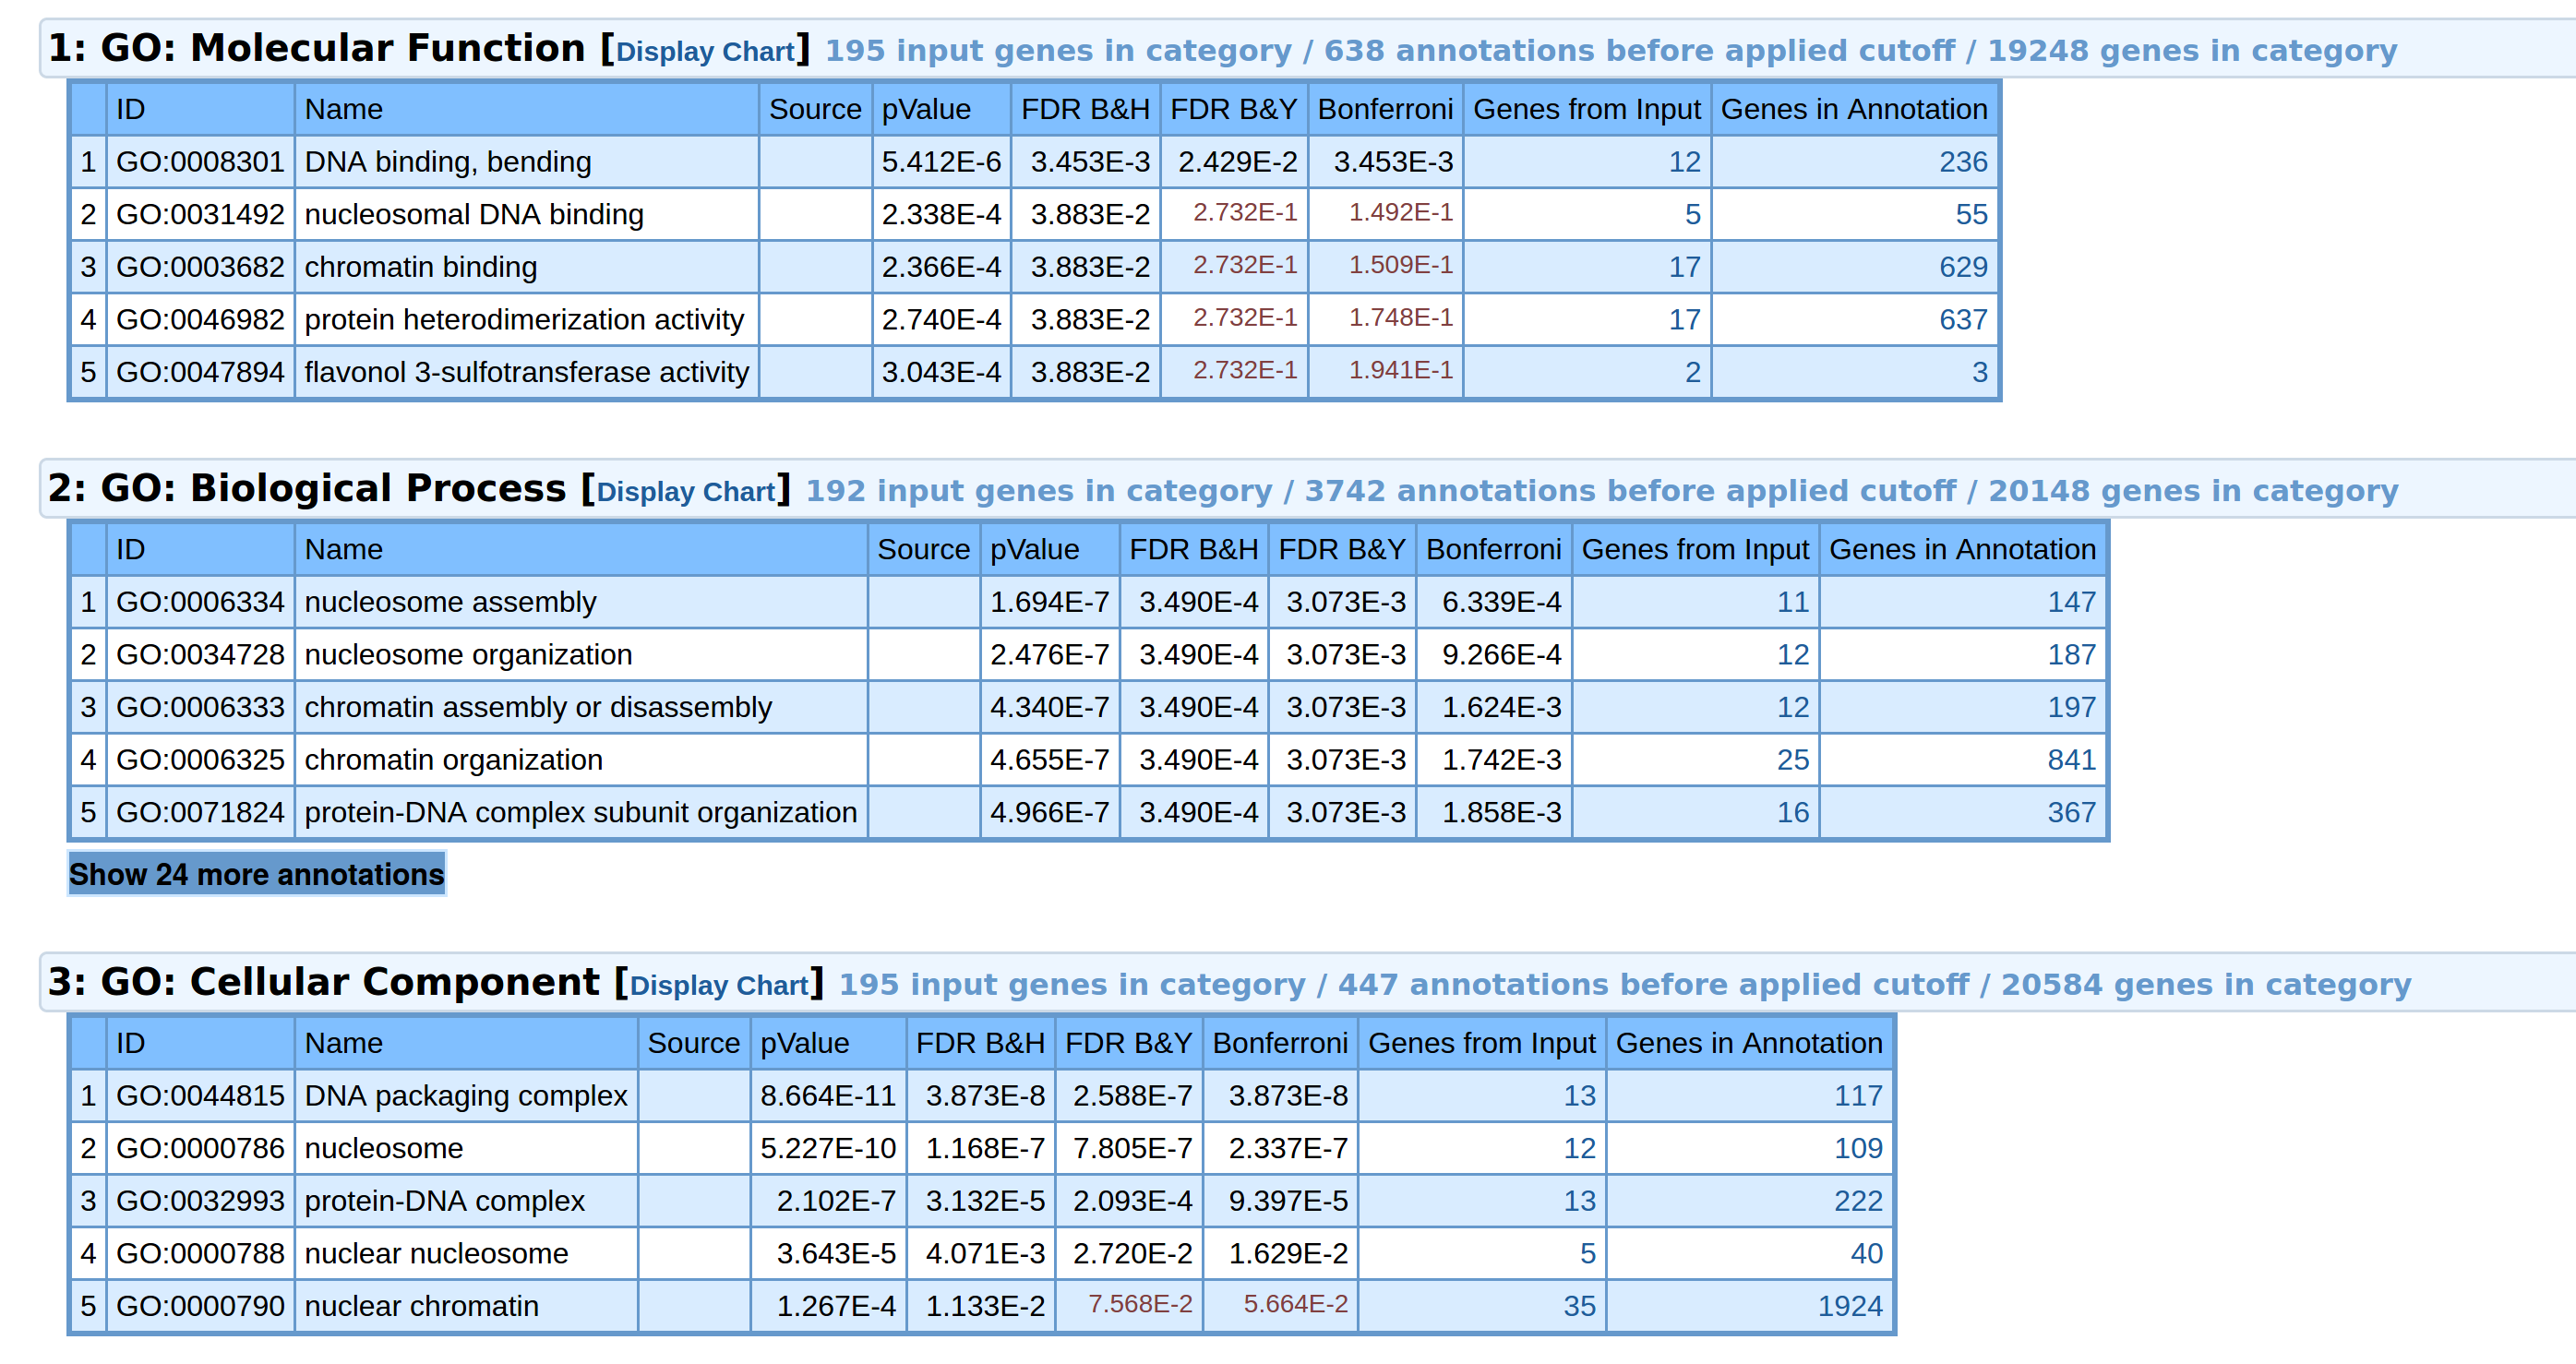
\includegraphics[width=\textwidth]{images/chapter2/strontium/images_toppgene_all_groups.png}
    \caption{Gene ontology ToppGene Biological Process, Molecular Function and Cellular component}
    \label{fig:toppgene pic}
\end{figure}



%\todo{use bg PSP}


% \todo[inline]{Important note to self, although there are other results they are not going to change the overall analysis therefore do not add any more just get this chapter done. If they are ready (ie formatted) and add to the PhD after completing the discussion they can be added. Potential data commented out in tex below}


There is no enrichment for genes differentially enriched in the central nervous system areas using GTEx version 8 analysed using FUMA (figure~\ref{fig:FUMA gtex deg samples multiple} and fig~\ref{fig:deg_upref_sample_gtex_gener}).

% Removed 20th Sep as now appears in multiple view
% \begin{figure}        
%     \centering
%     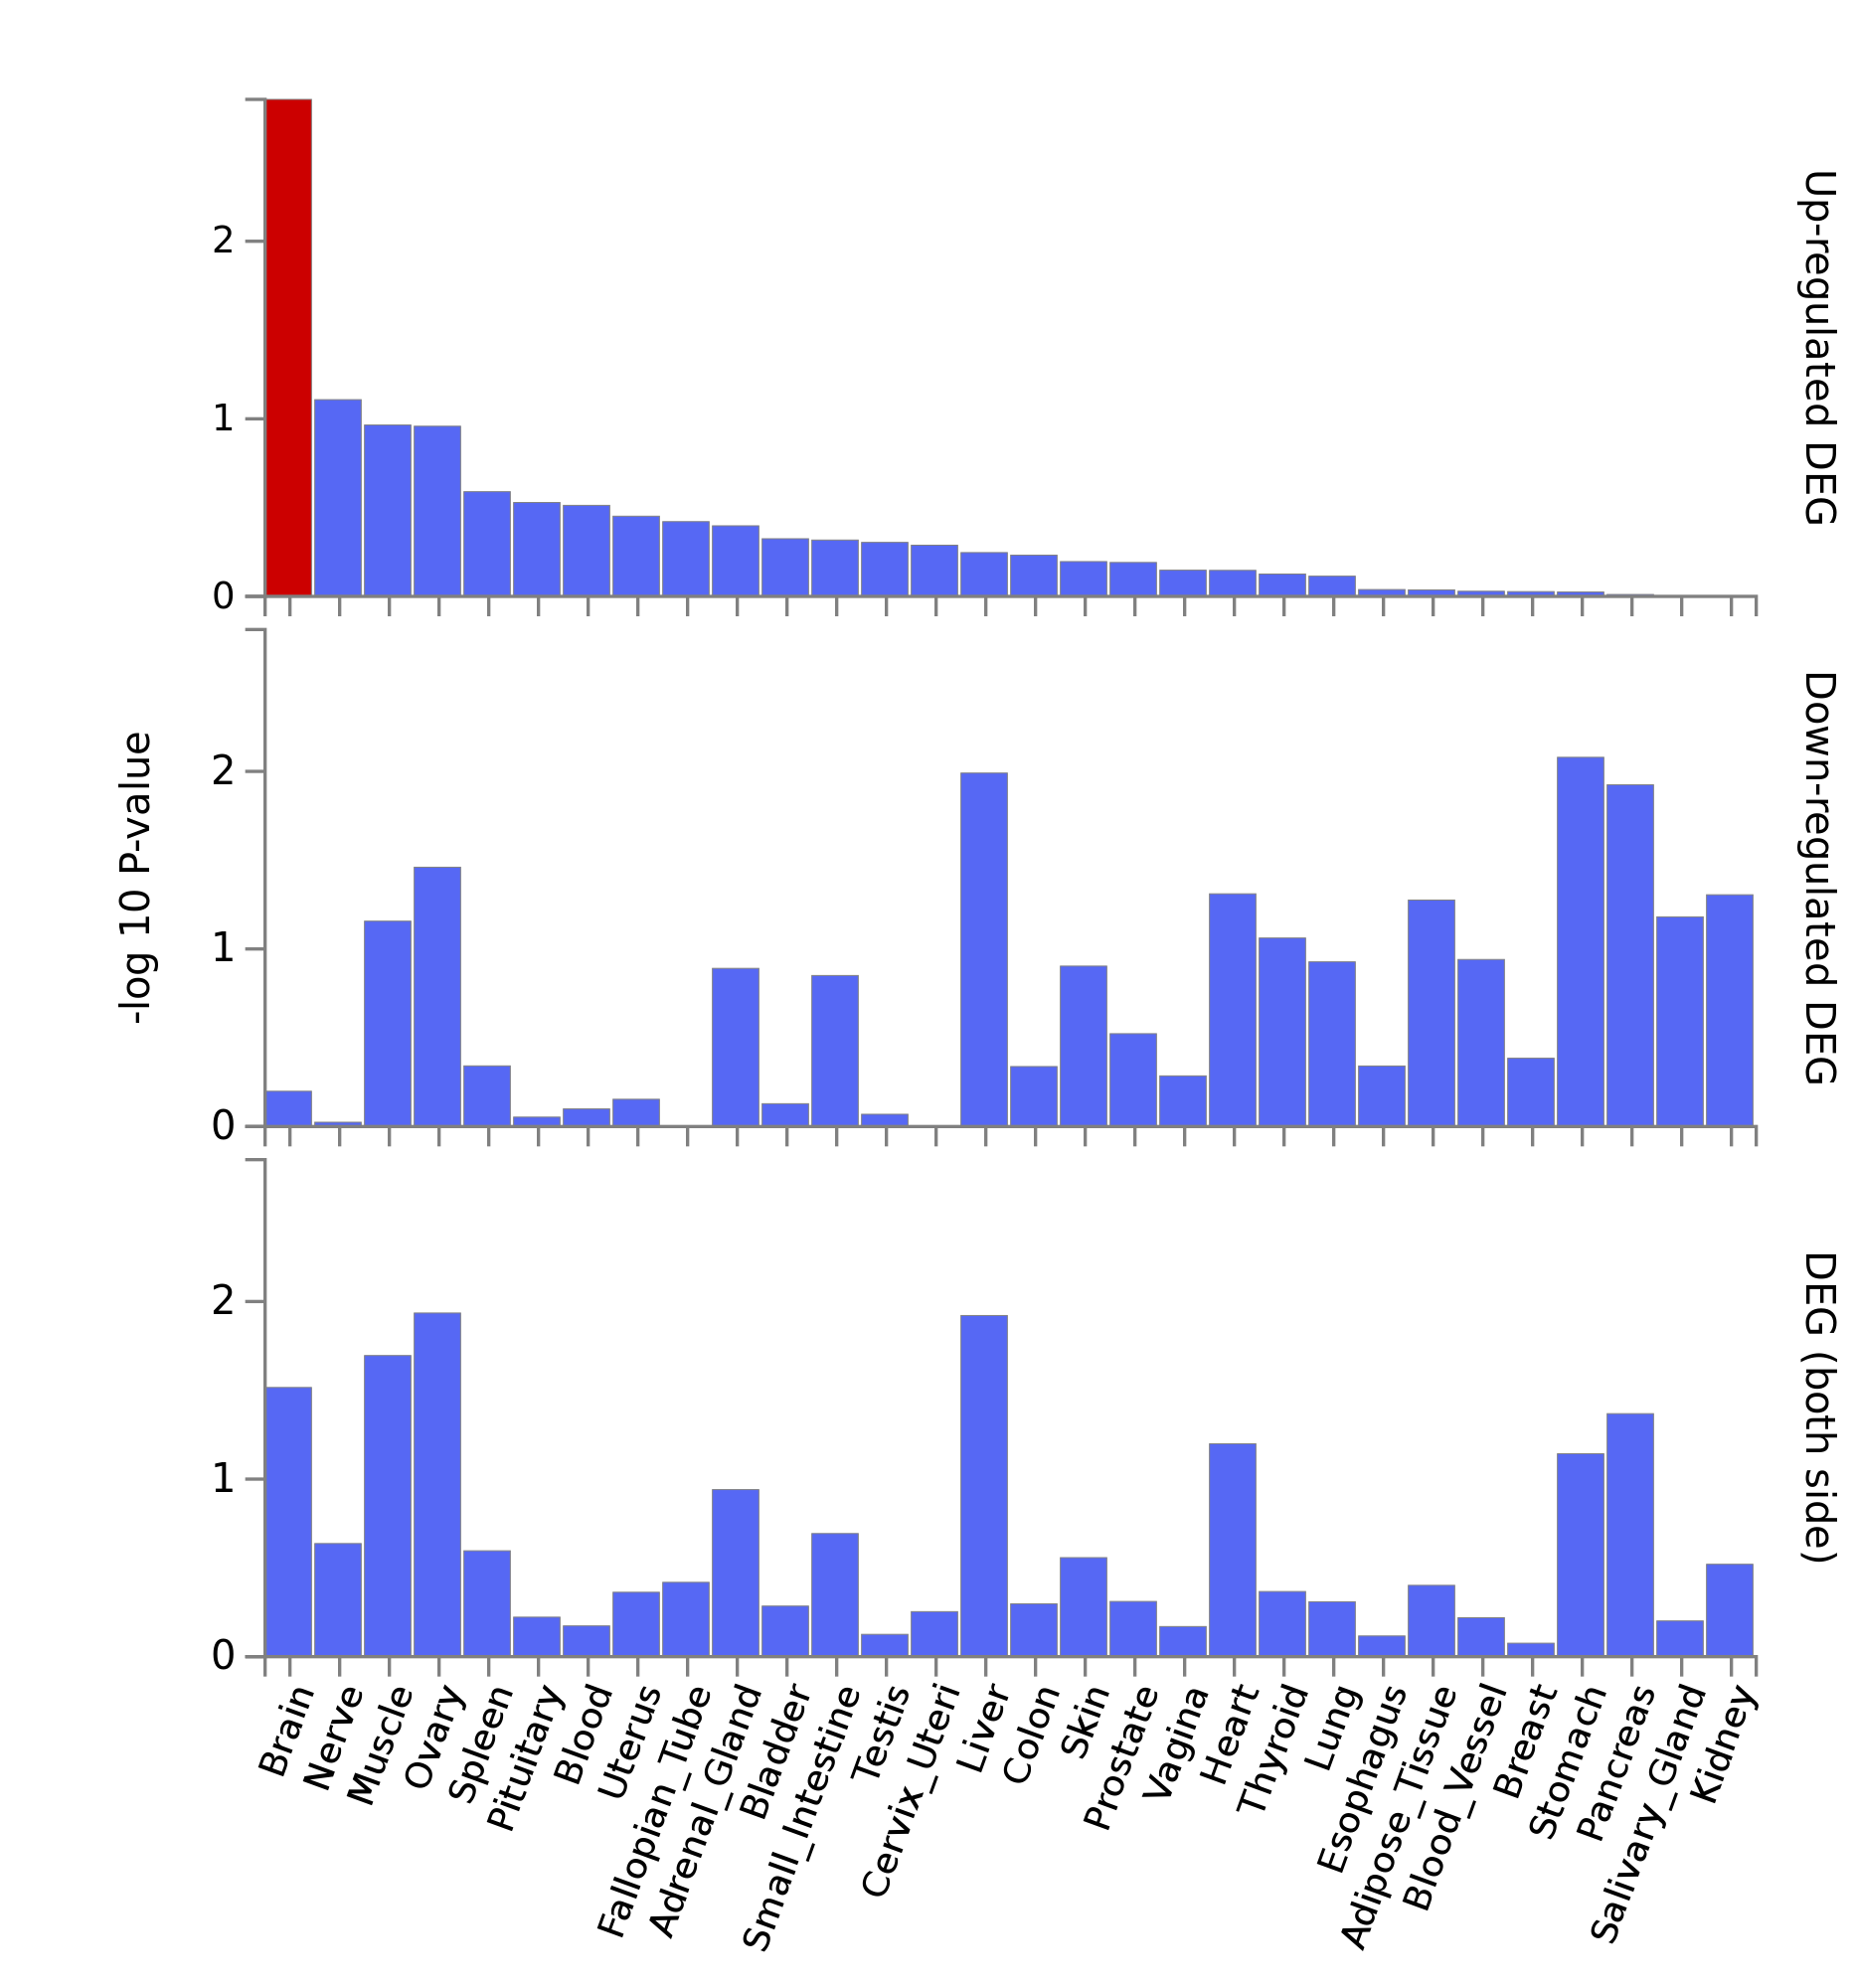
\includegraphics[width=\textwidth]{images/FUMA_plots/gtex_30_ukbbed.png}
%     \caption{GTEx FUMA UKBBEd}
%     \label{fig:GTEx FUMA UKBBEd}
% \end{figure}




% \begin{figure}
%     \centering
%     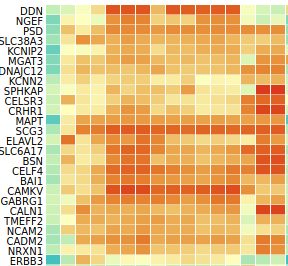
\includegraphics[width=\textwidth]{images/FUMA_plots/closeupdeg_ukbbed.png}
%     \caption{Caption}
%     \label{fig:my_label}
% \end{figure}
% \subsection{Education\textsubscript{Discovery} Ontology enrichment}

% \subsection{Intelligence Discovery}
% 197 genes
% 11 missing using ENSG annotations


% Gene ID 3 unmappedZZ
% GeneID:100132074 FOXO6
% GeneID:9753
% GeneID:3107

% Symbol
% MGEA5
% C10orf76
% CCDC101 SGF29
% PET112 GATB
% HIST1H3C H3C3 one of 25 synonyms
% HIST1H3I HIST1H3J one of 24 synonyms
% BAI1 ADGRB1
% RP5-874C20.3 pseudogene entrz 7741 ZSCAN26

% REMAINING FRAMEWORK BELOW
%     \subsection{Intelligence Discovery}
%         \subsubsection{Authors findings Intelligence Discovery}
% %         \todo[inline]{by Hill et all ? move to samples. Points to make big gene sets}
% Gene set analysis of this set augmented by mgtag \cite{hill2019combined} was carried out using 10891 gene sets from Gene ontology, Reactome and MSigDB (raw p required = 0.05/10891 = $4.59 \times 10^{-6}$. GSA revealed 7 sets including neurogenesis 1355 genes and genes expressed in synapse 717 genes , regulation of nervous system development 722 genes neuron projection 989 neuron differentation 842 and CNS neuron differentiation 160 genes cell development 808 genes (\textcolor{red}{quote p or do table})

% For gene set size analysis see\footnote{\url{source('~/RProjects/paper_xls_output/R/exploratory_data_analysis/gene_size_and_enrichment_magma_sets.R')}} table~\ref{tab:group size and enrichment}

%         \subsubsection{Ontology ORA Genome Intelligence discovery}
%         196 genes 
%         \paragraph{panther Intelligence discovery}3 unmapped GeneID:100132074
% GeneID:9753
% GeneID:3107
% \subparagraph{panther BP all Intelligence Discovery} Nil
% \subparagraph{panther MF all Intelligence Discovery}DNA binding 	2486 	44 	22.53 	1.95 	+ 	1.40E-05 	1.66E-02
% nucleic acid binding 	4024 	60 	36.47 	1.64 	+ 	5.93E-05 	4.70E-02
% binding 	16464 	171 	149.23 	1.15 	+ 	4.44E-05 	4.23E-02
% protein binding 	14110 	156 	127.90 	1.22 	+ 	6.81E-06 	1.08E-02
% \begin{figure}
%     \centering
%     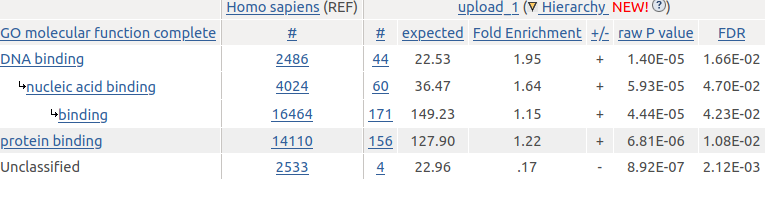
\includegraphics[width=\textwidth]{images/screenshots/GO_MF_Panther_UKBBInt_Heirarchy.png}
%     \caption{Panther MF UKBB Intelligence}
%     \label{fig:panther mf ukbb intelligence}
% \end{figure}
% \subparagraph{panther CC all Intelligence Discovery}
% \begin{figure}
%     \centering
%     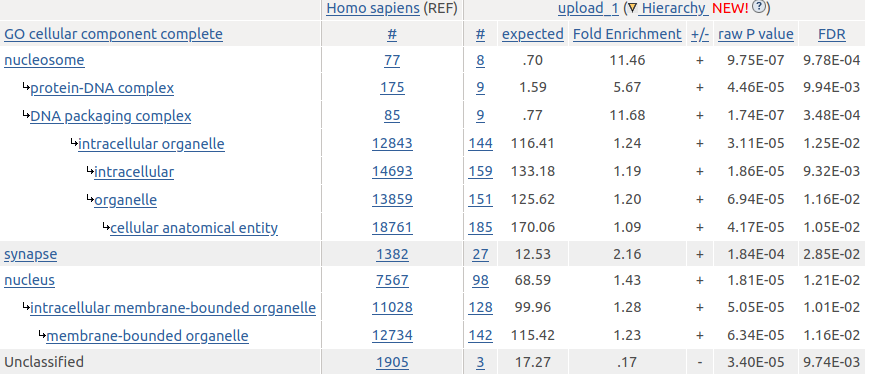
\includegraphics[width=\textwidth]{images/screenshots/panther_cc_ukbb_int_all.png}
%     \caption{Panther hierarchy cc ukbb int all}
%     \label{fig:panther hierarchy cc ukbb int all}
% \end{figure}
%          \subsubsection{Ontology ORA Synaptic}
%          \subsubsection{Others}
%         Path to code
        
%         GTEx
   

\subsection{Education Discovery Ontology Over representation analysis}
      The 235 genome-wide significant genes identified using MAGMA GWGAS for the Education\textsubscript{Discovery} sample (section~\ref{sec:UKBB Education discovery GWGAS}) were tested for over-representation of ontology terms. 
      Using PANTHER, I was unable to have all of the significant genes output by MAGMA identified, and used the gene identifier with the most uniquely identified genes  (233 terms, HGNC symbols with synonyms\footnote{ Script at \url{source('~/RProjects/paper_xls_output/R/chapter_2/FUMA/edit_gene_table/UKBB_Ed_FUMA2clipboard.R')}}).\footnote{entrez 231, hgnc (symbol) 225, NCBI symbol 227, HGNC ID 232 for HGNC id see \url{source('~/RProjects/paper_xls_output/R/chapter_2/translate_sig_genes/ukbbed_NCBI_translate2.R')})}.
        
    Thirty-three biological process ontology terms, were over-represented (FDR corrected $q<$0.05) amongst the 233 significant genes (see figure~\ref{fig:panther bp ukbb edu fdr}). There are several enriched terms related to neurogenesis and axonal development, similar to the Education\textsubscript{Replication} sample but distinct from the Intelligence samples. The most significant term (FDR=$8.51\times10^{-4}$) was ``nervous system development" (GO:0007399, 57 genes found amongst 2432 in the annotation). Many of the sets are broad and non-specific; the lowest FDR for annotations with less than 500 genes was ``negative regulation of cell projection" (GO:0031345);11 of 183 genes;5.4 fold change; FDR=0.0089.  Considering only those terms with greater than mean fold change (2.61), the most enriched is ``regulation of nervous system development" (GO:0051960,FDR 0.003). There was no significant over-representation of molecular function terms. 
    
    \begin{figure}
                \centering
                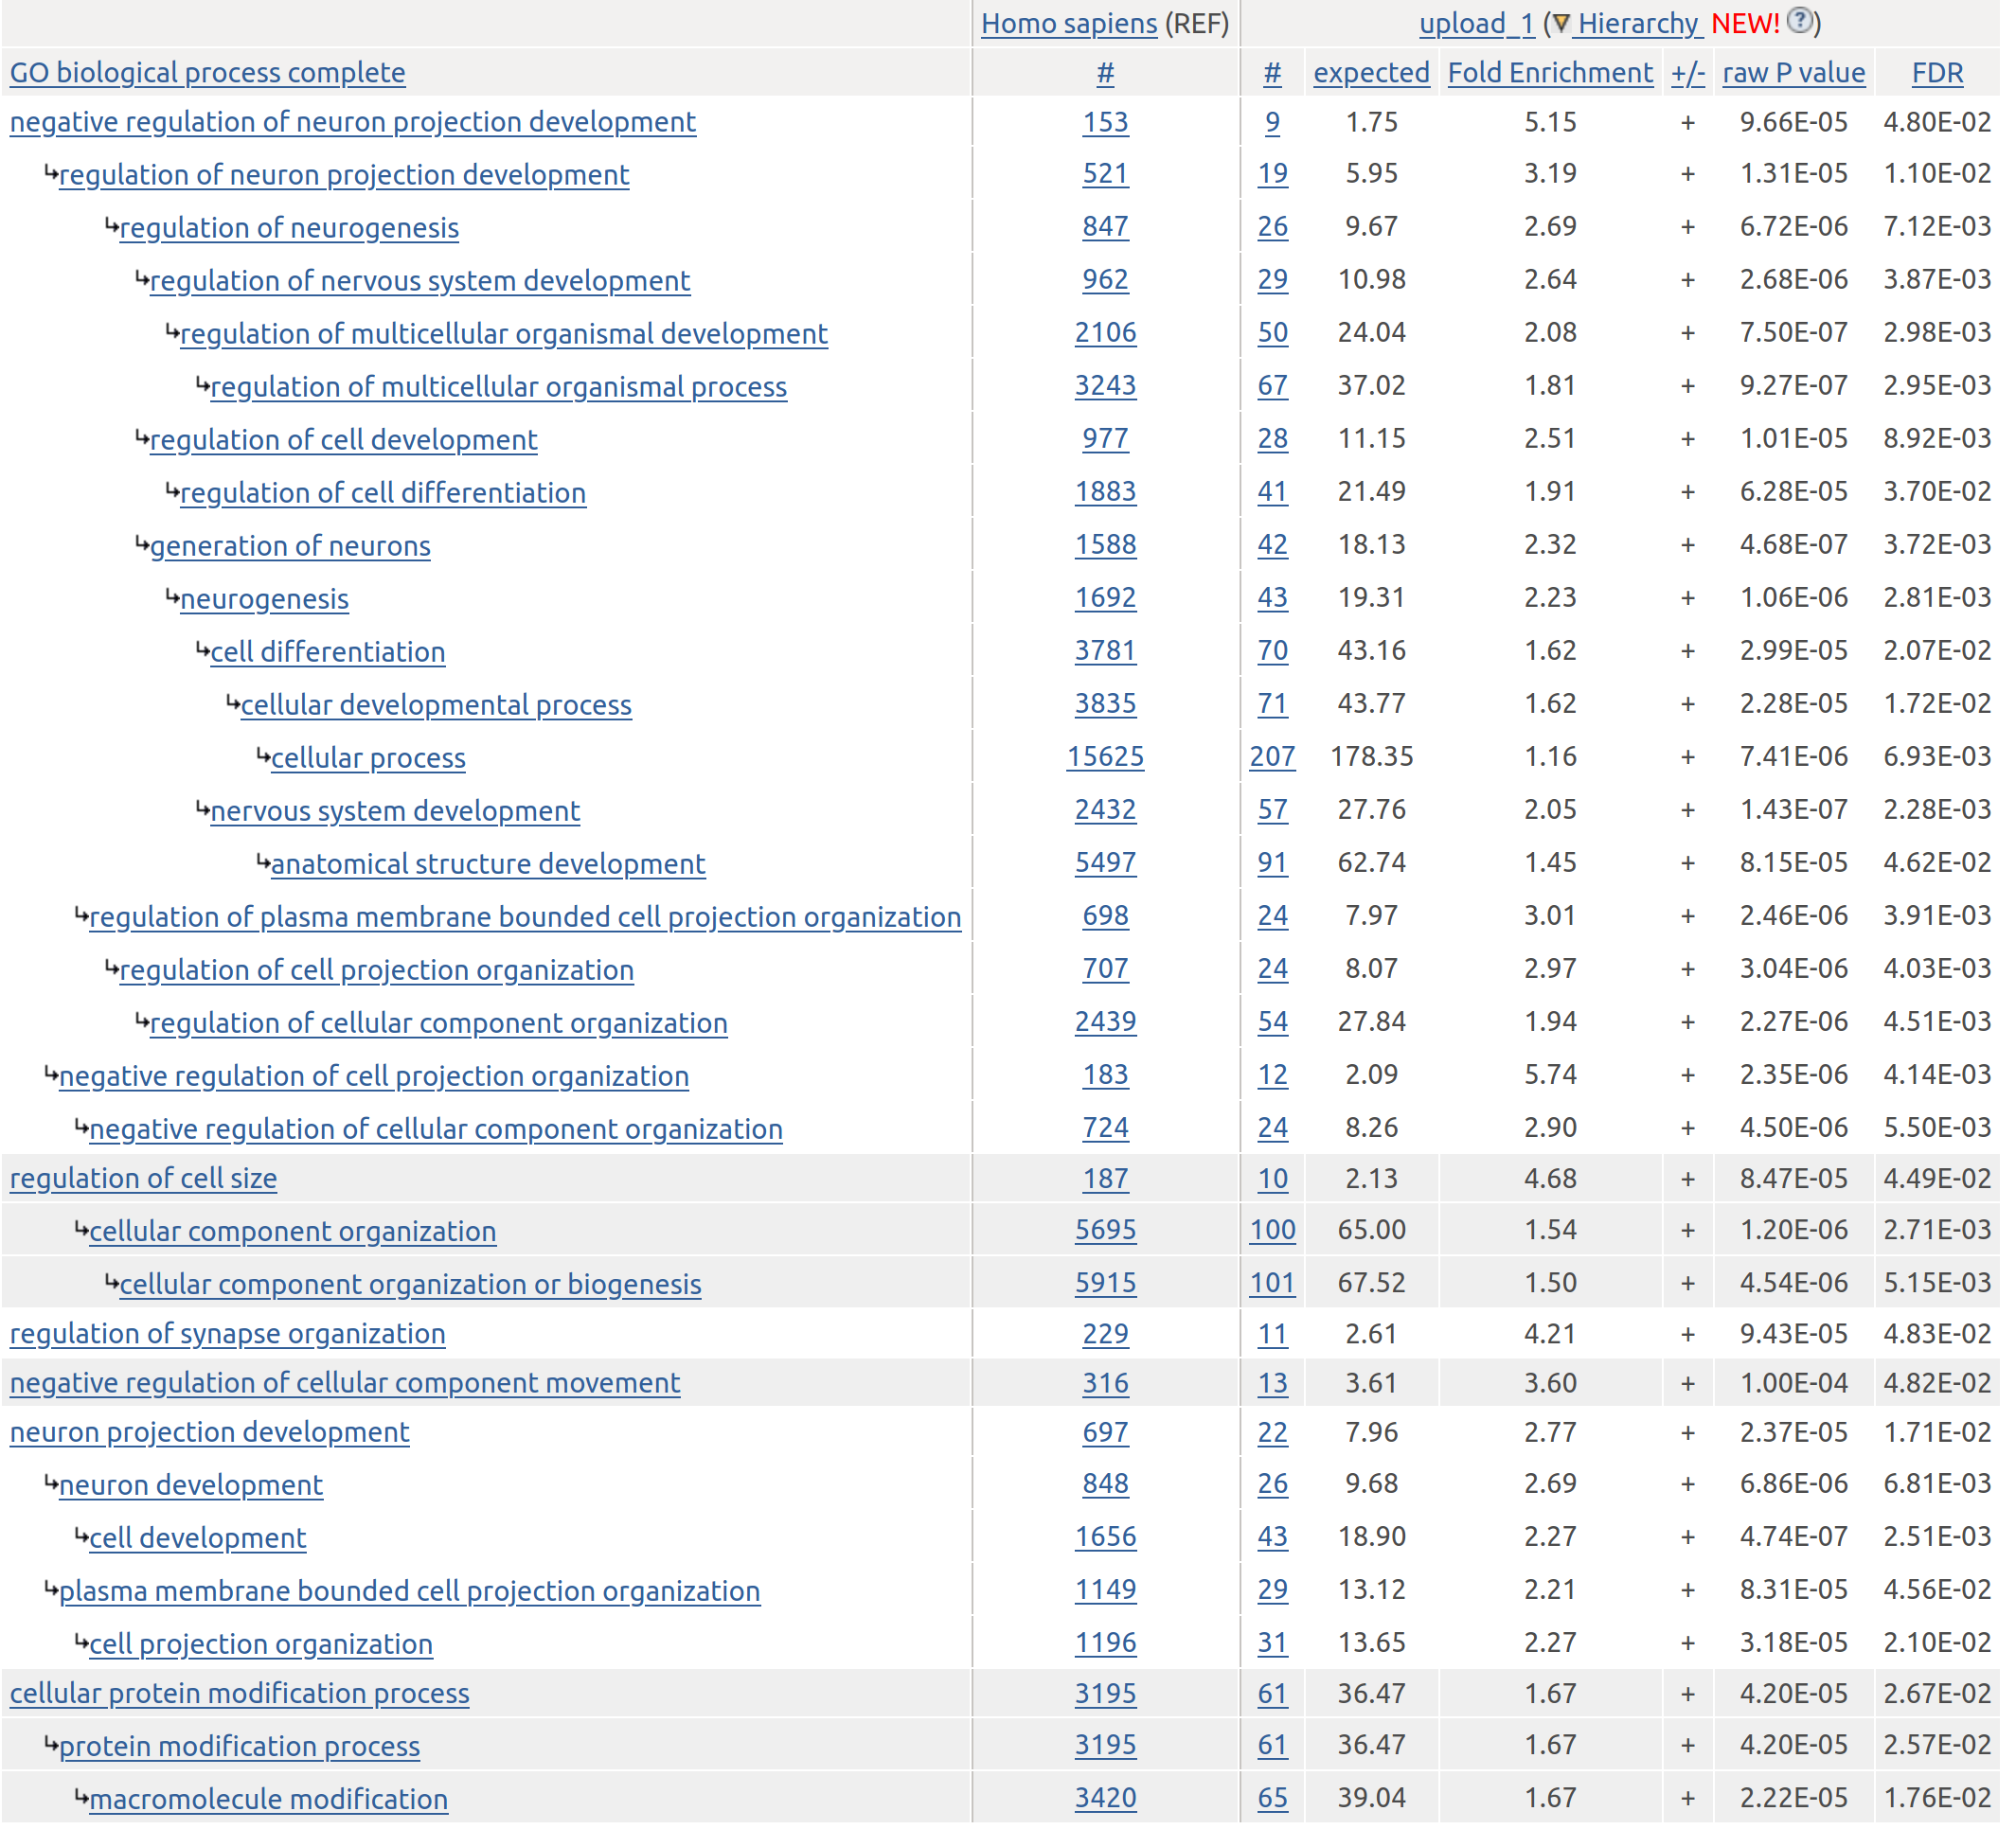
\includegraphics[width=\textwidth]{images/chapter2/large_screenshots/edu_discovery_bp_allbg_panther.png}
                \caption{PANTHER Gene Ontology Enrichment Biological Process Education\textsubscript{Discovery} FDR Large}
                \label{fig:panther bp ukbb edu fdr}
            \end{figure}
            
            
    Forty cellular component terms were over-represented.  Five of the ten most enriched terms had over 10,000 genes in their annotation. This includes the most significant term ``Intracellular" (GO:0005622, 14707 genes, FDR=$4.9\times10^{-5}$) although only six of the forty significant terms contained over 10,000 genes (see figure~\ref{fig:panther cc ukbb edu } and table \label{tab:GO cellular component complete Education Discovery FDRover represenation only}). Four terms have under 100 annotations amongst the ten most enriched, three are related to the endoplasmic reticulum  including  ``lumenal side of membrane" (GO:0098576 FDR =   $3.84\times10^{-4}$)), one is annotated to GO:0042613 ``MHC class II protein complex" ;(5 of 19 genes in annotation found;  fold change 23.1, FDR=0.00126).``Synapse" ( GO:0045202  ;   36 of 1383genes in annotation,    ; fold change 15.8,  FDR= 0.00116) was also amongst the ten most enriched terms.    \footnote{ GABAergic synapse is present as an enriched cellular component term GO:0098982 79 in annotation 6 terms FDR=0.0253 but the genes DAG1, Dystroglycan;Neurexin-1, NRXN1 ;SLC6A17,Sodium-dependent neutral amino acid transporter; PCDH17,Protocadherin-17;ERBB4,Receptor tyrosine-protein kinase erbB-4;BSN,Protein Bassoon.} No SLIM ontologies showed significant over-representation and there was no enrichment of PANTHER pathways. Only the protein class PC00149 ``major histocompatibility complex protein" was over-represented  *5 of 18 terms; 24.3 fold change; FDR=0.0010).

            

            % \subparagraph{CC Panther Education Discovery}
            % 40 terms. Of the 10 terms with the lowest FDR 5 have more than 10000 genes in the annotation (Lowest FDR: GO:0005622 intracellular 14704 genes in annotation FDR=$4.9\times10^{-5}$, 2nd GO:0043231 intracellular membrane-bounded organelle                              11041 in annotation  166 Genes from significant genes annotated, 4th GO:0043229 intracellular organelle                                               12856 in annotation , 183 in significant genes; 5th Organelle GO:0043226 organelle                                                             13868 in annotation,  193 in test genes and 8thGO:0043227 membrane-bounded organelle                                            12748  in annotation. 4 terms have under 100 annotations in the top 10, 3 are related to the endoplasmic reticulum (top GO:0098576 lumenal side of membrane                                             ;in annotation    37 genes, number of significant genes     7;  fold change 16.6,  FDR =   $3.84\times10^{-4}$), one is annotated to GO:0042613 MHC class II protein complex                                     , ;genes in annotation        19, significant genes with annotation     5;  fold change 23.1, FDR=0.00126. The final top 10 cellular component annotation is  GO:0045202 synapse                                                            ;    1383genes in annotation,    36 significant genes with annotation; fold change 15.8,  FDR= 0.00116. Post synapse is also enriched 22 significant genesw in 651 in annotation, fold change 2.96, FDR=0.00157.
            % See figure~\ref{fig:panther cc ukbb edu } for results displayed with terms sorted to show their position in the hierarchy.
            
       
            
            \begin{figure}
                \centering
                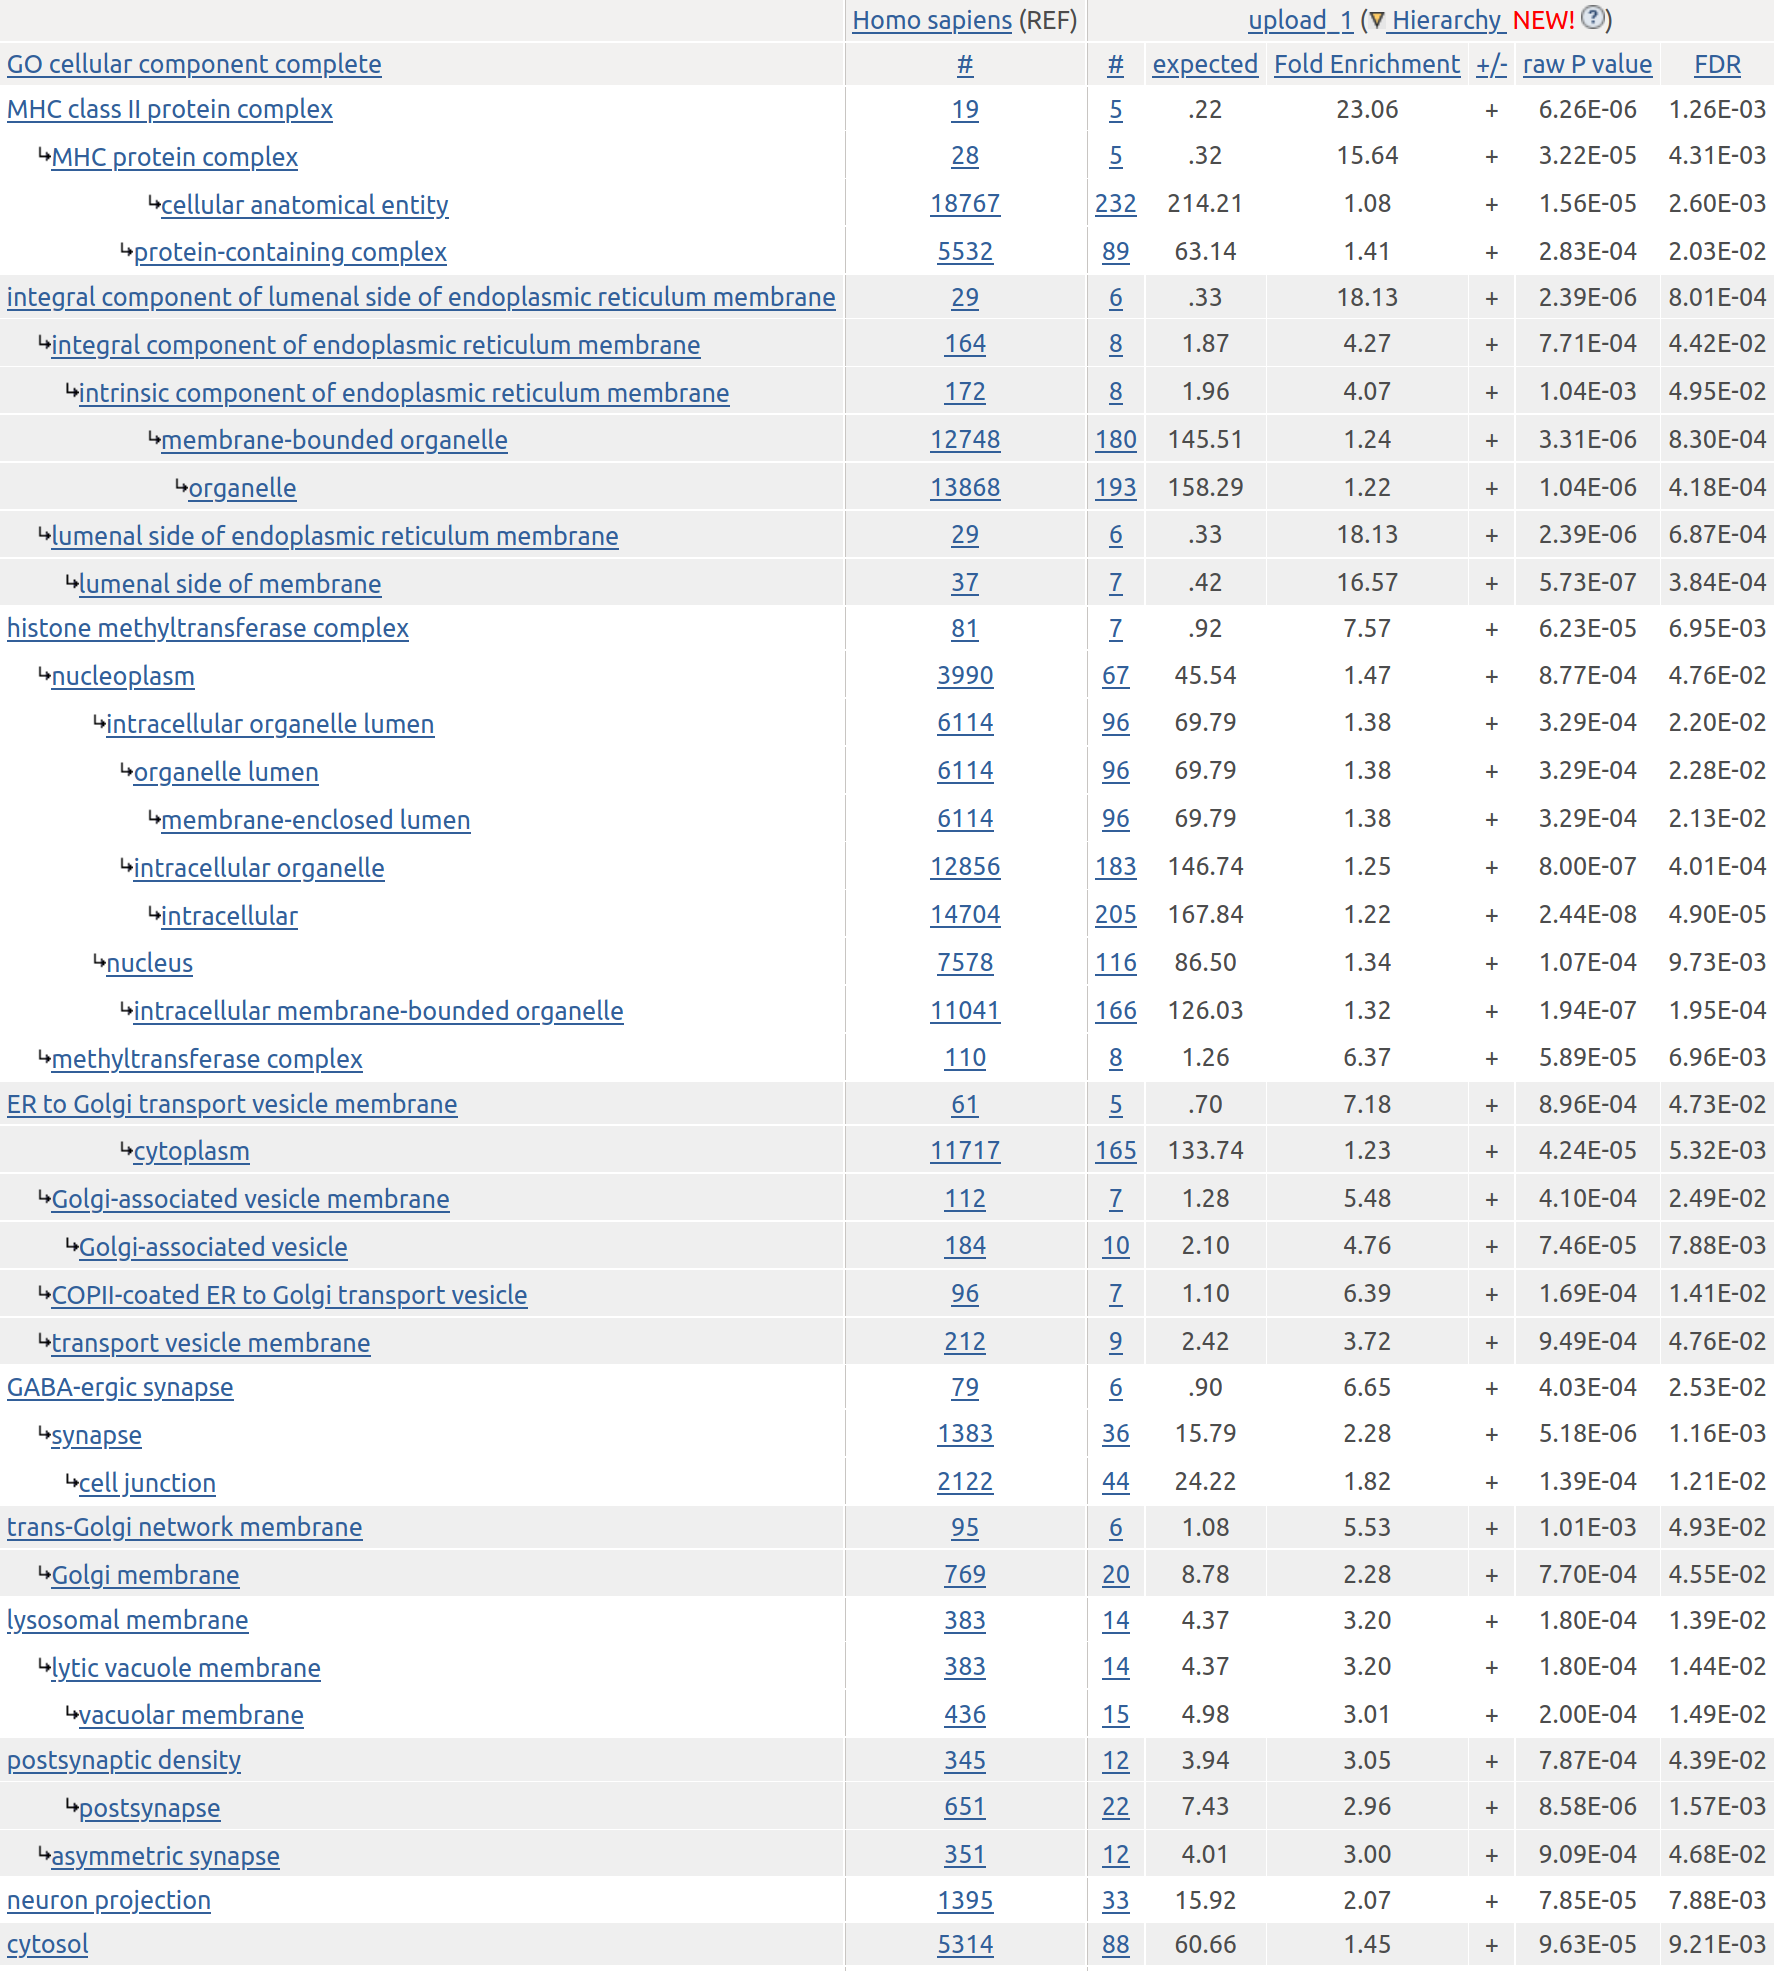
\includegraphics[width=\textwidth]{images/chapter2/large_screenshots/edu_discovery_large_cc_panther.png}
                \caption{PANTHER Gene Ontology Enrichment Cellular Component Education\textsubscript{Discovery}. The lowest FDR again is found in the most general and largest gene ontology terms with correspondingly small fold enrichment. }
                \label{fig:panther cc ukbb edu }
            \end{figure}
            
            
\begin{table}[ht]
\centering
\begin{adjustbox}{width=\textwidth}

\begin{tabular}{llrrrrrr}
  \hline
GO & description & Ref & Test & E & Fold & P & FDR \\ 
  \hline
GO:0042613 & MHC class II protein complex  & 19 & 5 & 0.2 & 23.06 & $6.26 \times 10^{-6}$ & 0.0013 \\ 
  GO:0071556 & integral component of lumenal side of endoplasmic reticulum membrane  & 29 & 6 & 0.3 & 18.13 & $2.39 \times 10^{-6}$ & 0.0008 \\ 
  GO:0098553 & lumenal side of endoplasmic reticulum membrane  & 29 & 6 & 0.3 & 18.13 & $2.39 \times 10^{-6}$ & 0.0007 \\ 
  GO:0098576 & lumenal side of membrane  & 37 & 7 & 0.4 & 16.57 & $5.73 \times 10^{-7}$ & 0.0004 \\ 
  GO:0042611 & MHC protein complex  & 28 & 5 & 0.3 & 15.64 & $3.22 \times 10^{-5}$ & 0.0043 \\ 
  GO:0035097 & histone methyltransferase complex  & 81 & 7 & 0.9 & 7.57 & $6.23 \times 10^{-5}$ & 0.0069 \\ 
  GO:0012507 & ER to Golgi transport vesicle membrane  & 61 & 5 & 0.7 & 7.18 & $8.96 \times 10^{-4}$ & 0.0473 \\ 
  GO:0098982 & GABA-ergic synapse  & 79 & 6 & 0.9 & 6.65 & $4.03 \times 10^{-4}$ & 0.0253 \\ 
  GO:0030134 & COPII-coated ER to Golgi transport vesicle  & 96 & 7 & 1.1 & 6.39 & $1.69 \times 10^{-4}$ & 0.0141 \\ 
  GO:0034708 & methyltransferase complex  & 110 & 8 & 1.3 & 6.37 & $5.89 \times 10^{-5}$ & 0.0070 \\ 
  GO:0032588 & trans-Golgi network membrane  & 95 & 6 & 1.1 & 5.53 & $1.01 \times 10^{-3}$ & 0.0493 \\ 
  GO:0030660 & Golgi-associated vesicle membrane  & 112 & 7 & 1.3 & 5.48 & $4.10 \times 10^{-4}$ & 0.0249 \\ 
  GO:0005798 & Golgi-associated vesicle  & 184 & 10 & 2.1 & 4.76 & $7.46 \times 10^{-5}$ & 0.0079 \\ 
  GO:0030176 & integral component of endoplasmic reticulum membrane  & 164 & 8 & 1.9 & 4.27 & $7.71 \times 10^{-4}$ & 0.0442 \\ 
  GO:0031227 & intrinsic component of endoplasmic reticulum membrane  & 172 & 8 & 2.0 & 4.07 & $1.04 \times 10^{-3}$ & 0.0495 \\ 
  GO:0030658 & transport vesicle membrane  & 212 & 9 & 2.4 & 3.72 & $9.49 \times 10^{-4}$ & 0.0476 \\ 
  GO:0098852 & lytic vacuole membrane  & 383 & 14 & 4.4 & 3.20 & $1.80 \times 10^{-4}$ & 0.0144 \\ 
  GO:0005765 & lysosomal membrane  & 383 & 14 & 4.4 & 3.20 & $1.80 \times 10^{-4}$ & 0.0139 \\ 
  GO:0014069 & postsynaptic density  & 345 & 12 & 3.9 & 3.05 & $7.87 \times 10^{-4}$ & 0.0439 \\ 
  GO:0005774 & vacuolar membrane  & 436 & 15 & 5.0 & 3.01 & $2.00 \times 10^{-4}$ & 0.0149 \\ 
  GO:0032279 & asymmetric synapse  & 351 & 12 & 4.0 & 3.00 & $9.09 \times 10^{-4}$ & 0.0468 \\ 
  GO:0098794 & postsynapse  & 651 & 22 & 7.4 & 2.96 & $8.58 \times 10^{-6}$ & 0.0016 \\ 
  GO:0045202 & synapse  & 1383 & 36 & 15.8 & 2.28 & $5.18 \times 10^{-6}$ & 0.0012 \\ 
  GO:0000139 & Golgi membrane  & 769 & 20 & 8.8 & 2.28 & $7.70 \times 10^{-4}$ & 0.0455 \\ 
  GO:0043005 & neuron projection  & 1395 & 33 & 15.9 & 2.07 & $7.85 \times 10^{-5}$ & 0.0079 \\ 
  GO:0030054 & cell junction  & 2122 & 44 & 24.2 & 1.82 & $1.39 \times 10^{-4}$ & 0.0121 \\ 
  GO:0005654 & nucleoplasm  & 3990 & 67 & 45.5 & 1.47 & $8.77 \times 10^{-4}$ & 0.0476 \\ 
  GO:0005829 & cytosol  & 5314 & 88 & 60.7 & 1.45 & $9.63 \times 10^{-5}$ & 0.0092 \\ 
  GO:0032991 & protein-containing complex  & 5532 & 89 & 63.1 & 1.41 & $2.83 \times 10^{-4}$ & 0.0203 \\ 
  GO:0043233 & organelle lumen  & 6114 & 96 & 69.8 & 1.38 & $3.29 \times 10^{-4}$ & 0.0228 \\ 
  GO:0070013 & intracellular organelle lumen  & 6114 & 96 & 69.8 & 1.38 & $3.29 \times 10^{-4}$ & 0.0220 \\ 
  GO:0031974 & membrane-enclosed lumen  & 6114 & 96 & 69.8 & 1.38 & $3.29 \times 10^{-4}$ & 0.0213 \\ 
  GO:0005634 & nucleus  & 7578 & 116 & 86.5 & 1.34 & $1.07 \times 10^{-4}$ & 0.0097 \\ 
  GO:0043231 & intracellular membrane-bounded organelle  & 11041 & 166 & 126.0 & 1.32 & $1.94 \times 10^{-7}$ & 0.0002 \\ 
  GO:0043229 & intracellular organelle  & 12856 & 183 & 146.7 & 1.25 & $8.00 \times 10^{-7}$ & 0.0004 \\ 
  GO:0043227 & membrane-bounded organelle  & 12748 & 180 & 145.5 & 1.24 & $3.31 \times 10^{-6}$ & 0.0008 \\ 
  GO:0005737 & cytoplasm  & 11717 & 165 & 133.7 & 1.23 & $4.24 \times 10^{-5}$ & 0.0053 \\ 
  GO:0005622 & intracellular  & 14704 & 205 & 167.8 & 1.22 & $2.44 \times 10^{-8}$ & 0.0000 \\ 
  GO:0043226 & organelle  & 13  868 & 193 & 158.3 & 1.22 & $1.04 \times 10^{-6}$ & 0.0004 \\ 
%   GO:0110165 & cellular anatomical entity  & 18767 & 232 & 214.2 & 1.08 & $1.56 \times 10^{-5}$ & 0.0026 \\ 
%   GO:0005575 & cellular\_component  & 18951 & 233 & 216.3 & 1.08 & $1.96 \times 10^{-5}$ & 0.0028 \\ 
%   UNCLASSIFIED & Unclassified  & 1900 & 5 & 21.7 & 0.23 & $1.96 \times 10^{-5}$ & 0.0030 \\ 
   \hline
\end{tabular}
\end{adjustbox}
\caption{GO cellular component complete Education Discovery FDRover represenation only  Ref reference set, test:number of genes being tested present in ontology termE expected number of genes being tested ,present in ontology term, Fold= Fold changeP = raw p value, FDR = false discovery rate. Ordered by fold change.GO:0110165 Cellular anatomical entity and GO:0005575 cellular component omitted along with one unclassified term. } 
\label{tab:GO cellular component complete Education Discovery FDRover represenation only}
\end{table}
        
Seven reactome pathways were enriched (table~\ref{tab:Reactome pathways Education Discovery FDRover represenation only}).
\begin{table}[ht]
\centering
\begin{adjustbox}{width=\textwidth}
\begin{tabular}{llrrrrrr}
  \hline
GO & description & Ref & Test & E & Fold & P & FDR \\ 
  \hline
R-HSA-202430 & Translocation of ZAP-70 to Immunological synapse  & 25 & 5 & 0.3 & 17.52 & $1.99 \times 10^{-5}$ & 0.0454 \\ 
  R-HSA-202427 & Phosphorylation of CD3 and TCR zeta chains  & 28 & 5 & 0.3 & 15.64 & $3.22 \times 10^{-5}$ & 0.0368 \\ 
  R-HSA-389948 & PD-1 signaling  & 29 & 5 & 0.3 & 15.11 & $3.74 \times 10^{-5}$ & 0.0285 \\ 
  R-HSA-202433 & Generation of second messenger molecules  & 40 & 5 & 0.5 & 10.95 & $1.48 \times 10^{-4}$ & 0.0484 \\ 
  R-HSA-3247509 & Chromatin modifying enzymes  & 240 & 11 & 2.7 & 4.02 & $1.40 \times 10^{-4}$ & 0.0639 \\ 
  R-HSA-4839726 & Chromatin organization  & 240 & 11 & 2.7 & 4.02 & $1.40 \times 10^{-4}$ & 0.0533 \\ 
  R-HSA-194315 & Signaling by Rho GTPases  & 417 & 15 & 4.8 & 3.15 & $1.26 \times 10^{-4}$ & 0.0717 \\ 
   \hline
\end{tabular}
\end{adjustbox}
\caption{Reactome pathways Education Discovery FDRover represenation only  Ref reference set, test:number of genes being tested present in ontology termE expected number of genes being tested ,present in ontology term, Fold= Fold changeP = raw p value, FDR = false discovery rate} 
\label{tab:Reactome pathways Education Discovery FDRover represenation only}
\end{table}

           
            
            
%             \begin{table}[]
%                 \centering
%                 \begin{tabular}{llll}
%                 \toprule
%                 Term & n & p & fdr q\\
%                 \midrule
% synapse organization&	15&	$4.42\times10^{-6}$&	$3.97\times10^{-5}$\\
% process in the synapse&	20&	$2.49\times10^{-3}$&	0.0112\\
% trans-synaptic signaling&	6&	0.0194	&0.0378\\
% synapse adhesion between pre- and post-synapse&	3	&0.0130	&0.0378\\
% synapse assembly&	4	&0.0252	&0.0378\\
% regulation of synapse assembly&	3	&0.0213&	0.0378\\
%                 \bottomrule
%                 \end{tabular}
%                 \caption[SynGO Biological Process Education\textsubscript{Discovery} GWGAS significant genes.]{SynGO Biological Process Education\textsubscript{Discovery} GWGAS significant genes. It shows more significant enrichment for synaptic specific elements than enrichment analysis using topGO despite the fact that the background set of brain expressed genes will tend to be more conservative than using the entire genome or all protein encoding genes. \textcolor{red}{However I can't find a term corresponding to synapse organisation in AmiGO It a biological process CHANGE Duplcated below now too}}
%                 \label{tab:syngo cc ukbb ed}
%             \end{table}
            
            \subsubsection{ToppGENE}
%                       Two duplicates come from magma 1201	Duplicated
% 5296	Duplicated Not duplicated one is 
% Recognises as different in toppgene do again

%             Nil compared to background PSP
     
           
            
            Seventy six biological process terms were over-represented using toppGene (FDR Benjamini and Hochberg - FDR-BH $<0.05$). Using either the Bonferroni correction or FDR correction of Benjamini and Yekeutil (FDR-BY), seventeen terms are discovered.  Terms related to neuron development, neurogenesis, synapse organisation, axon development and cell projection are prominent ( Table~\ref{tab:Biological Process Education Discovery ToppGene top10 results BY}). No terms related to molecular function were enriched. 
             Forty five cellular component terms were enriched using FDR-BH table~\ref{tab:Cellular component Education Discovery ToppGene top10 results Bonfe} with 10 significant using the Bonferroni correction or FDR-BY. The synapse and post synapse are over-represented as is MHC class II and terms related to the endoplasmic reticulum.
            
            % latex table generated in R 3.6.3 by xtable 1.8-4 package
% Wed Sep 16 11:18:31 2020


% latex table generated in R 3.6.3 by xtable 1.8-4 package
% Wed Sep 16 11:29:35 2020
% \begin{table}[ht]
% \centering
% \begin{adjustbox}{width=\textwidth}
% \begin{tabular}{llrrrr}
%   \hline
% ID & Name & n & n annot & p & FDR BH \\ 
%   \hline
% GO:0048666 & neuron development & 38 & 1297 & $6.045 \times 10^{-8}$ & $2.629 \times 10^{-4}$ \\ 
%   GO:0030182 & neuron differentiation & 42 & 1578 & $1.580 \times 10^{-7}$ & $3.299 \times 10^{-4}$ \\ 
%   GO:0031175 & neuron projection development & 34 & 1150 & $2.686 \times 10^{-7}$ & $3.299 \times 10^{-4}$ \\ 
%   GO:0022008 & neurogenesis & 46 & 1866 & $3.362 \times 10^{-7}$ & $3.299 \times 10^{-4}$ \\ 
%   GO:0048699 & generation of neurons & 44 & 1751 & $3.792 \times 10^{-7}$ & $3.299 \times 10^{-4}$ \\ 
%   GO:0007417 & central nervous system development & 33 & 1129 & $5.320 \times 10^{-7}$ & $3.760 \times 10^{-4}$ \\ 
%   GO:0051129 & negative regulation of cellular component org. & 27 & 819 & $6.635 \times 10^{-7}$ & $3.760 \times 10^{-4}$ \\ 
%   GO:0051960 & regulation of nervous system development & 32 & 1087 & $6.916 \times 10^{-7}$ & $3.760 \times 10^{-4}$ \\ 
%   GO:0060284 & regulation of cell development & 32 & 1132 & $1.655 \times 10^{-6}$ & $7.231 \times 10^{-4}$ \\ 
%   GO:0120036 & plasma membrane bounded cell projection org. & 43 & 1789 & $1.721 \times 10^{-6}$ & $7.231 \times 10^{-4}$ \\ 
%   \hline
% \end{tabular}
% \end{adjustbox}
% \caption{Biological Process Education Discovery ToppGene top10 results \url{source('~/RProjects/paper_xls_output/R/chapter_2/toppgene/do_tables/recent/topp_gene_bp_education_discovery.R')}}
% \label{tab:Biological Process Education Discovery ToppGene top10 results}
% \end{table}

% latex table generated in R 3.6.3 by xtable 1.8-4 package
% Tue Sep 22 12:38:46 2020
\begin{table}[ht]
\centering
\begin{adjustbox}{width=\textwidth}

\begin{tabular}{llrrrrr}
  \hline
ID & Name & n & n annot & p & FDR BH & Bonferroni \\ 
  \hline
GO:0048666 & neuron development & 38 & 1297 & $6.045 \times 10^{-8}$ & $2.629 \times 10^{-4}$ & 0.0003 \\ 
  GO:0030182 & neuron differentiation & 42 & 1578 & $1.580 \times 10^{-7}$ & $3.299 \times 10^{-4}$ & 0.0007 \\ 
  GO:0031175 & neuron projection development & 34 & 1150 & $2.686 \times 10^{-7}$ & $3.299 \times 10^{-4}$ & 0.0012 \\ 
  GO:0022008 & neurogenesis & 46 & 1866 & $3.362 \times 10^{-7}$ & $3.299 \times 10^{-4}$ & 0.0015 \\ 
  GO:0048699 & generation of neurons & 44 & 1751 & $3.792 \times 10^{-7}$ & $3.299 \times 10^{-4}$ & 0.0016 \\ 
  GO:0007417 & central nervous system development & 33 & 1129 & $5.320 \times 10^{-7}$ & $3.760 \times 10^{-4}$ & 0.0023 \\ 
  GO:0051129 & negative regulation of cellular component organization & 27 & 819 & $6.635 \times 10^{-7}$ & $3.760 \times 10^{-4}$ & 0.0029 \\ 
  GO:0051960 & regulation of nervous system development & 32 & 1087 & $6.916 \times 10^{-7}$ & $3.760 \times 10^{-4}$ & 0.0030 \\ 
  GO:0060284 & regulation of cell development & 32 & 1132 & $1.655 \times 10^{-6}$ & $7.231 \times 10^{-4}$ & 0.0072 \\ 
  GO:0120036 & plasma membrane bounded cell projection organization & 43 & 1789 & $1.721 \times 10^{-6}$ & $7.231 \times 10^{-4}$ & 0.0075 \\ 
  GO:0050767 & regulation of neurogenesis & 29 & 971 & $1.829 \times 10^{-6}$ & $7.231 \times 10^{-4}$ & 0.0080 \\ 
  GO:0030030 & cell projection organization & 43 & 1827 & $2.968 \times 10^{-6}$ & $1.075 \times 10^{-3}$ & 0.0129 \\ 
  GO:0050808 & \textbf{synapse organization} & 19 & 498 & $4.261 \times 10^{-6}$ & $1.425 \times 10^{-3}$ & 0.0185 \\ 
  GO:0120035 & regulation of plasma membrane bounded cell projection organization & 25 & 821 & $7.140 \times 10^{-6}$ & $2.218 \times 10^{-3}$ & 0.0311 \\ 
  GO:0031344 & regulation of cell projection organization & 25 & 831 & $8.787 \times 10^{-6}$ & $2.548 \times 10^{-3}$ & 0.0382 \\ 
  GO:0031345 & negative regulation of cell projection organization & 12 & 226 & $1.084 \times 10^{-5}$ & $2.921 \times 10^{-3}$ & 0.0471 \\ 
  GO:0061564 & axon development & 20 & 583 & $1.142 \times 10^{-5}$ & $2.921 \times 10^{-3}$ & 0.0496 \\ 
   \hline
\end{tabular}
\end{adjustbox}
\caption{Biological Process Education Discovery ToppGene Bonferroni and BY significant results n=17 \url{source('~/RProjects/paper_xls_output/R/chapter_2/toppgene/do_tables/recent/topp_gene_bp_education_discovery_and_bonfe.R'))}}
\label{tab:Biological Process Education Discovery ToppGene top10 results BY}
\end{table}
         
            
 
           
            % latex table generated in R 3.6.3 by xtable 1.8-4 package
% % Wed Sep 16 11:34:55 2020
% \begin{table}[ht]
% \centering
% \begin{adjustbox}{width=\textwidth}
% \begin{tabular}{llrrrr}
%   \hline
% ID & Name & n & n annot & p & FDR BH \\ 
%   \hline
% GO:0045202 & synapse & 40 & 1482 & $1.881 \times 10^{-7}$ & $9.876 \times 10^{-5}$ \\ 
%   GO:0098794 & postsynapse & 26 & 825 & $2.158 \times 10^{-6}$ & $5.666 \times 10^{-4}$ \\ 
%   GO:0098553 & lumenal side of ER membrane & 5 & 29 & $1.625 \times 10^{-5}$ & $2.132 \times 10^{-3}$ \\ 
%   GO:0071556 & integral component of lumenal side of ER membrane & 5 & 29 & $1.625 \times 10^{-5}$ & $2.132 \times 10^{-3}$ \\ 
%   GO:0042613 & MHC class II protein complex & 4 & 16 & $2.530 \times 10^{-5}$ & $2.462 \times 10^{-3}$ \\ 
%   GO:0043005 & neuron projection & 37 & 1624 & $2.814 \times 10^{-5}$ & $2.462 \times 10^{-3}$ \\ 
%   GO:0098576 & lumenal side of membrane & 5 & 34 & $3.637 \times 10^{-5}$ & $2.728 \times 10^{-3}$ \\ 
%   GO:0005798 & Golgi-associated vesicle & 10 & 186 & $4.982 \times 10^{-5}$ & $3.269 \times 10^{-3}$ \\ 
%   GO:0034708 & methyltransferase complex & 8 & 121 & $6.751 \times 10^{-5}$ & $3.938 \times 10^{-3}$ \\ 
%   GO:0035097 & histone methyltransferase complex & 7 & 94 & $9.152 \times 10^{-5}$ & $4.400 \times 10^{-3}$ \\ 
%   \hline
% \end{tabular}
% \end{adjustbox}
% \caption{Cellular component Education Discovery ToppGene top10.  results\url{source('~/RProjects/paper_xls_output/R/chapter_2/toppgene/do_tables/toppgene_ukbbed_cc.R')}. ER = endoplasmic reticulum}
% \label{tab:Cellular component Education Discovery ToppGene top10 results}
% \end{table}



% latex table generated in R 3.6.3 by xtable 1.8-4 package
% Tue Sep 22 12:42:20 2020
\begin{table}[ht]
\centering
\begin{adjustbox}{width=\textwidth}

\begin{tabular}{llrrccc}
  \hline
ID & Name & n & n annot & p & FDR BH & Bonferroni \\ 
  \hline
GO:0045202 & \textbf{synapse} & 40 & 1482 & $1.881 \times 10^{-7}$ & $9.876 \times 10^{-5}$ & 0.0001 \\ 
  GO:0098794 & postsynapse & 26 & 825 & $2.158 \times 10^{-6}$ & $5.666 \times 10^{-4}$ & 0.0011 \\ 
  GO:0098553 & lumenal side of endoplasmic reticulum membrane & 5 & 29 & $1.625 \times 10^{-5}$ & $2.132 \times 10^{-3}$ & 0.0085 \\ 
  GO:0071556 & integral component of lumenal side of ER membrane & 5 & 29 & $1.625 \times 10^{-5}$ & $2.132 \times 10^{-3}$ & 0.0085 \\ 
  GO:0042613 & MHC class II protein complex & 4 & 16 & $2.530 \times 10^{-5}$ & $2.462 \times 10^{-3}$ & 0.0133 \\ 
  GO:0043005 & neuron projection & 37 & 1624 & $2.814 \times 10^{-5}$ & $2.462 \times 10^{-3}$ & 0.0148 \\ 
  GO:0098576 & lumenal side of membrane & 5 & 34 & $3.637 \times 10^{-5}$ & $2.728 \times 10^{-3}$ & 0.0191 \\ 
  GO:0005798 & Golgi-associated vesicle & 10 & 186 & $4.982 \times 10^{-5}$ & $3.269 \times 10^{-3}$ & 0.0261 \\ 
  GO:0034708 & methyltransferase complex & 8 & 121 & $6.751 \times 10^{-5}$ & $3.938 \times 10^{-3}$ & 0.0354 \\ 
  GO:0035097 & histone methyltransferase complex & 7 & 94 & $9.152 \times 10^{-5}$ & $4.400 \times 10^{-3}$ & 0.0481 \\ 
   \hline
\end{tabular}
\end{adjustbox}
\caption{Cellular component Education Discovery ToppGene top10 these are those of bonferroni significance. Identical to graph above other than including bonferroni  results\url{source('~/RProjects/paper_xls_output/R/chapter_2/toppgene/do_tables/toppgene_ukbbed_cc.R')}ER = endoplasmic reticulum}
\label{tab:Cellular component Education Discovery ToppGene top10 results Bonfe}
\end{table}

            \paragraph{Phenotype}
            40 genes were associated with intellectual disability on searching DisGeNET using ToppGene. This was found in the Education\textsubscript{Replication} sample but in none of the Intelligence samples. Eleven of these genes are found in PSP and are shown in table~\ref{tab:Genes associated with intellectual disability found in PSP Education Discovery}. 
            Of the 29 not in the PSP no molecular function or cellular component enrichment was found but the biological process
            GO:0007417 	central nervous system development 	was enriched (0.02 FDR BH). 
            % latex table generated in R 3.6.3 by xtable 1.8-4 package
% Tue Sep 22 12:48:03 2020
\begin{table}[ht]
\centering
\begin{tabular}{lll}
  \toprule
Gene ID & Gene Symbol & Gene Name \\ 
  \midrule
5144 & PDE4D & phosphodiesterase 4D \\ 
  5662 & PSD & pleckstrin and Sec7 domain containing \\ 
  4137 & MAPT & microtubule associated protein tau \\ 
  7248 & TSC1 & TSC complex subunit 1 \\ 
  4208 & MEF2C & myocyte enhancer factor 2C \\ 
  120 & ADD3 & adducin 3 \\ 
  9378 & NRXN1 & neurexin 1 \\ 
  257194 & NEGR1 & neuronal growth regulator 1 \\ 
  23334 & SZT2 & SZT2 subunit of KICSTOR complex \\ 
  22907 & DHX30 & DExH-box helicase 30 \\ 
  8085 & KMT2D & lysine methyltransferase 2D \\ 
   \bottomrule
\end{tabular}
\caption{Genes associated with intellectual disability found in PSP C3714756 DisGeNET. ORA in ToppGene. Education Discovery. Gene ID = Entrez Gene Gene ID} 
\label{tab:Genes associated with intellectual disability found in PSP Education Discovery}
\end{table}
            \subsubsection{g:Profiler}
         Twenty four biological process terms were significantly over represented in GWGAS significant genes in the Education\textsubscript{Discovery} sample using g:profiler after correction for multiple comparisons. Six cellular component terms are enriched. The terms include neurogenesis and nervous system development and cellular components include synapse and post synapse and are clearly similar to those in PANTHER and ToppGene although exact adjusted significance levels differ (See figure~\ref{fig:table all terms Education Discovery gProfiler}). Figure~\ref{fig:gProfiler 3 samples} shows a summary of enrichment in g:profiler across the three samples in which enrichment for gene ontology terms was detected. 
            % \begin{figure}
            %     \centering
            %     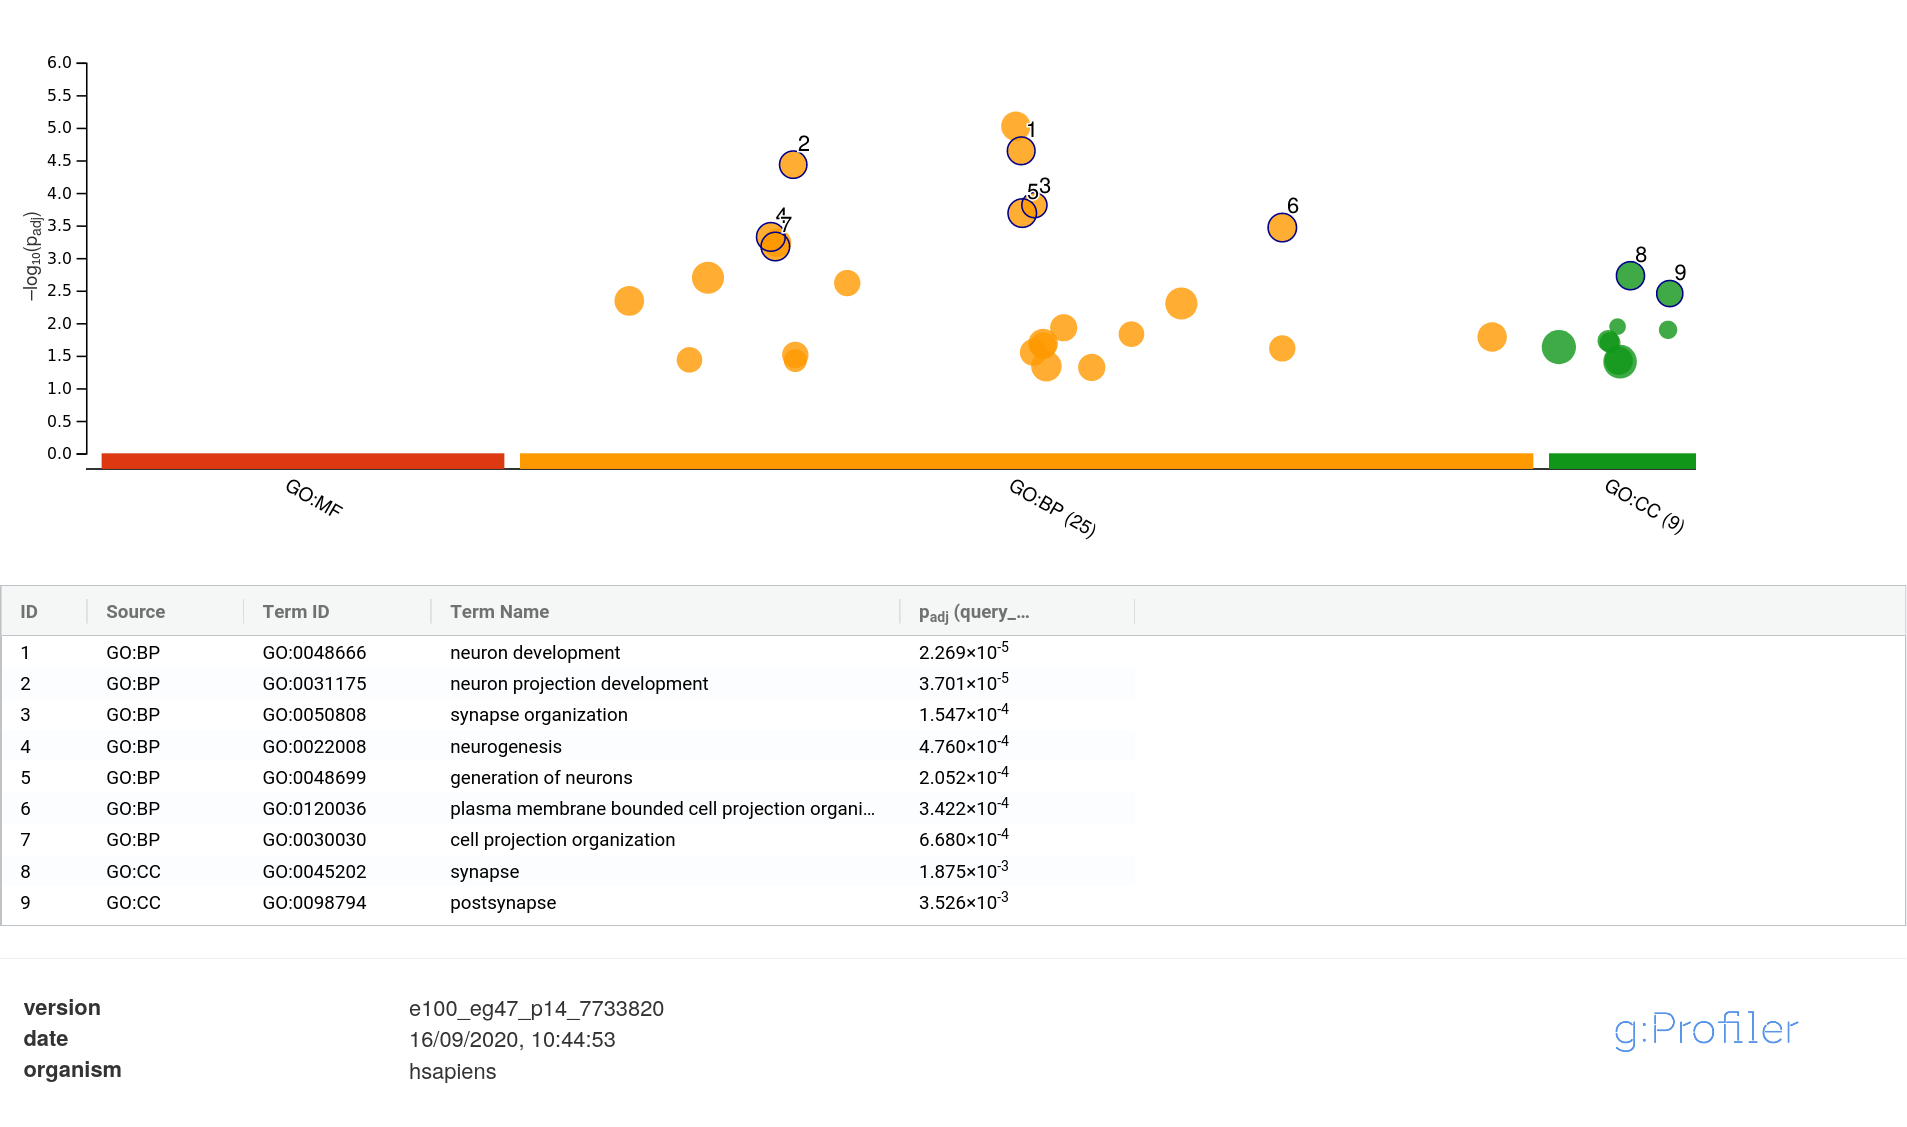
\includegraphics[width=\textwidth]{images/gprofiler/gProfiler_hsapiens_2020-09-16_09-45-55_ukbbed.png}
            %     \caption{Gene ontology enrichment Education\textsubscript{Discovery g profiler} Selected genes}
            %     \label{fig:gprofiler education discovery}
            % \end{figure}
        
            \begin{figure}
                \centering
                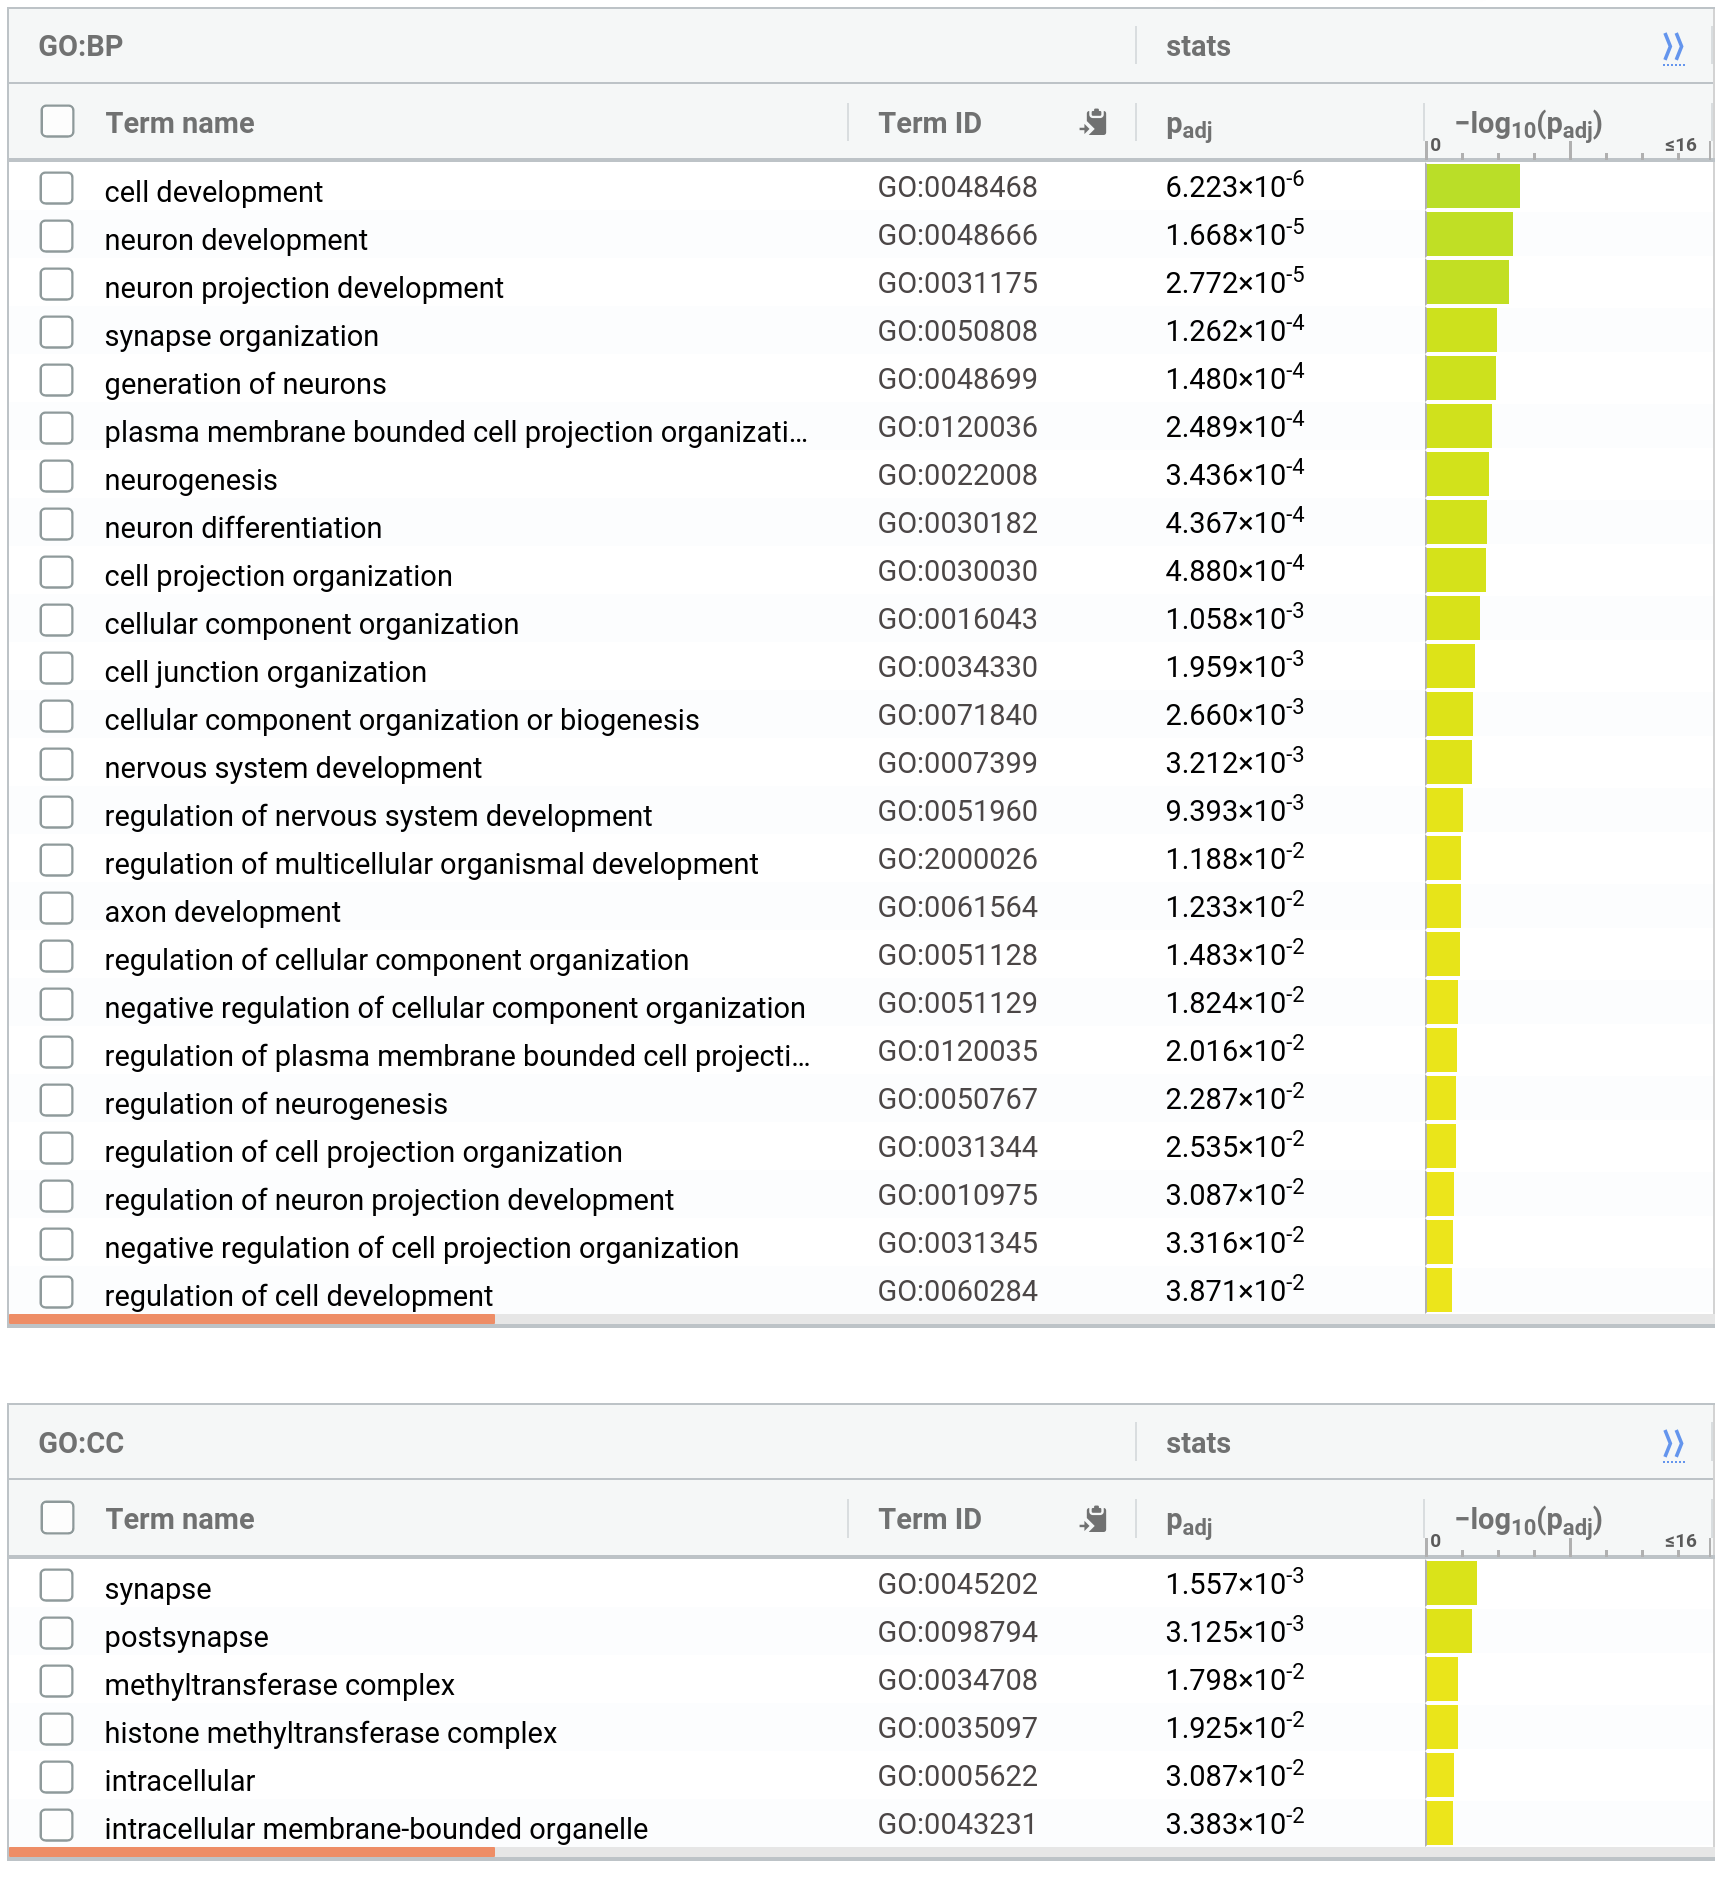
\includegraphics[width=\textwidth]{images/gprofiler/all_terms/ukbbed_allterms.png}
                \caption{Table of all terms Education Discovery gProfiler}
                \label{fig:table all terms Education Discovery gProfiler}
            \end{figure}

  \subsubsection{SynGO}
  \begin{table}[]
    \centering
    \begin{tabular}{llll}
    \toprule
    Cellular component & n & p & FDRq\\
    \midrule
    synapse organization&	15&	$7.44\times10^{-6}$&	$6.69\times10^{-5}$\\

process in the synapse&	20	&$4.06\times10^{-3}$	&0.0183\\
trans-synaptic signaling&	6&	0.0234&	0.0428\\
synapse adhesion between pre- and post-synapse&	3	&0.0146&	0.0428\\
regulation of synapse assembly&	3&	0.0238&	0.0428\\

synapse assembly&	4&	0.0289	&0.0433\\
      \bottomrule  
    \end{tabular}
    \caption{SynGO Biological Process Education\textsubscript{Discovery}}
    \label{tab:syngo biological process education discovery}
\end{table}
  
  \begin{table}[]
    \centering
    \begin{tabular}{llll}
    \toprule
    Cellular component & n & p & FDRq\\
    \midrule
 synapse&	23&	0.00451&	0.0316\\
postsynapse	&14	&0.0245&	0.0858\\
\bottomrule
\end{tabular}
\caption{syngo CC Education Discovery}
\label{tab:syngo CC Education discovery}
\end{table}
            % \paragraph{BP Education Discovery} One term synapse	 n= 23	p=2.64e-3	q=0.0185
            
            % \paragraph{CC Education Discovery}
            % 6 significant terms. See table~\ref{tab:syngo cc ukbb ed}
            
            
 
 
 
 Synapse, GO:0045202, was the only enriched cellular component term using SynGO (table~\ref{tab:syngo CC Education discovery}).
SynGO annotates only 23 of the significant genes to synapse, compared to 40 genes in ToppGene table~\ref{tab:Cellular component Education Discovery ToppGene top10 results Bonfe}. Six biological process terms are enriched,  including synapse organisation GO:0050807( table~\ref{tab:syngo biological process education discovery}). Fifteen terms are annotated synapse organisation by SynGO compared with 19 in toppgene (table~\ref{tab:Biological Process Education Discovery ToppGene top10 results BY} but the limited ontology results in a more significant FDR ($6.69\times10^{-5}$ compared to 0.018). These results show both the benefits and limitations of specialised ontologies.      \footnote{      NOte synapse organisation GO:0050807) has 15 annotated terms with FDR q $3.97\times10^{-5}$ compared to regulation of synapse organisation 11 of 229 P $0.943\times{10^-5}$ FDR 0.0483 in PANTHER GO:0050807
 See table~\ref{tab:syngo biological process education discovery}}

 
 Using FUMA to analyse gene expression the GWGAS significant Education\textsubscript{Replication} genes are over-represented amongst  differentially expressed genes up-regulated in the brain using GTEx (figure~\ref{fig:ukbbed gtex}). This is the only sample in which this is the case (see figure~\ref{fig:FUMA gtex deg samples multiple} and figure~\ref{fig:deg_upref_sample_gtex_gener} which shows only over-representation. 

% \subsubsection{Summary of Education Discovery}
% ToppGene and gprofiler No Molecular function

% Genes association with ID

% MF nil in PANTHER
% BP neurogenesis and synapse organisation and neuron projection

% CC MHC (which is assoc type II dm) ER PSD and post synapse, neuron projection
%         \subsubsection{Summary of above findings}

 \begin{figure}
  \begin{subfigure}{12cm}
    \centering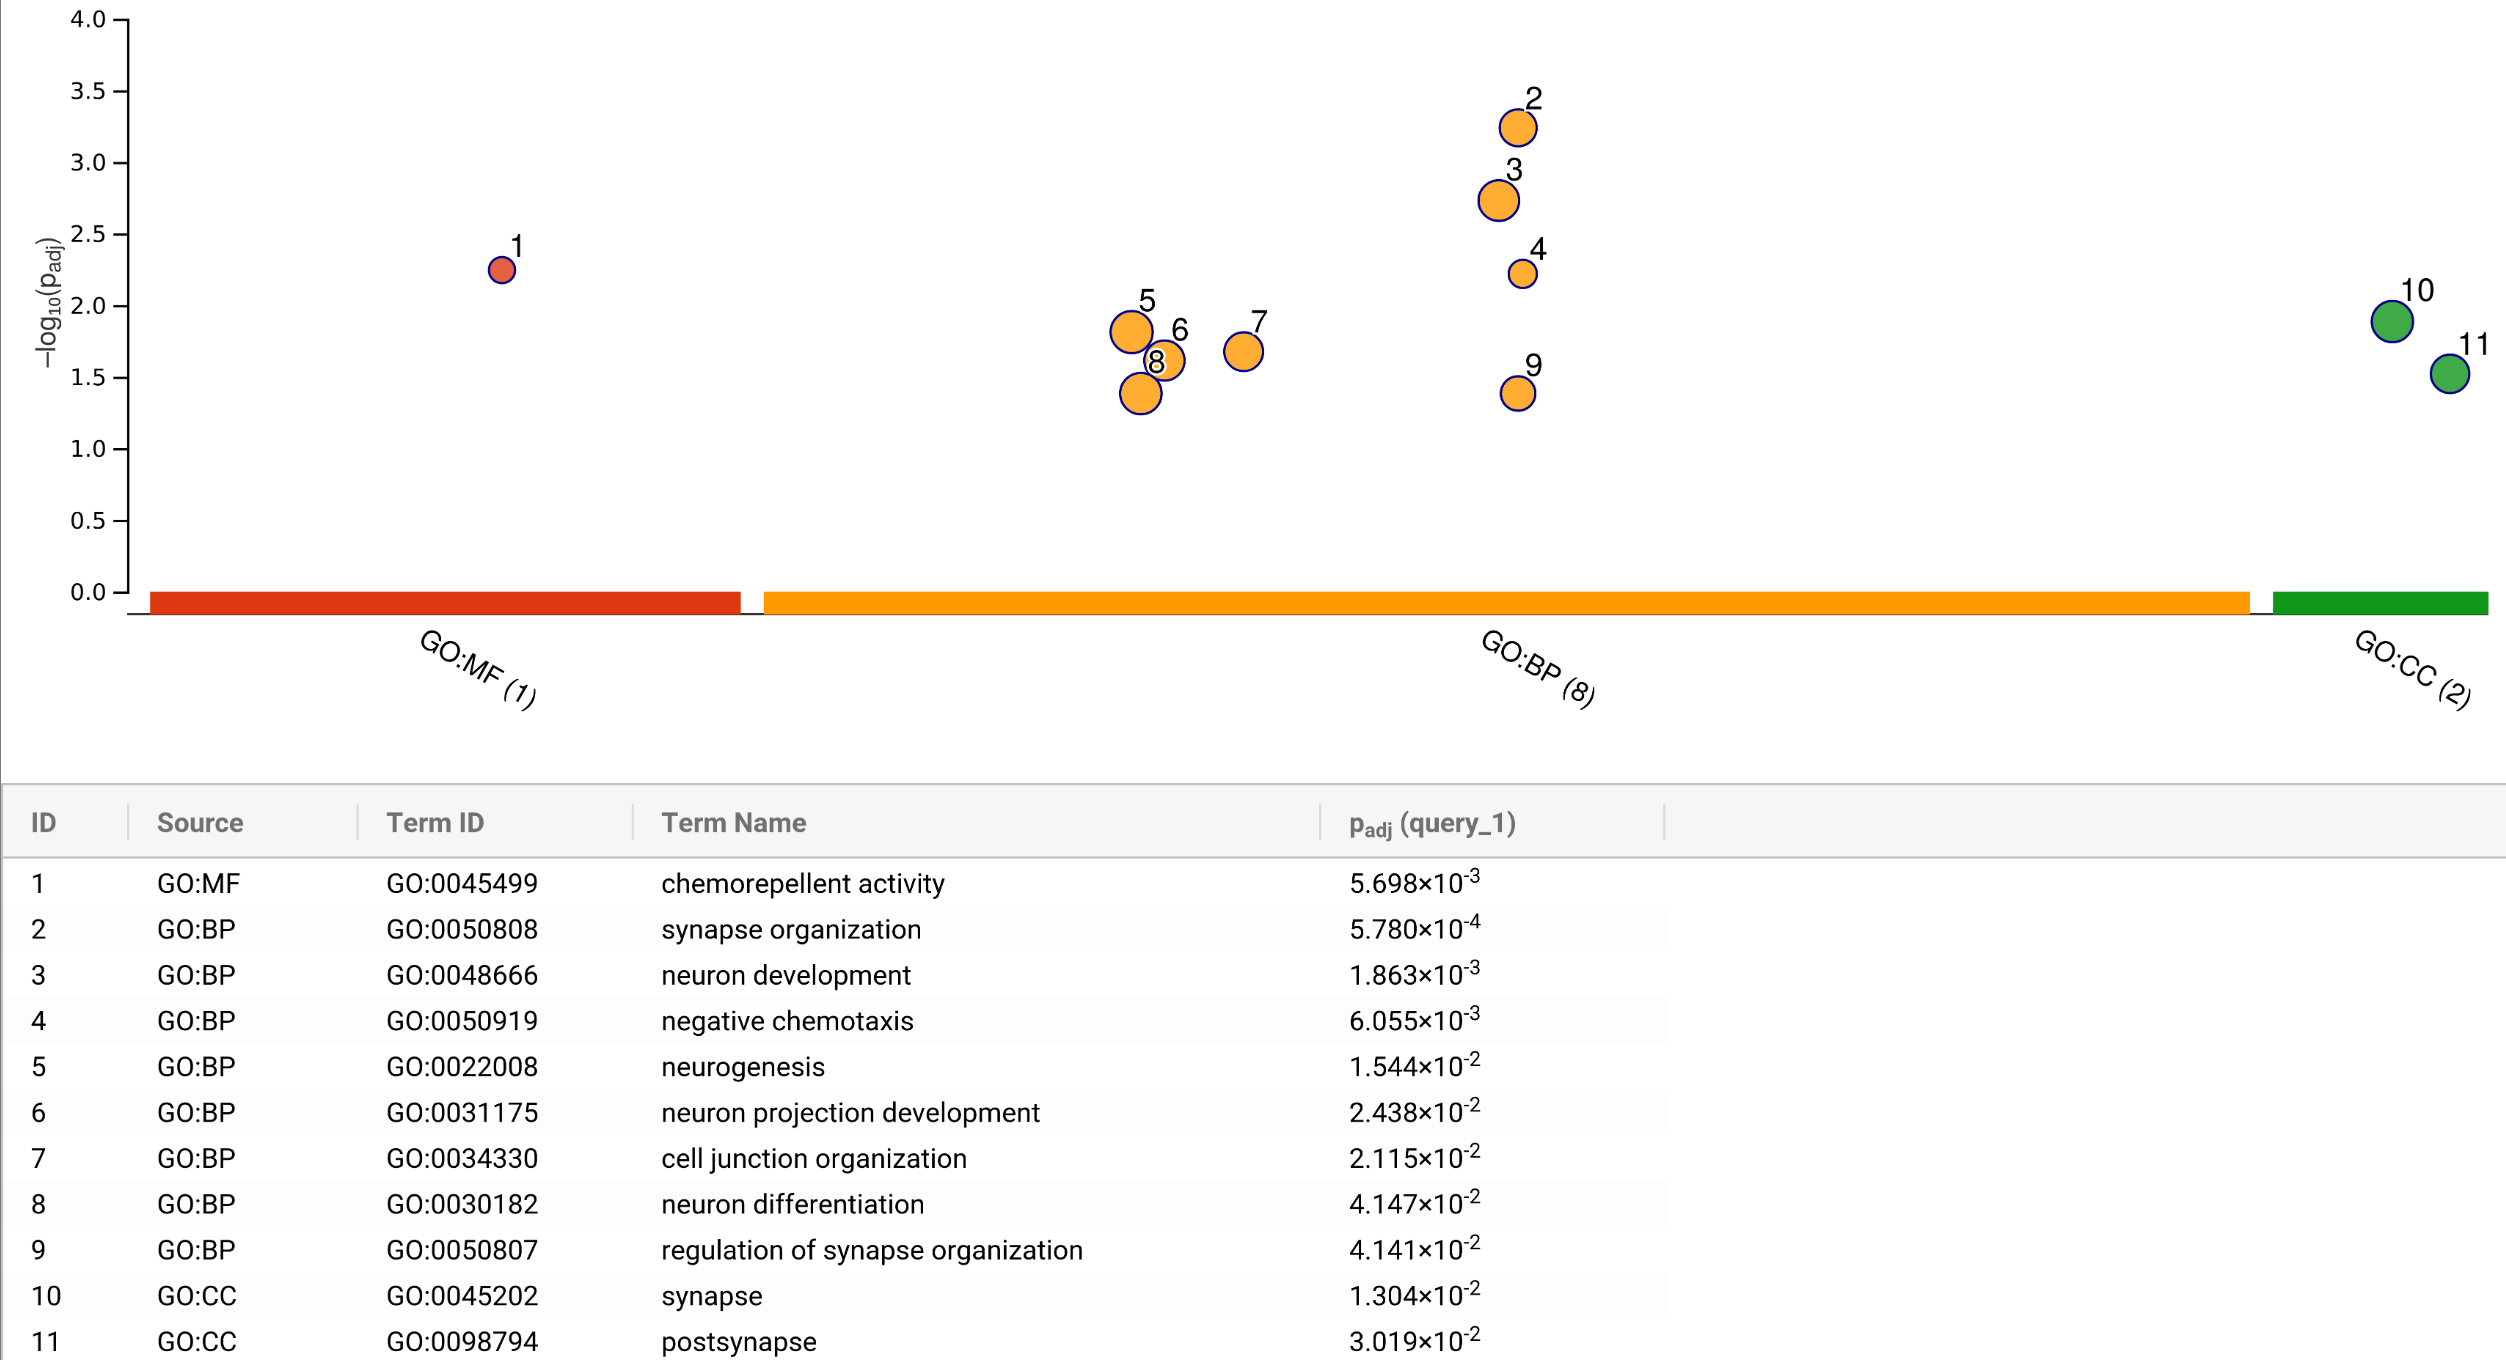
\includegraphics[width=11cm]{images/gprofiler/gprofiler_ea2_clip.png}
    \caption{gProfiler. Education Replication}
    \end{subfigure}
    
  \begin{subfigure}{12cm}
    \centering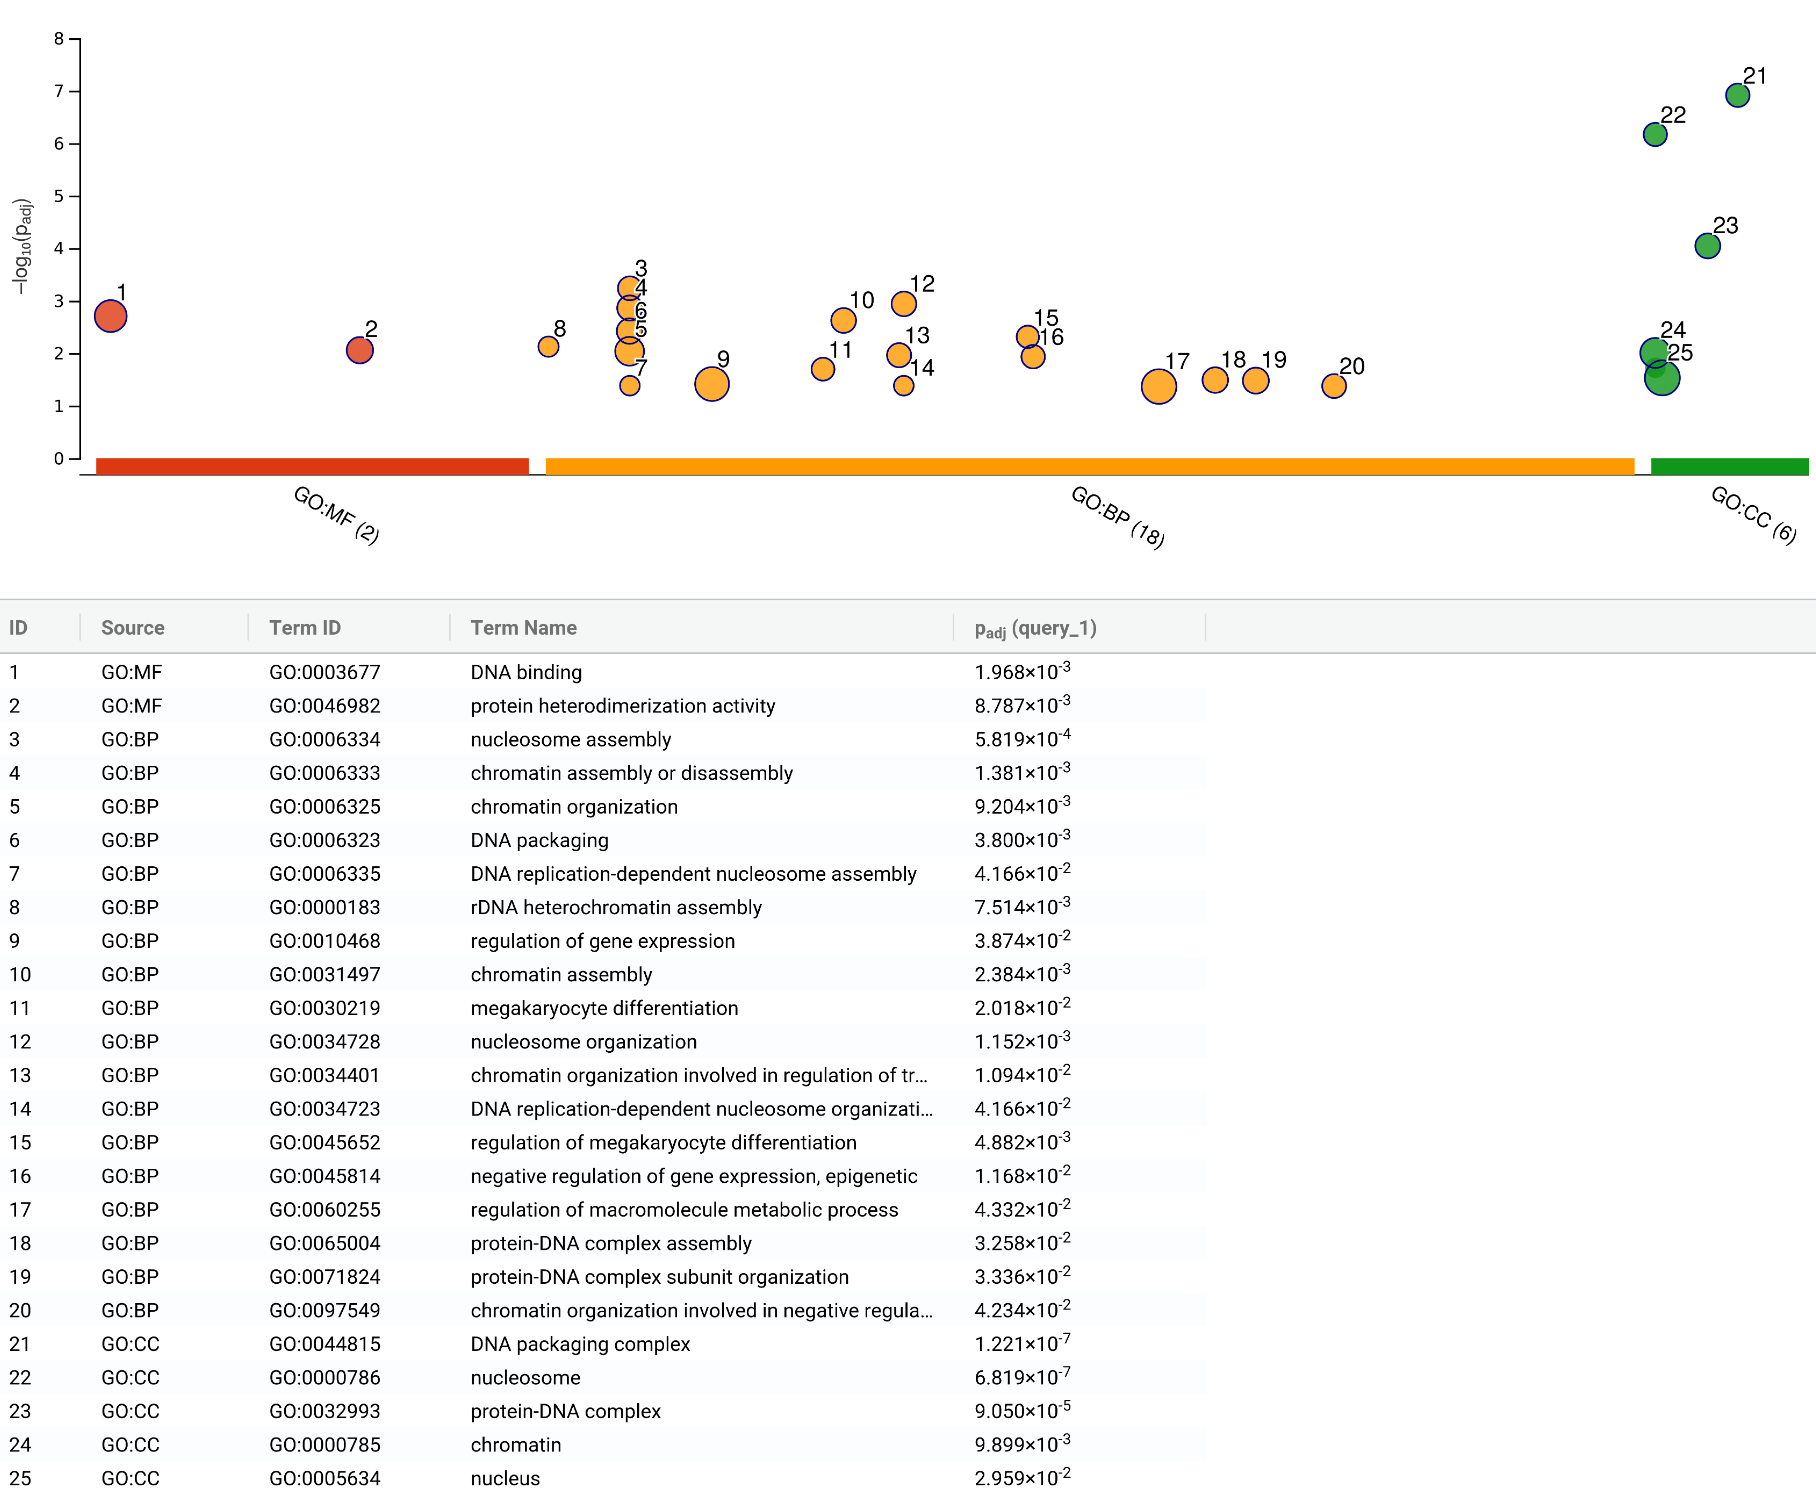
\includegraphics[width=11cm]{images/gprofiler/gprofiler_ukbbint_clip.png}
    \caption{gProfiler Intelligence Discovery}
  \end{subfigure}
 
  \begin{subfigure}{12cm}
    \centering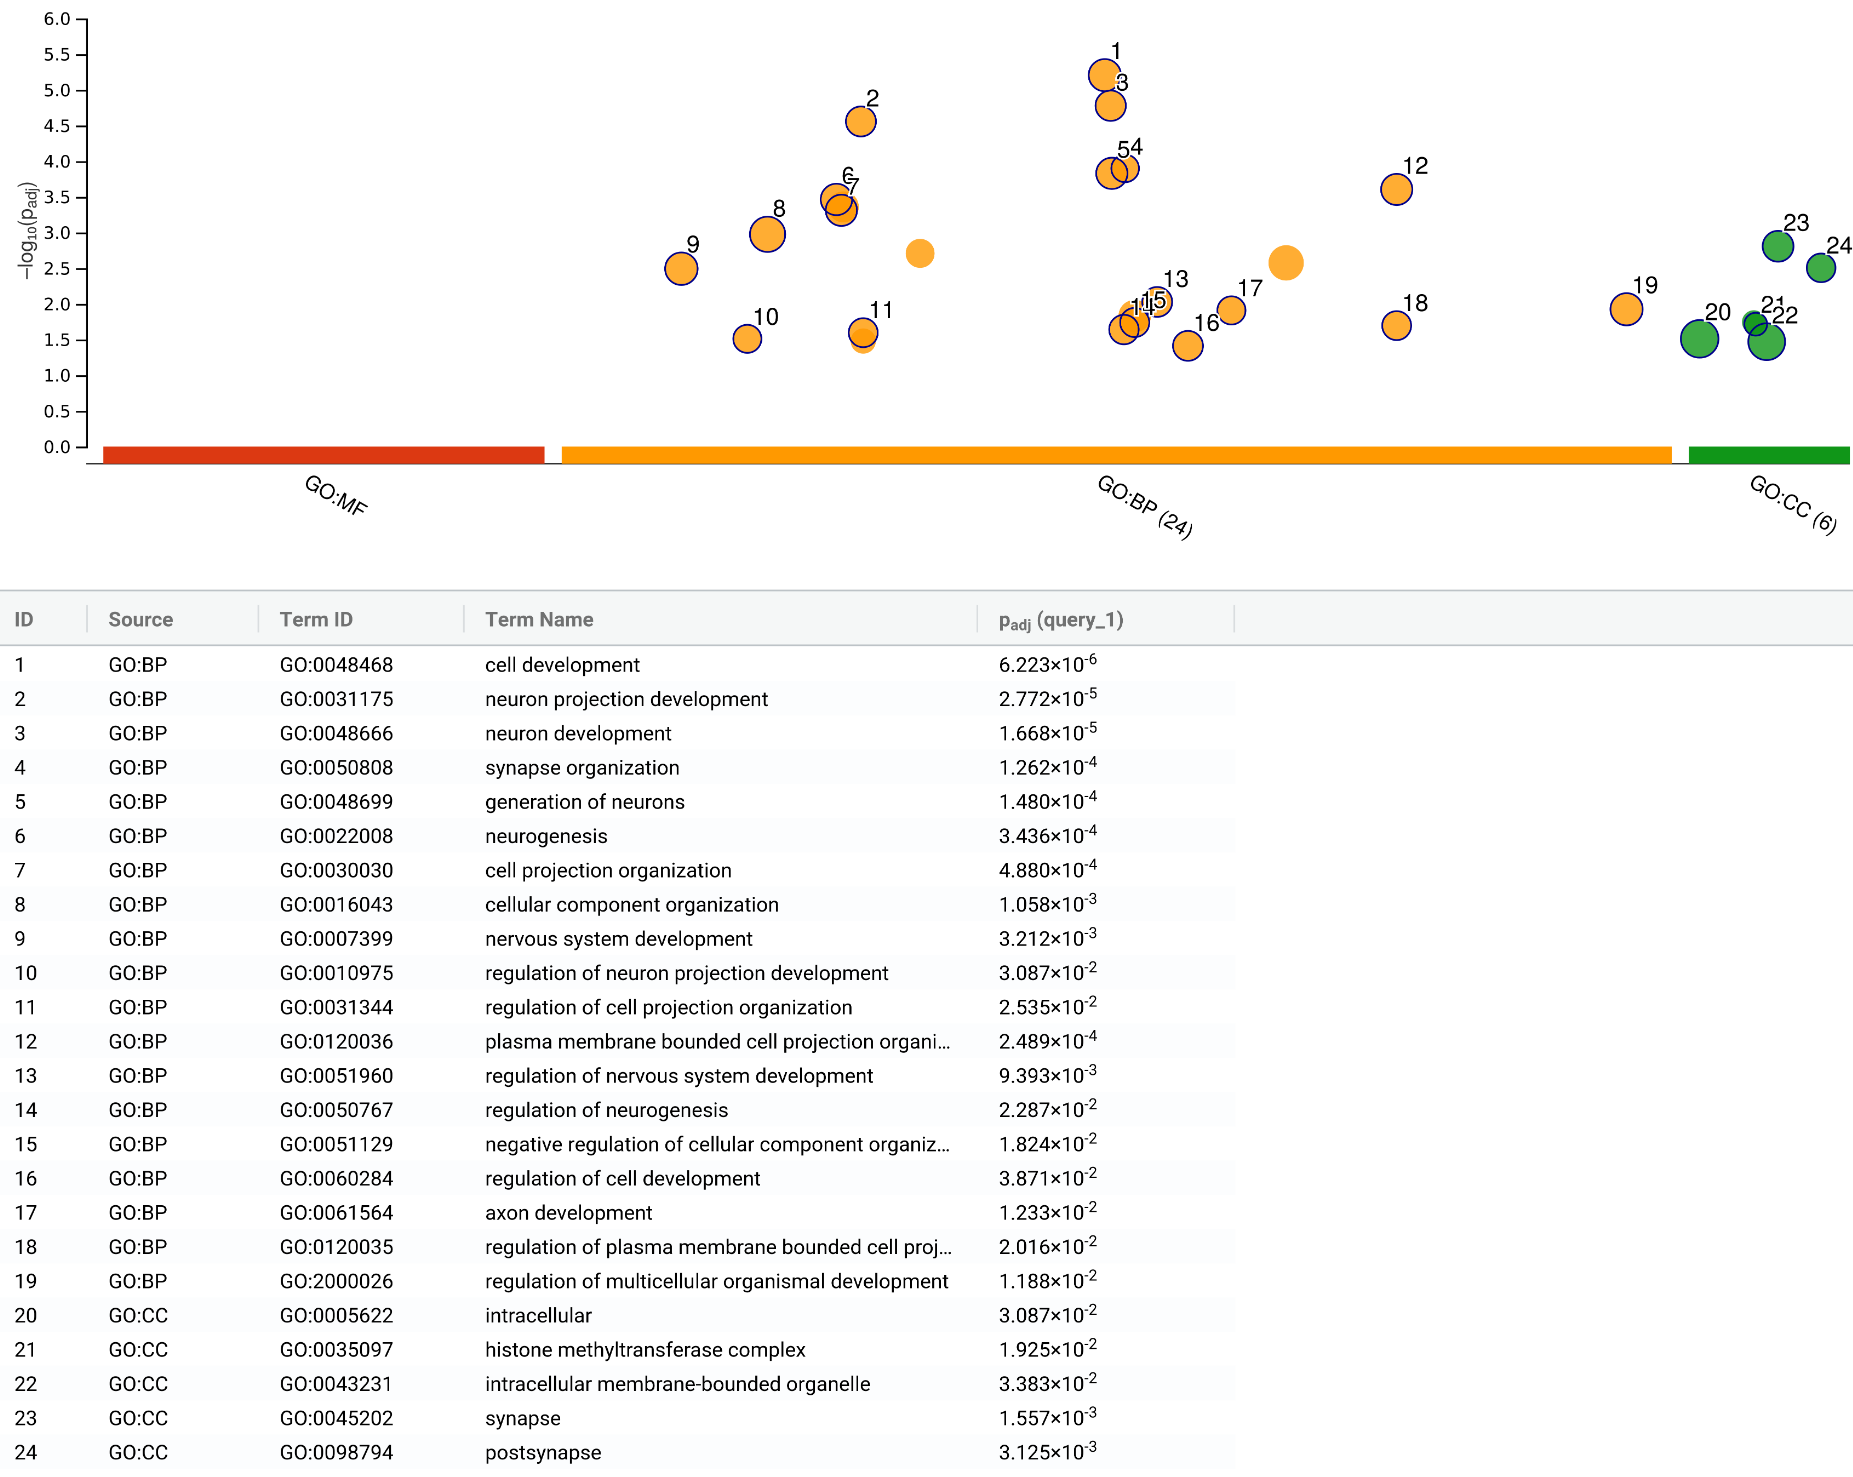
\includegraphics[width=11cm]{images/gprofiler/gprofiler_eukbbed_clip.png}
    \caption{gProfiler Education Discovery}
  \end{subfigure}
  \caption{Gene Ontology enrichment of significant genes using gProfilers}
  \label{fig:gProfiler 3 samples}
  
\end{figure}

\begin{figure}
    \centering
    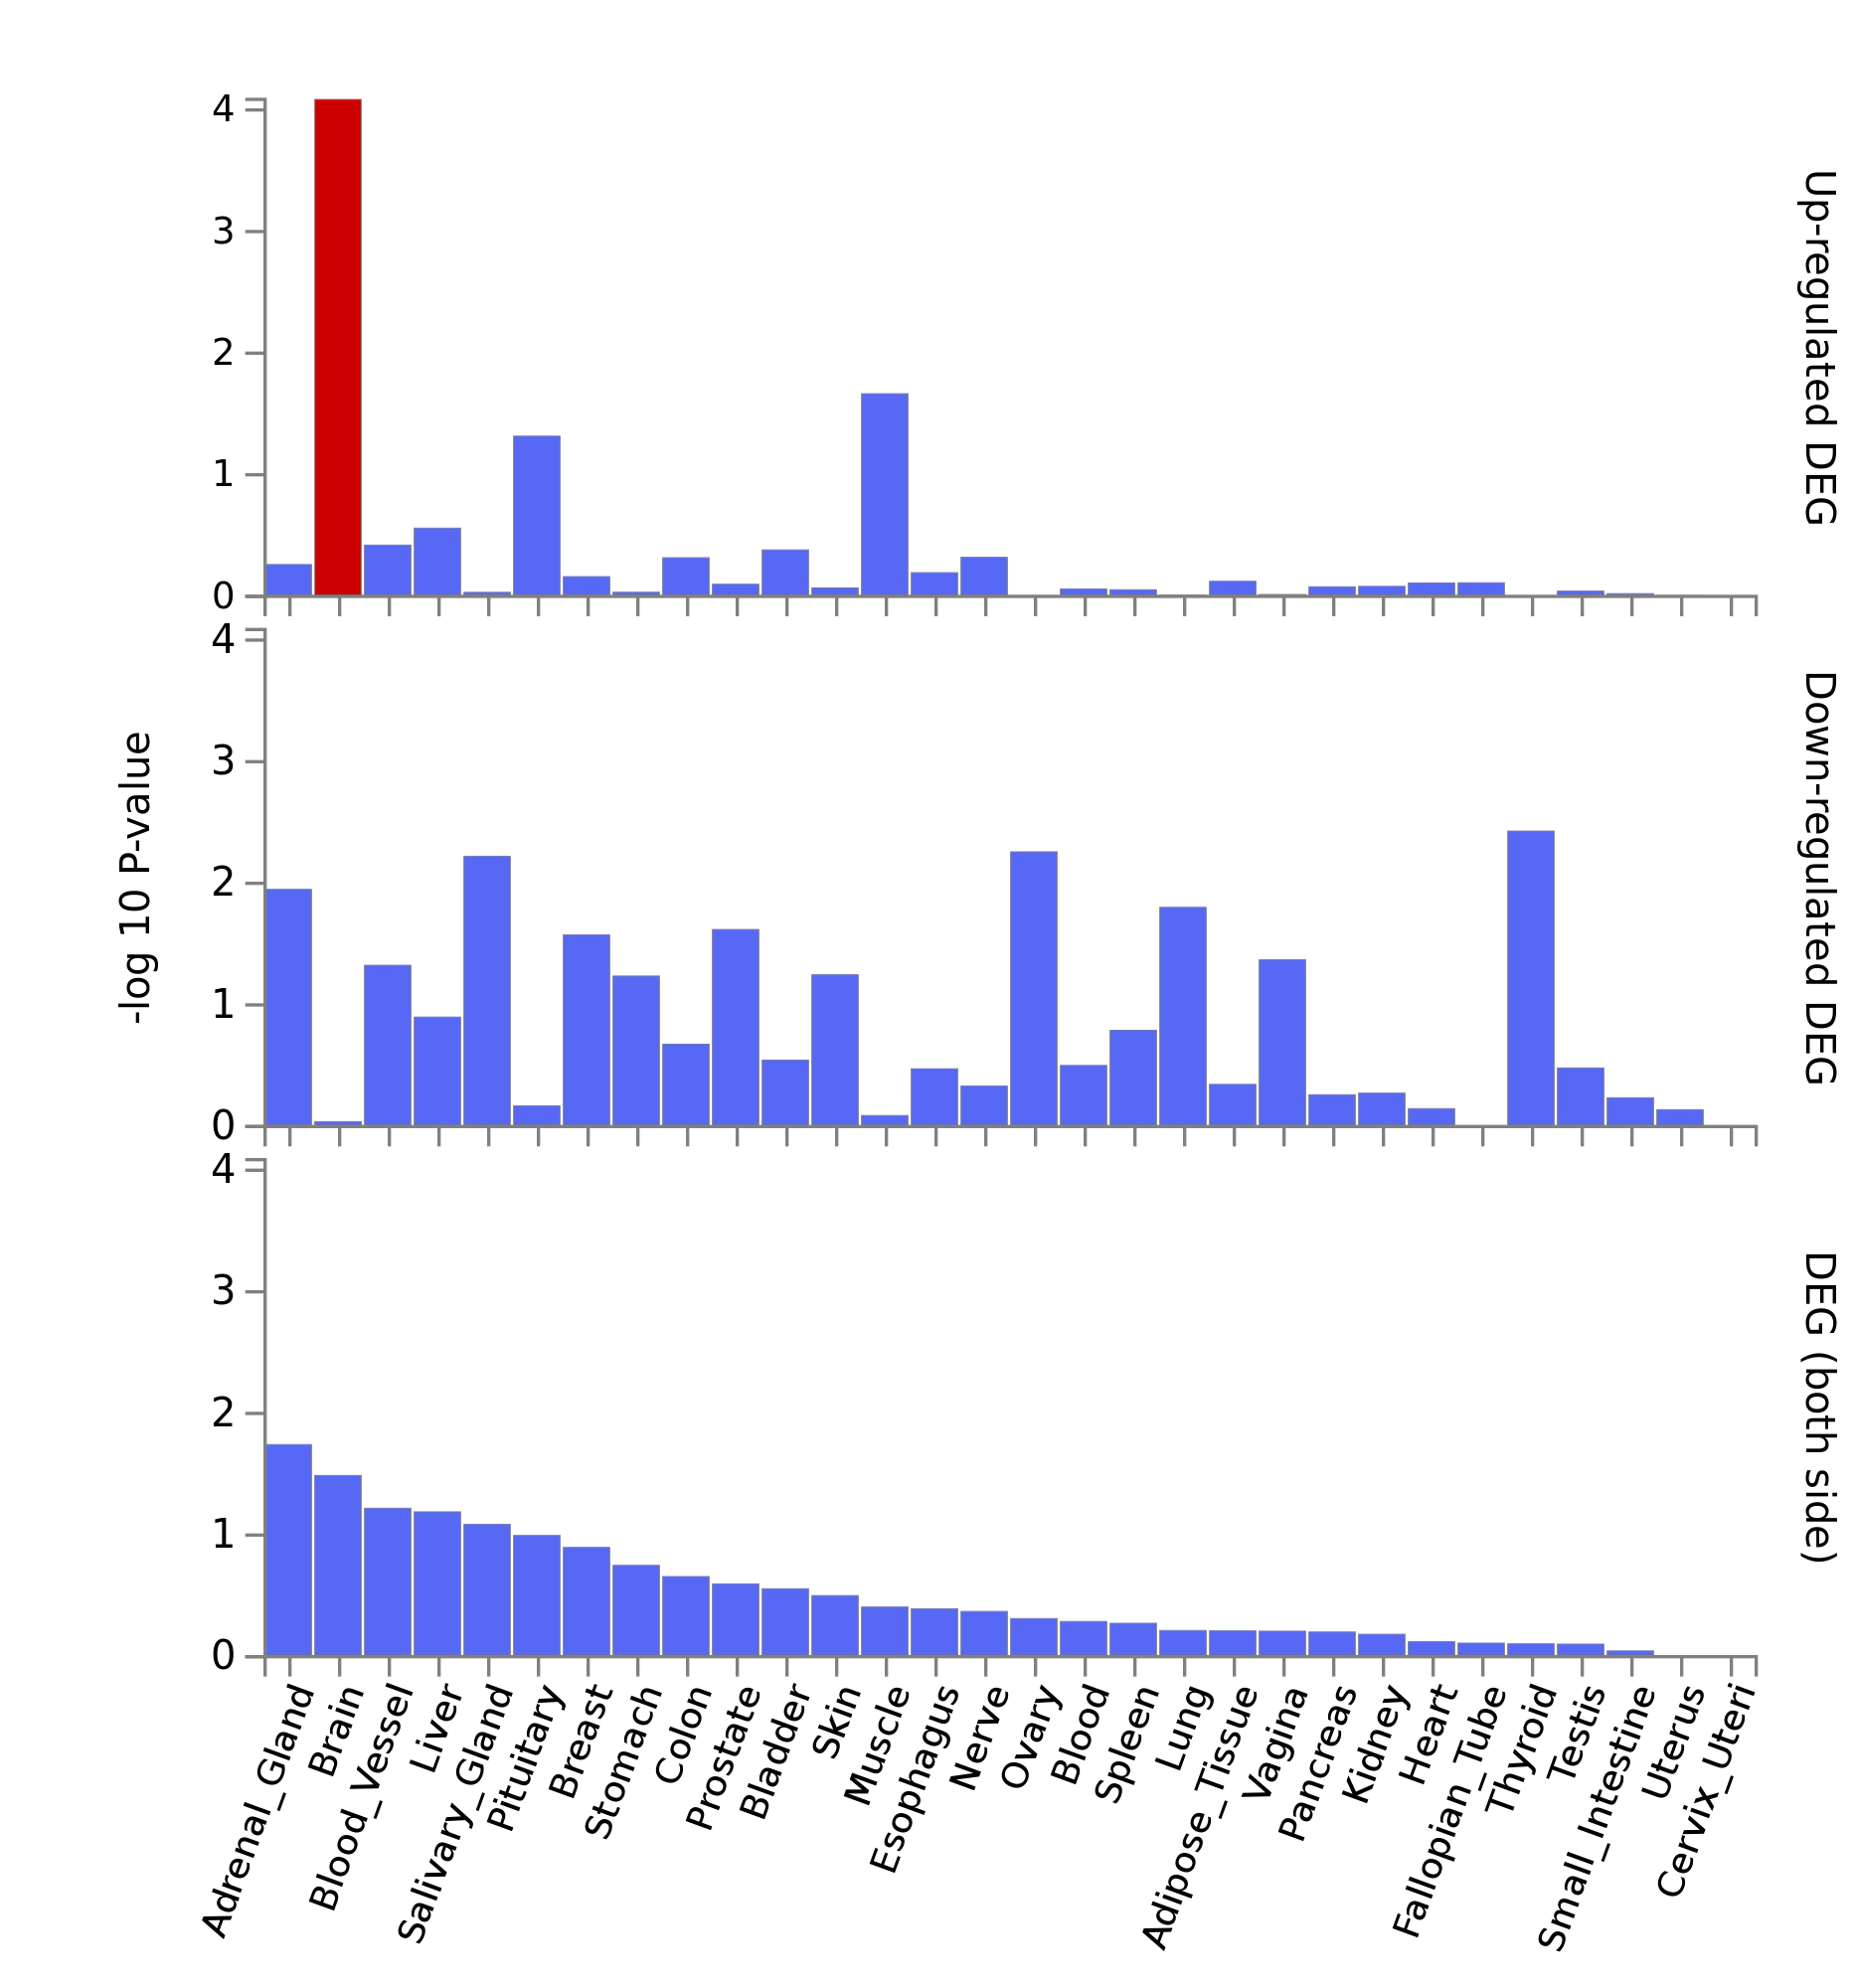
\includegraphics[width=\textwidth]{images/FUMA_plots/gtex_v8_ts_general_FUMA_gene2func_UKBBEd_syn_protein_bp_sig.png}
    \caption{Gtex General UKBBEd Synaptic significant.png}
    \label{fig:ukbbed gtex}
\end{figure}


\begin{figure}
    \centering
    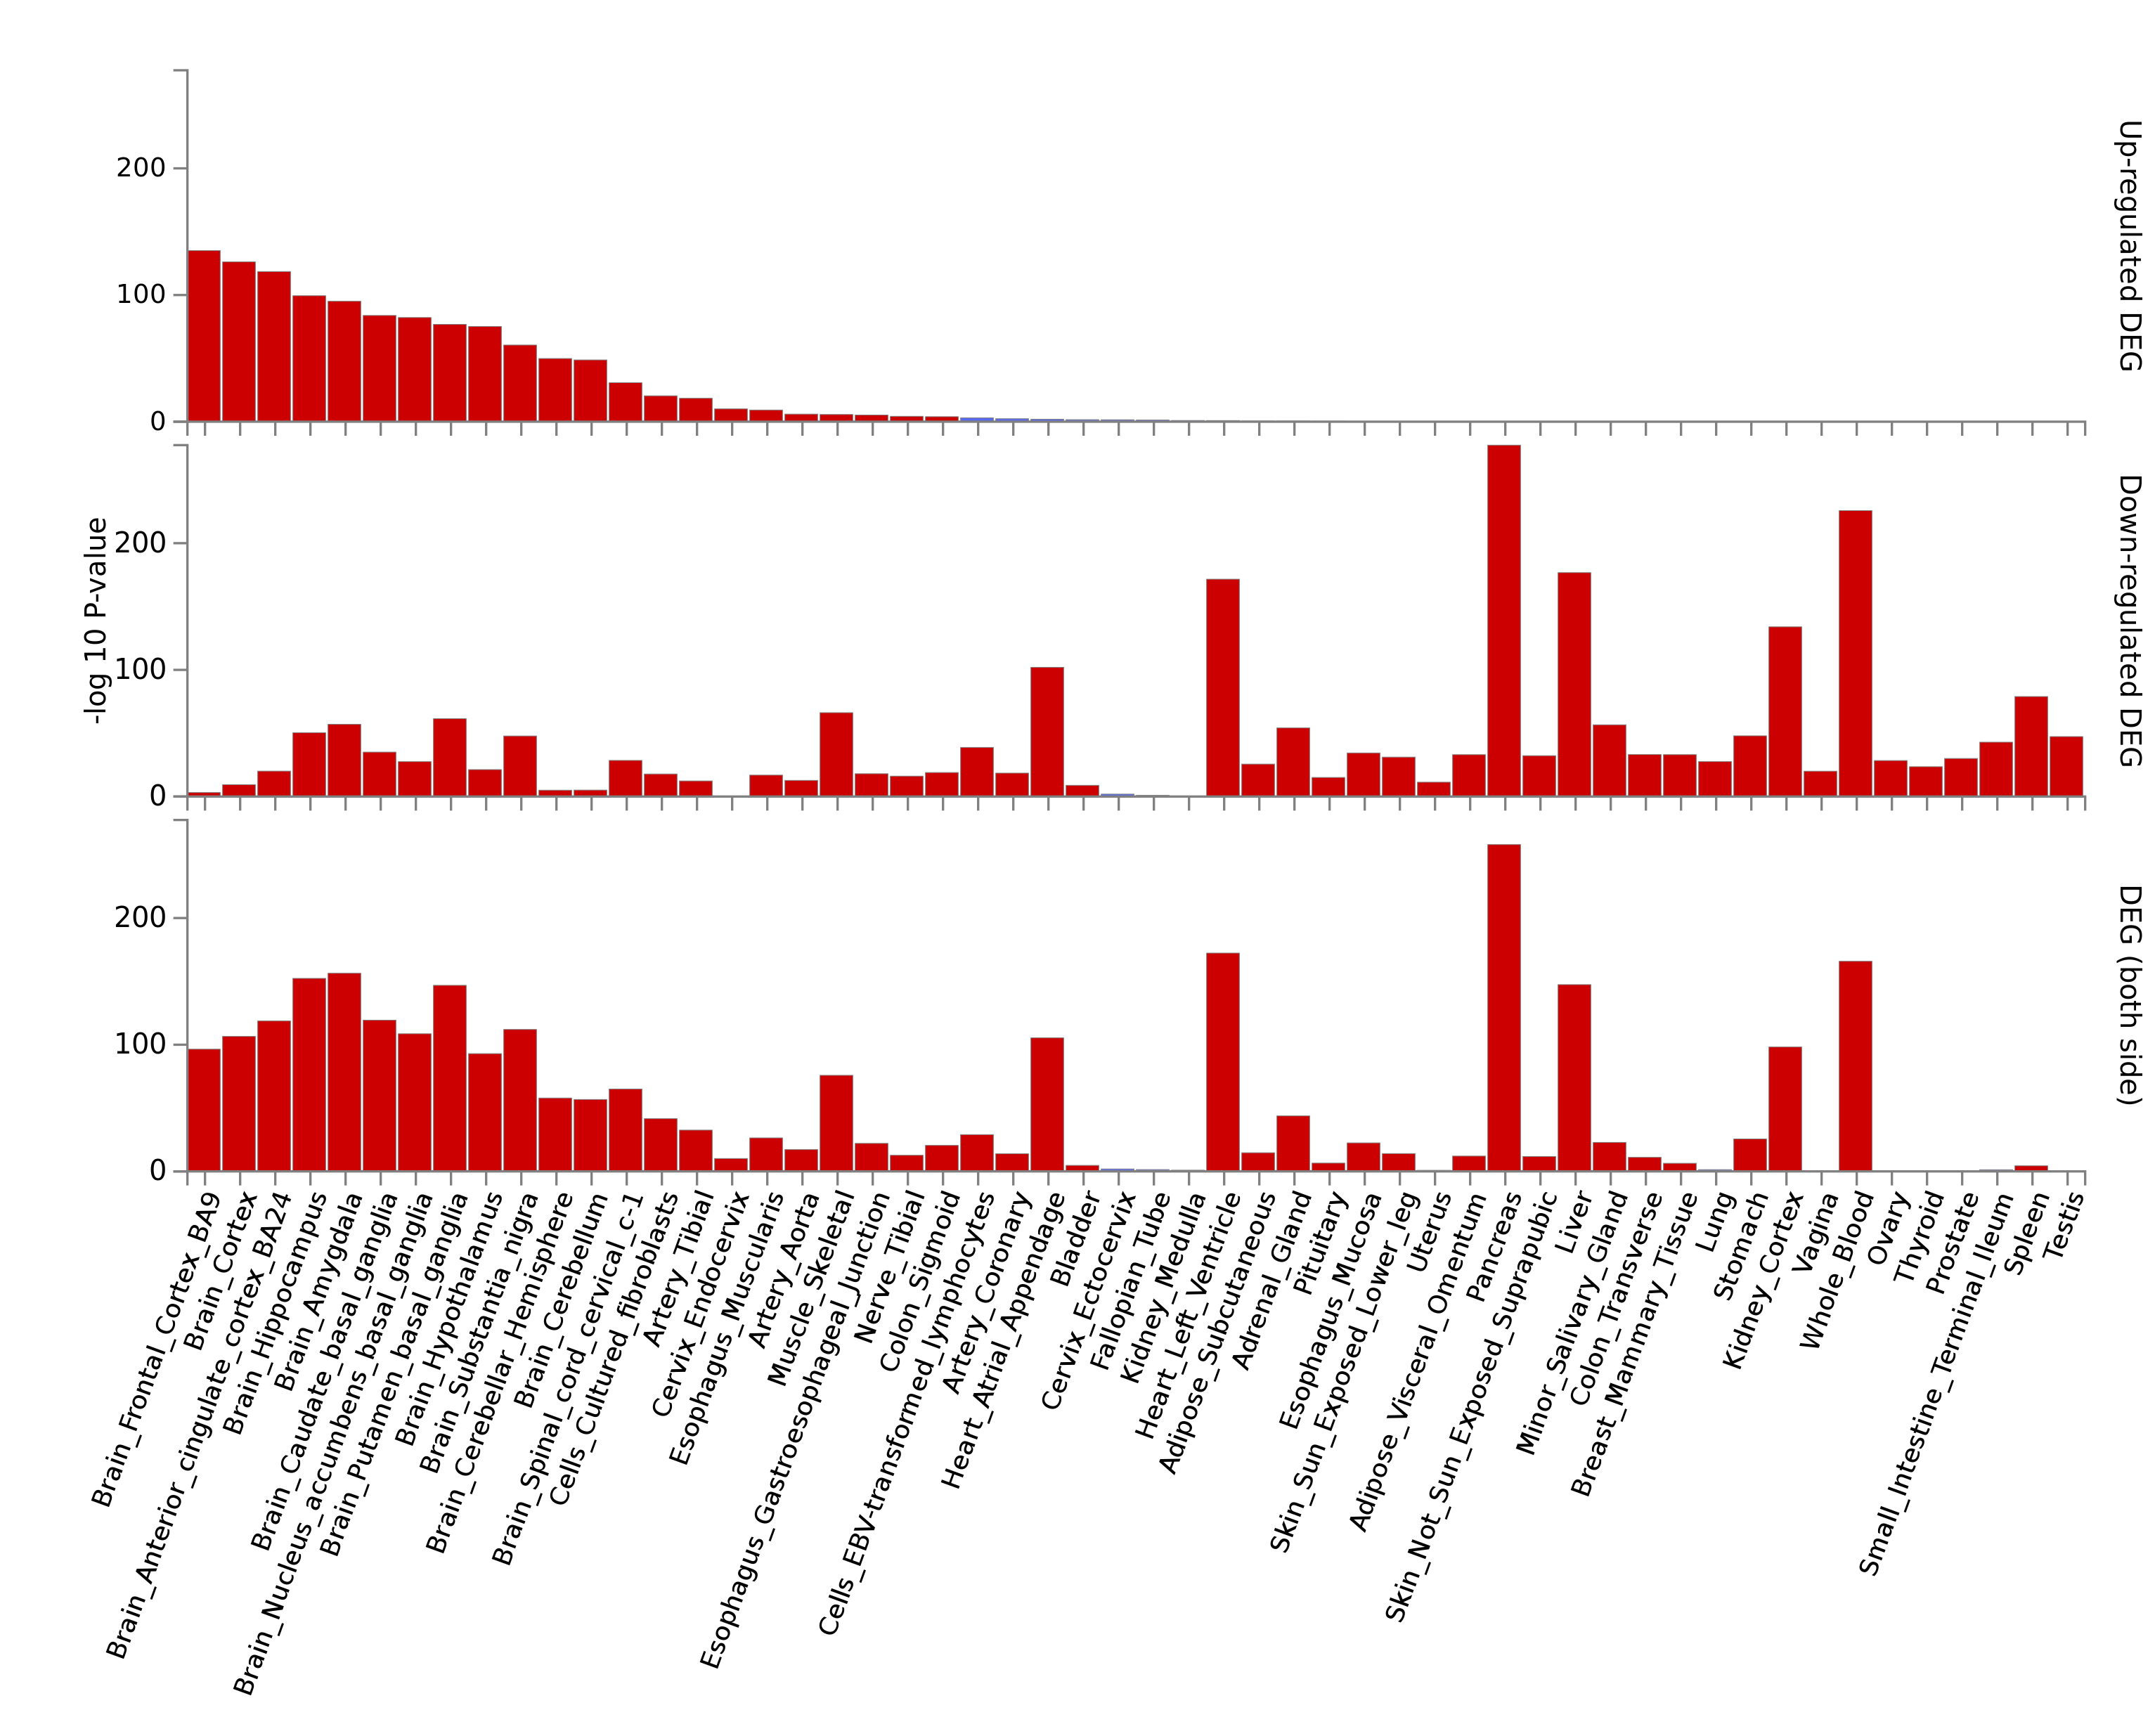
\includegraphics[width=\textwidth]{images/FUMA_plots/gtex_v8_ts_FUMA_PSP_gtex.png}
    \caption[GTEx All PSP]{GTex all PSP. Note top row of upregulated genes. Shows that signal from expanded PSP is very specific to CNS expression. Red significant. Y axis -log10 of p value. Hypergeometric test of genes differentially expressed from pre-created list see FUMA \cite{watanabe2017functional} for details (two sided Bonferroni corrected p versus all labels with cut off fold change) }
    \label{fig:gtex all PSP}
\end{figure}
\clearpage


\begin{figure}
    \centering
    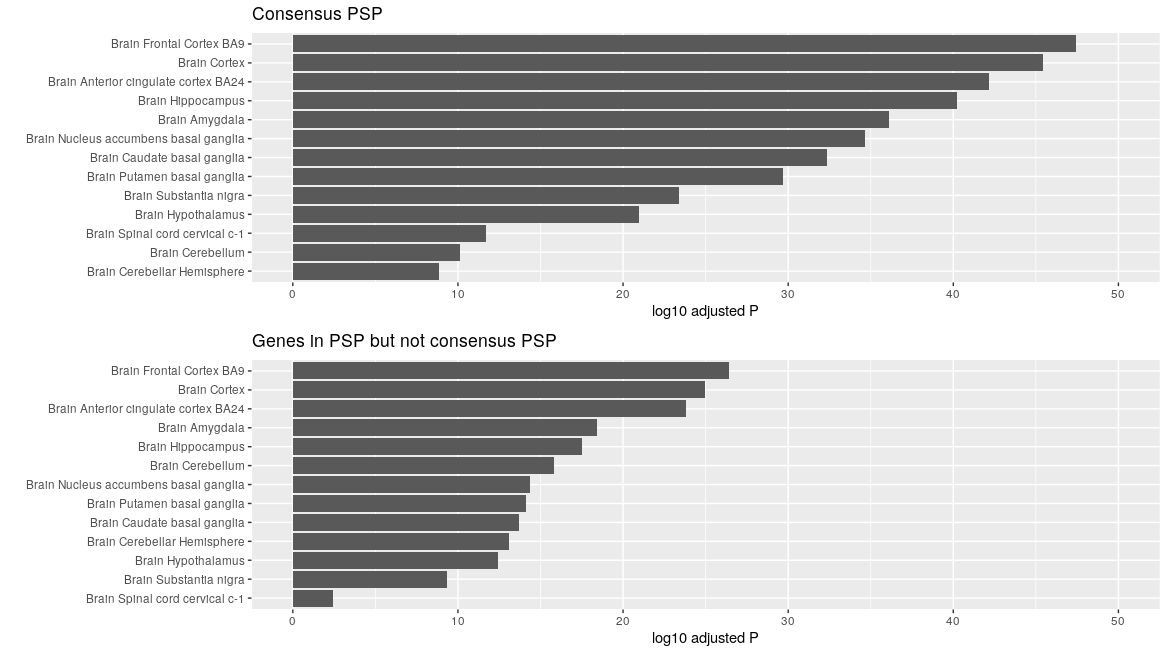
\includegraphics[width=\textwidth]{images/chapter2/ggplot/Rplot_consensusgtex.png}
    \caption{Differentially expressed genes over representation analysis in Gtex. Top panel genes in consensus PSD $n=1312$. Lower panel genes not in consensus PSD but in PSP.\url{source('~/RProjects/paper_xls_output/R/chapter_2/FUMA/plot_gtex/plot_consensus_multiplot.R')}}
    \label{fig:deg_gtex_psp}
\end{figure}



\begin{figure}
    \centering
    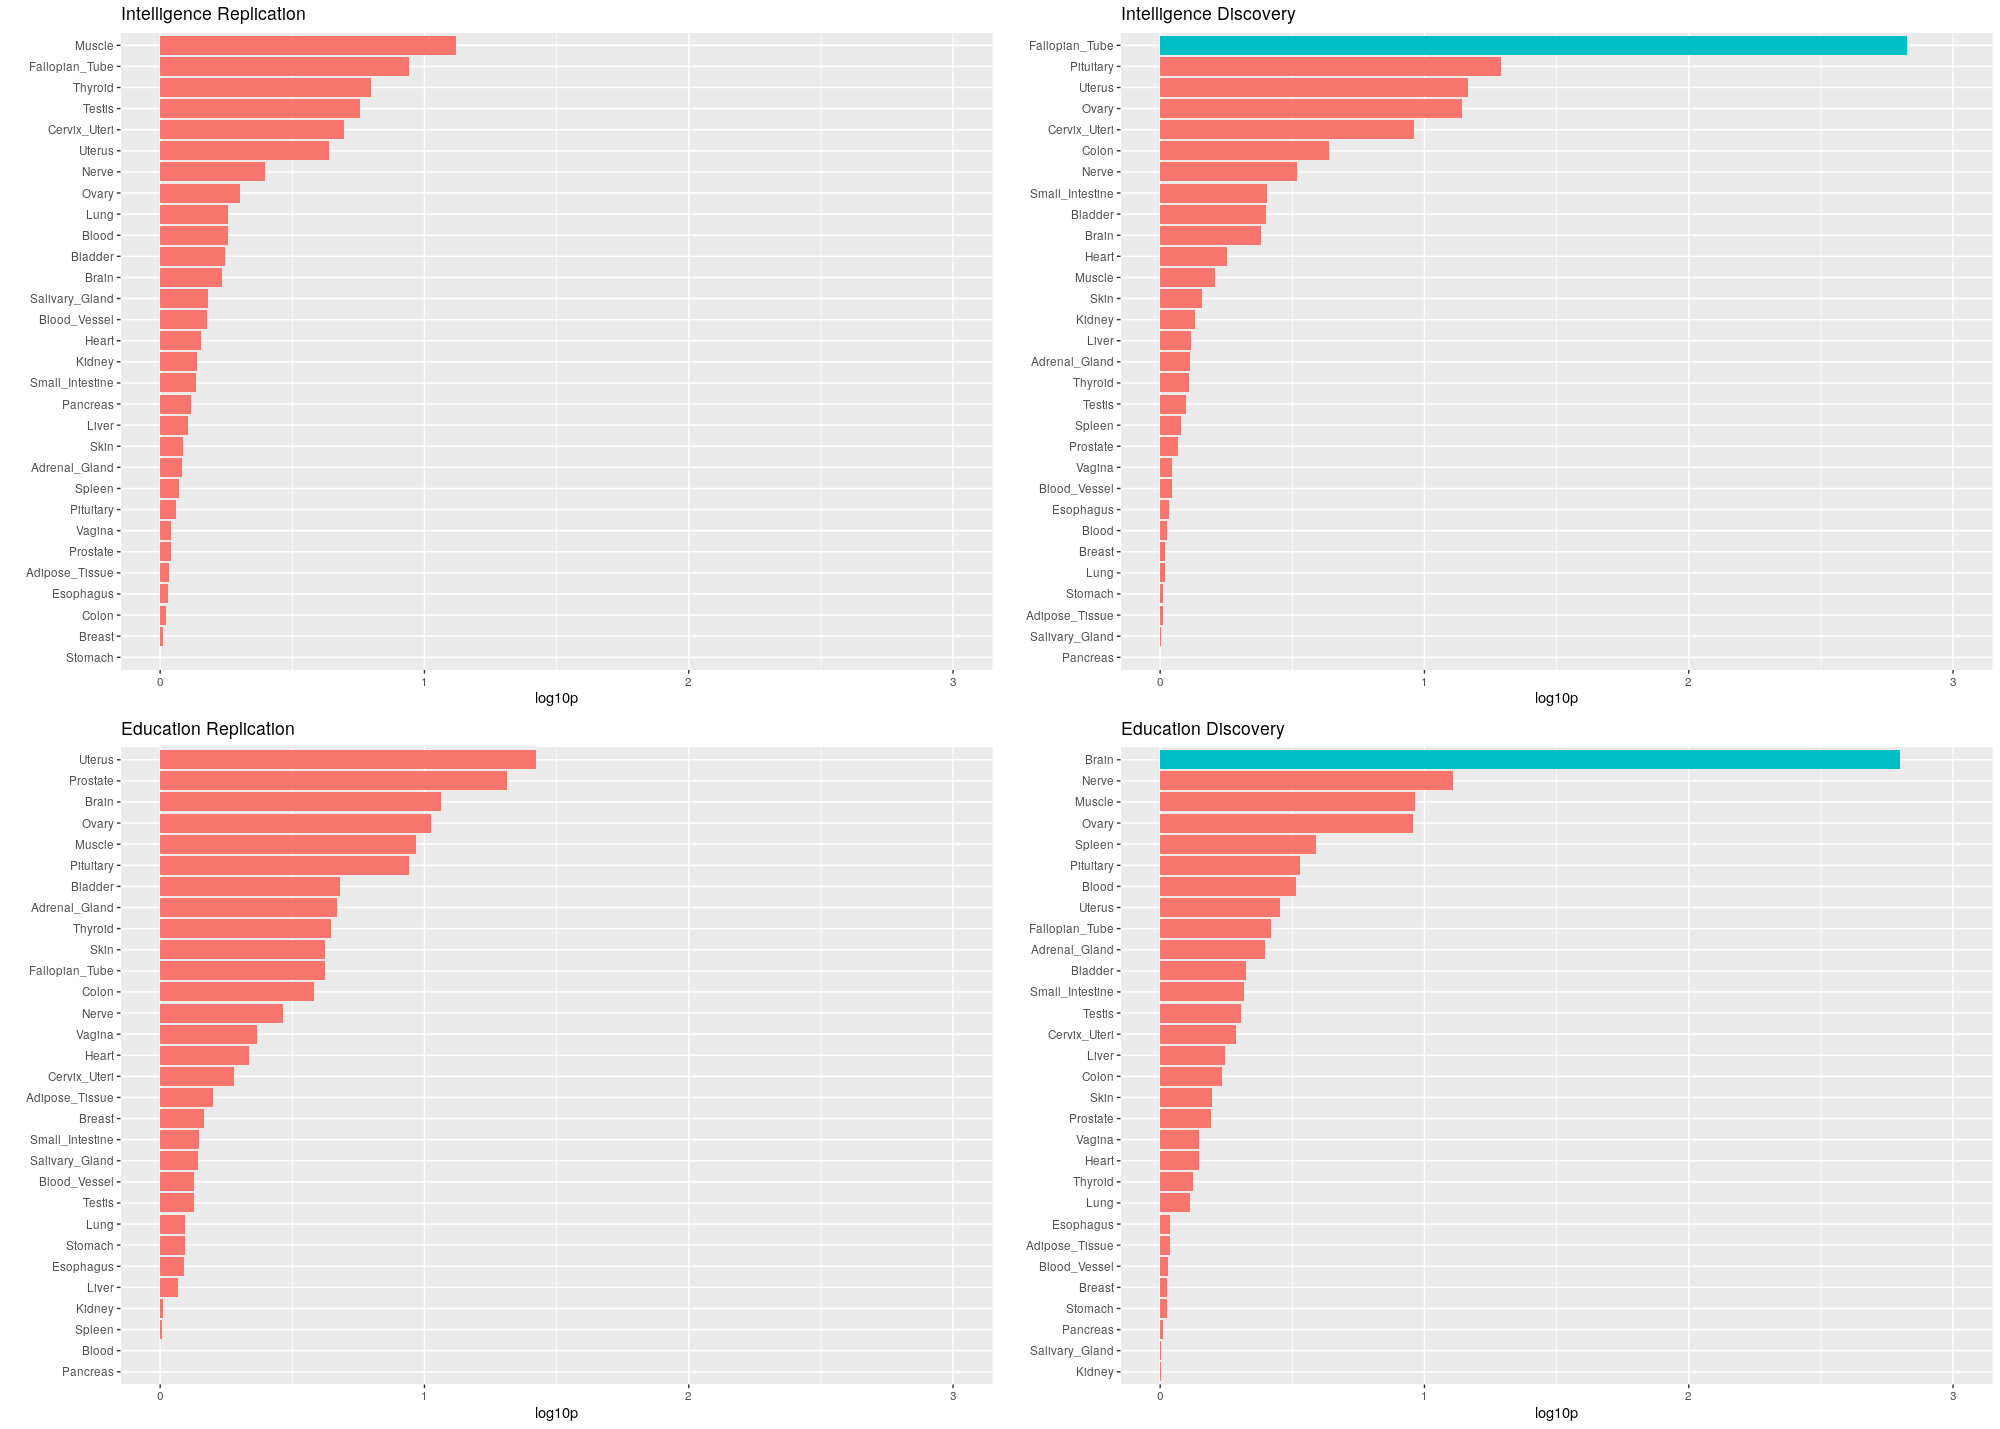
\includegraphics[width=\textwidth]{images/chapter2/ggplot/ggplot_FUMA/Rplot_upregulated_general.png}
    \caption{Over representation of differentially expressed genes (up regulated) amongst significant genes at GWGAS for each of the samples clockwise from top left Intelligence Replication, Intelligence Discovery, Education Discovery and Education replication using FUMA to perform over representation. Gene expression data GTEx v8. x axis is -log10 transform of p value for cumulative hypergeometric test. Significant tissues are shown in cyan. The only sample with over representation of genes with up-regulated differential expression in the brain is Education\textsubscript{Replication} \url{source('~/RProjects/paper_xls_output/R/chapter_2/FUMA/plot_gtex/plot_study/multiplot_samples.R')}}
    \label{fig:deg_upref_sample_gtex_gener}
\end{figure}

%%%
% \subsection{Statistical analysis}\todo{move}

% Correction for multiple testing - by package or using adjust\_p in R. Statistical tests in R version . 

 \begin{figure}
  \begin{subfigure}{8cm}
    \centering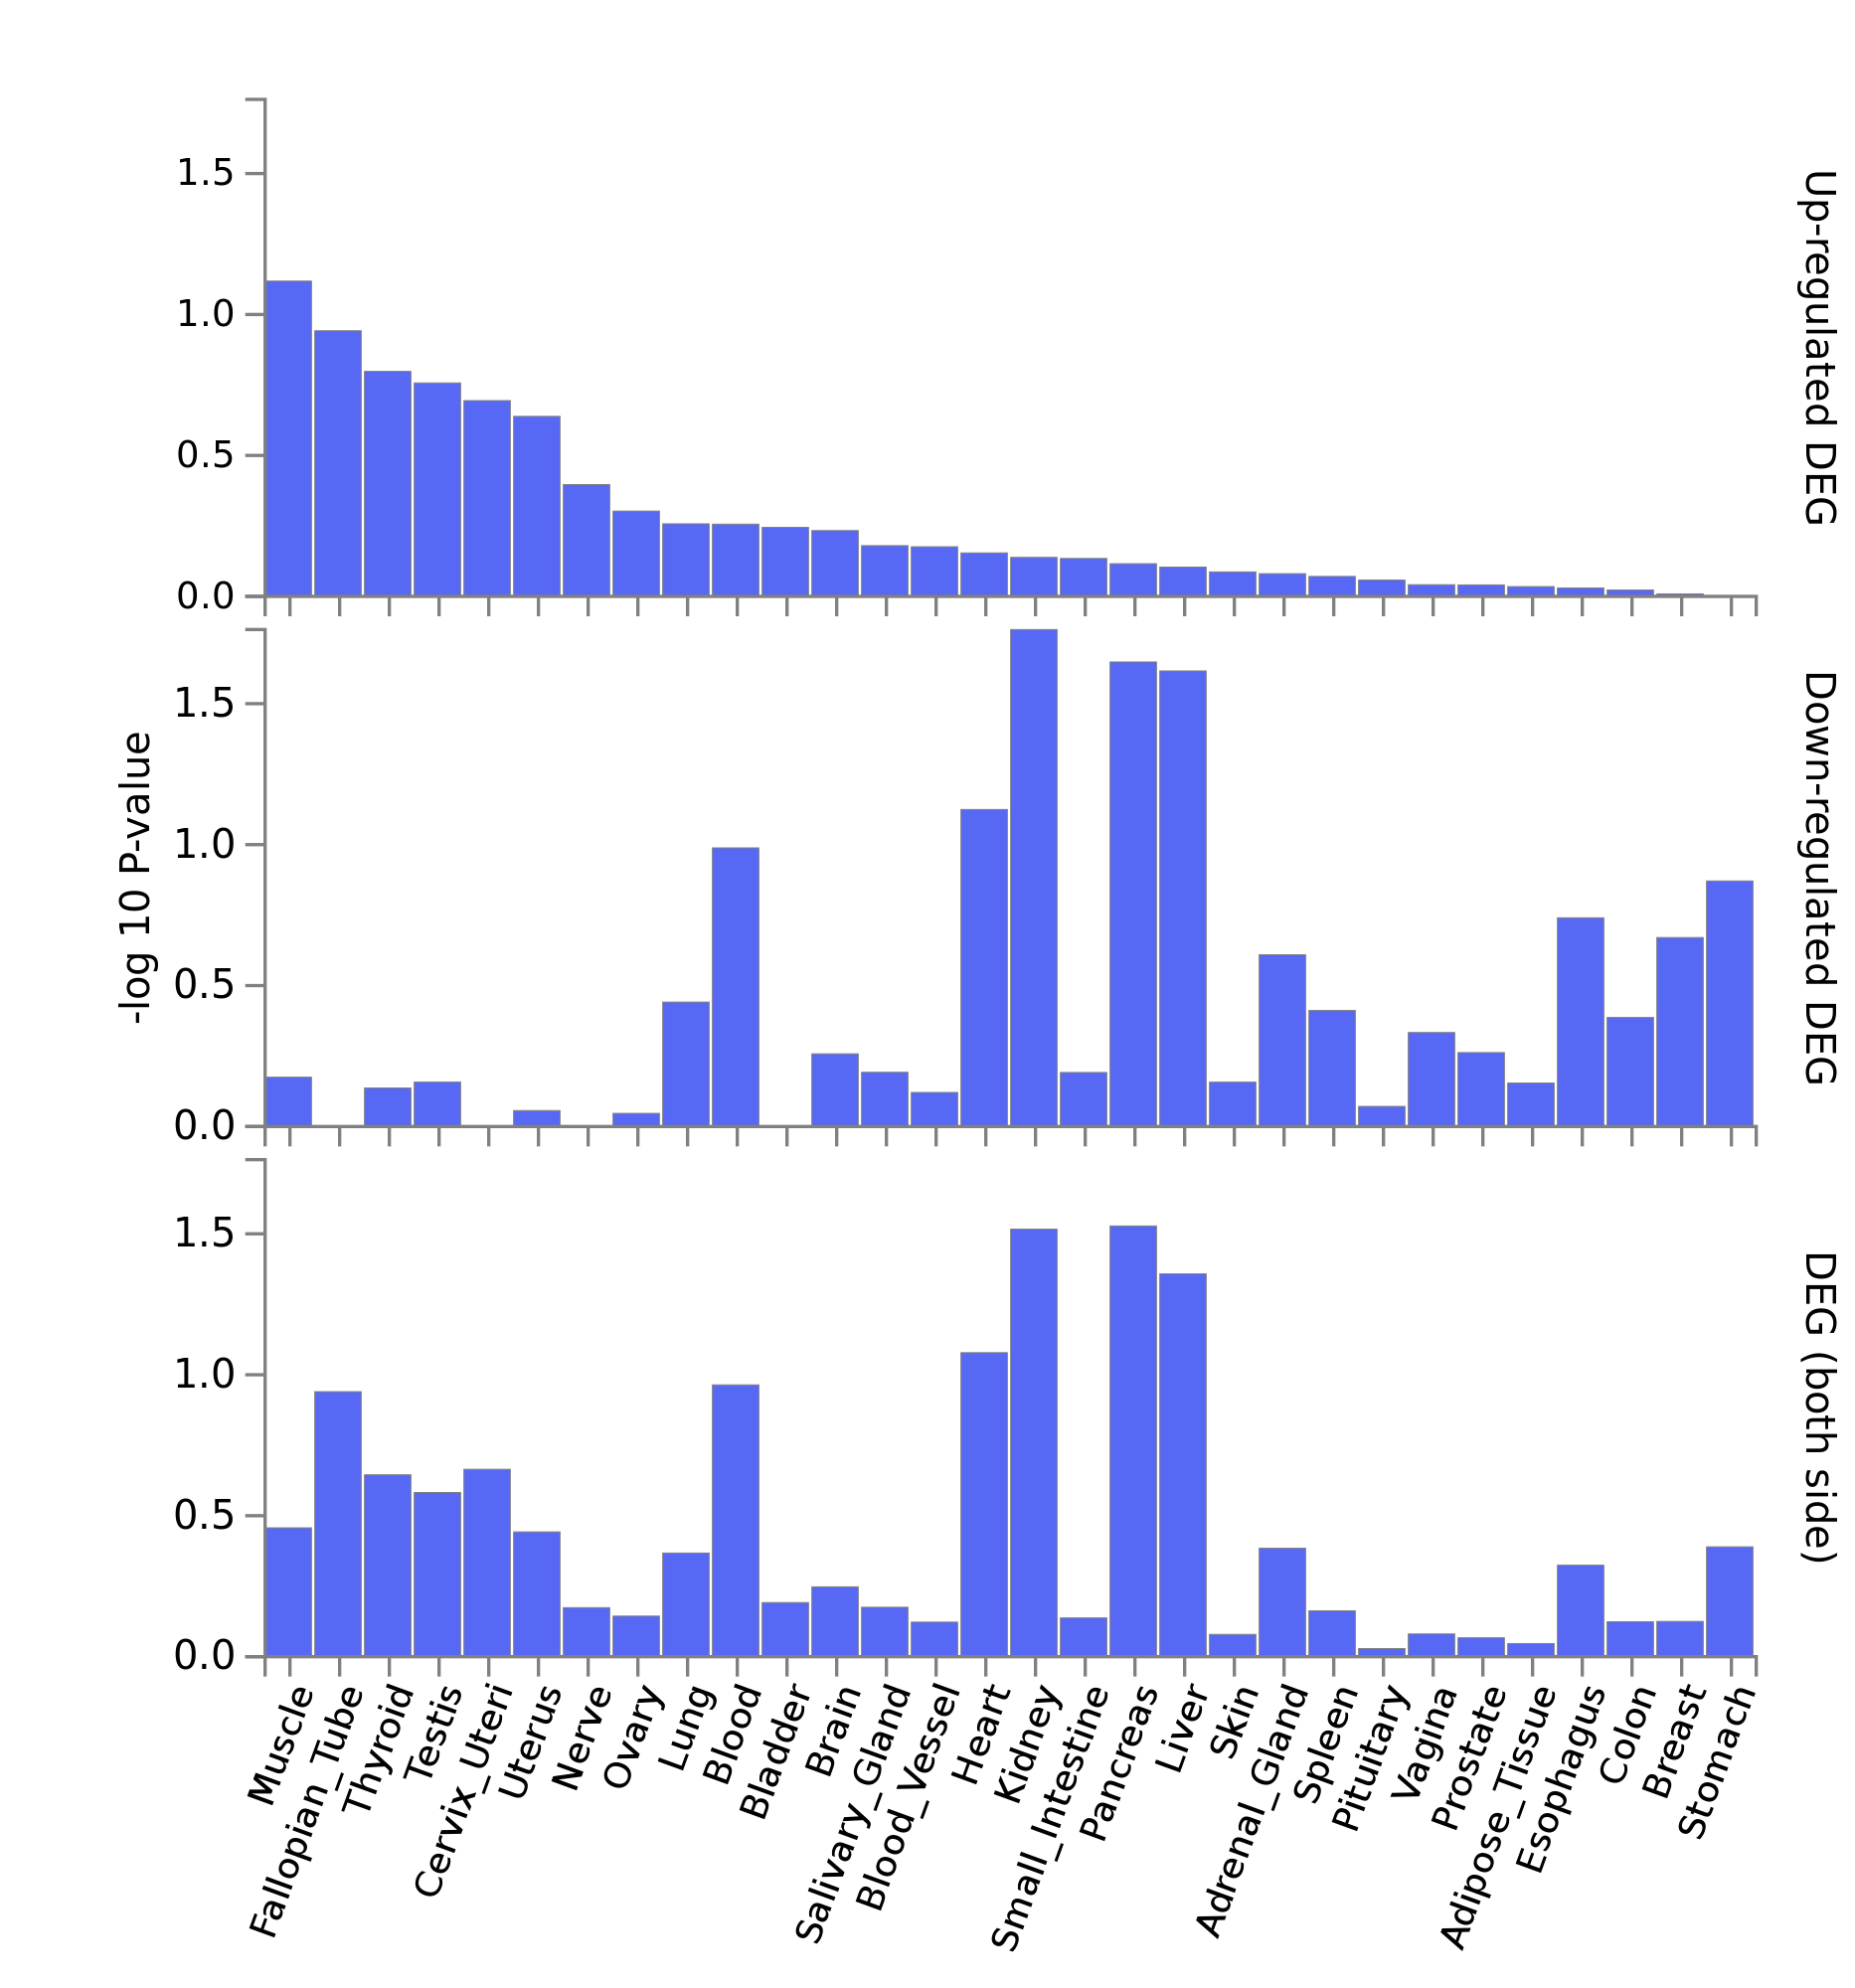
\includegraphics[width=7cm]{images/FUMA_plots/deg_general_up/ctg_upreg_general_gtex_v8_ts_general_FUMA_gene2func44709.png}
    \caption{Gene expression Intelligence Replication}
    \end{subfigure}
  \begin{subfigure}{8cm}
    \centering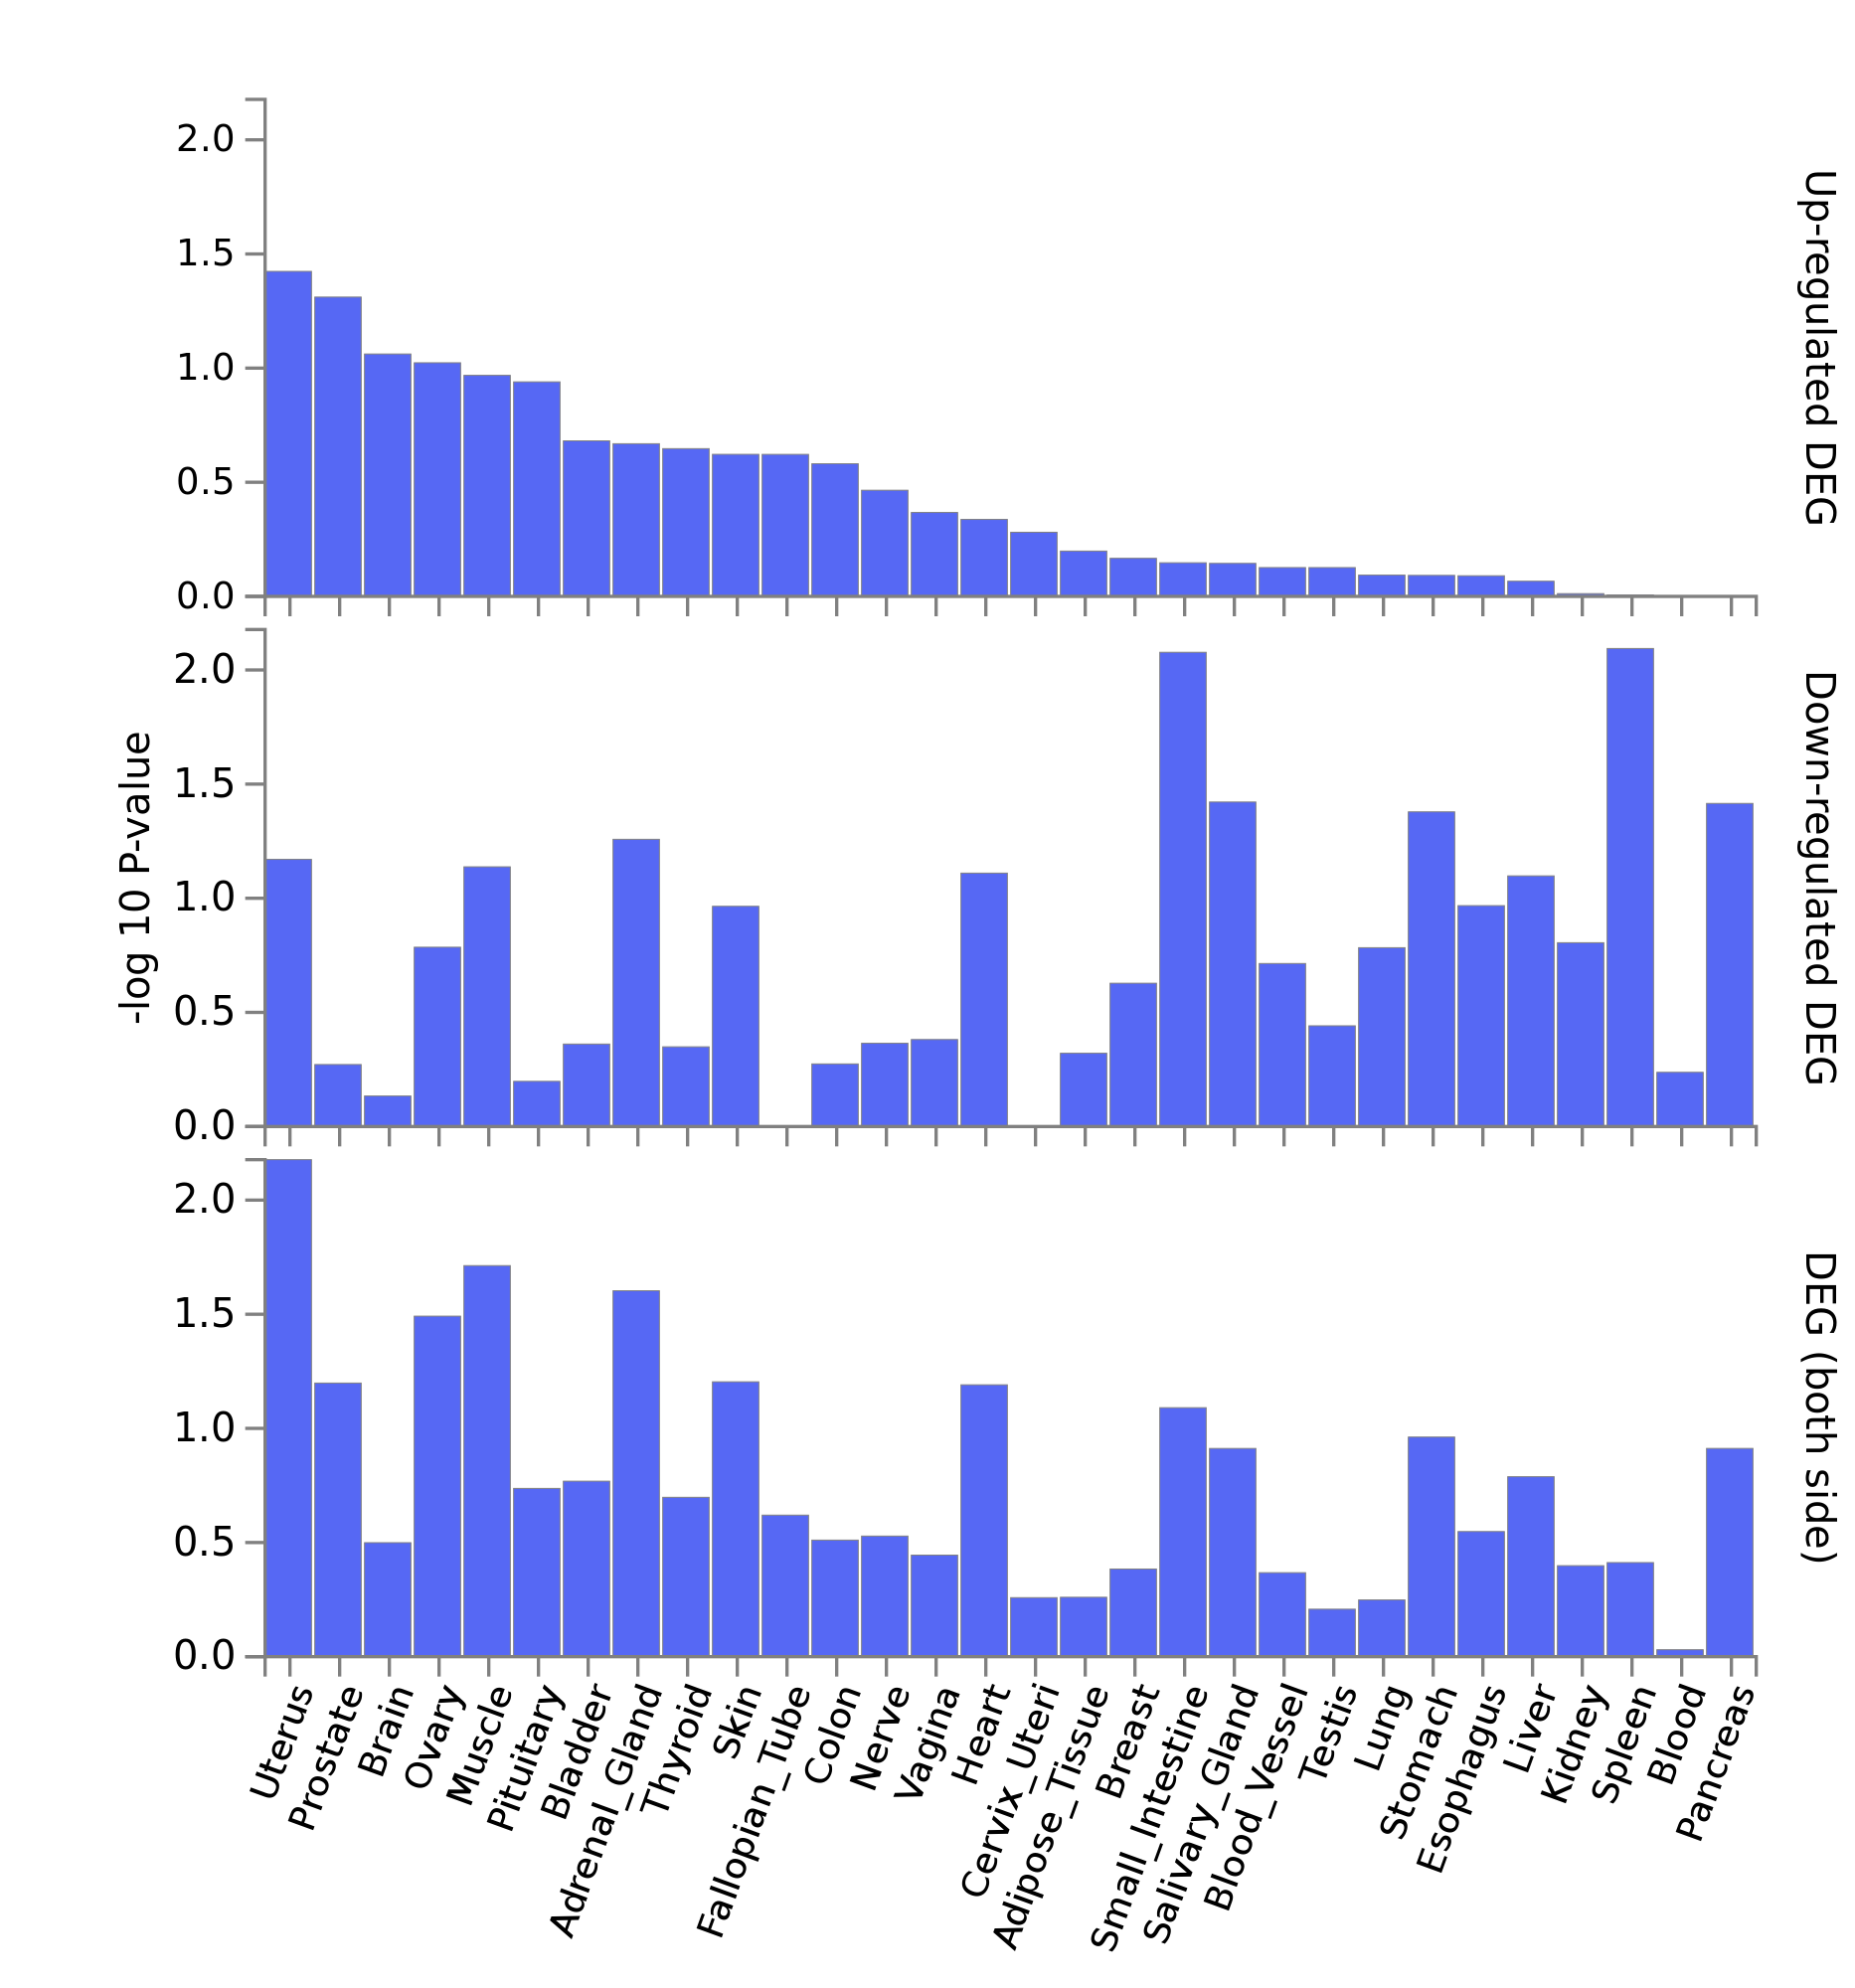
\includegraphics[width=7cm]{images/FUMA_plots/deg_general_up/ea2_corrected_upreg_general_gtex_v8_ts_general_FUMA_gene2func44667.png}
    \caption{Education Replication}
  \end{subfigure}
 
  \begin{subfigure}{8cm}
    \centering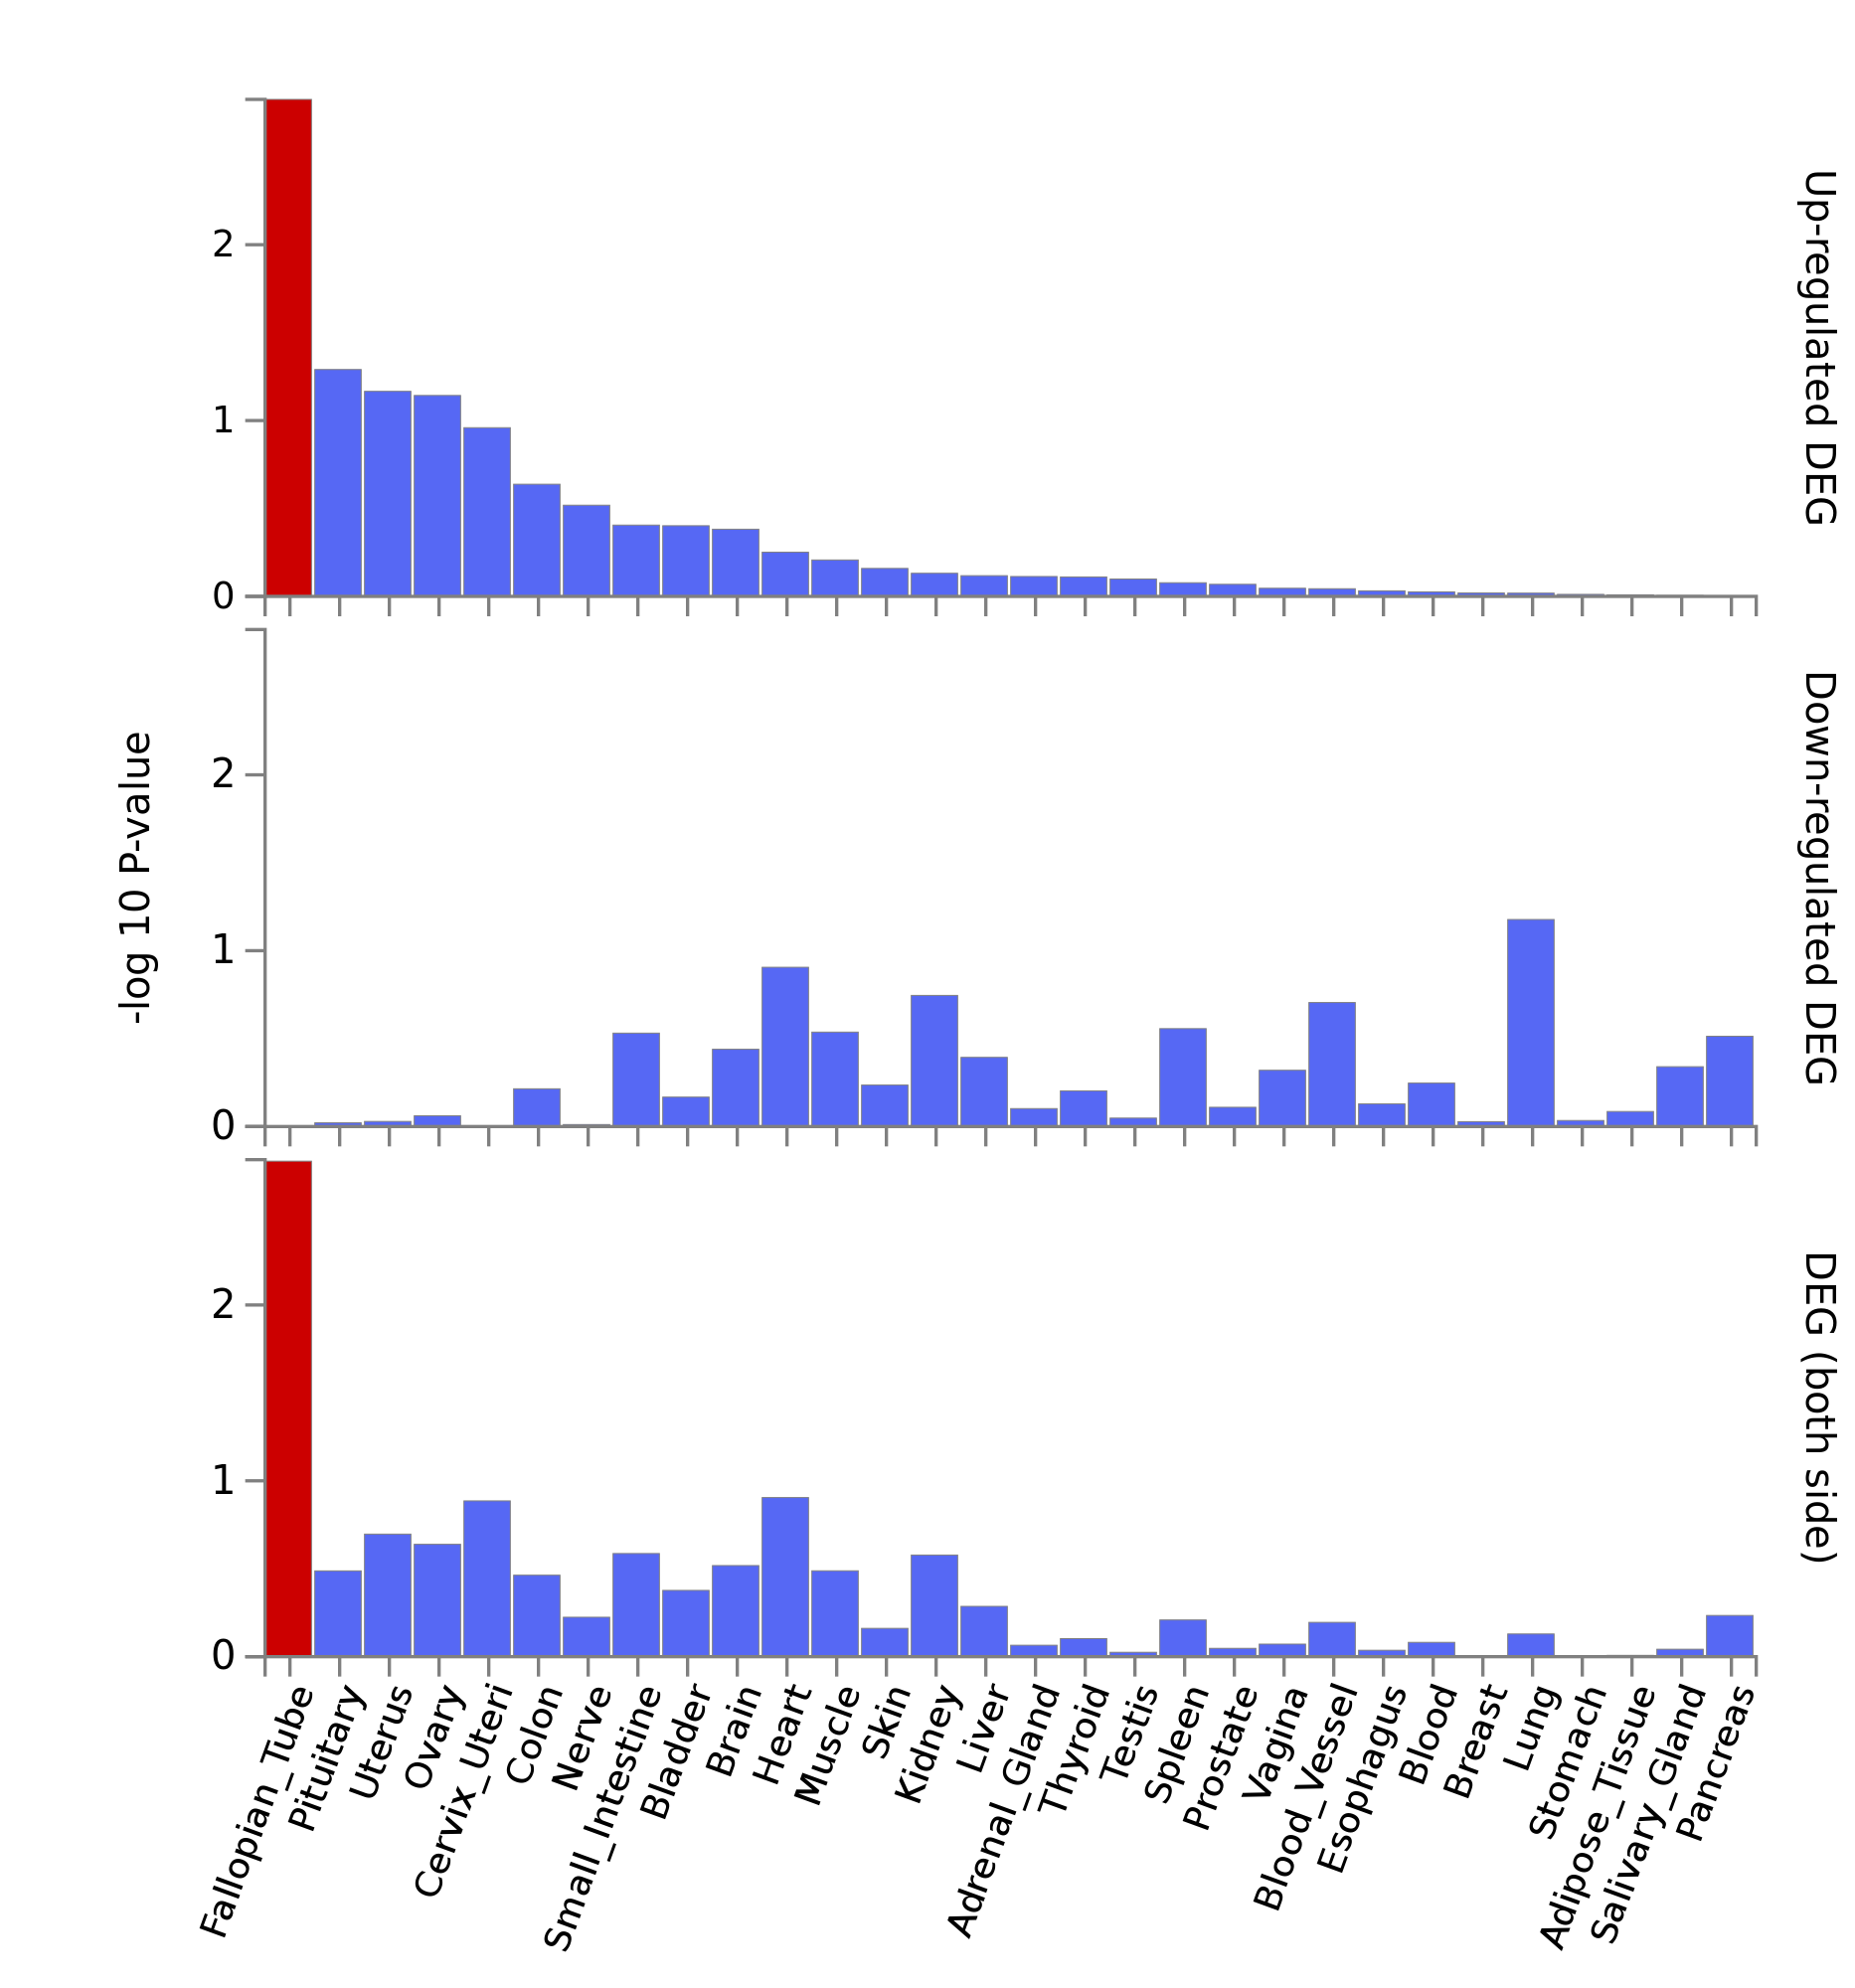
\includegraphics[width=7cm]{images/FUMA_plots/deg_general_up/ukbb_int_upreg_general_gtex_v8_ts_general_FUMA_gene2func44709.png}
    \caption{DEG Up Regulated Intelligence Discovery}
  \end{subfigure}
  \begin{subfigure}{8cm}
    \centering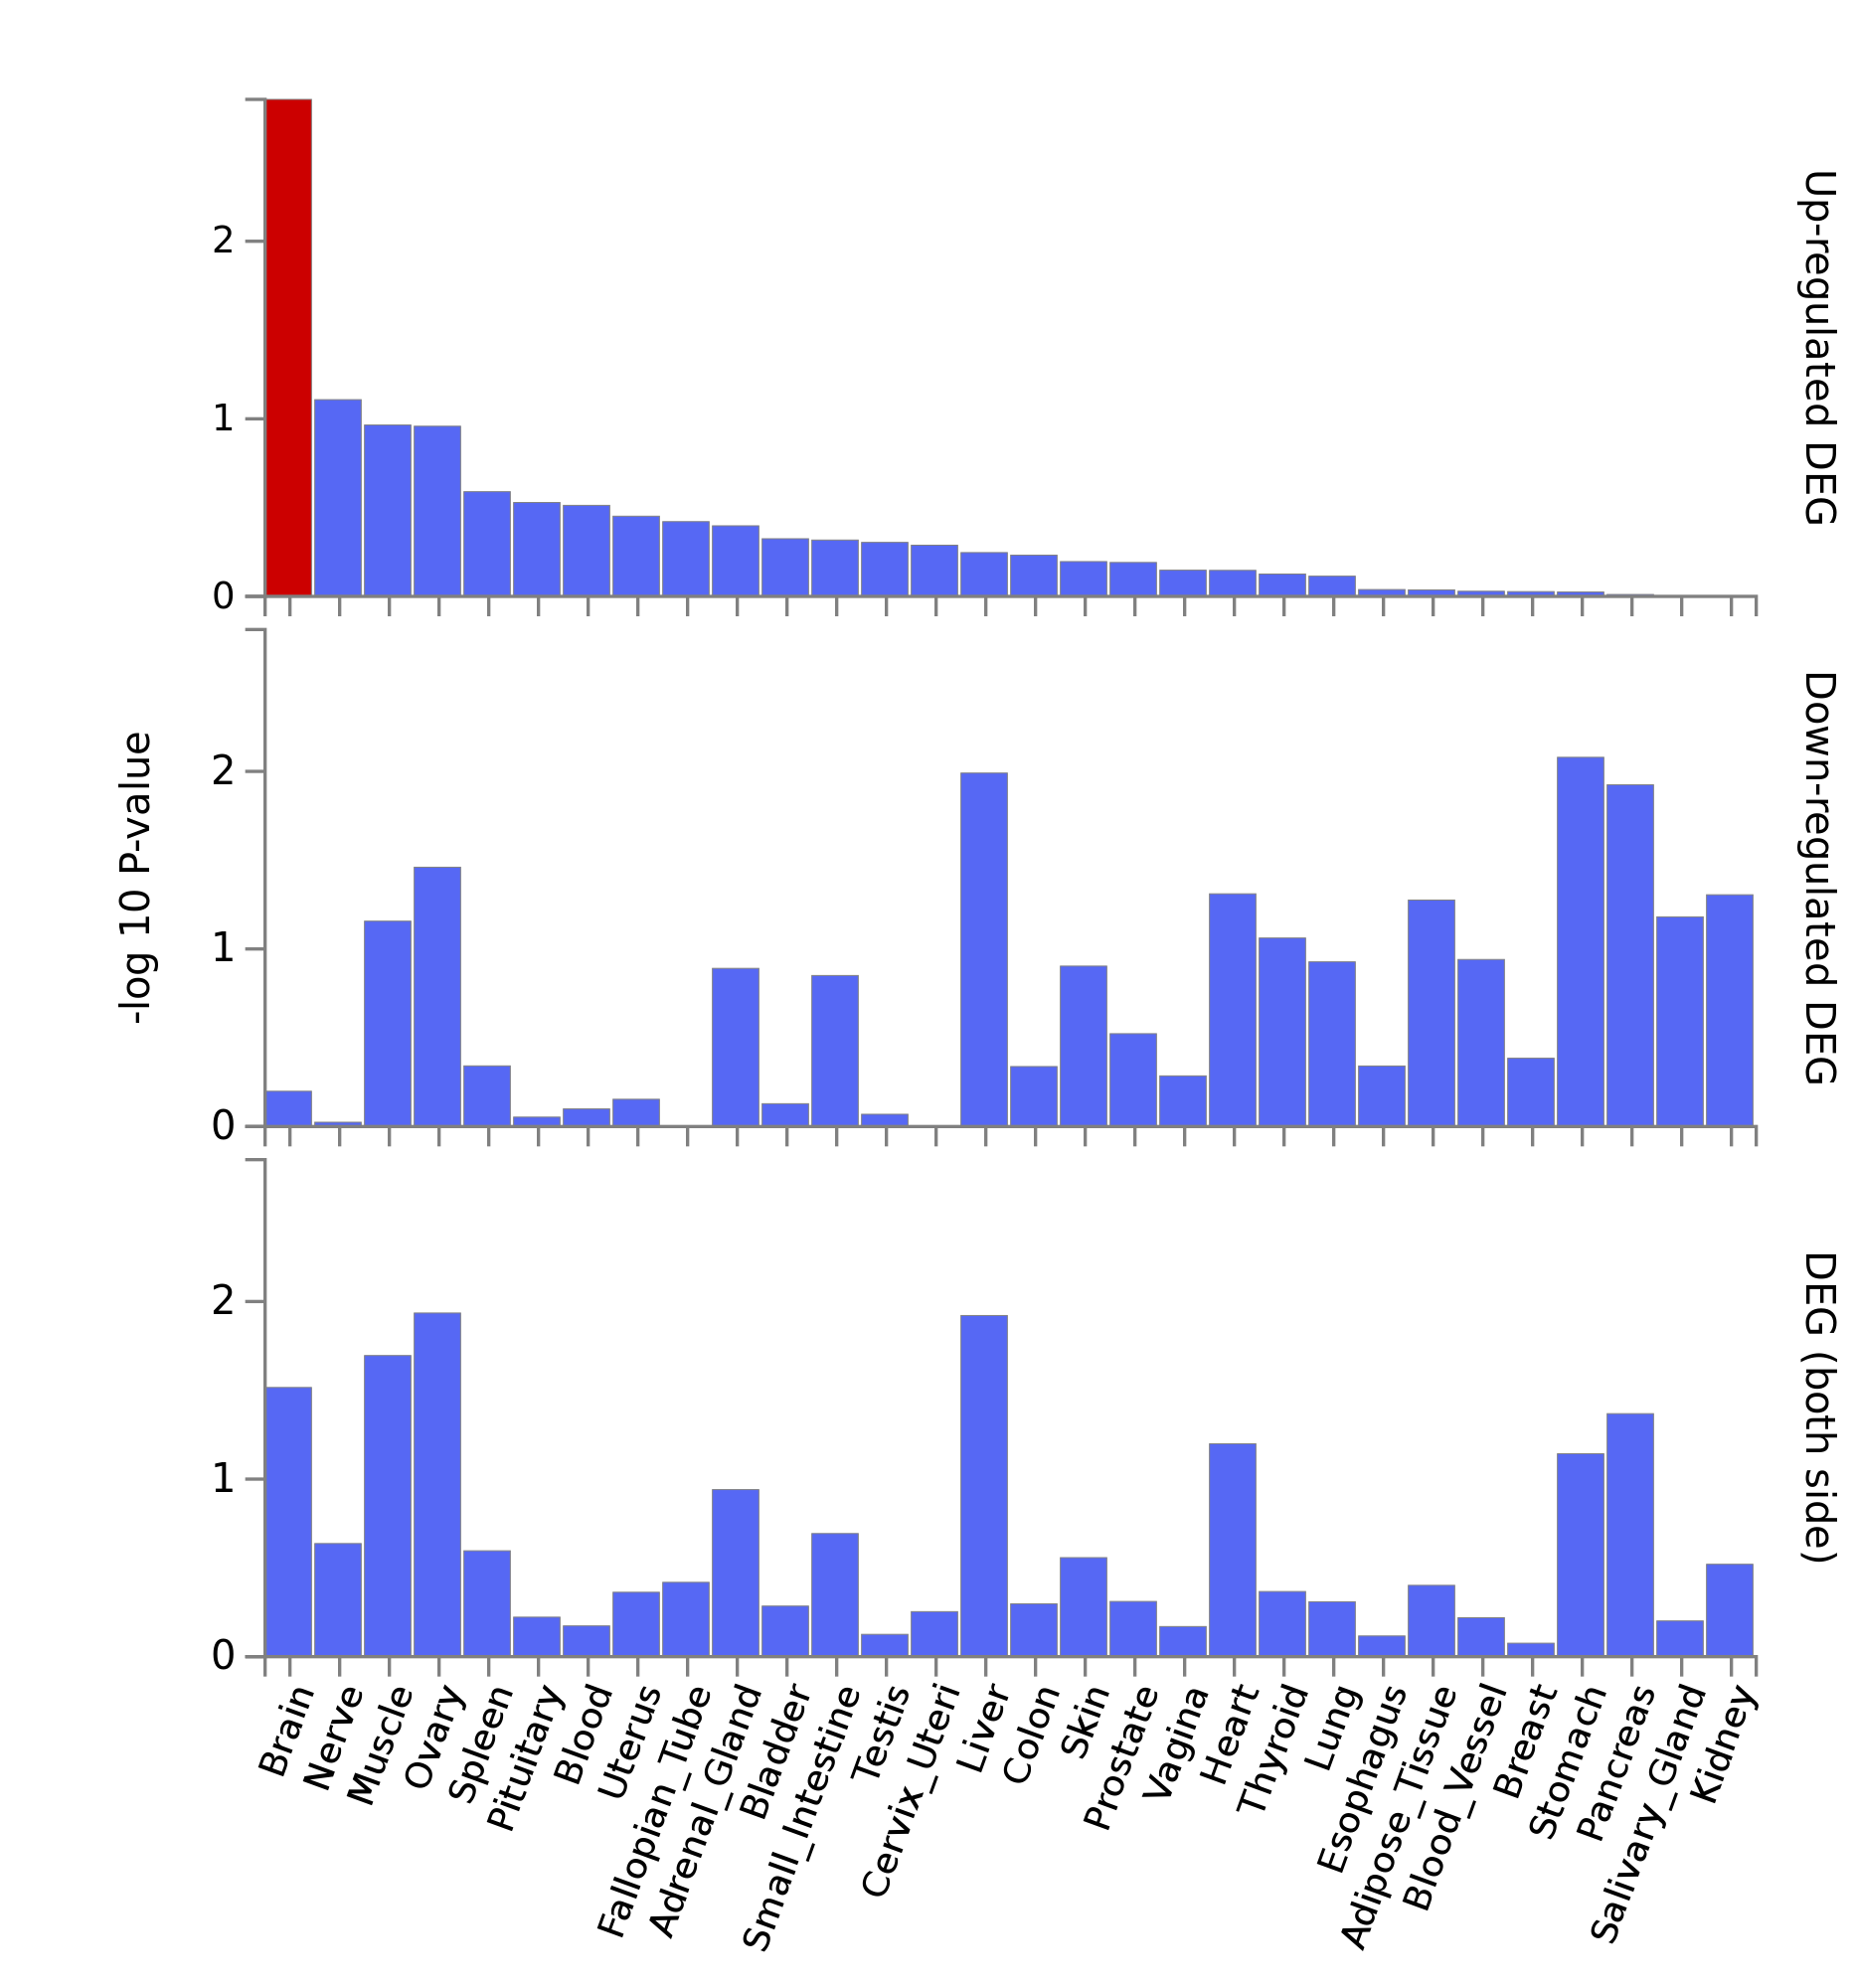
\includegraphics[width=7cm]{images/FUMA_plots/deg_general_up/ukbbed_upreg_general_gtex_v8_ts_general_FUMA_gene2func44709.png}
    \caption{Education Discovery}
  \end{subfigure}
  \caption{FUMA output. Enrichment for differentially expressed genes ordered by up regulated genes. Only education discovery shows evidence of up regulated differentially expressed genes in CNS}
  \label{fig:FUMA gtex deg samples multiple}
\end{figure}

 \begin{figure}
  \begin{subfigure}{8cm}
    \centering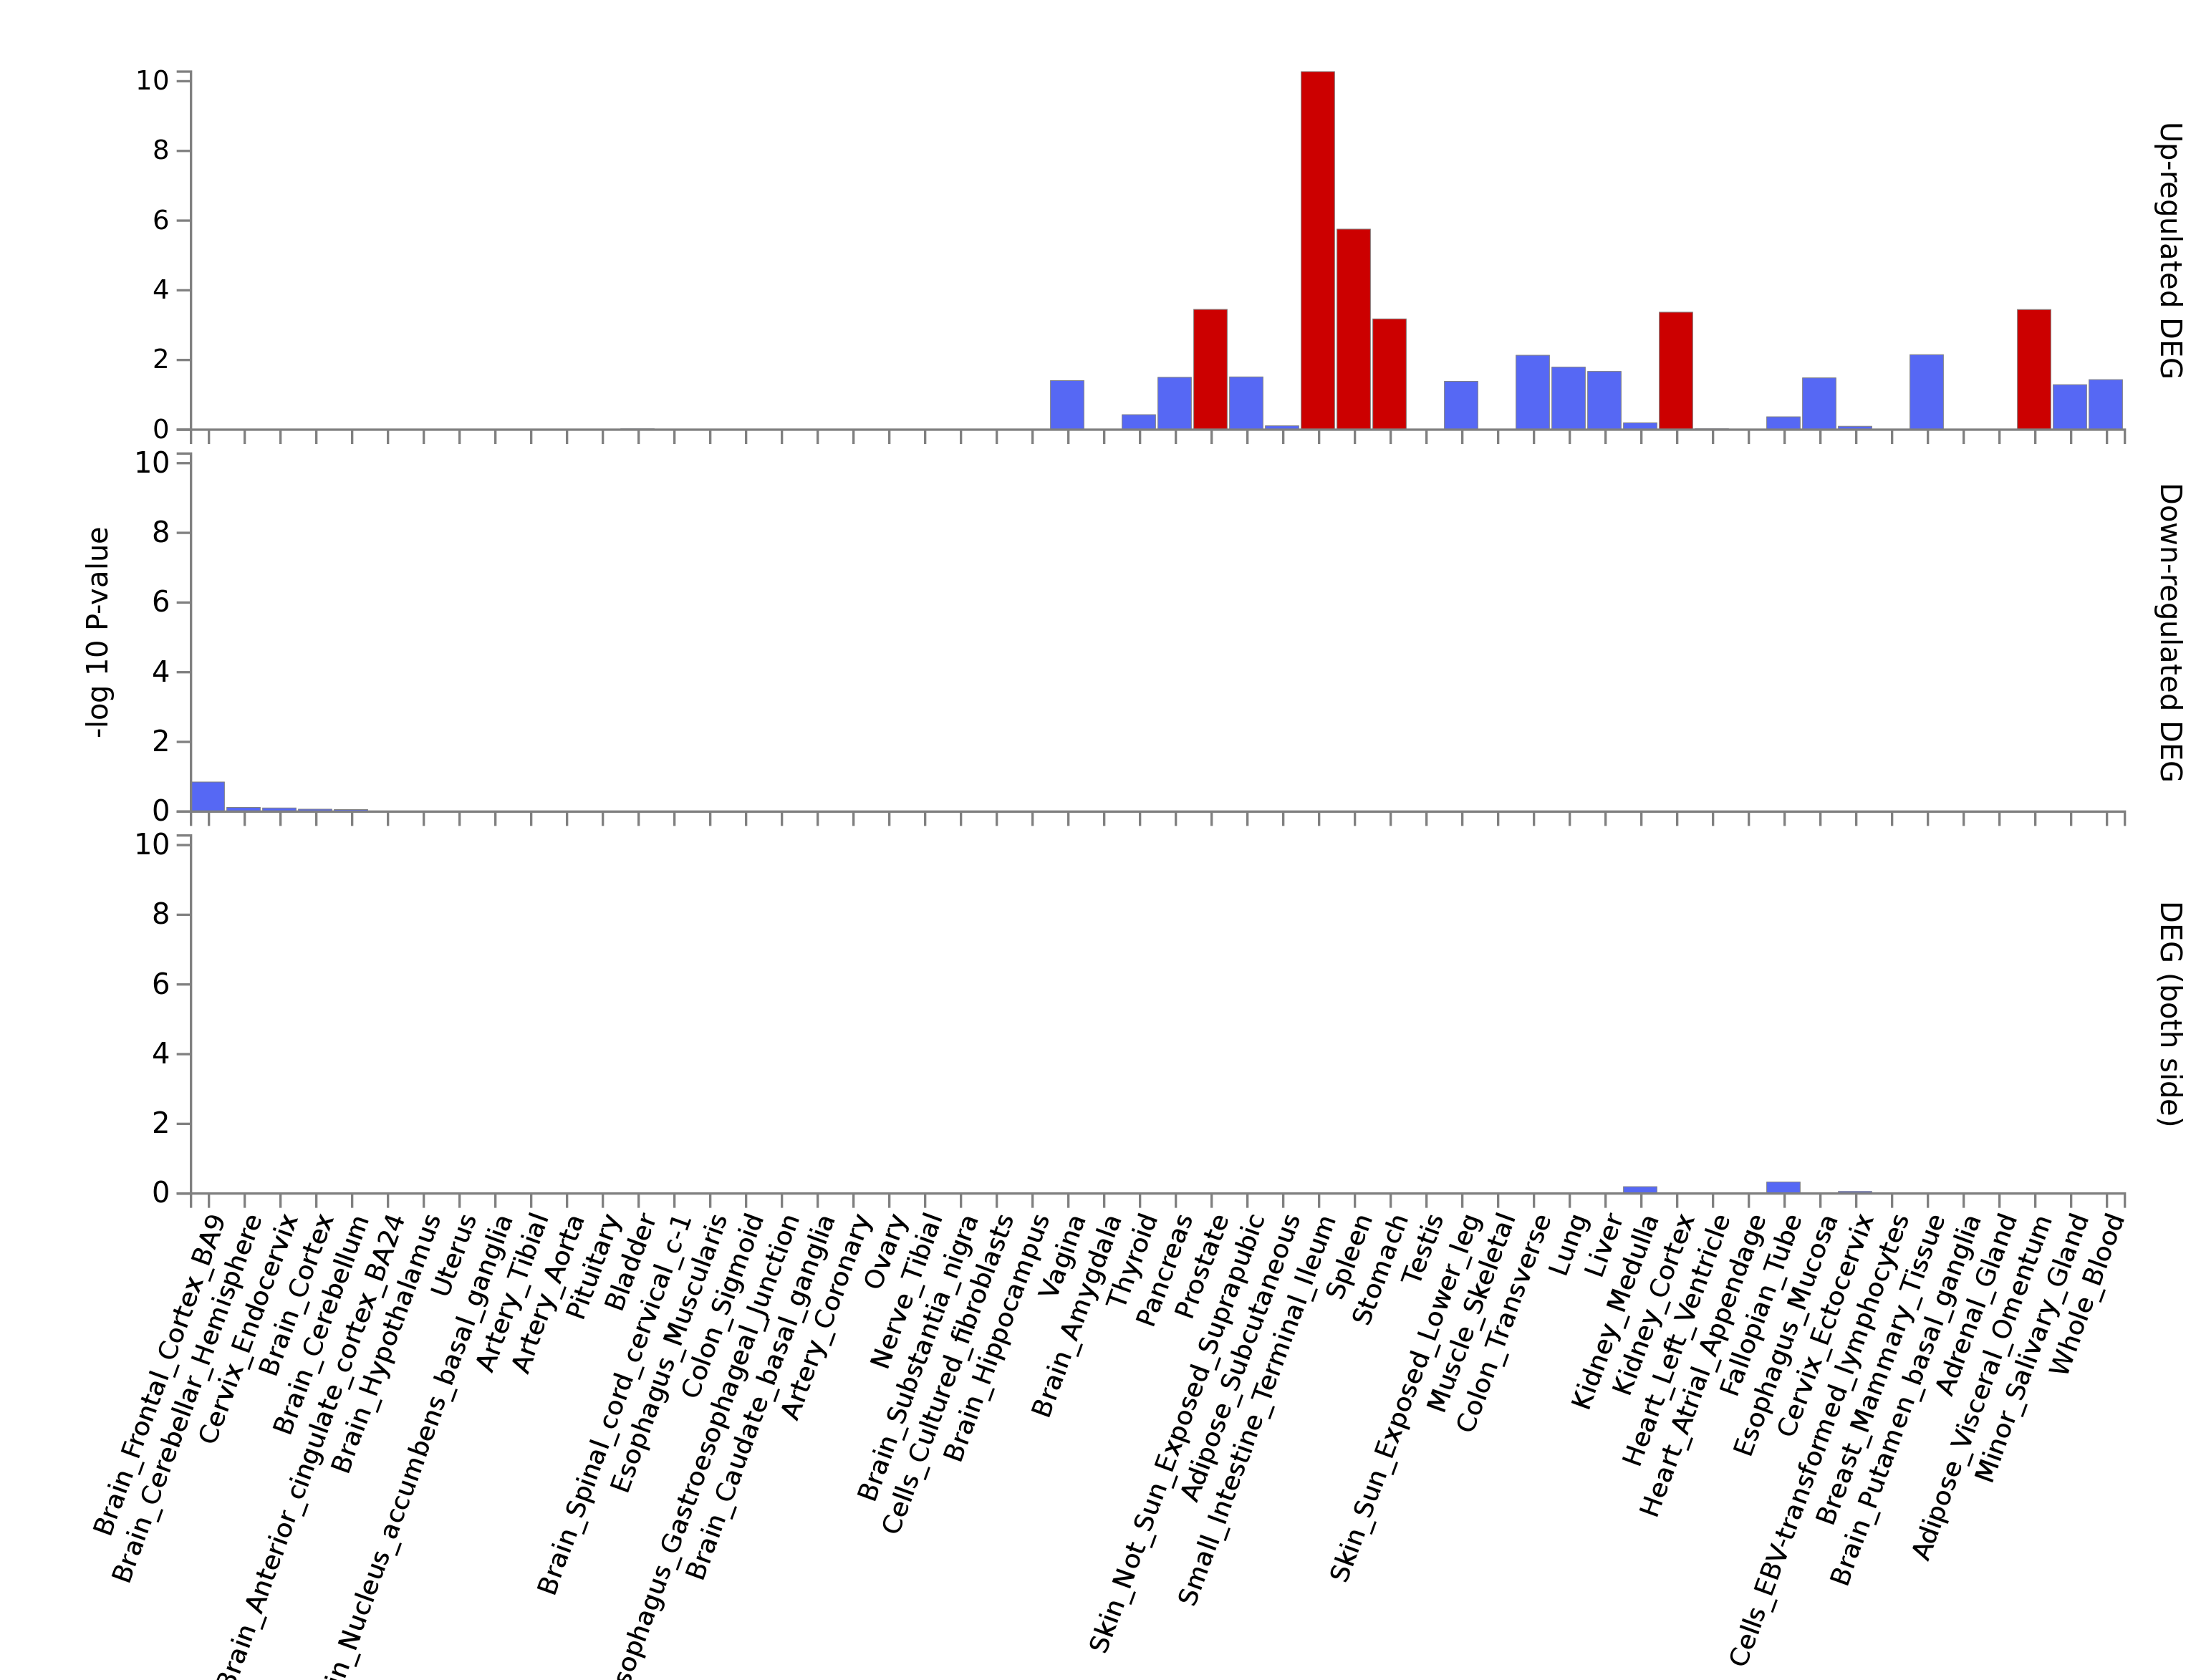
\includegraphics[width=7cm]{images/FUMA_plots/gtex_v8_ts_nonPSP_FUMA_gene2func44651.png}
    \caption{Gene expression genes not in PSP}
    \end{subfigure}
  \begin{subfigure}{8cm}
    \centering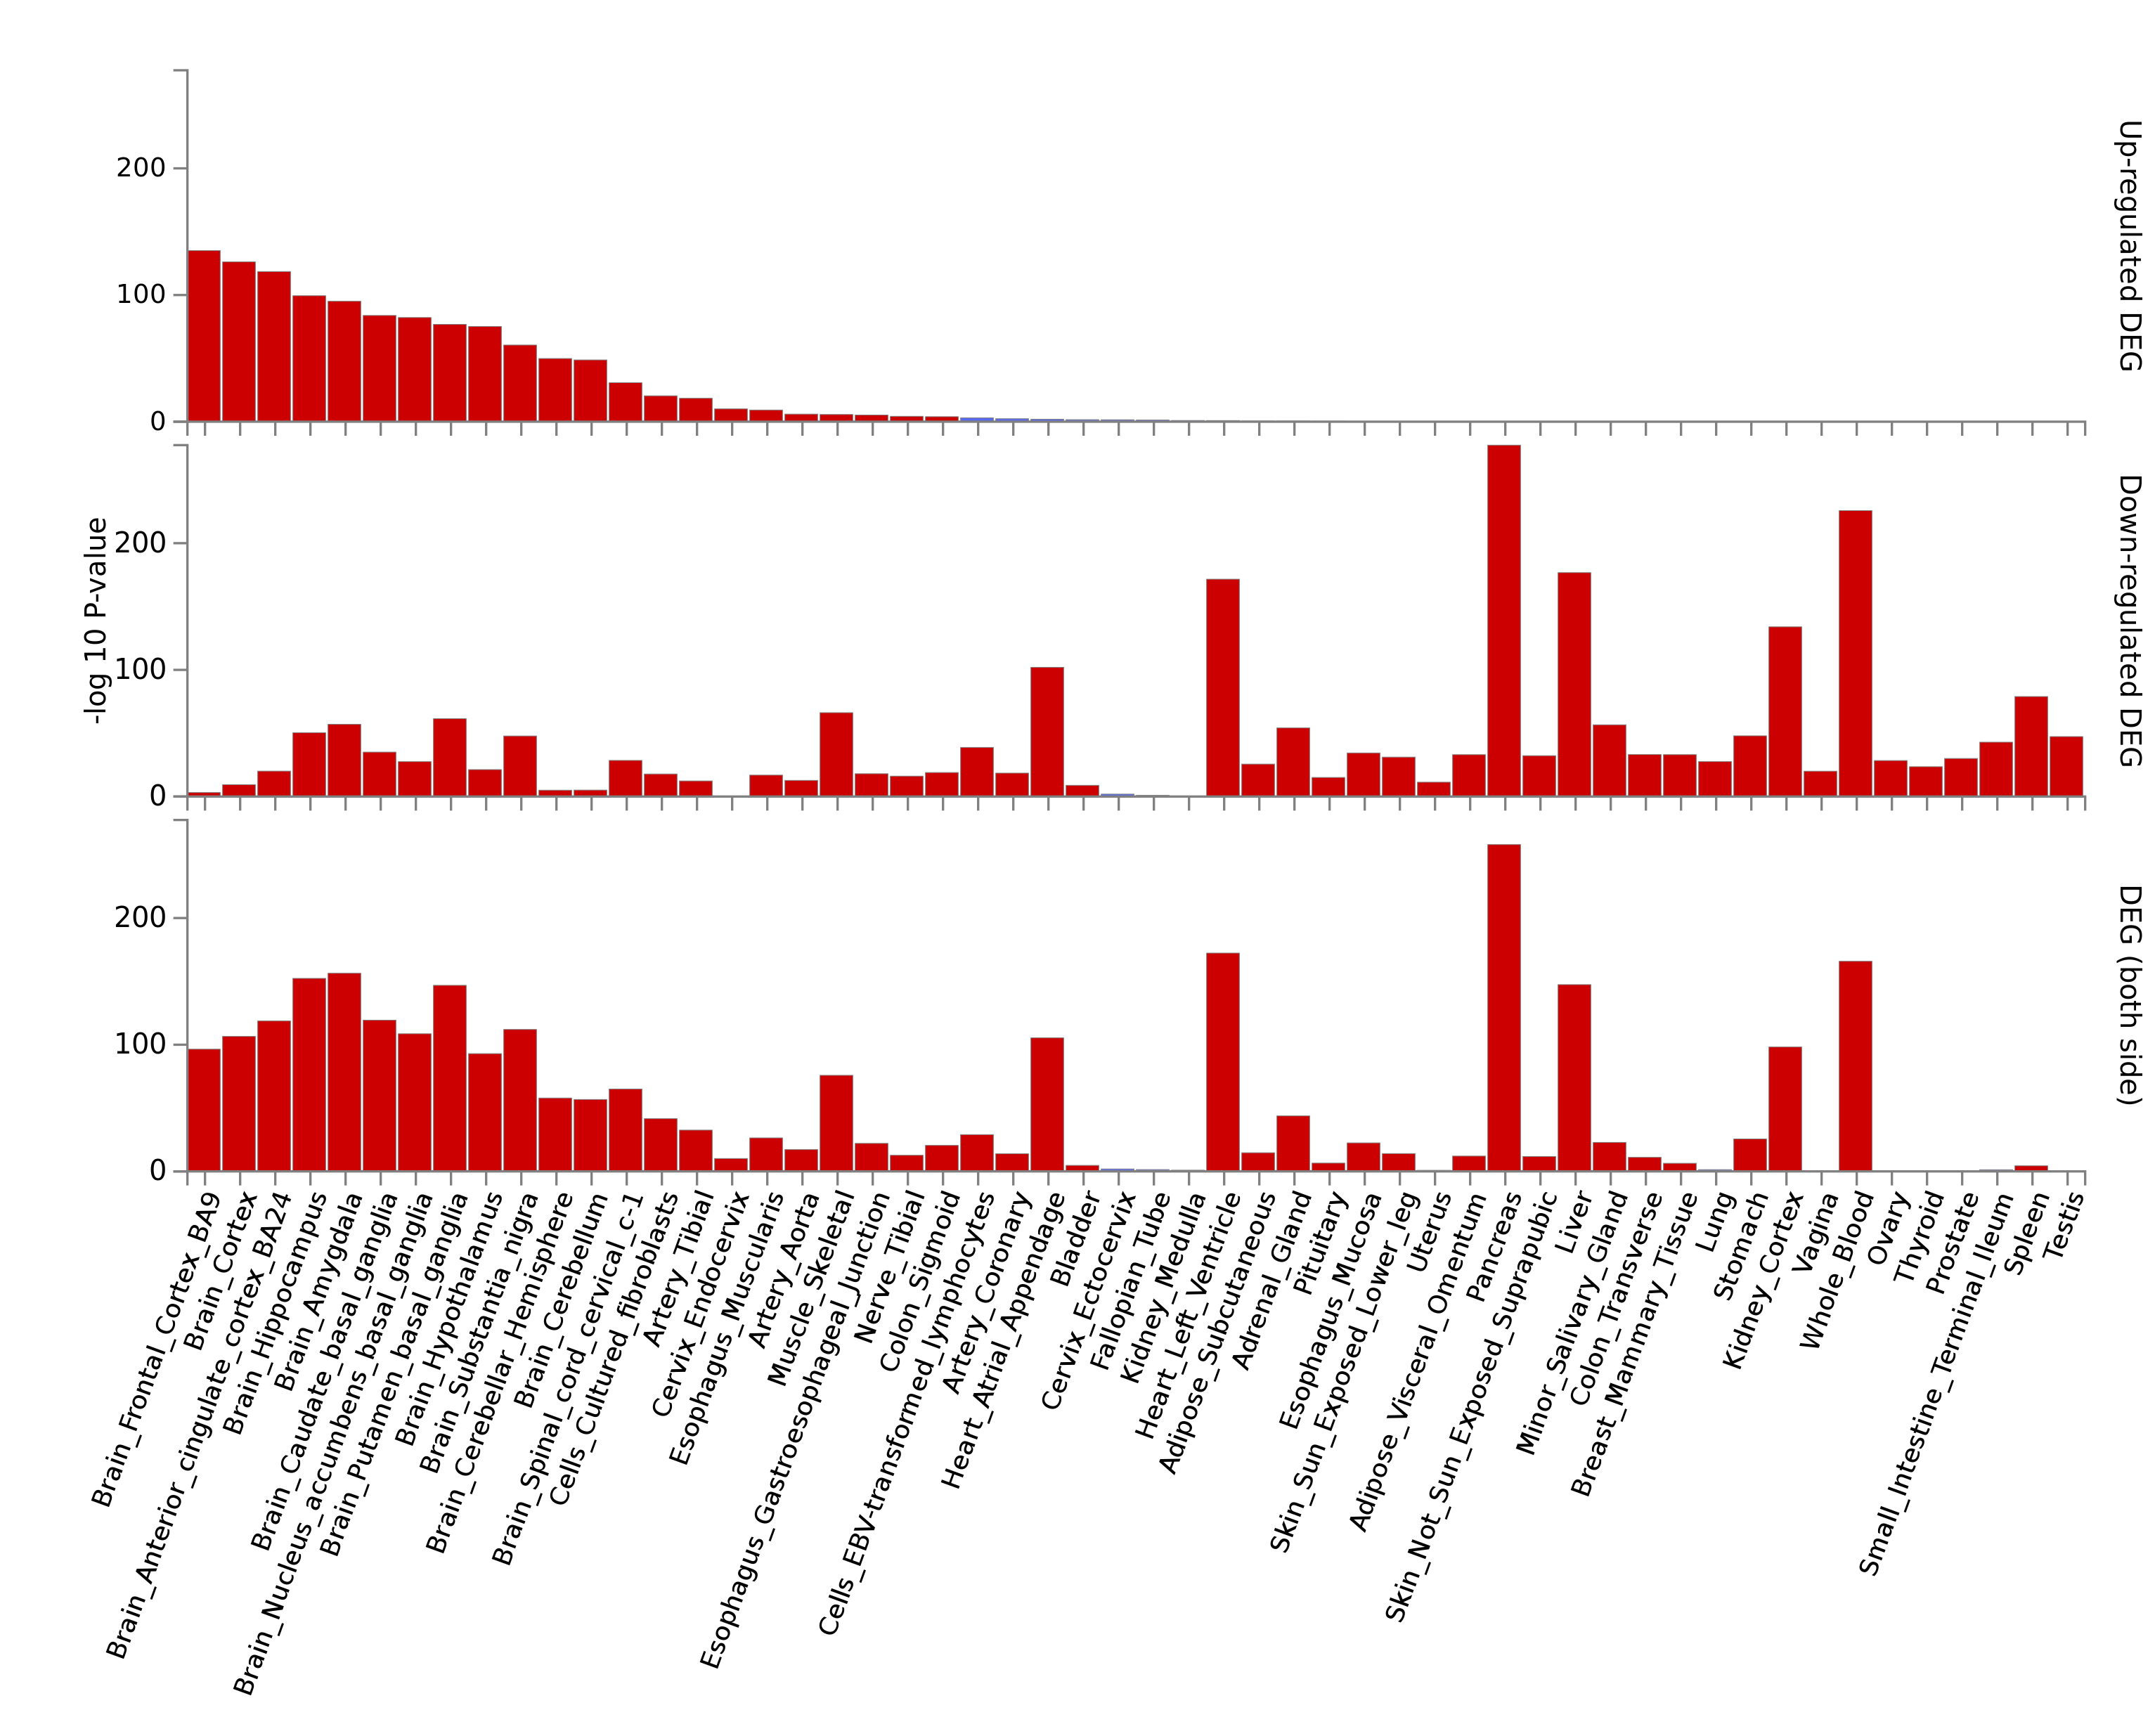
\includegraphics[width=7cm]{images/FUMA_plots/gtex_v8_ts_FUMA_PSP_gtex.png}
    \caption{Genes in PSP}
  \end{subfigure}
 
  \begin{subfigure}{8cm}
    \centering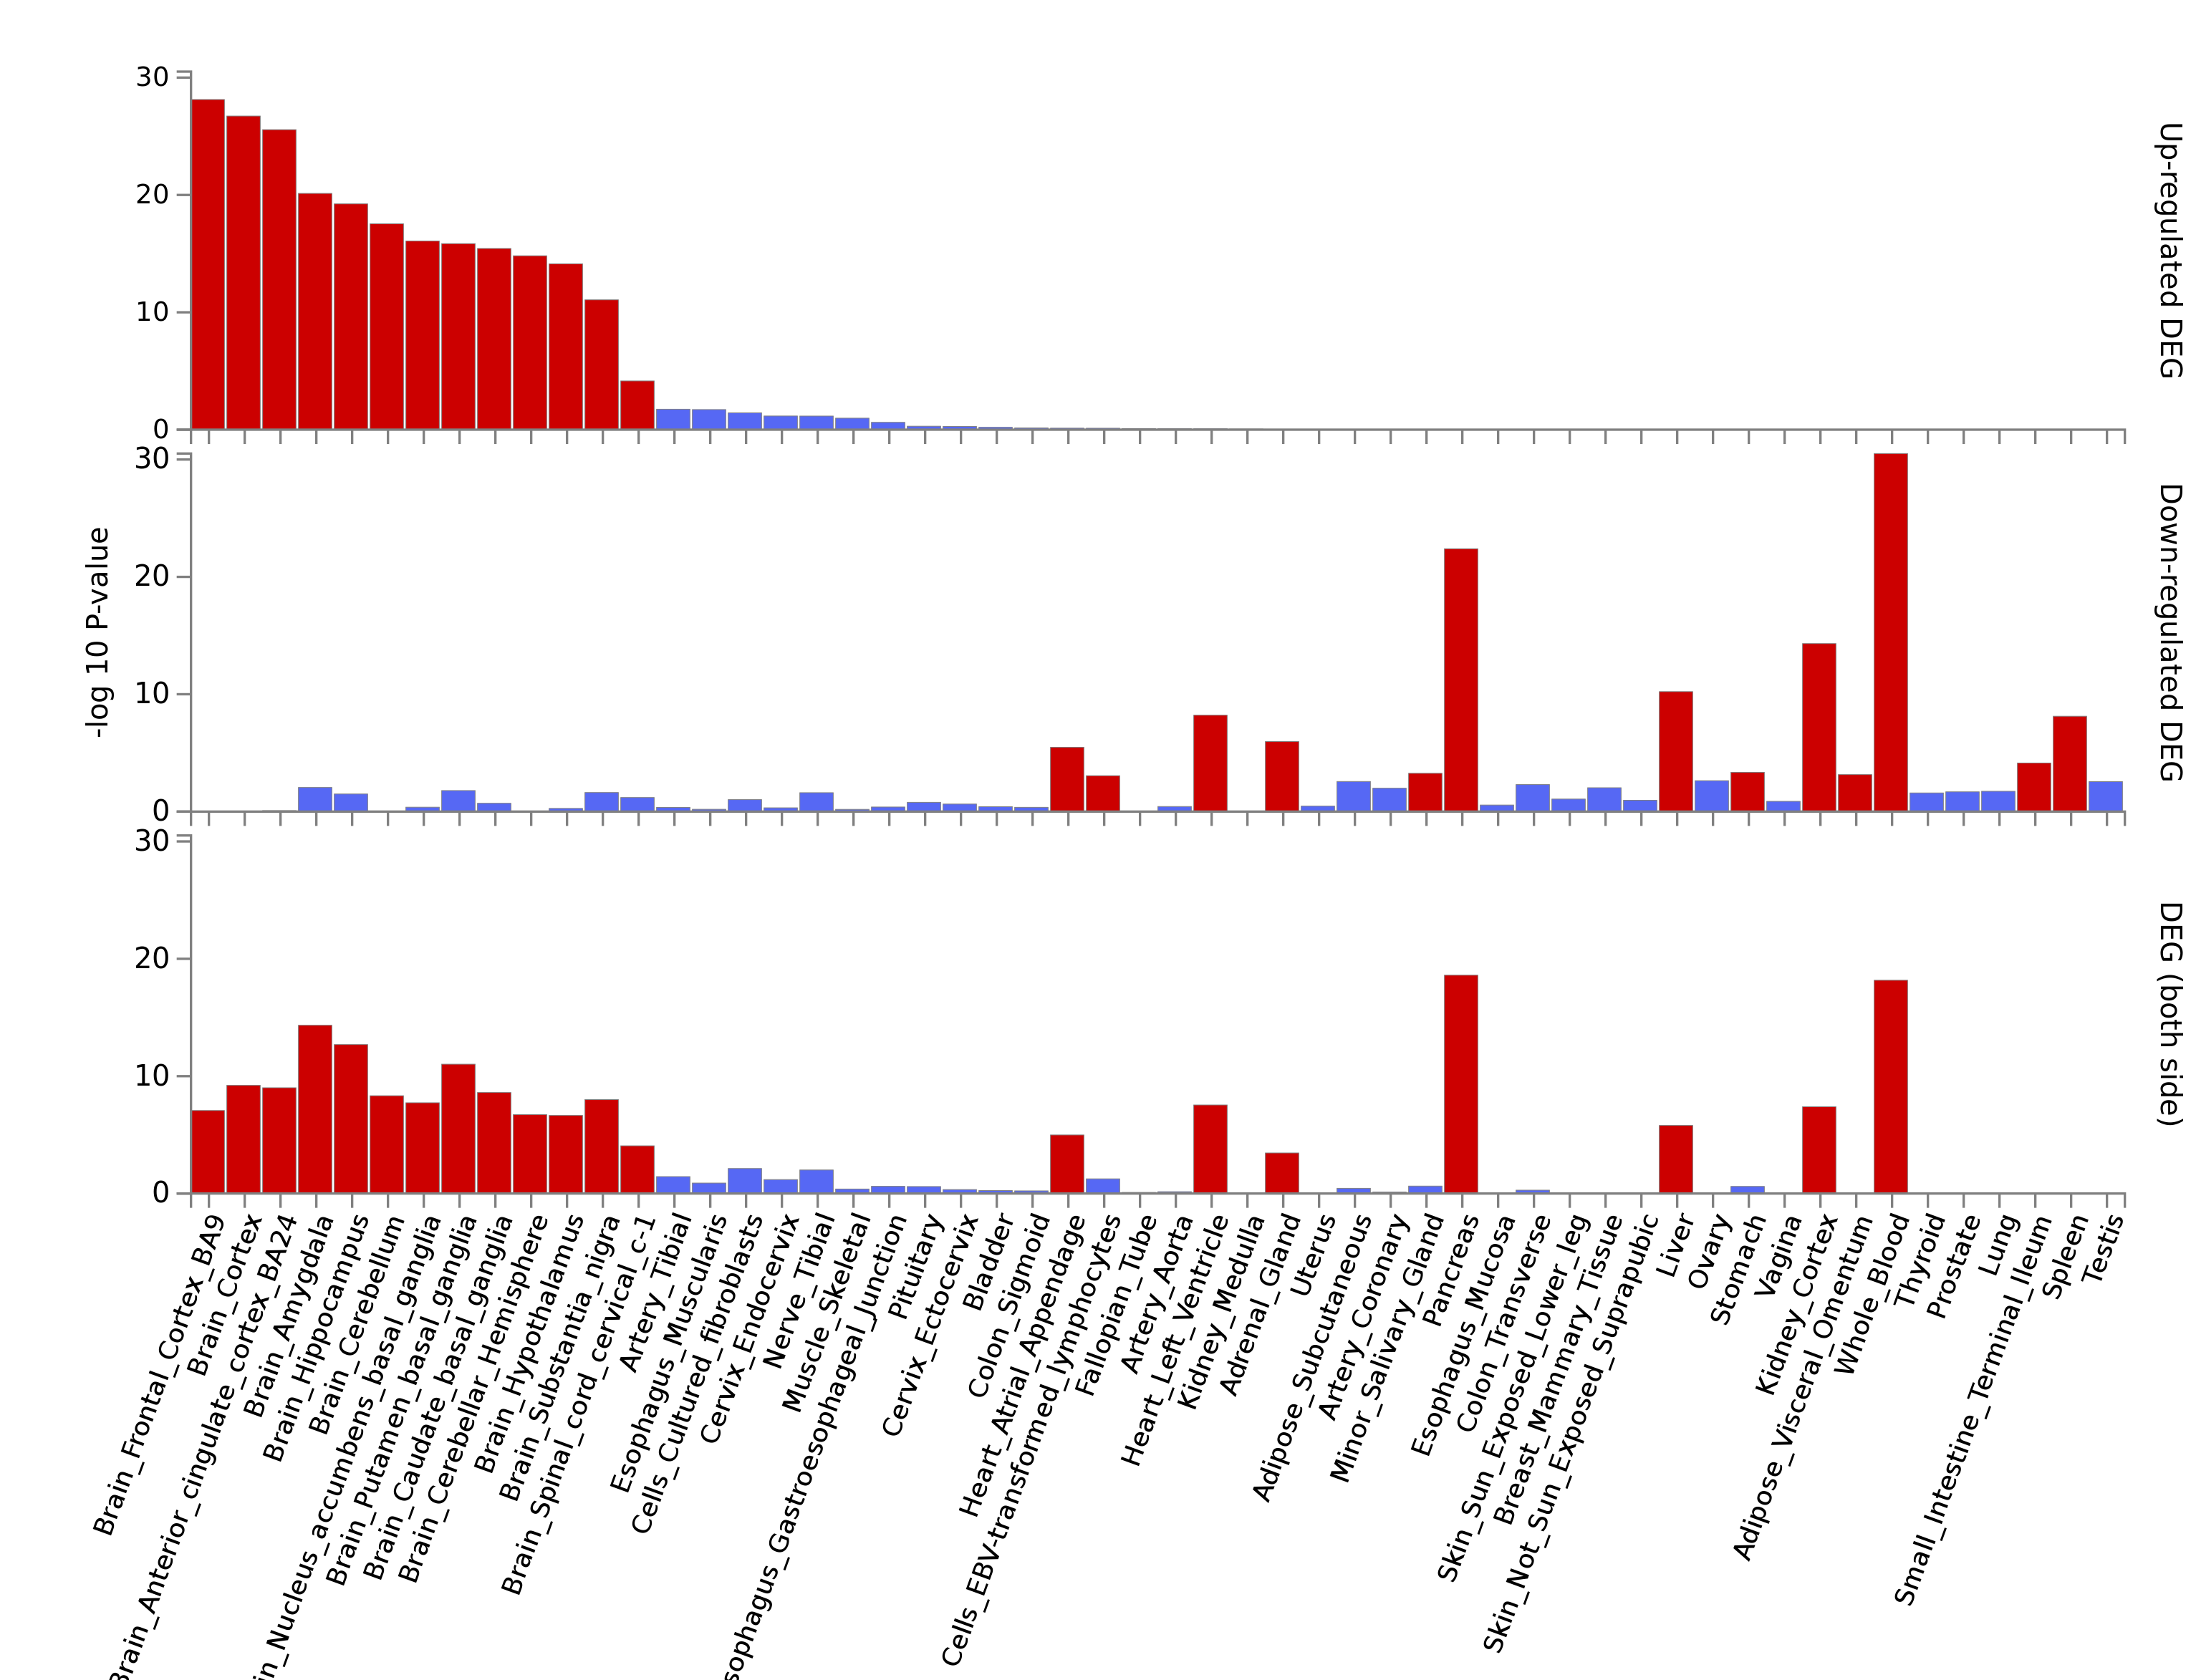
\includegraphics[width=7cm]{images/FUMA_plots/gtex_v8_ts_psp_not_consensus_FUMA_gene2func44650.png}
    \caption{Genes in PSP but not in consensus PSD. ie new genes}
  \end{subfigure}
  \begin{subfigure}{8cm}
    \centering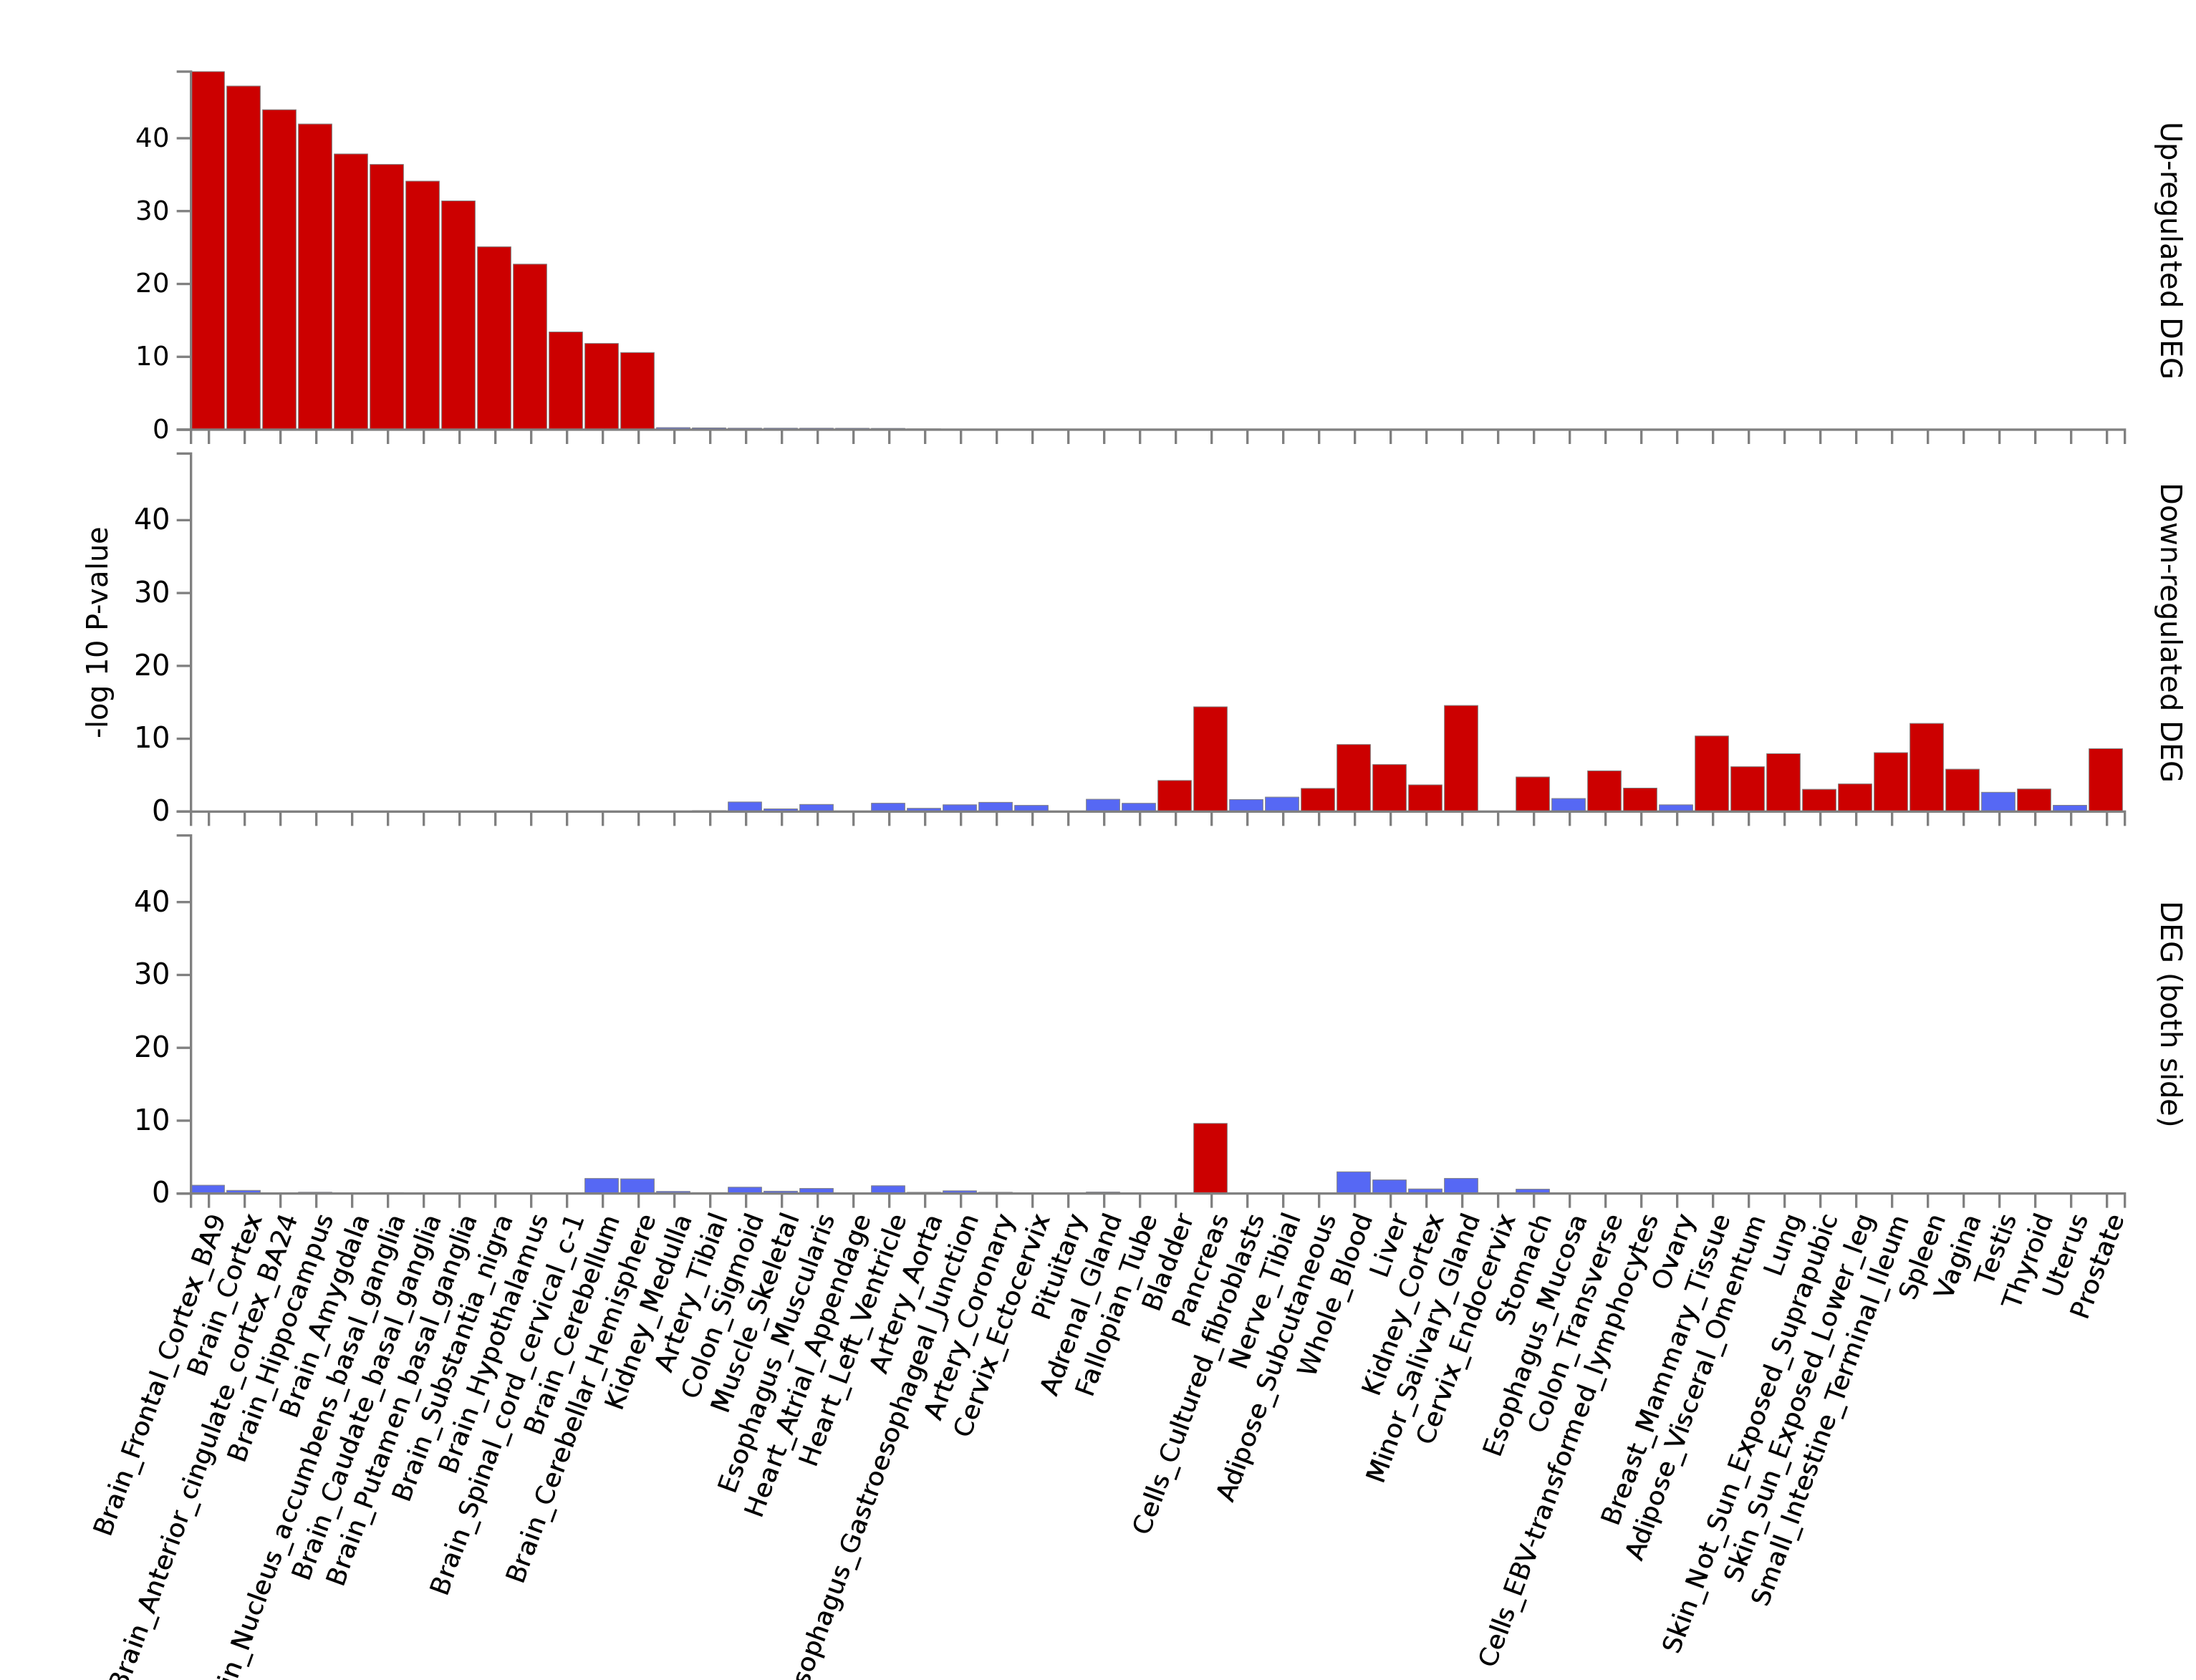
\includegraphics[width=7cm]{images/FUMA_plots/gtex_v8_ts_1313_consensus_FUMA_gene2func44650.png}
    \caption{Genes in consensus PSD}
  \end{subfigure}
  \caption[\textbf{Comparison of gene expression} in consensus PSD and PSP]{Comparison of gene expression in genes not in the PSP, genes in the PSP, genes in PSP but not in the consensus PSD (new genes), genes in the consensus PSD - that which is conserved in different vertebrate species. Images from FUMA. GTEx v8 54 tissue types. Ordered from left to right by up-regulated differentially expressed genes p values (hypergeometric test). Tissues with significant differential enrichment after bonferroni correction for multiple comparisons are shown in blue. Y axis -log10(p) of enrichment for gene set (eg PSP) }
  \label{fig:compare all PSP gtex multipanel FUMA output}
\end{figure}

 
 

%%%%%%%%%%%%%%%%%%%%%%%%%%%%%%%%%%%%%%%%%%%%%%%%%%%%%%%%%%%%%%%%%%%%





\clearpage
\section{Synaptic component enrichment MAGMA}
\label{Synaptic component enrichment MAGMA}

Functional synaptic group gene sets are curated  at the Complex Trait Genetics lab \footnote{\url{https://ctg.cncr.nl/software/GENESETS/synapse.zip}} based on stuies by Ruano et al. (2012)\cite{ruano2010functional}\footnote{paper looking at G protein receptors} and Lips et al. (2012)\cite{lips2012functional}. Using these sets with MAGMA will provide an estimate of how effective a purely functional annotation approach is and an estimate of the value of significance tests in these samples. 

MAGMA GSA was performed using the raw output of the GWGAS analyses in MAGMA as part of a standard two stage MAGMA GSA. Default options were used.
The annotated set was composed of 1028 genes. 736 of these were in the PSP, 292 were not. A large number of the missing ones were non glutamatergic receptors and the  proteins associated with these. There are 18 gene sets each a functional group such as G-protein-coupled receptor signalling.

MAGMA accepts gene sets in gene matrix transposed format (gmt) where each gene set is a row in a text file that is tab separated. gmt files used for MAGMA enrichment are often those curated by MSigDB. I have used an Rscript to create a gmt file from the supplied data\footnote{\url{source('~/RProjects/paper_xls_output/R/magma_synapse/make_synapse_gmt.R')}}.

To reduce type II error, interesting sets are identified as those of nominal significance in the discovery samples and these selected sets are then tested using the replication samples. 

\paragraph{Results} For the Intelligence\textsubscript{Discovery} sets Cell adhesion and trans-synaptic signaling p=0.009 , Excitability 0.005 and Exocytosis p=0.048 are of potential interest having p$<$ 0.05 (supplementary table~\ref{tab:MAGMA enrichment of synaptic groups UKBBint}). Only exocytosis is of nominal significance in the Intelligence\textsubscript{Replication} cohort (p=0.016; p= 0.048 with Bonferroni correction see  table~\ref{tab:MAGMA enrichment of synaptic groups ctg}). 

For Education\textsubscript{Discovery} 2 sets achieve nominal levels of significance: Cell adhesion and trans-synaptic signaling p=.009 and Excitability n=57 genes 0.005 (table~\ref{tab:MAGMA enrichment of synaptic groups UKBBEd}). None of these achieve nominal significance in the Education\textsubscript{Replication} cohort (table~\ref{tab:MAGMA enrichment of synaptic groups EA2}). 

The only significant group we have identified using the curated synaptic sets provided by the CTG lab and our samples are Exocytosis for the Intelligence sample. The test statistic in the discovery cohort (0.48) is close to the nominal significance (p$<$0.05) threshold. Enrichment by functional class has been of limited benefit, but has proven a useful guide to the likely significance levels found in MAGMA GSA of synaptic sets. See table~\ref{tab:curated synaptic discovery and replication} 


% latex table generated in R 3.6.3 by xtable 1.8-4 package
% Sun Aug  9 12:39:58 2020


\begin{table}[]
    \centering
    \begin{tabular}{lllll}
    \toprule
      Term   & Phenotype & n & Discovery & Replication  \\
      \midrule
         Cell adhesion and trans-synaptic signalling & Intelligence& 76  & 0.009 & 0.155\\
         Excitability & Intelligence& 57  & 0.005 & 0.159\\
          Exocytosis & Intelligence&83  & \textbf{0.048} & \textbf{0.016}  \\ 
          \\
           Excitability & Education & 57 & 0.003 &  0.122\\ 
           Cell adhesion and trans-synaptic signalling & Education & 76 & 0.001 & 0.067 \\ 
           \bottomrule
           
    \end{tabular}
    \caption{Discovery and Replication cohorts of curated synaptic genes from CTG site. }
    \label{tab:curated synaptic discovery and replication}
\end{table}


\subsubsection{Gene size and enrichment intelligence studies MAGMA}

\begin{table}[]
    \centering
    \begin{tabular}{llllllll}
    \toprule
   Group  & n & Min. &1st Qu. & Median  &  Mean &3rd Qu.    &Max.\\ 
   \midrule
    all sets &   10673  &3.0 &    17.0 &   34.0 &  100.4&    88.0&  1898.0 \\
      $p<0.05$ & 850 &4.0  &  20.0 &   52.0 &  180.2  & 155.8 & 1898.0 \\ 
       $p<0.001$ & 50 & 6.0&    20.5    &61.0&   320.7&   439.2  &1674.0     \\
       \bottomrule
     
    \end{tabular}
    \caption[Gene set group size and significance of enrichment]{Group size and enrichment from Hill 2019 \cite{hill2019combined}}
    \label{tab:group size and enrichment}
\end{table}



Nominally significant gene sets are larger using 0.05 and size 50 as cutoff cor test 0.22 $p = 2.13\times10^{-6}$
\footnote{\url{source('~/RProjects/paper_xls_output/R/exploratory_data_analysis/gene_size_and_enrichment_magma_sets.R')}}

\begin{figure}
  \begin{subfigure}{15cm}
    \centering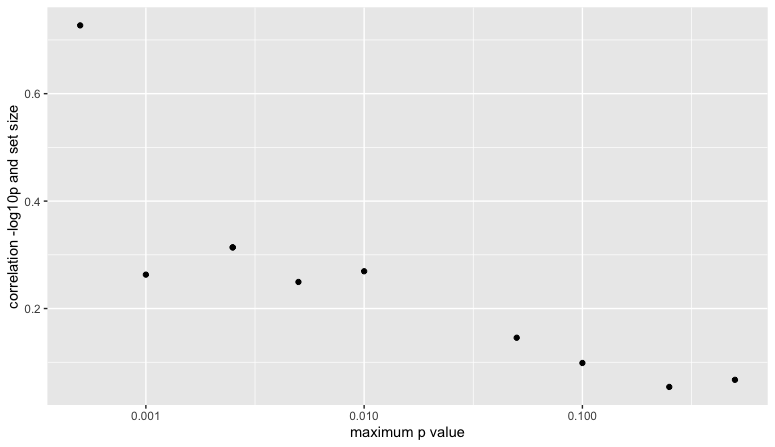
\includegraphics[width=12cm]{images/chapter2/ggplot/Rplot_corr_log10_set_p.png}
    \caption{Correlation of gene significance and set size with decreasing p. X axis maximum p value, y Pearsons correlation between -log10(p) of sets and set size. Data from supplementary material Sniekers et al\cite{sniekers2017genome}}
    \label{fig:correlation gene significance and set size Sniekers}
    \end{subfigure}
    
  \begin{subfigure}{15cm}
    \centering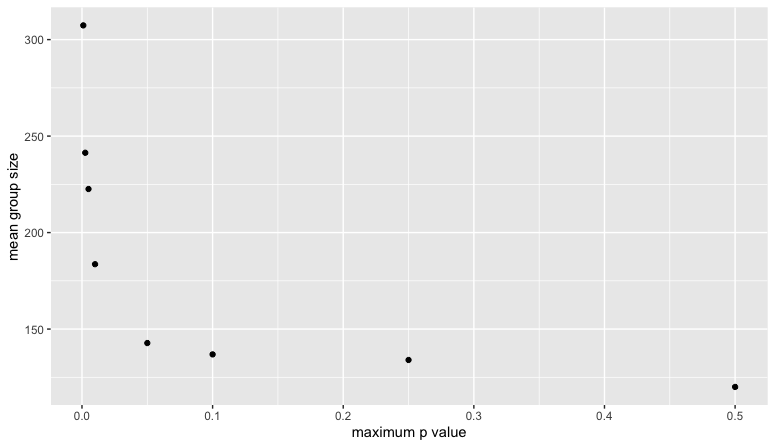
\includegraphics[width=12cm]{images/chapter2/ggplot/Rplot_minimum_p_mean_group_sizes.png}
    \caption{Changes in mean gene set size with decreasing maximum p values. Mean gene size increases. }
  \end{subfigure}
  \caption{Correlation between gene size and level of significance in MAGMA GSA and changes in mean gene size with increasingly significant gene sets (max p).Data from supplementary material Sniekers et al\cite{sniekers2017genome}}
   \label{fig:correlation gene significance and set size Sniekers with changes mean gene}
  \end{figure}


% \begin{figure}
%   \begin{subfigure}{8cm}
%     \centering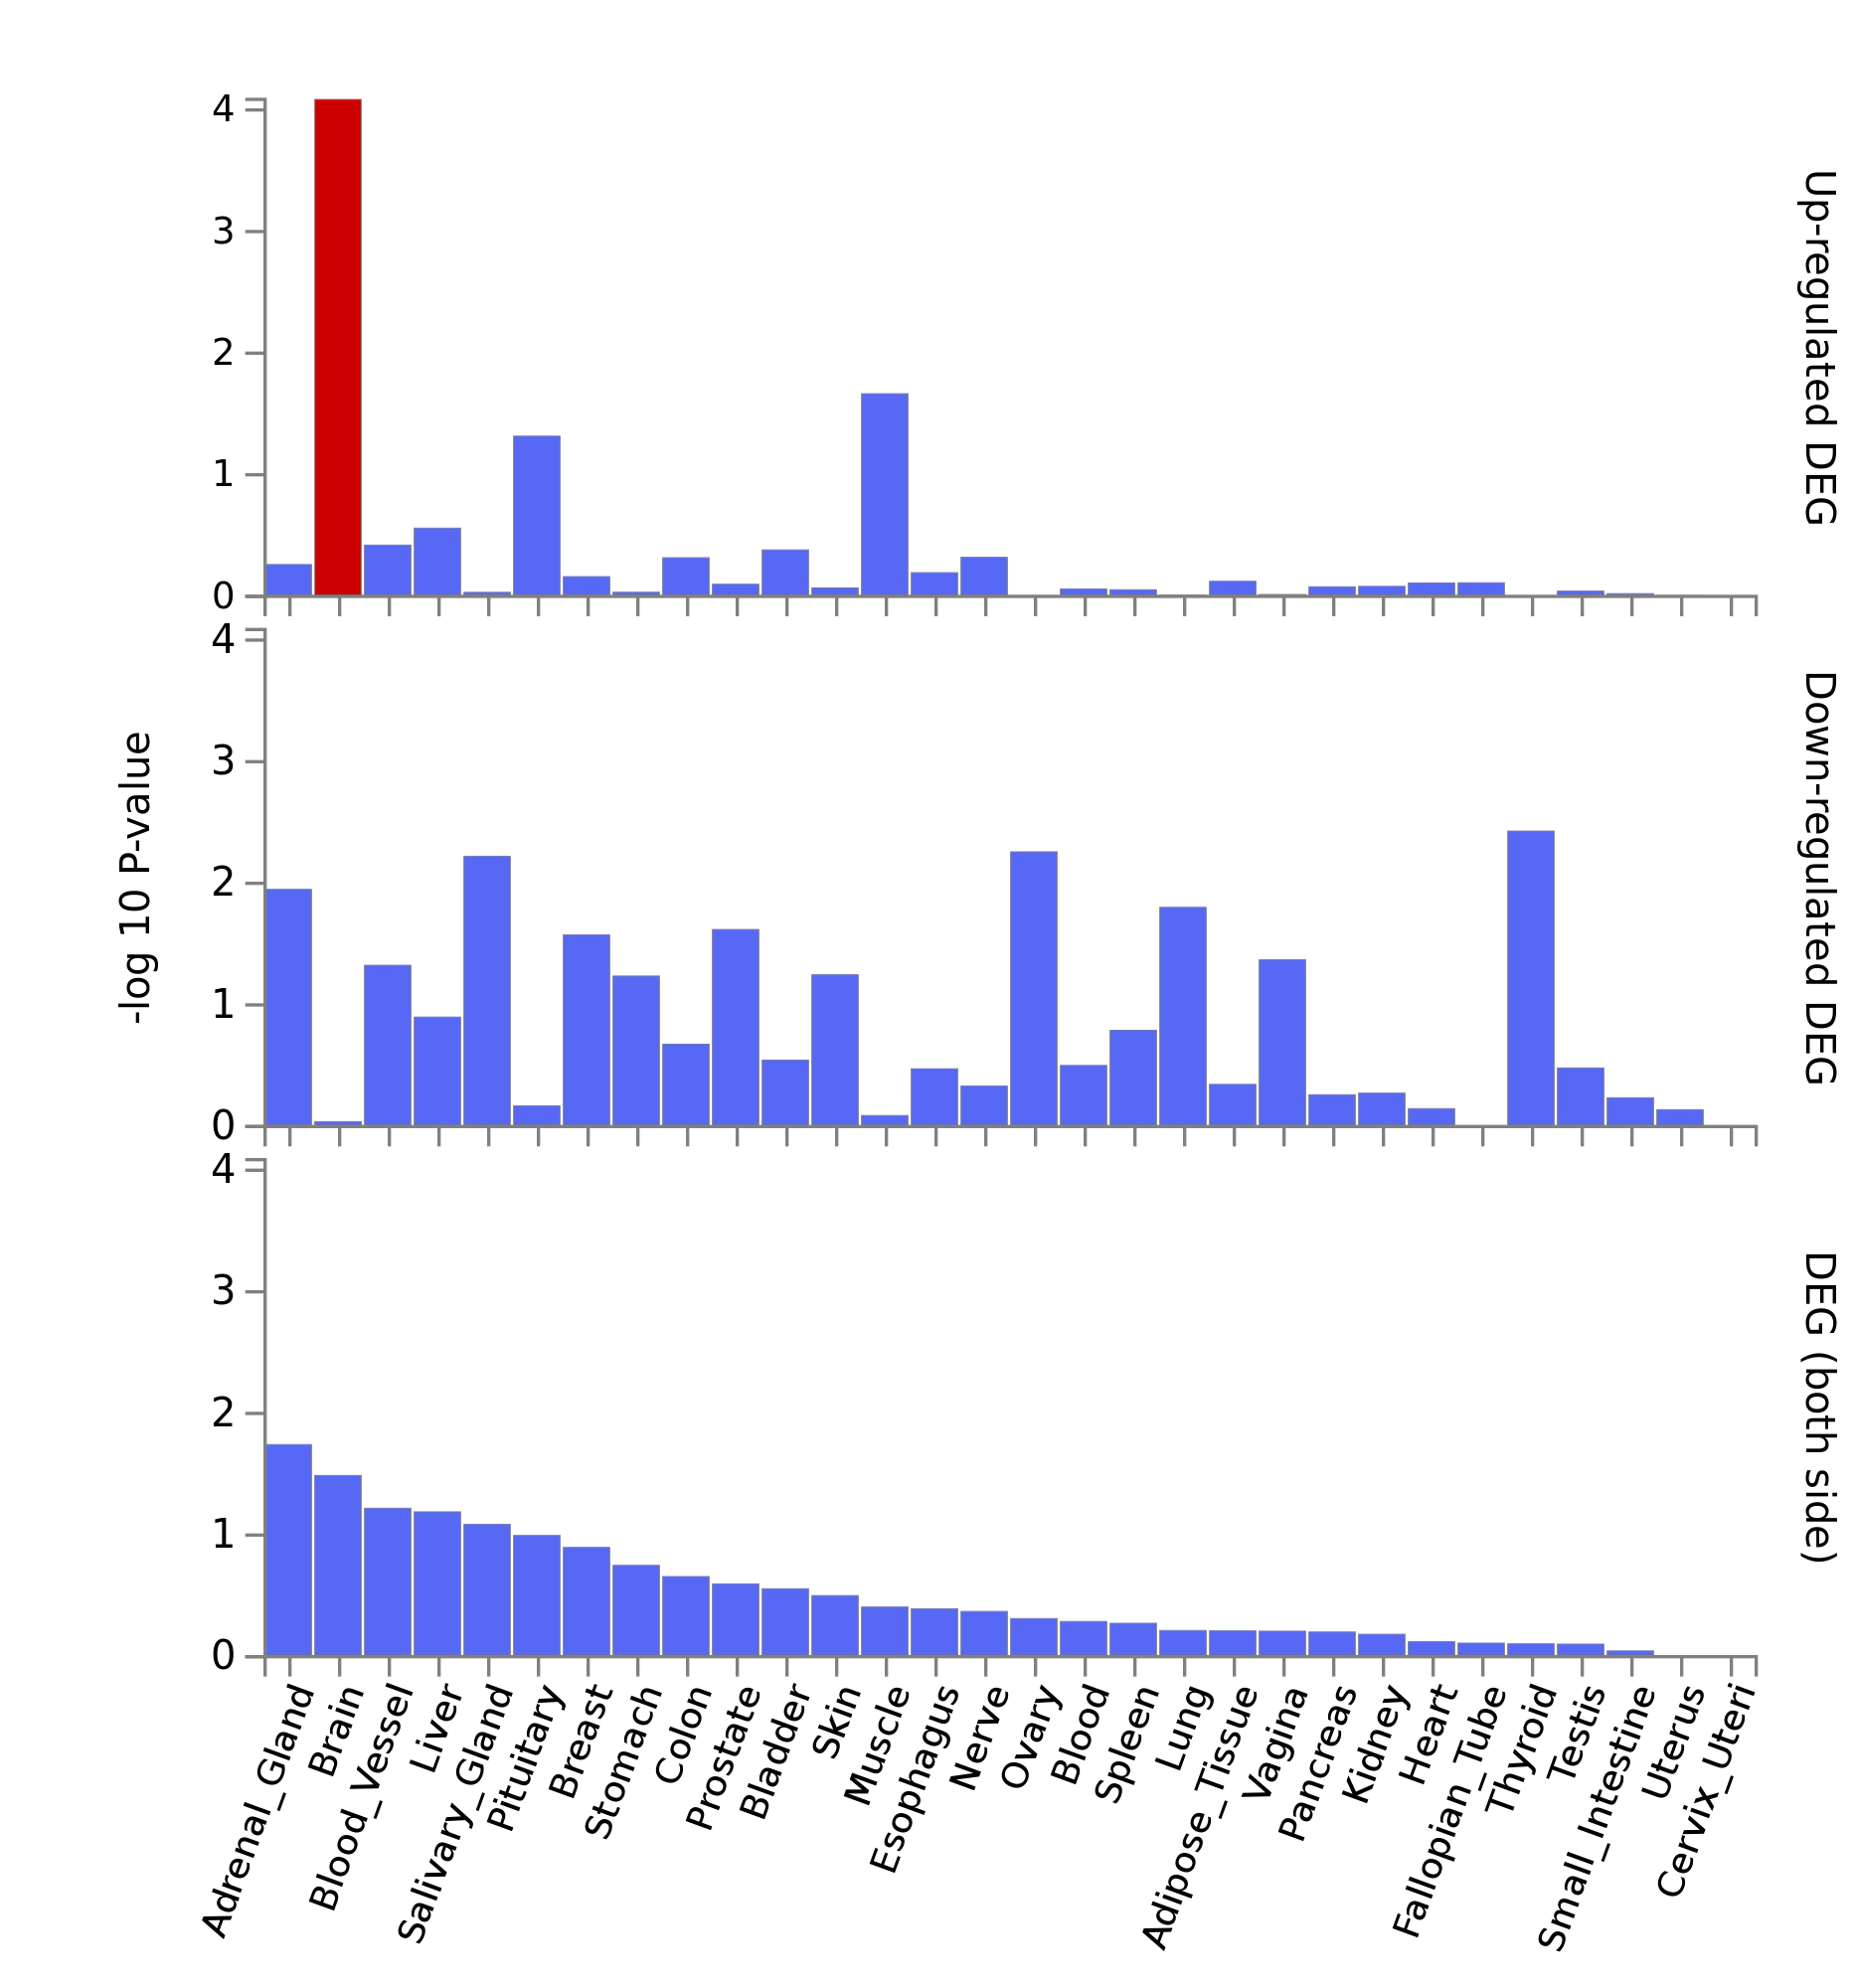
\includegraphics[width=7cm]{images/FUMA_plots/gtex_v8_ts_general_FUMA_gene2func_UKBBEd_syn_protein_bp_sig.png}
%     \caption{Gene expression UKBBEd significant genes}
%     \end{subfigure}
%   \begin{subfigure}{8cm}
%     \centering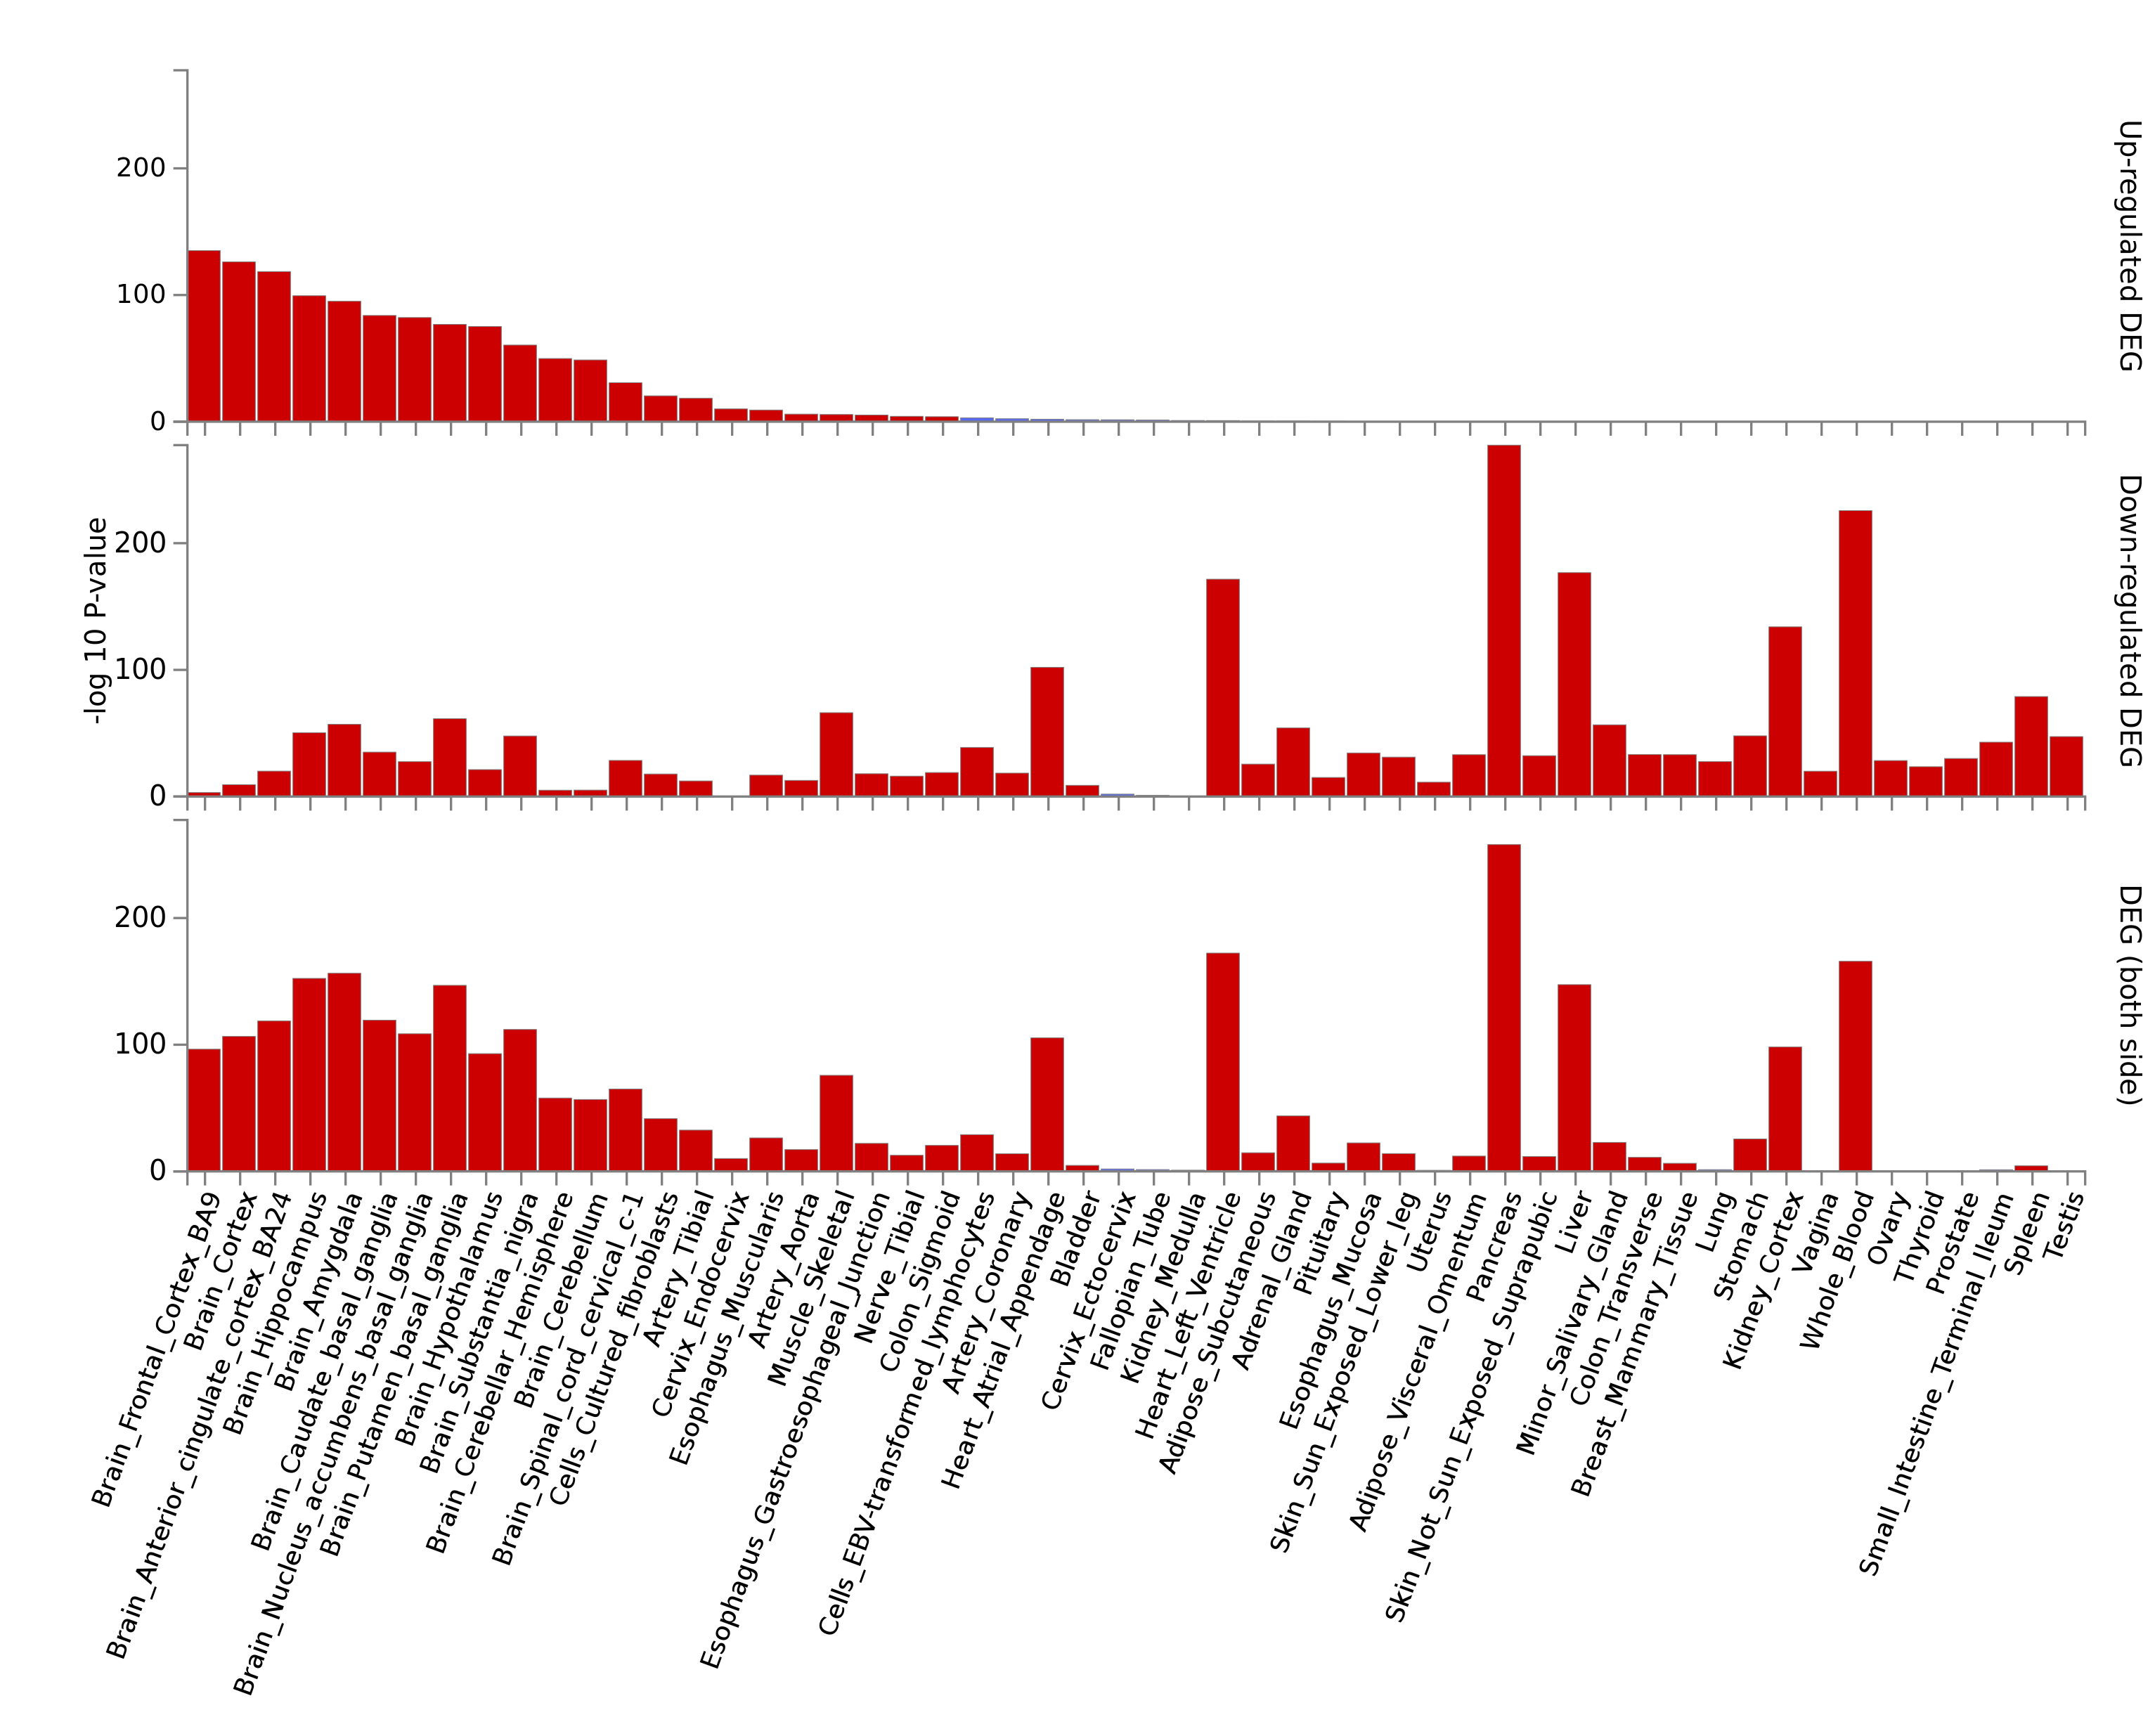
\includegraphics[width=7cm]{images/FUMA_plots/gtex_v8_ts_FUMA_PSP_gtex.png}
%     \caption{Genes in PSP}
%   \end{subfigure}
 
%   \begin{subfigure}{8cm}
%     \centering\includegraphics[width=7cm]{images/FUMA_plots/gtex_v8_ts_psp_not_consensus_FUMA_gene2func44650.png}
%     \caption{Genes in PSP but not in consensus PSD. ie new genes}
%   \end{subfigure}
%   \begin{subfigure}{8cm}
%     \centering\includegraphics[width=7cm]{images/FUMA_plots/gtex_v8_ts_1313_consensus_FUMA_gene2func44650.png}
%     \caption{Genes in consensus PSD}
%   \end{subfigure}
% \end{figure}
%  \todo[inline]{the bottom two expression profiles look too similar redo these}
 

 
 
 

  


\clearpage


\section{Discussion}
\label{sec:Methods Discussion}

 I will briefly discuss here the results that arise from this chapter (ostensibly a methods chapter). They are, however, integral to methods in the two following chapters. 

The results obtained using MAGMA GSA correspond closely to those reported in the  literature despite probable variations in versions, platforms and reference panels. In addition results from the PASCAL scoring algorithm correlate closely with those from MAGMA. 

Most elements identified in the PSP are found in the largest connected components and the disconnected genes excluded  are few in number and show no evidence of possessing common features that might make them sources of bias. Similarly only a few PSP genes do not have boundaries defined in the reference gene boundaries used for MAGMA and again they show no evidence of common features. 

The relative lack of statistically significant gene associations on MAGMA GSA suggest it would be reasonable to try to reduce unnecessary comparisons. One way of doing this is a discovery and replication cohort design and only testing synaptic topological sets we have a reason to believe would be enriched. 

6155 gene set results are found for MAGMA GSA in the supplemental material for Sniekers et al\cite{sniekers2017genome}. This is quite an exhaustive search over possible gene sets and the uncorrected p values provide a rough guide to likely significance levels in this sample (this is the only sample with published MAGMA GSA for the sample.) 365 gene sets are of greater than nominal significance (5.91\% of terms). Given there is no reason to expect a \textit{particular} network community defined only by topology to be associated with this particular phenotype (intelligence or educational attainment) and that there should be around 15 to 120 gene sets in a network (see chapter 4) then assuming this is a \textit{rough} guide to the distribution of significance levels using nominal significance to select sets as interesting and for further testing with correction for multiple comparisons would result in taking between 1-6 sets forward for testing which should limit type II error. 

Where does the figure of 15-120 gene sets come from? It is a rough estimation based on experience using community detection methods in a pilot study (not shown) and extrapolation from studies such as McLean et al. (2016) \cite{mclean2016improved}. Given that these are rough estimates another might be to look at the named synaptic groups used by Hill et al.\cite{hill2014human} other than the combined PSP.  Their average size is 65.75 genes. For the 3457 PSP this would result in 53.2 gene sets. In chapter~\ref{chap:community detection} I will address the expected number of gene sets in greater detail but these seem a reasonable rule of thumb. 

The lowest $p$ value found in any of the samples using the 18 member functionally defined synaptic set was 0.005 (Excitability Education\textsubscript{Discovery}) and occured in the best powered cohort. This group also did not have the constraint of forming a topological unit (it was not required to be a ``functional module'' (members forming a complete subgraph) never mind the stricter requirement of forming a community. (see section~\ref{sec:analysis of likely signal} and table~\ref{tab:table from hill})

It is noteworthy that few gene sets have been found to be significant in MAGMA GSA studies and those that are are very large (see table~\ref{tab:group size and enrichment} there is also an association between group size and significance (figure~\label{fig:correlation gene significance and set size Sniekers} and figure~\ref{fig:correlation gene significance and set size Sniekers with changes mean gene}) . The significance level of the NMDA receptors reported by Hill et al. \cite{hill2014human} was $p=0.002$. Assuming the PSP was divided into groups of similar size to the subgroups (ie not complete PSD) in the Hill paper the significance level using simply a Bonferroni correction for multiple comparisons would be  0.00094 for $n$=53 groups. 


\todo{Phrase better following footnote ? move or leave out}\footnote{On reflection this bit probably belongs in community detection or the discussion chapter and needs to be better phrased. - There is also a reductio argument in favour of a discovery and replication design.  A community detection might result in 100 groups of approximately size 35 or two groups one of 35 and the other of 3422. Let us assume that the size 35 group is relevant to the phenotype in ground truth. Let us then consider another clustering where all of the groups are around 35 in size and the one with the ground truth mapping to the phenotype we are interested in is there. There are also several other groups that map to diseases we are not testing, some to no disease but interesting functional groups and some novel but interesting groupings. 

Testing for the association with the phenotype using the evenly divided group with several interesting communities (although not all of interest to us)  would have a Bonferroni correction alpha level of 0.0005. The one dividing the network into one group of 35 and another of 3422 s would have an alpha level of 0.025. It is surely plausible that in testing a single phenotype the first group \textit{may} be the better clustering and its remaining 99 groups are enriched for other processes and disorders, the community detection method however that divides it into two groups would do far better even although its treatment of the non involved nodes does not best conform to their functional division. I return to this point in chapter~\ref{chap:community detection}.
\url{ source('~/RProjects/chapter2_checks/R/expected_gsa/ctg_size_plots.R')}}

SynGO shows the value of using less tests and more specific terms\footnote{adding syngo or a slim ontology on top of magma would be a pretty good msc project} (in particular for Education\textsubscript{Discovery} Biological Process in particular with much stronger enrichment than GO enrichment in ToppGene.\footnote{ Would be reasonable to try to add both a slim ontology and testing through the dag on top of magma or pascal. However although the FDR q value is lower there is not much specificity of the terms. }



Re-Analysis of the gene level scores of significant genes in GWGAS studies of intelligence and education suggest that around 25\% of these genes are in the post synaptic proteome. We would therefore expect that given the involvement of non PSP genes that the raw P values for enrichment would be less than those reported in Sniekers et al and other studies. I shall return to why this is important in further discussions (in brief intelligence and education get uniquely large sample sizes so can afford to trade power for conservatism, this will not be true of rarer diseases, if you get no significant GSA in a study with 78000 people the technique will be of little use for diseases other than the very commonets). 

The gene sets with very low unadjusted p values in these studies tend also to be much larger than those we would find in the PSP and there is a correlation between gene size and log10p.

Disease terms related to intellectual disability are found in both education samples and neither intelligence sample. An association is reported in Sniekers et al. \cite{sniekers2017genome} using DEPICT but I am not aware that the difference with intelligence samples has been reported. It does suggest there may be a qualitative difference between enriched genes in the education and intelligence samples in addition to the difference in genetic correlation of the two phenotypes.  

PSP genes are expressed robustly in all brain regions using the GTEx data and this suggests that the increase in gene number in the network has still resulted in a set of genes strongly expressed in the CNS. The pattern of correlation of gene expression between brain regions in the PSP is similar to that recorded of all genes literature \cite{mele2015human} suggesting that we do not have a very unusual sample.  

\footnote{This to discussion of chapter community detection or intro Finally the lack of over representation o
lack of over representation of synaptic elements on GSA of significant genes despite evidence of synaptifc involvement using polygenic signal shows limitations of even using GWAS catalog for network studies}

\todo[inline]{cross ref for this section}



\todo{in discussion mention that although synapse and PSP only 25\% it is the only system enriched}




\clearpage
\todo[inline]{text to be moved commented out to print}
% this is discussion discussion move \todo{this is the bit on tissue specificity may move to end of thesis discussion}
% Disease associated genes are more likely to be uniquely expressed in a tissue according to several references cited by Kitsak et al.\footnote{note to self this is kitsak and ghissian and menche and barabasi - they use a mixture of PPI and other networks (from menche) they use their own definition of tissue expressed which is one tissue with z>1 where z is z score. See comment on gtex} \todo{move some of this to discussion} Finally, the most similar analysis to ours \cite{ghiassian2015disease} whose first author is one of the coauthors in the paper by Kitsak et al.\cite{kitsak2016tissue} uses a network of heterogenous interactions. One of the potential limitations of the authors' approach was using a network composed of a combination of experimental protein interactions, predicted reactions and other networks such as metabolic networks found in KEGG (a non tissue specific proteome network used across a variety of diseases). 
% also see \cite{luck2020reference}
% \cite{tran2019condition}
\clearpage
\section{To supplemental tables}
\begin{table}[ht]
\centering
\begin{tabular}{lrrr}
  \toprule
Gene set name & n genes & $\beta$ & p \\ 
  \midrule
Exocytosis & 83 & 0.19 & 0.039 \\ 
  Neurotransmitter metabolism & 27 & -0.10 & 0.686 \\ 
  Excitability & 57 & 0.38 & 0.005 \\ 
  Protein cluster & 43 & 0.20 & 0.091 \\ 
  Ligand-gated ion channel signaling & 33 & 0.03 & 0.438 \\ 
  Tyrosine kinase signaling & 7 & 0.22 & 0.308 \\ 
  Unassigned & 59 & 0.07 & 0.301 \\ 
  Peptide/neurotrophin signals & 28 & 0.04 & 0.430 \\ 
  Intracellular signal transduction & 148 & -0.04 & 0.697 \\ 
  Ion balance/transport & 41 & -0.01 & 0.522 \\ 
  G-protein relay & 27 & -0.10 & 0.688 \\ 
  RNA and protein synthesis, folding and breakdown & 67 & 0.01 & 0.448 \\ 
  Endocytosis & 25 & -0.17 & 0.804 \\ 
  Structural plasticity & 95 & -0.06 & 0.731 \\ 
  Cell metabolism & 51 & -0.13 & 0.827 \\ 
  Cell adhesion and trans-synaptic signaling & 76 & 0.29 & 0.009 \\ 
  G-protein-coupled receptor signaling & 41 & 0.09 & 0.300 \\ 
  Intracellular trafficking & 75 & 0.04 & 0.344 \\ 
   \bottomrule
\end{tabular}
\caption{Synaptic enrichment UKBB int Source\url{source('~/RProjects/redo_chapter2/R/redo_synapse_set_int_curated.R')}} 
\label{tab:MAGMA enrichment of synaptic groups UKBBint}
\end{table}

% latex table generated in R 3.6.3 by xtable 1.8-4 package
% Sun Aug  9 12:41:54 2020
\begin{table}[ht]
\centering
\begin{tabular}{lrrr}
   \toprule
Gene set name & n genes & $\beta$ & p\\
  \midrule
Exocytosis & 83 & 0.04 & 0.348 \\ 
  Neurotransmitter metabolism & 27 & -0.08 & 0.648 \\ 
  Excitability & 57 & 0.43 & 0.003 \\ 
  Protein cluster & 43 & -0.14 & 0.813 \\ 
  Ligand-gated ion channel signaling & 33 & 0.18 & 0.178 \\ 
  Tyrosine kinase signaling & 7 & -0.18 & 0.658 \\ 
  Unassigned & 59 & 0.08 & 0.276 \\ 
  Peptide/neurotrophin signals & 28 & -0.20 & 0.828 \\ 
  Intracellular signal transduction & 148 & 0.07 & 0.226 \\ 
  Ion balance/transport & 41 & 0.11 & 0.242 \\ 
  G-protein relay & 27 & -0.09 & 0.671 \\ 
  RNA and protein synthesis, folding and breakdown & 67 & 0.10 & 0.198 \\ 
  Endocytosis & 25 & 0.12 & 0.281 \\ 
  Structural plasticity & 95 & 0.04 & 0.355 \\ 
  Cell metabolism & 51 & 0.05 & 0.374 \\ 
  Cell adhesion and trans-synaptic signaling & 76 & 0.39 & 0.001 \\ 
  G-protein-coupled receptor signaling & 41 & -0.01 & 0.517 \\ 
  Intracellular trafficking & 75 & -0.06 & 0.713 \\ 
   \hline
   \bottomrule
\end{tabular}
\caption{Synaptic enrichment UKBB Ed} 
\label{tab:MAGMA enrichment of synaptic groups UKBBEd}
\end{table}0.016 

% latex table generated in R 3.6.3 by xtable 1.8-4 package
% Sun Aug  9 12:43:33 2020
\begin{table}[ht]
\centering
\begin{tabular}{lrrr}
  \toprule 
Gene set name & n genes & $\beta$ & p\\
  \midrule
Cell adhesion and trans-synaptic signaling & 76 & 0.11 & 0.155 \\ 
  Cell metabolism & 51 & -0.07 & 0.726 \\ 
  Endocytosis & 25 & -0.03 & 0.572 \\ 
  Excitability & 57 & 0.13 & 0.159 \\ 
  Exocytosis & 83 & 0.18 & 0.016 \\ 
  G-protein-coupled receptor signaling & 41 & 0.15 & 0.162 \\ 
  G-protein relay & 27 & 0.11 & 0.251 \\ 
  Intracellular signal transduction & 148 & 0.07 & 0.150 \\ 
  Intracellular trafficking & 75 & -0.01 & 0.522 \\ 
  Ion balance/transport & 41 & -0.17 & 0.898 \\ 
  Ligand-gated ion channel signaling & 33 & -0.27 & 0.944 \\ 
  Neurotransmitter metabolism & 27 & 0.25 & 0.099 \\ 
  Peptide/neurotrophin signals & 28 & -0.10 & 0.720 \\ 
  Protein cluster & 43 & 0.11 & 0.207 \\ 
  RNA and protein synthesis, folding and breakdown & 67 & 0.11 & 0.120 \\ 
  Structural plasticity & 95 & -0.10 & 0.874 \\ 
  Tyrosine kinase signaling & 7 & -0.45 & 0.880 \\ 
  Unassigned & 58 & -0.03 & 0.620 \\ 
   \bottomrule
\end{tabular}
\caption{Synaptic enrichment ctg} 
\label{tab:MAGMA enrichment of synaptic groups ctg}
\end{table}

% latex table generated in R 3.6.3 by xtable 1.8-4 package
% Sun Aug  9 12:45:12 2020
\begin{table}[ht]
\centering
\begin{tabular}{lrrr}
  \toprule
Gene set name & n genes & $\beta$ & p\\
  \midrule
Cell adhesion and trans-synaptic signaling & 76 & 0.17 & 0.067 \\ 
  Cell metabolism & 53 & -0.02 & 0.549 \\ 
  Endocytosis & 26 & 0.11 & 0.251 \\ 
  Excitability & 57 & 0.16 & 0.122 \\ 
  Exocytosis & 83 & -0.11 & 0.877 \\ 
  G-protein-coupled receptor signaling & 41 & 0.08 & 0.315 \\ 
  G-protein relay & 27 & -0.01 & 0.521 \\ 
   Intracellular signal transduction & 147 & 0.02 & 0.418 \\ 
  Intracellular trafficking & 75 & -0.02 & 0.590 \\ 
  Ion balance/transport & 40 & 0.05 & 0.370 \\ 
  Ligand-gated ion channel signaling & 33 & 0.18 & 0.158 \\ 
  Neurotransmitter metabolism & 27 & -0.15 & 0.774 \\ 
  Peptide/neurotrophin signals & 28 & 0.11 & 0.267 \\ 
  Protein cluster & 42 & -0.20 & 0.910 \\ 
  RNA and protein synthesis, folding and breakdown & 66 & 0.22 & 0.016 \\ 
  Structural plasticity & 95 & 0.10 & 0.140 \\ 
  Tyrosine kinase signaling & 7 & -0.27 & 0.742 \\ 
  Unassigned & 58 & 0.07 & 0.290 \\ 
   \bottomrule
\end{tabular}
\caption{Synaptic enrichment EA2} 
\label{tab:MAGMA enrichment of synaptic groups EA2}
\end{table}
\clearpage
\begin{figure}
    \centering
    \includegraphics[height=25cm]{images/FUMA_plots/expHeat_FUMA_gene2func-2_ukbbed_zeromean.png}
    \caption{Heatmap gene expression FUMA UKBBEd Average value of the relavitve expression level zero mean centred and log2 transformed. Shows that a small number of genes amongst those enriched are very enriched}
    \label{fig:my_label}
\end{figure}
% \begin{table}[]
%     \centering
%     \begin{tabular}{llll}
%     \toprule
%     Number & First author & Year & Citation\\
%     \midrule
%       1  &  PENG & 2002 & \cite{peng2004semiquantitative}  is 2004 \\
%       2  &  SATON  2002    is SATOH &2002 &\cite{satoh2002identification} \\
%     3 &  SCHWENK & 2013 &  \cite{schwenk2012high} 2012\\
%     4 &  SELIMI  & 2009 & \cite{selimi2009proteomic} \\
%     5 &  TRINIDAD & 2005& \cite{trinidad2005phosphorylation} \\  
% 6& TRINIDAD  &2008 & \cite{trinidad2008quantitative} \\
% 7&  WALIKONIS & 2000&  \cite{walikonis2000identification}\\ 
%  8 &YOSHIMURA &2004& \cite{yoshimura2004molecular}   \\
% 9 &FROMER &2014 & \footnote{Not in Heil I only find fromer in an oksana paper on PSD and it is on scz I assume this is Focking and the one cited in Heil is bipolar
% and they have 2033} PSD proteins Focking \cite{focking2016proteomic}\\
% 10&FARR &2004 &  \cite{farr2004proteomic}\\
% 11&Distler.PSDII & 2014 &\cite{distler2014depth}\\
% 12& BAYES & 2011&    \cite{bayes2011characterization}  \\
% 13 &  BAYES &2012 & \cite{bayes2012comparative}  \\  
% 14& COLLINS &2006 & \cite{collins2006molecular}\\
% 15 & DOSEMECI  &2007&  \cite{dosemeci2007composition}\\
% 16 & FERNANDES  &2009&  \cite{fernandez2009targeted}\\
% 17 & BAYES &2014 &  \cite{bayes2014human}\\
% \bottomrule
%     \end{tabular}
%     \caption[Primary proteomic studies contributing to the PSP graph]{Primary proteomic studies contributing to the PSP graph \footnote{to Douglas: if using the Oksana Clean Published data TO REMOVE please see note on text}}
%     \label{tab:oksana clean published}
% \end{table}


\begin{table}[]
    \centering
    \begin{tabular}{llllllll}
    \toprule
     & First author & Year & Reference & Region & Species & $n$ & In Oksana file \\
    \midrule
1 &    WALIKONIS &2000 &Walikonis et al. (2000)\cite{walikonis2000identification} &postsynapse & rat & 29 \\
2 &PENG&2004&Peng et al. (2004) \cite{peng2004semiquantitative}&postsynapse& rat& 325\\
3 &SATOH&2002&Satoh et al. (2002)\cite{satoh2002identification} &postsynapse &mouse &45\\
4 &YOSHIMURA&2004&Yoshimura et al. (2004) \cite{yoshimura2004molecular} &postsynapse& rat &435\\
5 &FARR&2004&Farr et al. (2004)  \cite{farr2004proteomic}&postsynapse &rat &71 &Yes\\
6 &JORDAN&2004&Jordan et al. (2004)&postsynapse &mouse and rat &390& NOT\\
7&LI&2004 &wan Li et al. (2003)&postsynapse &rat& 137& NOT\\
8&TRINIDAD&2005 &Trinidad et al. (2005) \cite{trinidad2005phosphorylation}&postsynapse&mouse& 234& YES\\
9&CHENG&2006&Cheng et al. (2006)&postsynapse& rat& 288& NO\\
10&COLLINS&2006&Collins et al. (2006)\cite{collins2006molecular}&postsynapse &mouse& 717& YES\\
11&DOSEMESI&2006&Dosemeci et al. (2006)&postsynapse& rat& 113& NO\\
12&DOSEMESI&2007&Dosemeci et al. (2007)&postsynapse& rat& 548& YES\\
13&TRINIDAD&2008&Trinidad et al. (2008)&postsynapse& mouse& 2150& YES\\
14&SELIMI&2009&Selimi et al. (2009)\cite{selimi2009proteomic}&postsynapse &mouse &61& YES\\
15&FERNANDEZ&2009&Fernández et al. (2009)  \cite{fernandez2009targeted}&postsynapse& mouse &292& YES\\
16&BAYES&2010&Bayés et al. (2011)&postsynapse &human &1441& YES\\
17&BAYES&2012&Bayés et al. (2012)&postsynapse &mouse &1545 &YES\\
18&SCHWENK&2012&Schwenk et al. (2012) \cite{schwenk2012high}&postsynapse &unknown &34& YES\\
19&DISTLER PSD1*&2014&Distler et al. (2014)&postsynapse& mouse& 3545& NO \footnote{intended per email}\\
20&DISTLER PSD2*&2014&Distler et al. (2014)&postsynapse& mouse& 2092*& Oksana\\
21&BAYES&2014&Bayés et al. (2014)&postsynapse& human &1141& YES\\
22&UEZU&2016&Uezu et al. (2016)&postsynapse &mouse &1111 &NO\\
23&FOCKING&2016&Föcking et al. (2016)&postsynapse& human &2026 &NO\\
\bottomrule
    \end{tabular}
    \caption[Primary Proteomic studies appearing in PSP cleaned from Heil (2018)]{Primary proteomic studies contributing to the PSP take from Heil 2018\cite{heil2018systems} from Katharina PhD p84 table 5.1. \footnote{to Douglas: These should have been the same as given to me as per email from Colin need to chose one see note on text. Distler PSD1 is definitely dropped from the cleaned data. The graph is somewhere between these two points. The most conservative is the Oksana one.}}
    \label{tab:Katharina_phd_studiesFF}
\end{table}
% \section{NOT IN DOCUMENT}
% \section{FRAMEWORK FOR GSA - USED}
% %%% FRAMEWORK
% \section{Gene Ontology Analysis of MAGMA genes FRAMEWORK}
% They are not all measured the same way eg DEPICT in Okbay so worth going through 

% Is the gtex higher in both education
%     \subsection{Intelligence Replication}
%         \subsubsection{Authors findings}
%         MAGMA Regulating cell development $P=3.5 \times 10^{-6}$. Authors state that several (?14) of the significant genes are more expressed in the CNS.
%         \subsubsection{Ontology ORA Genome}
%         \paragraph{Toppgene ToppFun Intelligence Replication}
%         \subparagraph{ToppFun BP} nil
%         \subparagraph{ToppFun MF} nil
%         \subparagraph{ToppFun CC} See table~\ref{tab:cellular component in toppgene}
%         \begin{table}[ht]
%     \centering
%     \begin{tabular}{llllllll}
%          ID &Name 	&	pValue 	&FDR BH &	FDR BY 	&Bonferroni  	&n input & n annot  \\
%          GO:0032584 &	growth cone membrane\footnote{part of growth cone: distal axon: neuron projection:cell projection: cellular anatomical entity} &		1.416E-4 &	3.838E-2 &2.373E-1&	3.838E-2 &	2 &	8 \\
%     \end{tabular}
%     \caption{Cellular component in toppgene}
%     \label{tab:cellular component in toppgene}
% \end{table}
%         \paragraph{Panther Intelligence Replication}
%         All genes 47 identified
        
%         \subparagraph{Panther BP} nil
%         \subparagraph{Panther MF} nil
%         \subparagraph{Panther CC} Two terms Cytoplasm GO:0005737 n in annotation 11714 n in set	40; expected 	26.40 ; fold change	1.51 ;	+ 	; raw P4.29E-05 	; FDR 0.431 4.31E-02 and its parent term intracellular GO:0005622 n in annotation 14693 ; n in set	45 ; E	33.12 ; fold	1.36 ;	+ ;	3.24E-05 ; FDR	6.50E-02 Not significant


%         \subsubsection{Ontology ORA Synaptic}
        
%         \subsubsection{Others}
%         \begin{itemize}
%             \item path to code
%             \item GTex
%             \item Other phenotypes
%         \end{itemize}
        

%     \subsection{Education Replication}
%         \subsubsection{Authors findings Education Replication}
%         Pathways involving CNS development
%         13 Gtex tissues in CNS showed elevated expression of genes near EduYears SNPs
%         283 Gene sets. 5 clusters ``neural progenitor cells, migration of new neurons to cortex, projection of axons to target, sprouting of dendrites and spines and neuronal signalling and synaptic plastigcity throughout the lifespan'' not precis quote but close last group is the one of interest to use 
%         Genes prioritised by DEPICT. Overlap with ID and ASD.GRIK2<10e-6, CALM2 < 10e-4 PPI in Figure 3 ?includes multiple testing. 685 genes at 273 Loci p 88 of supplemental material supplementary table 4.1 wherever that is. We have not used this approach as \url{https://github.com/perslab/gwas-snps-loci} as predominant approach is MAGMA.
%         \subsubsection{Ontology ORA Education Replication Genome}
%       \paragraph{toppgene}
%           \subparagraph{BP toppgene}  See table~\ref{tab:BP EA2 all significant toppgene} 
%             \begin{table}[ht]
% \centering
% \begin{tabular}{rllrrrr}
%   \hline
%  & ID & Name & test & Genome & p & Bon \\ 
%   \hline
% 1 & GO:0022008 & neurogenesis & 26 & 1866 & $5.97 \times 10^{-7}$ & 0.00176 \\ 
%   2 & GO:0042063 & gliogenesis & 11 & 352 & $1.14 \times 10^{-6}$ & 0.00337 \\ 
%   3 & GO:0007417 & central nervous syst & 19 & 1129 & $1.81 \times 10^{-6}$ & 0.00535 \\ 
%   4 & GO:0048666 & neuron development & 20 & 1297 & $3.53 \times 10^{-6}$ & 0.01041 \\ 
%   5 & GO:0010001 & glial cell different & 9 & 261 & $5.16 \times 10^{-6}$ & 0.01522 \\ 
%   6 & GO:0050808 & synapse organization & 12 & 498 & $5.39 \times 10^{-6}$ & 0.01589 \\ 
%   7 & GO:0048667 & cell morphogenesis i & 14 & 688 & $5.92 \times 10^{-6}$ & 0.01747 \\ 
%   8 & GO:0048699 & generation of neuron & 23 & 1751 & $8.43 \times 10^{-6}$ & 0.02489 \\ 
%   9 & GO:0048812 & neuron projection mo & 14 & 742 & $1.39 \times 10^{-5}$ & 0.04100 \\ 
%   10 & GO:0010771 & negative regulation  & 6 & 109 & $1.53 \times 10^{-5}$ & 0.04527 \\ 
%   \hline
% \end{tabular}
% \caption{BP EA2 all significant Toppgene 99 genes in total \url{source('~/RProjects/paper_xls_output/R/chapter_2/eda_toppgene_all_significant_ea2.R')}} 
% \label{tab:BP EA2 all significant toppgene}
% \end{table}

% \subparagraph{CC toppgene}
% See table~\ref{tab:CC EA2 all significant Toppgene}
% % latex table generated in R 3.6.3 by xtable 1.8-4 package
% % Wed Aug 19 12:29:17 2020
% \begin{table}[ht]
% \centering
% \begin{tabular}{llrrrr}
%   \hline
% ID & Name & test & Genome & p & Bon \\ 
%   \hline
% GO:0098794 & postsynapse & 16 & 825 & $1.46 \times 10^{-6}$ & 0.00050 \\ 
%   GO:0045202 & synapse & 20 & 1482 & $1.58 \times 10^{-5}$ & 0.00547 \\ 
%   \hline
% \end{tabular}
% \caption{CC EA2 all significant Toppgene \url{source('~/RProjects/paper_xls_output/R/chapter_2/eda_toppgene_all_significant_ea2.R')} }
% \label{tab:CC EA2 all significant Toppgene}
% \end{table}


        
%     \paragraph{panther}
%     Panther by default uses HGNC numerical symbols so it is necessary to prefix Entrez ID with GeneID: this is done in a custom R script \url{source('~/RProjects/paper_xls_output/R/chapter_2/exploratory_data_analysis.R')}
%     Unmapped Gene ID using entrez with Gene ID prefix
%     GeneID:246744

%         \subparagraph{BP Panther}
%         BP panther ordered by FDR 19 items top Nervous system development FDR 0.006 (2430 genes in reference) 2.57 fold change (see table~\ref{tab:GO.biological.process.complete Panther Gene Ontology Enrichment significant genes in Education Replication}). The heirarchy of terms in gene ontology is shown in figure~\ref{fig:panther GO Biological Process Heirarchy shown}\footnote{Douglas: I have included this as a screenshot. Parsing the xml and getting it into latex took longer than I thought so I went straight to screenshot as a last resort could do the indentation by hand. Thought worth showing (as DEPICT, MAGMA etc as far as I can see ignore heirarchy) but interested in what you thought. The standard table output for panther doesn't have the heirarchy.}
        
%         \begin{figure}
%             \centering
%             \includegraphics[width=\textwidth]{images/screenshots/EA2_BP_Panther_all_genes.png}
%             \caption{Panther GO Biological Process EA2 Hierarchy shown. This includes all genes accessed by manually editing the Gene Symbol}
%             \label{fig:panther GO Biological Process Heirarchy shown}
%         \end{figure}
%         % latex table generated in R 3.6.3 by xtable 1.8-4 package
% % Sun Aug 23 11:12:46 2020
% \begin{table}[ht]
% \centering
% \begin{tabular}{lrrrlrcc}
%   \hline
% GO.biological.process.complete & ref & test & [E] & ou & fold & P & FDR \\ 
%   \hline
% nervous system development (GO:0007399) & 2430 & 30 & 11.7 & + & 2.57 & $7.62 \times 10^{-7}$ & 0.006 \\ 
%   neuron development (GO:0048666) & 848 & 17 & 4.1 & + & 4.18 & $6.68 \times 10^{-7}$ & 0.011 \\ 
%   neuron differentiation (GO:0030182) & 1046 & 18 & 5.0 & + & 3.59 & $2.58 \times 10^{-6}$ & 0.014 \\ 
%   negative chemotaxis (GO:0050919) & 46 & 5 & 0.2 & + & 22.66 & $4.42 \times 10^{-6}$ & 0.014 \\ 
%   neurogenesis (GO:0022008) & 1690 & 23 & 8.1 & + & 2.84 & $4.42 \times 10^{-6}$ & 0.018 \\ 
%   \makecell{negative regulation of cell morphogenesis\\ involved in differentiation (GO:0010771)} & 100 & 6 & 0.5 & + & 12.51 & $1.18 \times 10^{-5}$ & 0.031 \\ 
%   generation of neurons (GO:0048699) & 1585 & 21 & 7.6 & + & 2.76 & $1.88 \times 10^{-5}$ & 0.037 \\ 
%   regulation of synapse structure or activity (GO:0050803) & 240 & 8 & 1.1 & + & 6.95 & $2.51 \times 10^{-5}$ & 0.040 \\ 
%   regulation of synapse organization (GO:0050807) & 229 & 8 & 1.1 & + & 7.28 & $1.81 \times 10^{-5}$ & 0.041 \\ 
%   cell development (GO:0048468) & 1654 & 21 & 7.9 & + & 2.65 & $3.51 \times 10^{-5}$ & 0.043 \\ 
%   regulation of extent of cell growth (GO:0061387) & 115 & 6 & 0.6 & + & 10.88 & $2.51 \times 10^{-5}$ & 0.044 \\ 
%   regulation of axonogenesis (GO:0050770) & 192 & 7 & 0.9 & + & 7.60 & $4.77 \times 10^{-5}$ & 0.045 \\ 
%   negative regulation of axonogenesis (GO:0050771) & 72 & 5 & 0.3 & + & 14.48 & $3.37 \times 10^{-5}$ & 0.045 \\ 
%   regulation of cell size (GO:0008361) & 187 & 7 & 0.9 & + & 7.81 & $4.05 \times 10^{-5}$ & 0.046 \\ 
%   membrane protein proteolysis (GO:0033619) & 39 & 4 & 0.2 & + & 21.39 & $5.23 \times 10^{-5}$ & 0.046 \\ 
%   regulation of neuron projection development (GO:0010975) & 521 & 11 & 2.5 & + & 4.40 & $4.70 \times 10^{-5}$ & 0.047 \\ 
%   neuron projection development (GO:0031175) & 697 & 13 & 3.3 & + & 3.89 & $3.29 \times 10^{-5}$ & 0.048 \\ 
%   positive regulation of collateral sprouting (GO:0048672) & 12 & 3 & 0.1 & + & 52.13 & $4.60 \times 10^{-5}$ & 0.049 \\ 
%   regulation of neurogenesis (GO:0050767) & 847 & 14 & 4.1 & + & 3.45 & $5.84 \times 10^{-5}$ & 0.049 \\ 
%   \hline
% \end{tabular}
% \caption{GO.biological.process.complete Panther Gene Ontology Enrichment significant genes in Education Replication} 
% \label{tab:GO.biological.process.complete Panther Gene Ontology Enrichment significant genes in Education Replication}
% \end{table}
%             \subparagraph{MF panther} No significant
%             \subparagraph{CC panther} Only one term synapse GO:0045202 1382 terms in reference 19 in table expected 6.50 fold enrichment 29.93 raw P $2.29\times 10^{-5}$ FDR 0.0459

%         Compare with toppgene widely variant scores noted in \cite{rhee2008use} and detailed discussion in \cite{khatri2005ontological}
%          \subsubsection{Ontology ORA Synaptic}
%          \subsubsection{Others}
%          \paragraph{disease enrichment}
%          Enrichment in DisGeNNet BeFree searched by toppfun of Intellectual disability
%         ID C3714756 	Intellectual Disability ; Source	DisGeNET BeFree ; p 	8.884E-7 ; FDR BH	1.648E-3; FR BY 	1.386E-2 ;Bonferroni	2.237E-3; Input 	20 	Total 1219
        
%         % latex table generated in R 3.6.3 by xtable 1.8-4 package
% % Sun Aug 23 12:35:02 2020
% \begin{table}[ht]
% \centering
% \begin{tabular}{rllr}
%   \hline
% Entrez.Gene.ID & Gene.Symbol & Gene.Name & Original.Symbol \\ 
%   \hline
% 5144 & PDE4D & phosphodiesterase 4D & 5144 \\ 
%   5662 & PSD & pleckstrin and Sec7 domain containing & 5662 \\ 
%   4137 & MAPT & microtubule associated protein tau & 4137 \\ 
%   4208 & MEF2C & myocyte enhancer factor 2C & 4208 \\ 
%   4744 & NEFH & neurofilament heavy & 4744 \\ 
%   257194 & NEGR1 & neuronal growth regulator 1 & 257194 \\ 
%   \hline
% \end{tabular}
% \caption{Intellectual disability genes significant in EA2 found in PSP} 
% \label{tab:Intellectual disability genes significant in EA2 found in PSP}
% \end{table}
%         Path to code
        
%         GTEx
% \clearpage














% \subsection{Put problems with GSA multiple testing somewhere}
% \footnote{gsea moved to chapter 4}
% \subsection{PASCAL software}
% Need to check version on strontium. Original version. Alpha 0.1. 
% shell command
% default options 
% no gene boundary
% empirical method

% \todo[inline]{I think this goes to community detection}
% \section{Other models of topology}
% We may want to put the diamond bit in here on the basis that if that hypothesis is correct then diamond should be good but it isn't so on to what we are doing (and we can mention the similarity in the rejected bit) see section~\ref{sec:DIAMOnD algo} \todo[inline]{I think this goes to community detection}
%  \subsection{Analysis of likely signal}
% \label{sec:analysis of likely signal}
% The paper by Hill et al. \cite{hill2014human} testing synaptic components for enrichment for genetic variants associated with differences in intelligence adopts a discovery and replication cohort design. It is particularly noteworthy as it is a hypothesis driven use of GSA (GSEA here) to investigate the role of synaptic components in differences in human cognitive ability. It is further noteworthy as the significance level in the discovery cohort gives a possible bound for what we might expect to obtain as a significance level (see also section 
% This is verbatim from the Hill paper
% "Empirical significance was set for P- and FDR values of the observed gene set as being smaller than 95\% of those obtained in the random gene lists. Gene sets passing this criterion were taken forward to step six: replication in the BATS and NCNG cohorts." which is actually what we did
 
% Table from hill
%  Mean gene set size testing non full sets is 65.75 (181 + 50 + 7 + 25) which are not full
%  Assuming we are now dividing up signal like hPSD full to like size sub sections = 53 groups 
 
%  Significance level would therefore be 0.0009433962. But it may be we only have one significant topological group therefore much more likely to be significant the less groups you divide it into

% Summary of gene sizes



% \subsection{Synaptic models from MAGMA}
% \ref{sec:synaptic models from ctg}
% Essentially we used the synaptic models provided by MAGMA to do GSA. They were in a format which was not automatically recognised by MAGMA v1.06 so we converted this into gmt format using the file \url{source('~/RProjects/paper_xls_output/R/magma_synapse/make_synapse_gmt.R')}
% x number of genes were found. 

% GSA was performed for intelligence discovery and education cohorts. 
% Results were: with correction for multiple testing.

% These are non contiguous areas on the graph

% Code is at \url{source('~/RProjects/utils/src/generic_compile_gsa_magmasynapse.R')}

% We return to this data in section checking our findings \todo{add chapter checking our findings and add cross ref}
% \textcolor{red}{This would be better before community detection along with the hill redo as a kind of pre community detection}
% \todo{Move this to new section before community detection}









% %%%%% OTHER GSA
% \section{Additional data move in or out}
% \subsection{GSA moved here}
% \subsubsection{Intelligence replication GSA}
% They performed GSA with MAGMA and found only one significant group after correction for multiple testing. MAGMA offers gene ontology enrichment but it is not clear whether it respects the gene ontology structure of DAG in caclulcating p values. 

% If you use only the significant genes in FUMA you get no term enrichmet but interestingly you get no differential CNS enrichment which is perhaps why they only quote a percentage of those.

% \subsubsection{Intelligence Discovery Secondary analysis}
% \todo[inline]{by Hill et all ? move to samples. Points to make big gene sets}
% Gene set analysis of this set augmented by mgtag \cite{hill2019combined} was carried out using 10891 gene sets from Gene ontology, Reactome and MSigDB (raw p required = 0.05/10891 = $4.59 \times 10^{-6}$. GSA revealed 7 sets including neurogenesis 1355 genes and genes expressed in synapse 717 genes , regulation of nervous system development 722 genes neuron projection 989 neuron differentation 842 and CNS neuron differentiation 160 genes cell development 808 genes 

% For gene set size analysis see \url{source('~/RProjects/paper_xls_output/R/exploratory_data_analysis/gene_size_and_enrichment_magma_sets.R')}

% \subsubsection{Gene ontology enrichment Intelligence Discovery}
% Despite using translation to symbol and entrez the following id were unidentified. Panther autodetects numerical as HGNC numerical codes 
% ID
% H2AC16
% H2BC13
% H2BC15
% H2BC7
% H2BC4
% H3C3
% H3C11
% H3C12
% H1-5
% H2BC5


% 3 unrecognised using "GeneID" prefix

% in gene ontology

% NO significant enrichment for biological process
% Molecular function protein binding NOS 6.76E-06 	1.07E-02
% CC
% % latex table generated in R 3.6.3 by xtable 1.8-4 package
% % Sat Aug 22 15:33:04 2020

% \subsection{Results GSA}

% Table~\ref{tab:GO.cellular.component.complete Panther Gene Ontology Enrichment significant genes in Intelligence Discovery} and \ref{GO.molecular.function.complete Panther Gene Ontology Enrichment significant genes in Intelligence Discovery}
% \begin{table}[ht]
% \centering
% \begin{adjustbox}{width=\textwidth}

% \begin{tabular}{lrrrlrrr}
%   \hline
% GO.cellular.component.complete & ref & test & expected & overunder & fold & P & FDR \\ 
%   \hline
% DNA packaging complex (GO:0044815) & 85 & 9 & 0.8 & + & 11.68 & $1.74 \times 10^{-7}$ & 0.00035 \\ 
%   nucleosome (GO:0000786) & 77 & 8 & 0.7 & + & 11.46 & $9.75 \times 10^{-7}$ & 0.00098 \\ 
%   protein-DNA complex (GO:0032993) & 175 & 9 & 1.6 & + & 5.67 & $4.46 \times 10^{-5}$ & 0.00994 \\ 
%   synapse (GO:0045202) & 1382 & 27 & 12.5 & + & 2.16 & $1.84 \times 10^{-4}$ & 0.02850 \\ 
%   nucleus (GO:0005634) & 7567 & 98 & 68.6 & + & 1.43 & $1.81 \times 10^{-5}$ & 0.01210 \\ 
%   intracellular membrane-bounded organelle (GO:0043231) & 11028 & 128 & 100.0 & + & 1.28 & $5.05 \times 10^{-5}$ & 0.01010 \\ 
%   intracellular organelle (GO:0043229) & 12843 & 144 & 116.4 & + & 1.24 & $3.11 \times 10^{-5}$ & 0.01250 \\ 
%   membrane-bounded organelle (GO:0043227) & 12734 & 142 & 115.4 & + & 1.23 & $6.34 \times 10^{-5}$ & 0.01160 \\ 
%   organelle (GO:0043226) & 13859 & 151 & 125.6 & + & 1.20 & $6.94 \times 10^{-5}$ & 0.01160 \\ 
%   intracellular (GO:0005622) & 14693 & 159 & 133.2 & + & 1.19 & $1.86 \times 10^{-5}$ & 0.00932 \\ 
%   cellular anatomical entity (GO:0110165) & 18761 & 185 & 170.1 & + & 1.09 & $4.17 \times 10^{-5}$ & 0.01050 \\ 
%   cellular\_component (GO:0005575) & 18946 & 186 & 171.7 & + & 1.08 & $3.40 \times 10^{-5}$ & 0.01140 \\ 
%   Unclassified (UNCLASSIFIED) & 1905 & 3 & 17.3 & - & 0.17 & $3.40 \times 10^{-5}$ & 0.00974 \\ 
%   \hline
% \end{tabular}
% \end{adjustbox}
% \caption{GO.cellular.component.complete Panther Gene Ontology Enrichment significant genes in Intelligence Discovery}
% \label{tab:GO.cellular.component.complete Panther Gene Ontology Enrichment significant genes in Intelligence Discovery}
% \end{table}

% \begin{table}[ht]
% \centering
% \begin{tabular}{lrrrlrrr}
%   \hline
% GO.molecular.function.complete & ref & test & expected & ou & fold & P & FDR \\ 
%   \hline
% DNA binding (GO:0003677) & 2486 & 44 & 22.5 & + & 1.95 & $1.40 \times 10^{-5}$ & 0.017 \\ 
%   nucleic acid binding (GO:0003676) & 4024 & 60 & 36.5 & + & 1.64 & $5.93 \times 10^{-5}$ & 0.047 \\ 
%   protein binding (GO:0005515) & 14110 & 156 & 127.9 & + & 1.22 & $6.81 \times 10^{-6}$ & 0.011 \\ 
%   binding (GO:0005488) & 16464 & 171 & 149.2 & + & 1.15 & $4.44 \times 10^{-5}$ & 0.042 \\ 
%   molecular\_function (GO:0003674) & 18318 & 185 & 166.0 & + & 1.11 & $8.92 \times 10^{-7}$ & 0.004 \\ 
%   Unclassified (UNCLASSIFIED) & 2533 & 4 & 23.0 & - & 0.17 & $8.92 \times 10^{-7}$ & 0.002 \\ 
%   \hline
% \end{tabular}
% \caption{GO.molecular.function.complete Panther Gene Ontology Enrichment significant genes in Intelligence Discovery} 
% \label{tab:GO.molecular.function.complete Panther Gene Ontology Enrichment significant genes in Intelligence Discovery}
% \end{table}
% todo[inline]{GSA with gene size}
% \todo[inline]{Panther protein type}




% \subsection{Intelligence Replication Ontology Analysis}

% Gene ontology analysis was carried out using PANTHER 13.1 \todo{wrong version} (see section \ref{sec: gene ontology analysis}). Testing significant synaptic genes with the reference genome (provided by PANTHER) as background or the PSP as background no significant enrichment was found in any of the gene ontology clades.

% Gene ontology analysis of all significant genes with the genome as background showed weak enrichment for postsynaptic components and the synapse (see table~\ref{tab:GO analysis CC Significant discovery genes}). No significant enrichment was found when testing all significant genes against the PSP as background \footnote{code at \url{source('~/RProjects/paper  xls  output/R/0_1write_MAGMA_gene_level_sigresults.R')}}. 


% \textcolor{red}{new}

% 49 genes toppgene to translate to symbol for 

% Topp gene 
% 7 of 303 genes in scz
% \begin{table}[]
%     \centering
%     \begin{tabular}{llllllll}
%          ID &Name 	&	pValue 	&FDR BH &	FDR BY 	&Bonferroni  	&n input & n annot  \\
%          GO:0032584 &	growth cone membrane &		1.416E-4 &	3.838E-2 &2.373E-1&	3.838E-2 &	2 &	8 \\
%     \end{tabular}
%     \caption{Cellular component in toppgene}
%     \label{tab:cellular component in toppgene}
% \end{table}
% GO:0032584 	growth cone membrane 		1.416E-4 	3.838E-2 	
% 2.373E-1
% 	3.838E-2 	2 	8 CC is only ontology term in toppgene


% Panther all recognised 49 genes
% BP no significant
% MF no significant
% CC cytosol only ouput in \url{/home/grant/RProjects/paper_xls_output/data}
% Loading required package: xtable
% % latex table generated in R 3.6.3 by xtable 1.8-4 package
% % Thu Aug 20 12:09:30 2020
% \begin{table}[ht]
% \centering
% \begin{tabular}{lrrrlrrr}
%   \hline
% GO.cellular.component.complete & ref & test & expected & overunder & fold & P & FDR \\ 
%   \hline
% cytoplasm (GO:0005737) & 11714 & 41 & 27.0 & + & 1.52 & $2.66 \times 10^{-5}$ & 0.027 \\ 
%   intracellular (GO:0005622) & 14693 & 46 & 33.8 & + & 1.36 & $1.95 \times 10^{-5}$ & 0.039 \\ 
%   \hline
% \end{tabular}
% \caption{GO.cellular.component.complete Panther Gene Ontology Enrichment significant genes in Intelligence Replication \url{source('~/RProjects/paper_xls_output/R/chapter_2/write_xtable_go.R')}} 
% \end{table}

% \subsection{Education - Replication}
% \textbf{All significant genes background genome}

% All significant genes are enriched for 5 cellular component terms including post synapse (GO:0098794), FDR 0.024 table~\ref{tab:EA2 CC All significant Genome}.
% There was no other significant enrichment for all significant genes using the genome as background.

% GO analysis of synaptic significant genes revealed enrichment for neuro-fibrillary tangle (GO:0097418) FDR 0.027 and 5 other terms (see table \ref{tab:EA2 CC Synaptic significant Genome}). There were however no significant enrichment of GO terms compared to the rest of the the PSP as background (3457 genes)


% \subsubsection{new}
% 99 significant genes at alpha of $2.787 \times10^{-6}$
% These tables can be moved out but it is just to get an idea of what results we have 

% In disease intellectual disability is enriched. This is different from MAGMA as it is an ORA of the significant genes against the rest of the genome
% % latex table generated in R 3.6.3 by xtable 1.8-4 package
% % Wed Aug 19 12:23:48 2020
% \begin{table}[ht]
% \centering
% \begin{tabular}{rllrrrr}
%   \hline
%  & ID & Name & test & Genome & p & Bon \\ 
%   \hline
% 1 & GO:0022008 & neurogenesis & 26 & 1866 & $5.97 \times 10^{-7}$ & 0.00176 \\ 
%   2 & GO:0042063 & gliogenesis & 11 & 352 & $1.14 \times 10^{-6}$ & 0.00337 \\ 
%   3 & GO:0007417 & central nervous syst & 19 & 1129 & $1.81 \times 10^{-6}$ & 0.00535 \\ 
%   4 & GO:0048666 & neuron development & 20 & 1297 & $3.53 \times 10^{-6}$ & 0.01041 \\ 
%   5 & GO:0010001 & glial cell different & 9 & 261 & $5.16 \times 10^{-6}$ & 0.01522 \\ 
%   6 & GO:0050808 & synapse organization & 12 & 498 & $5.39 \times 10^{-6}$ & 0.01589 \\ 
%   7 & GO:0048667 & cell morphogenesis i & 14 & 688 & $5.92 \times 10^{-6}$ & 0.01747 \\ 
%   8 & GO:0048699 & generation of neuron & 23 & 1751 & $8.43 \times 10^{-6}$ & 0.02489 \\ 
%   9 & GO:0048812 & neuron projection mo & 14 & 742 & $1.39 \times 10^{-5}$ & 0.04100 \\ 
%   10 & GO:0010771 & negative regulation  & 6 & 109 & $1.53 \times 10^{-5}$ & 0.04527 \\ 
%   \hline
% \end{tabular}
% \caption{BP EA2 all significant Toppgene 99 genes in total \url{source('~/RProjects/paper_xls_output/R/chapter_2/eda_toppgene_all_significant_ea2.R')}} 
% \end{table}

% % latex table generated in R 3.6.3 by xtable 1.8-4 package
% % Wed Aug 19 12:29:17 2020
% \begin{table}[ht]
% \centering
% \begin{tabular}{llrrrr}
%   \hline
% ID & Name & test & Genome & p & Bon \\ 
%   \hline
% GO:0098794 & postsynapse & 16 & 825 & $1.46 \times 10^{-6}$ & 0.00050 \\ 
%   GO:0045202 & synapse & 20 & 1482 & $1.58 \times 10^{-5}$ & 0.00547 \\ 
%   \hline
% \end{tabular}
% \caption{CC EA2 all significant Toppgene \url{source('~/RProjects/paper_xls_output/R/chapter_2/eda_toppgene_all_significant_ea2.R')} }
% \end{table}

% Gene ontology again struggles unless you convert it to gene symbol then it detects all 99

% Increased regulation collateral sprouting when going GO with DAG tree
% filepath = \url{/home/grant/RProjects/paper_xls_output/go_ea2_all_bp.txt}
% code = \url{source('~/RProjects/paper_xls_output/R/chapter_2/write_significant_ea2_gene_symbol.R')}
% \subsection{Intelligence - Discovery}

% \textbf{Significant synaptic genes genome background}

% Biological process see table~\ref{tab:GO analysis ukbb_int_bp_syn_sig_genome.txt}
% Molecular function - no enrichment


% \textbf{Significant synaptic genes synaptic background}
% No significant enrichment

% \textbf{Significant all genes genome background}

% BP some minor terms for all significant against background all genome see table~\ref{tab:GO analysis ukbb_int_bp_all_sig_genome.txt}
% MF shows Protein binding is significant again table~\ref{tab:GO analysis ukbb_int_mf_all_sig_genome.txt}
% Lots of enrichment for cellular component See table~\ref{tab:GO analysis ukbb_int_cc_all_sig_genome.txt}




% \todo{distribution PSP genes over chromosomes and move network graph before MAGMA results}

% \todo{Synaptic genes in gene sets offered by CTG}



% \section{Other stuff}
% \subsection{preamble}
% No further analysis may be necessary and it may be possible to carry out gene ontology analysis for our gene results. We will not report GSA in MAGMA for an unsorted gene set list except where it has not been done by previous authors but we might ask if there are common features to the significant genes found in MAGMA Gene level analysis of the GWA summary data.

% \subsection{Education - Discovery}

% \subsection{GSA Gene Ontology}
% Using Gene ID 3 not detected x
% GeneID:100132074 FOXO6
% GeneID:246744   STH saitohin
% GeneID:100130370 LOC100130370 uncharacterized LOC100130370 [ Homo sapiens (human) ] 

% 232 mapped

% MF nil

% % latex table generated in R 3.6.3 by xtable 1.8-4 package
% % Sat Aug 22 16:28:14 2020
% \begin{table}[ht]
% \centering
% \begin{adjustbox}{width=\textwidth}

% \begin{tabular}{lrrrlrrr}
%   \hline
% GO.biological.process.complete & ref & test & expected & overunder & fold & P & FDR \\ 
%   \hline
% negative regulation of cell projection organization (GO:0031345) & 183 & 11 & 2.0 & + & 5.40 & $1.06 \times 10^{-5}$ & 0.013 \\ 
%   negative regulation of neuron projection development (GO:0010977) & 153 & 9 & 1.7 & + & 5.29 & $7.97 \times 10^{-5}$ & 0.040 \\ 
%   regulation of cell size (GO:0008361) & 187 & 10 & 2.1 & + & 4.81 & $6.87 \times 10^{-5}$ & 0.042 \\ 
%   regulation of synapse organization (GO:0050807) & 229 & 11 & 2.5 & + & 4.32 & $7.53 \times 10^{-5}$ & 0.043 \\ 
%   negative regulation of cellular component movement (GO:0051271) & 316 & 13 & 3.5 & + & 3.70 & $7.76 \times 10^{-5}$ & 0.043 \\ 
%   regulation of neuron projection development (GO:0010975) & 521 & 18 & 5.8 & + & 3.11 & $3.16 \times 10^{-5}$ & 0.024 \\ 
%   negative regulation of cellular component organization (GO:0051129) & 724 & 23 & 8.1 & + & 2.86 & $9.22 \times 10^{-6}$ & 0.012 \\ 
%   neuron projection development (GO:0031175) & 697 & 22 & 7.8 & + & 2.84 & $1.60 \times 10^{-5}$ & 0.016 \\ 
%   regulation of plasma membrane bounded cell projection organization (GO:0120035) & 698 & 22 & 7.8 & + & 2.83 & $1.64 \times 10^{-5}$ & 0.015 \\ 
%   regulation of cell projection organization (GO:0031344) & 707 & 22 & 7.9 & + & 2.80 & $1.98 \times 10^{-5}$ & 0.016 \\ 
%   neuron development (GO:0048666) & 848 & 26 & 9.4 & + & 2.76 & $4.32 \times 10^{-6}$ & 0.008 \\ 
%   regulation of neurogenesis (GO:0050767) & 847 & 25 & 9.4 & + & 2.65 & $1.26 \times 10^{-5}$ & 0.014 \\ 
%   regulation of nervous system development (GO:0051960) & 962 & 28 & 10.7 & + & 2.62 & $4.71 \times 10^{-6}$ & 0.007 \\ 
%   regulation of cell development (GO:0060284) & 977 & 27 & 10.9 & + & 2.48 & $1.74 \times 10^{-5}$ & 0.015 \\ 
%   cell projection organization (GO:0030030) & 1196 & 31 & 13.3 & + & 2.33 & $1.44 \times 10^{-5}$ & 0.015 \\ 
%   generation of neurons (GO:0048699) & 1585 & 41 & 17.6 & + & 2.32 & $6.20 \times 10^{-7}$ & 0.003 \\ 
%   neuron differentiation (GO:0030182) & 1046 & 27 & 11.6 & + & 2.32 & $5.99 \times 10^{-5}$ & 0.040 \\ 
%   cell development (GO:0048468) & 1654 & 42 & 18.4 & + & 2.28 & $6.03 \times 10^{-7}$ & 0.005 \\ 
%   plasma membrane bounded cell projection organization (GO:0120036) & 1149 & 29 & 12.8 & + & 2.27 & $6.45 \times 10^{-5}$ & 0.041 \\ 
%   neurogenesis (GO:0022008) & 1690 & 42 & 18.8 & + & 2.23 & $1.43 \times 10^{-6}$ & 0.004 \\ 
%   regulation of multicellular organismal development (GO:2000026) & 2106 & 49 & 23.4 & + & 2.09 & $9.25 \times 10^{-7}$ & 0.004 \\ 
%   nervous system development (GO:0007399) & 2430 & 56 & 27.0 & + & 2.07 & $1.63 \times 10^{-7}$ & 0.003 \\ 
%   regulation of cellular component organization (GO:0051128) & 2440 & 52 & 27.1 & + & 1.92 & $4.80 \times 10^{-6}$ & 0.007 \\ 
%   regulation of cell differentiation (GO:0045595) & 1883 & 40 & 20.9 & + & 1.91 & $7.88 \times 10^{-5}$ & 0.040 \\ 
%   regulation of multicellular organismal process (GO:0051239) & 3242 & 65 & 36.1 & + & 1.80 & $1.68 \times 10^{-6}$ & 0.004 \\ 
%   macromolecule modification (GO:0043412) & 3417 & 62 & 38.0 & + & 1.63 & $7.85 \times 10^{-5}$ & 0.042 \\ 
%   cell differentiation (GO:0030154) & 3782 & 68 & 42.1 & + & 1.62 & $3.57 \times 10^{-5}$ & 0.026 \\ 
%   cellular developmental process (GO:0048869) & 3836 & 68 & 42.7 & + & 1.59 & $5.72 \times 10^{-5}$ & 0.040 \\ 
%   cellular component organization (GO:0016043) & 5688 & 98 & 63.3 & + & 1.55 & $1.21 \times 10^{-6}$ & 0.004 \\ 
%   cellular component organization or biogenesis (GO:0071840) & 5908 & 99 & 65.7 & + & 1.51 & $3.49 \times 10^{-6}$ & 0.007 \\ 
%   anatomical structure development (GO:0048856) & 5499 & 89 & 61.2 & + & 1.45 & $6.88 \times 10^{-5}$ & 0.041 \\ 
%   cellular process (GO:0009987) & 15626 & 201 & 173.9 & + & 1.16 & $1.70 \times 10^{-5}$ & 0.015 \\ 
%   \hline
% \end{tabular}
% \end{adjustbox}
% \caption{GO.biological.process.complete Panther Gene Ontology Enrichment significant genes in Education Discovery} 
% \end{table}

% \textcolor{red}{show FUMA tissue expression ctg and ukbbed. AND also show ukbbed vs int no significant CNS enrichment int. EA2 some neuronal term enrichment but no Gtex. Also to compare enrichment with FUMA and Gene Ontology path \url{/home/grant/RProjects/paper_xls_output.}}

% \todo[inline]{Have used fuma to compare multiple groups with tissue expression for convenience when testing PSP vs non PSP have used raw data }

% % latex table generated in R 3.6.3 by xtable 1.8-4 package
% % Sat Aug 22 16:33:22 2020
% \begin{table}[ht]
% \centering
% \begin{adjustbox}{width=\textwidth}

% \begin{tabular}{lrrrlrrr}
%   \hline
% GO.cellular.component.complete & ref & test & expected & overunder & fold & P & FDR \\ 
%   \hline
% MHC class II protein complex (GO:0042613) & 19 & 4 & 0.2 & + & 18.92 & $1.07 \times 10^{-4}$ & 0.013 \\ 
%   integral component of lumenal side of endoplasmic reticulum membrane (GO:0071556) & 29 & 5 & 0.3 & + & 15.50 & $3.31 \times 10^{-5}$ & 0.008 \\ 
%   lumenal side of endoplasmic reticulum membrane (GO:0098553) & 29 & 5 & 0.3 & + & 15.50 & $3.31 \times 10^{-5}$ & 0.007 \\ 
%   lumenal side of membrane (GO:0098576) & 37 & 6 & 0.4 & + & 14.57 & $7.22 \times 10^{-6}$ & 0.002 \\ 
%   MHC protein complex (GO:0042611) & 28 & 4 & 0.3 & + & 12.84 & $4.03 \times 10^{-4}$ & 0.028 \\ 
%  \textbf{ histone methyltransferase complex} (GO:0035097) & 81 & 7 & 0.9 & + & 7.77 & $5.32 \times 10^{-5}$ & 0.009 \\ 
%   \textbf{GABA-ergic synapse} (GO:0098982) & 79 & 6 & 0.9 & + & 6.83 & $3.53 \times 10^{-4}$ & 0.026 \\ 
%   methyltransferase complex (GO:0034708) & 110 & 8 & 1.2 & + & 6.54 & $4.93 \times 10^{-5}$ & 0.009 \\ 
%   \textbf{COPII-coated ER to Golgi transport vesicle} (GO:0030134) & 95 & 6 & 1.1 & + & 5.68 & $8.84 \times 10^{-4}$ & 0.048 \\ 
%   Golgi-associated vesicle (GO:0005798) & 183 & 9 & 2.0 & + & 4.42 & $2.87 \times 10^{-4}$ & 0.024 \\ 
%   \textbf{postsynaptic density} (GO:0014069) & 345 & 12 & 3.8 & + & 3.13 & $6.31 \times 10^{-4}$ & 0.038 \\ 
%   asymmetric synapse (GO:0032279) & 351 & 12 & 3.9 & + & 3.07 & $7.30 \times 10^{-4}$ & 0.043 \\ 
%   lytic vacuole membrane (GO:0098852) & 383 & 13 & 4.3 & + & 3.05 & $4.72 \times 10^{-4}$ & 0.032 \\ 
%   \textbf{lysosomal membane} (GO:0005765) & 383 & 13 & 4.3 & + & 3.05 & $4.72 \times 10^{-4}$ & 0.031 \\ 
%   postsynapse (GO:0098794) & 65 7.2 & + & 3.04 & $5.72 \times 10^{-6}$ & 0.002 \\ 
%   vacuolar membrane (GO:0005774) & 436 & 14 & 4.8 & + & 2.89 & $4.92 \times 10^{-4}$ & 0.031 \\ 
%   synapse (GO:0045202) & 1382 & 36 & 15.4 & + & 2.34 & $2.33 \times 10^{-6}$ & 0.002 \\ 
%   neuron projection (GO:0043005) & 1394 & 33 & 15.5 & + & 2.13 & $5.44 \times 10^{-5}$ & 0.008 \\ 
%   cell junction (GO:0030054) & 2118 & 43 & 23.6 & + & 1.82 & $1.17 \times 10^{-4}$ & 0.014 \\ 
%   cell projection (GO:0042995) & 2352 & 44 & 26.2 & + & 1.68 & $7.74 \times 10^{-4}$ & 0.043 \\ 
%   plasma membrane bounded cell projection (GO:0120025) & 2255 & 42 & 25.1 & + & 1.67 & $9.29 \times 10^{-4}$ & 0.049 \\ 
%   nucleoplasm (GO:0005654) & 4008 & 66 & 44.6 & + & 1.48 & $7.69 \times 10^{-4}$ & 0.044 \\ 
%   cytosol (GO:0005829) & 5314 & 86 & 59.1 & + & 1.45 & $1.06 \times 10^{-4}$ & 0.014 \\ 
%   nuclear lumen (GO:0031981) & 4786 & 77 & 53.2 & + & 1.45 & $3.98 \times 10^{-4}$ & 0.029 \\ 
%   organelle lumen (GO:0043233) & 5907 & 93 & 65.7 & + & 1.41 & $1.32 \times 10^{-4}$ & 0.013 \\ 
%   intracellular organelle lumen (GO:0070013) & 5907 & 93 & 65.7 & + & 1.41 & $1.32 \times 10^{-4}$ & 0.013 \\ 
%   membrane-enclosed lumen (GO:0031974) & 5907 & 93 & 65.7 & + & 1.41 & $1.32 \times 10^{-4}$ & 0.012 \\ 
%   protein-containing complex (GO:0032991) & 5548 & 87 & 61.7 & + & 1.41 & $3.22 \times 10^{-4}$ & 0.026 \\ 
%   nucleus (GO:0005634) & 7567 & 111 & 84.2 & + & 1.32 & $3.47 \times 10^{-4}$ & 0.027 \\ 
%   intracellular membrane-bounded organelle (GO:0043231) & 11028 & 158 & 122.7 & + & 1.29 & $3.20 \times 10^{-6}$ & 0.002 \\ 
%   intracellular organelle (GO:0043229) & 12843 & 176 & 142.9 & + & 1.23 & $6.32 \times 10^{-6}$ & 0.002 \\ 
%   membrane-bounded organelle (GO:0043227) & 12734 & 172 & 141.7 & + & 1.21 & $3.35 \times 10^{-5}$ & 0.007 \\ 
%   organelle (GO:0043226) & 13859 & 187 & 154.2 & + & 1.21 & $3.19 \times 10^{-6}$ & 0.002 \\ 
%   cytoplasm (GO:0005737) & 11714 & 158 & 130.3 & + & 1.21 & $2.42 \times 10^{-4}$ & 0.021 \\ 
%   intracellular (GO:0005622) & 14693 & 198 & 163.5 & + & 1.21 & $1.99 \times 10^{-7}$ & 0.000 \\ 
%   cellular anatomical entity (GO:0110165) & 18761 & 225 & 208.8 & + & 1.08 & $9.17 \times 10^{-5}$ & 0.013 \\ 
%   cellular\_component (GO:0005575) & 18946 & 226 & 210.8 & + & 1.07 & $1.22 \times 10^{-4}$ & 0.014 \\ 
%   Unclassified (UNCLASSIFIED) & 1905 & 6 & 21.2 & - & 0.28 & $1.22 \times 10^{-4}$ & 0.013 \\ 
%   \hline
% \end{tabular}
% \end{adjustbox}
% \caption{GO.cellular.component.complete Panther Gene Ontology Enrichment significant genes in Education Discovery} 
% \end{table}
% \subsubsection{Biological process}\todo{Gene ontology over those not in PSP}
%     See table~\ref{tab:GO analysis ukbbed_bp_all_sig_genome.txt} for significant genes against entire genome. 
%     No significant on GO slim against entire genome all significant
% No significant biological pathway with the entire synapse as background (Fishers exact test, FDR rate for multiple comparisons - Panther)
% \subsubsection{Biological process all genes genome as background}
% See table~\ref{tab:GO analysis ukbbed_bp_all_sig_gsource('~/RProjects/format_hub/R/format_summary_hub.R')enome.txt}
% % latex table generated in R 3.6.2 by xtable 1.8-4 package
% % Mon Mar  2 16:15:50 2020



% \subsubsection{Biological process significant synaptic against PSP}
% Nil significant
% \subsubsection{Molecular function}
% No significant biological pathway with the entire synapse as background (Fishers exact test, FDR rate for multiple comparisons - Panther)

% No significant for MF entire synapse all significant GO slim

% Complete GO (NOT SLIM) MF all significant synaspe only three not unclassified top protein binding FDR 0.005 table~\ref{tab:GO analysis ukbbed mf all sig genome.txt}


% GO:0032584 	growth cone membrane 		1.416E-4 	3.838E-2 	
% 2.373E-1
% 	3.838E-2 	2 	8



% \subsubsection{Molecular Function all synaptic against synaptic background}
% No significant

% \subsubsection{Cellular Component}
% No significant biological pathway with the entire synapse as background (Fishers exact test, FDR rate for multiple comparisons - Panther)
% GO:0032584 	growth cone membrane 		1.416E-4 	3.838E-2 	
% 2.373E-1
% 	3.838E-2 	2 	8
% No significant for CC entire synapse all significant GO slim

% For all significant genes CC see table~\ref{tab:GO analysis ukbbed cc all sig genome.txt}

% \subsubsection{Significant synaptic genes }
% Nil significant








%%%%% COMPARE DETAILS
% t = 34.404, df = 17937, p-value < 2.2e-16
% alternative hypothesis: true correlation is not equal to 0
% 95 percent confidence interval:
%  0.2350242 0.2624803
% sample estimates:
%       cor 
% 0.2488022 

% ed and ctg

% 	Pearson's product-moment correlation

% t = 43.632, df = 18158, p-value < 2.2e-16
% alternative hypothesis: true correlation is not equal to 0
% 95 percent confidence interval:
%  0.2948248 0.3211538
% sample estimates:
%       cor 
% 0.3080483 


% 	Pearson's product-moment correlation

% ukbb int and ctg
% t = 55.029, df = 18158, p-value < 2.2e-16
% alternative hypothesis: true correlation is not equal to 0
% 95 percent confidence interval:
%  0.3655291 0.3904609
% sample estimates:
%       cor 
% 0.3780636 

% 	Pearson's product-moment correlation

% ukbbed and ctg
% t = 43.632, df = 18158, p-value < 2.2e-16
% alternative hypothesis: true correlation is not equal to 0
% 95 percent confidence interval:
%  0.2948248 0.3211538
% sample estimates:
%       cor 
% 0.3080483 


% ukbbint and ea2
% 	Pearson's product-moment correlation

% 	Pearson's product-moment correlation

% t = 46.068, df = 17928, p-value < 2.2e-16
% alternative hypothesis: true correlation is not equal to 0
% 95 percent confidence interval:
%  0.3121876 0.3383644
% sample estimates:
%       cor 
% 0.3253383  
% 	Pearson's product-moment correlation
% ed and ea2

% t = 78.473, df = 17928, p-value < 2.2e-16
% alternative hypothesis: true correlation is not equal to 0
% 95 percent confidence interval:
%  0.4946612 0.5164525
% sample estimates:
%       cor 
% 0.5056375 

% 	Pearson's product-moment correlation

% ed and int  
% t = 67.416, df = 18285, p-value < 2.2e-16
% alternative hypothesis: true correlation is not equal to 0
% 95 percent confidence interval:
%  0.4344972 0.4577150
% sample estimates:
%       cor 
% 0.4461812 
% latex table generated in R 3.6.3 by xtable 1.8-4 package
% Sun Aug 30 16:17:46 2020
\subsection{Copy of removed tables}
\begin{table}[ht]
\centering
\begin{tabular}{llrrrrll}
  \toprule
GO ID& Description & Ref & Test & E & Fold & P & FDR \\ 
  \midrule
    GO:0000786 & nucleosome  & 77 & 8 & 0.7 & 11.11 & $1.23 \times 10^{-6}$ & 0.0012 \\ 
  \hspace{2mm}\ding{213}  GO:0032993 & protein-DNA complex  & 175 & 9 & 1.6 & 5.50 & $5.67 \times 10^{-5}$ & 0.0095 \\ 
 \hspace{2mm}\ding{213}  GO:0044815 & DNA packaging complex  & 85 & 9 & 0.8 & 11.32 & $2.26 \times 10^{-7}$ & 0.0005 \\ 

  \hspace{2mm}\ding{213}   GO:0000785 & chromatin  & 1229 & 25 & 11.5 & 2.18 & $3.29 \times 10^{-4}$ & 0.0472 \\ 
  \hspace{4mm}\ding{221}   GO:0043229 & intracellular organelle  & 12843 & 150 & 120.1 & 1.25 & $7.58 \times 10^{-6}$ & 0.0030 \\ 
   \hspace{6mm}\ding{235}   GO:0005622 & intracellular  & 14693 & 165 & 137.4 & 1.20 & $5.80 \times 10^{-6}$ & 0.0039 \\ 
   \hspace{6mm}\ding{235}  GO:0043226 & organelle  & 13859 & 157 & 129.6 & 1.21 & $2.35 \times 10^{-5}$ & 0.0059 \\ 
   \hspace{8mm}\ding{233} GO:0110165 & cellular anatomical entity  & 18761 & 191 & 175.4 & 1.09 & $3.060 \times 10^{-5}$ & 0.0056 \\ 
   
   
  GO:0031981 & nuclear lumen  & 4786 & 68 & 44.8 & 1.52 & $1.60 \times 10^{-4}$ & 0.0247 \\ 
  \hspace{2mm}\ding{213} GO:0005634 & nucleus  & 7567 & 102 & 70.8 & 1.44 & $6.21 \times 10^{-6}$ & 0.0031 \\ 
  \hspace{4mm}\ding{221} GO:0043231 & \makecell{intracellular membrane-bounded\\ organelle}  & 11028 & 134 & 103.1 & 1.30 & $9.470 \times 10^{-6}$ & 0.0032 \\ 
  
  
  \hspace{6mm}\ding{235} GO:0043227 & membrane-bounded organelle  & 12734 & 148 & 119.1 & 1.24 & $1.620 \times 10^{-5}$ & 0.0046 \\ 
  
 
  
%   GO:0005575 & cellular\_component  & 18946 & 192 & 177.2 & 1.08 & $2.420 \times 10^{-5}$ & 0.0054 \\ 
  
%   UNCLASSIFIED & Unclassified  & 1905 & 3 & 17.8 & 0.17 & $2.420 \times 10^{-5}$ & 0.0049 \\ 
   \bottomrule
\end{tabular}
\caption{Gene Ontology Enrichment in PANTHER using cellular component complete for significant genes at GWGAS for Intelligence\textsubscript{Discovery FDR} sample. Over represenation of terms only shown. Indendation shows depth of term in GO DAG, least indented deepest term.   Ref reference set, test:number of genes being tested present in ontology term E expected number of genes being tested present in ontology term, Fold= Fold changeP = raw p value, FDR = false discovery rate,} 
\label{tab:GO cellular component complete Intelligence Discovery FDRover represenation only1}
\end{table}

            % latex table generated in R 3.6.3 by xtable 1.8-4 package
% Tue Sep 22 12:13:43 2020
\begin{table}[ht]
\centering
\begin{tabular}{llrrrrrr}
  \hline
GO & description & Ref & Test & E & Fold & P & FDR \\ 
  \hline
PC00149 & major histocompatibility complex protein  & 18 & 5 & 0.2 & 24.34 & $5.00 \times 10^{-6}$ & 0.0010 \\ 
   \hline
\end{tabular}
\caption{PANTHER Protein Class Education Discovery FDRover represenation only  Ref reference set, test:number of genes being tested present in ontology termE expected number of genes being tested ,present in ontology term, Fold= Fold changeP = raw p value, FDR = false discovery rate} 
\label{tab:PANTHER Protein Class Education Discovery FDRover represenation only}
\end{table}
